\documentclass[conference]{IEEEtran}

\usepackage{amsmath}
\usepackage{amssymb}
\usepackage{amsthm}
\usepackage{graphicx}
\graphicspath{{figures/standalone/}{figures/}{schematics/}{.}}
\usepackage{booktabs}
\usepackage{multirow}
\usepackage{array}
\usepackage{algorithm}
\usepackage{algorithmic}
\usepackage{cite}
\usepackage{url}

% Every empirical number in the text is \LV{key}, generated from the live benchmark CSVs by
% benchmarks/scripts/make_paper_tables_live.py; an unknown key stops compilation.
\makeatletter
\newcommand{\LVdef}[2]{\expandafter\def\csname LV@#1\endcsname{#2}}
\newcommand{\LV}[1]{\ifcsname LV@#1\endcsname\csname LV@#1\endcsname\else\errmessage{Undefined live value #1}\fi}
\makeatother
% AUTO-GENERATED by benchmarks/scripts/make_paper_tables_live.py from benchmarks/live_runs -- do not edit
\LVdef{abl.100.REF.acc}{8.5}
\LVdef{abl.100.REF.df}{+15.2}
\LVdef{abl.100.REF.fratio}{8.61}
\LVdef{abl.100.REF.ms}{80.9}
\LVdef{abl.100.REF.solved}{2.0}
\LVdef{abl.100.REF.spd}{9.11}
\LVdef{abl.100.S0.acc}{40.1}
\LVdef{abl.100.S0.df}{+0.0}
\LVdef{abl.100.S0.fratio}{10.0}
\LVdef{abl.100.S0.identical}{100.0}
\LVdef{abl.100.S0.lsshare}{73.4}
\LVdef{abl.100.S0.ms}{759}
\LVdef{abl.100.S0.solved}{38.0}
\LVdef{abl.100.S0.spd}{1.00}
\LVdef{abl.100.S1.acc}{40.1}
\LVdef{abl.100.S1.df}{+0.0}
\LVdef{abl.100.S1.fratio}{10.0}
\LVdef{abl.100.S1.identical}{100.0}
\LVdef{abl.100.S1.lsshare}{64.7}
\LVdef{abl.100.S1.ms}{527}
\LVdef{abl.100.S1.solved}{38.0}
\LVdef{abl.100.S1.spd}{1.42}
\LVdef{abl.100.S1.step}{1.44}
\LVdef{abl.100.S2.acc}{14.4}
\LVdef{abl.100.S2.df}{+6.2}
\LVdef{abl.100.S2.fratio}{9.62}
\LVdef{abl.100.S2.lsshare}{80.5}
\LVdef{abl.100.S2.ms}{435}
\LVdef{abl.100.S2.solved}{12.0}
\LVdef{abl.100.S2.spd}{1.71}
\LVdef{abl.100.S2.step}{1.21}
\LVdef{abl.100.S3.acc}{20.0}
\LVdef{abl.100.S3.df}{+9.0}
\LVdef{abl.100.S3.fratio}{9.21}
\LVdef{abl.100.S3.lsshare}{33.6}
\LVdef{abl.100.S3.ms}{105}
\LVdef{abl.100.S3.solved}{16.0}
\LVdef{abl.100.S3.spd}{7.15}
\LVdef{abl.100.S3.step}{4.14}
\LVdef{abl.100.S4.acc}{10.5}
\LVdef{abl.100.S4.df}{+1.1}
\LVdef{abl.100.S4.fratio}{10.0}
\LVdef{abl.100.S4.lsshare}{28.2}
\LVdef{abl.100.S4.ms}{130}
\LVdef{abl.100.S4.solved}{8.0}
\LVdef{abl.100.S4.spd}{5.82}
\LVdef{abl.100.S4.step}{0.81}
\LVdef{abl.100.S5.acc}{10.8}
\LVdef{abl.100.S5.df}{+16.6}
\LVdef{abl.100.S5.fratio}{8.44}
\LVdef{abl.100.S5.lsshare}{23.1}
\LVdef{abl.100.S5.ms}{152}
\LVdef{abl.100.S5.solved}{8.0}
\LVdef{abl.100.S5.spd}{4.94}
\LVdef{abl.100.S5.step}{0.85}
\LVdef{abl.100.S5.twoopt.drop}{14.7}
\LVdef{abl.100.S5.twoopt.ms}{24.8}
\LVdef{abl.100.S5.twoopt.rate}{92.0}
\LVdef{abl.100.ls.cardano.us}{505}
\LVdef{abl.100.ls.grid.us}{5{,}227}
\LVdef{abl.100.ls.ratio}{10.3}
\LVdef{abl.30.REF.acc}{8.1}
\LVdef{abl.30.REF.df}{+4.7}
\LVdef{abl.30.REF.fratio}{6.57}
\LVdef{abl.30.REF.ms}{13.5}
\LVdef{abl.30.REF.solved}{0.0}
\LVdef{abl.30.REF.spd}{6.92}
\LVdef{abl.30.S0.acc}{37.8}
\LVdef{abl.30.S0.df}{+0.0}
\LVdef{abl.30.S0.fratio}{5.99}
\LVdef{abl.30.S0.identical}{100.0}
\LVdef{abl.30.S0.lsshare}{79.2}
\LVdef{abl.30.S0.ms}{93.0}
\LVdef{abl.30.S0.solved}{24.0}
\LVdef{abl.30.S0.spd}{1.00}
\LVdef{abl.30.S1.acc}{37.8}
\LVdef{abl.30.S1.df}{+0.0}
\LVdef{abl.30.S1.fratio}{5.99}
\LVdef{abl.30.S1.identical}{100.0}
\LVdef{abl.30.S1.lsshare}{76.9}
\LVdef{abl.30.S1.ms}{84.7}
\LVdef{abl.30.S1.solved}{24.0}
\LVdef{abl.30.S1.spd}{1.07}
\LVdef{abl.30.S1.step}{1.10}
\LVdef{abl.30.S2.acc}{22.0}
\LVdef{abl.30.S2.df}{+5.5}
\LVdef{abl.30.S2.fratio}{6.71}
\LVdef{abl.30.S2.lsshare}{83.2}
\LVdef{abl.30.S2.ms}{78.8}
\LVdef{abl.30.S2.solved}{12.0}
\LVdef{abl.30.S2.spd}{1.12}
\LVdef{abl.30.S2.step}{1.07}
\LVdef{abl.30.S3.acc}{22.8}
\LVdef{abl.30.S3.df}{+7.1}
\LVdef{abl.30.S3.fratio}{6.20}
\LVdef{abl.30.S3.lsshare}{55.0}
\LVdef{abl.30.S3.ms}{25.0}
\LVdef{abl.30.S3.solved}{14.0}
\LVdef{abl.30.S3.spd}{3.47}
\LVdef{abl.30.S3.step}{3.15}
\LVdef{abl.30.S4.acc}{15.8}
\LVdef{abl.30.S4.df}{+2.8}
\LVdef{abl.30.S4.fratio}{6.40}
\LVdef{abl.30.S4.lsshare}{51.5}
\LVdef{abl.30.S4.ms}{28.9}
\LVdef{abl.30.S4.solved}{10.0}
\LVdef{abl.30.S4.spd}{3.27}
\LVdef{abl.30.S4.step}{0.87}
\LVdef{abl.30.S5.acc}{15.7}
\LVdef{abl.30.S5.df}{+13.2}
\LVdef{abl.30.S5.fratio}{5.87}
\LVdef{abl.30.S5.lsshare}{47.7}
\LVdef{abl.30.S5.ms}{30.4}
\LVdef{abl.30.S5.solved}{10.0}
\LVdef{abl.30.S5.spd}{3.04}
\LVdef{abl.30.S5.step}{0.95}
\LVdef{abl.30.S5.twoopt.drop}{10.0}
\LVdef{abl.30.S5.twoopt.ms}{2.0}
\LVdef{abl.30.S5.twoopt.rate}{88.0}
\LVdef{abl.30.ls.cardano.us}{201}
\LVdef{abl.30.ls.grid.us}{910}
\LVdef{abl.30.ls.ratio}{4.54}
\LVdef{abl.60.REF.acc}{12.3}
\LVdef{abl.60.REF.df}{+5.3}
\LVdef{abl.60.REF.fratio}{7.93}
\LVdef{abl.60.REF.ms}{32.6}
\LVdef{abl.60.REF.solved}{2.0}
\LVdef{abl.60.REF.spd}{8.17}
\LVdef{abl.60.S0.acc}{44.7}
\LVdef{abl.60.S0.df}{+0.0}
\LVdef{abl.60.S0.fratio}{6.97}
\LVdef{abl.60.S0.identical}{100.0}
\LVdef{abl.60.S0.lsshare}{75.3}
\LVdef{abl.60.S0.ms}{249}
\LVdef{abl.60.S0.solved}{40.0}
\LVdef{abl.60.S0.spd}{1.00}
\LVdef{abl.60.S1.acc}{44.7}
\LVdef{abl.60.S1.df}{+0.0}
\LVdef{abl.60.S1.fratio}{6.97}
\LVdef{abl.60.S1.identical}{100.0}
\LVdef{abl.60.S1.lsshare}{70.2}
\LVdef{abl.60.S1.ms}{204}
\LVdef{abl.60.S1.solved}{40.0}
\LVdef{abl.60.S1.spd}{1.22}
\LVdef{abl.60.S1.step}{1.22}
\LVdef{abl.60.S2.acc}{25.7}
\LVdef{abl.60.S2.df}{+3.8}
\LVdef{abl.60.S2.fratio}{8.06}
\LVdef{abl.60.S2.lsshare}{81.5}
\LVdef{abl.60.S2.ms}{173}
\LVdef{abl.60.S2.solved}{22.0}
\LVdef{abl.60.S2.spd}{1.50}
\LVdef{abl.60.S2.step}{1.18}
\LVdef{abl.60.S3.acc}{22.8}
\LVdef{abl.60.S3.df}{+4.3}
\LVdef{abl.60.S3.fratio}{7.84}
\LVdef{abl.60.S3.lsshare}{44.6}
\LVdef{abl.60.S3.ms}{48.7}
\LVdef{abl.60.S3.solved}{20.0}
\LVdef{abl.60.S3.spd}{5.20}
\LVdef{abl.60.S3.step}{3.55}
\LVdef{abl.60.S4.acc}{7.8}
\LVdef{abl.60.S4.df}{-6.2}
\LVdef{abl.60.S4.fratio}{8.71}
\LVdef{abl.60.S4.lsshare}{38.7}
\LVdef{abl.60.S4.ms}{51.9}
\LVdef{abl.60.S4.solved}{2.0}
\LVdef{abl.60.S4.spd}{4.93}
\LVdef{abl.60.S4.step}{0.94}
\LVdef{abl.60.S5.acc}{7.8}
\LVdef{abl.60.S5.df}{+8.4}
\LVdef{abl.60.S5.fratio}{7.69}
\LVdef{abl.60.S5.lsshare}{34.0}
\LVdef{abl.60.S5.ms}{61.8}
\LVdef{abl.60.S5.solved}{2.0}
\LVdef{abl.60.S5.spd}{3.97}
\LVdef{abl.60.S5.step}{0.84}
\LVdef{abl.60.S5.twoopt.drop}{11.8}
\LVdef{abl.60.S5.twoopt.ms}{8.3}
\LVdef{abl.60.S5.twoopt.rate}{98.0}
\LVdef{abl.60.ls.cardano.us}{380}
\LVdef{abl.60.ls.grid.us}{2{,}009}
\LVdef{abl.60.ls.ratio}{5.28}
\LVdef{abl.ntrials}{50}
\LVdef{audit.cubic.argminfail}{0}
\LVdef{audit.cubic.missed}{0}
\LVdef{audit.cubic.n}{20{,}000}
\LVdef{audit.cubic.worst}{3.3\times 10^{-11}}
\LVdef{audit.degenerate.cases}{18}
\LVdef{audit.grad.relerr}{3.7\times 10^{-12}}
\LVdef{audit.parity.cases}{400}
\LVdef{audit.parity.identical}{400}
\LVdef{audit.time.100.post}{30.0}
\LVdef{audit.time.100.pre}{32.0}
\LVdef{audit.time.100.spd}{1.07}
\LVdef{audit.time.150.post}{79.6}
\LVdef{audit.time.150.pre}{85.7}
\LVdef{audit.time.150.spd}{1.08}
\LVdef{audit.time.20.post}{3.6}
\LVdef{audit.time.20.pre}{4.7}
\LVdef{audit.time.20.spd}{1.31}
\LVdef{audit.time.30.post}{5.2}
\LVdef{audit.time.30.pre}{5.9}
\LVdef{audit.time.30.spd}{1.14}
\LVdef{audit.time.60.post}{16.9}
\LVdef{audit.time.60.pre}{17.1}
\LVdef{audit.time.60.spd}{1.01}
\LVdef{cal.bl.er.faq.acc}{14.3}
\LVdef{cal.bl.er.faq.fle}{0.0}
\LVdef{cal.bl.er.faq.ms}{5.6}
\LVdef{cal.bl.er.fgwcg.acc}{22.7}
\LVdef{cal.bl.er.fgwcg.fle}{0.0}
\LVdef{cal.bl.er.fgwcg.ms}{15{,}530}
\LVdef{cal.bl.er.fw.acc}{19.3}
\LVdef{cal.bl.er.fw.fle}{0.0}
\LVdef{cal.bl.er.fw.ms}{18.9}
\LVdef{cal.bl.er.ipfp.g0p05.acc}{98.3}
\LVdef{cal.bl.er.ipfp.g0p05.fle}{66.7}
\LVdef{cal.bl.er.ipfp.g0p05.ms}{203}
\LVdef{cal.bl.er.ipfp.g0p1.acc}{99.3}
\LVdef{cal.bl.er.ipfp.g0p1.fle}{91.7}
\LVdef{cal.bl.er.ipfp.g0p1.ms}{152}
\LVdef{cal.bl.er.ipfp.g0p2.acc}{100.0}
\LVdef{cal.bl.er.ipfp.g0p2.fle}{100.0}
\LVdef{cal.bl.er.ipfp.g0p2.ms}{155}
\LVdef{cal.bl.er.ipfp.g0p4.acc}{92.7}
\LVdef{cal.bl.er.ipfp.g0p4.fle}{91.7}
\LVdef{cal.bl.er.ipfp.g0p4.ms}{162}
\LVdef{cal.bl.er.ipfp.wcs.acc}{16.7}
\LVdef{cal.bl.er.ipfp.wcs.fle}{0.0}
\LVdef{cal.bl.er.ipfp.wcs.ms}{110}
\LVdef{cal.bl.er.ngm.g0p05.acc}{41.3}
\LVdef{cal.bl.er.ngm.g0p05.fle}{0.0}
\LVdef{cal.bl.er.ngm.g0p05.ms}{385}
\LVdef{cal.bl.er.ngm.g0p1.acc}{46.3}
\LVdef{cal.bl.er.ngm.g0p1.fle}{0.0}
\LVdef{cal.bl.er.ngm.g0p1.ms}{271}
\LVdef{cal.bl.er.ngm.g0p2.acc}{34.7}
\LVdef{cal.bl.er.ngm.g0p2.fle}{0.0}
\LVdef{cal.bl.er.ngm.g0p2.ms}{247}
\LVdef{cal.bl.er.ngm.g0p4.acc}{25.0}
\LVdef{cal.bl.er.ngm.g0p4.fle}{0.0}
\LVdef{cal.bl.er.ngm.g0p4.ms}{277}
\LVdef{cal.bl.er.ngm.wcs.acc}{12.7}
\LVdef{cal.bl.er.ngm.wcs.fle}{0.0}
\LVdef{cal.bl.er.ngm.wcs.ms}{293}
\LVdef{cal.bl.er.pgw.acc}{27.3}
\LVdef{cal.bl.er.pgw.fle}{16.7}
\LVdef{cal.bl.er.pgw.ms}{14.1}
\LVdef{cal.bl.er.rlxonef.acc}{23.7}
\LVdef{cal.bl.er.rlxonef.fle}{0.0}
\LVdef{cal.bl.er.rlxonef.ms}{104}
\LVdef{cal.bl.er.rrwm.g0p05.acc}{96.3}
\LVdef{cal.bl.er.rrwm.g0p05.fle}{33.3}
\LVdef{cal.bl.er.rrwm.g0p05.ms}{754}
\LVdef{cal.bl.er.rrwm.g0p1.acc}{98.7}
\LVdef{cal.bl.er.rrwm.g0p1.fle}{66.7}
\LVdef{cal.bl.er.rrwm.g0p1.ms}{665}
\LVdef{cal.bl.er.rrwm.g0p2.acc}{98.7}
\LVdef{cal.bl.er.rrwm.g0p2.fle}{66.7}
\LVdef{cal.bl.er.rrwm.g0p2.ms}{658}
\LVdef{cal.bl.er.rrwm.g0p4.acc}{99.3}
\LVdef{cal.bl.er.rrwm.g0p4.fle}{83.3}
\LVdef{cal.bl.er.rrwm.g0p4.ms}{670}
\LVdef{cal.bl.er.rrwm.wcs.acc}{18.7}
\LVdef{cal.bl.er.rrwm.wcs.fle}{0.0}
\LVdef{cal.bl.er.rrwm.wcs.ms}{653}
\LVdef{cal.bl.er.sm.g0p05.acc}{65.3}
\LVdef{cal.bl.er.sm.g0p05.fle}{0.0}
\LVdef{cal.bl.er.sm.g0p05.ms}{199}
\LVdef{cal.bl.er.sm.g0p1.acc}{61.7}
\LVdef{cal.bl.er.sm.g0p1.fle}{0.0}
\LVdef{cal.bl.er.sm.g0p1.ms}{153}
\LVdef{cal.bl.er.sm.g0p2.acc}{45.7}
\LVdef{cal.bl.er.sm.g0p2.fle}{0.0}
\LVdef{cal.bl.er.sm.g0p2.ms}{173}
\LVdef{cal.bl.er.sm.g0p4.acc}{30.0}
\LVdef{cal.bl.er.sm.g0p4.fle}{0.0}
\LVdef{cal.bl.er.sm.g0p4.ms}{170}
\LVdef{cal.bl.er.sm.wcs.acc}{11.7}
\LVdef{cal.bl.er.sm.wcs.fle}{0.0}
\LVdef{cal.bl.er.sm.wcs.ms}{785}
\LVdef{cal.bl.ninst}{12}
\LVdef{cal.bl.thr.faq.acc}{11.3}
\LVdef{cal.bl.thr.faq.fle}{33.3}
\LVdef{cal.bl.thr.faq.ms}{8.3}
\LVdef{cal.bl.thr.fgwcg.acc}{13.0}
\LVdef{cal.bl.thr.fgwcg.fle}{41.7}
\LVdef{cal.bl.thr.fgwcg.ms}{15.7}
\LVdef{cal.bl.thr.fw.acc}{18.3}
\LVdef{cal.bl.thr.fw.fle}{91.7}
\LVdef{cal.bl.thr.fw.ms}{23.2}
\LVdef{cal.bl.thr.ipfp.g0p1.acc}{45.3}
\LVdef{cal.bl.thr.ipfp.g0p1.fle}{75.0}
\LVdef{cal.bl.thr.ipfp.g0p1.ms}{130}
\LVdef{cal.bl.thr.ipfp.wcs.acc}{10.3}
\LVdef{cal.bl.thr.ipfp.wcs.fle}{16.7}
\LVdef{cal.bl.thr.ipfp.wcs.ms}{99.8}
\LVdef{cal.bl.thr.ngm.g0p1.acc}{15.3}
\LVdef{cal.bl.thr.ngm.g0p1.fle}{0.0}
\LVdef{cal.bl.thr.ngm.g0p1.ms}{227}
\LVdef{cal.bl.thr.ngm.wcs.acc}{10.3}
\LVdef{cal.bl.thr.ngm.wcs.fle}{0.0}
\LVdef{cal.bl.thr.ngm.wcs.ms}{203}
\LVdef{cal.bl.thr.pgw.acc}{16.0}
\LVdef{cal.bl.thr.pgw.fle}{83.3}
\LVdef{cal.bl.thr.pgw.ms}{15.3}
\LVdef{cal.bl.thr.rlxonef.acc}{9.3}
\LVdef{cal.bl.thr.rlxonef.fle}{58.3}
\LVdef{cal.bl.thr.rlxonef.ms}{163}
\LVdef{cal.bl.thr.rrwm.g0p1.acc}{63.3}
\LVdef{cal.bl.thr.rrwm.g0p1.fle}{41.7}
\LVdef{cal.bl.thr.rrwm.g0p1.ms}{680}
\LVdef{cal.bl.thr.rrwm.wcs.acc}{13.7}
\LVdef{cal.bl.thr.rrwm.wcs.fle}{0.0}
\LVdef{cal.bl.thr.rrwm.wcs.ms}{624}
\LVdef{cal.bl.thr.sm.g0p1.acc}{21.3}
\LVdef{cal.bl.thr.sm.g0p1.fle}{0.0}
\LVdef{cal.bl.thr.sm.g0p1.ms}{126}
\LVdef{cal.bl.thr.sm.wcs.acc}{9.0}
\LVdef{cal.bl.thr.sm.wcs.fle}{0.0}
\LVdef{cal.bl.thr.sm.wcs.ms}{88.3}
\LVdef{cal.fw.budget}{250}
\LVdef{cal.fw.def.acc}{19.3}
\LVdef{cal.fw.def.ms}{17.4}
\LVdef{cal.fw.long.acc}{45.0}
\LVdef{cal.fw.long.ms}{199}
\LVdef{cal.fw.nconf}{96}
\LVdef{cal.fw.ninst}{12}
\LVdef{cal.long.fw}{10}
\LVdef{cal.long.levels}{50}
\LVdef{grad.10.err}{1.6\times 10^{-10}}
\LVdef{grad.10.fd}{7.4}
\LVdef{grad.10.rlx}{0.029}
\LVdef{grad.10.spdfd}{388.0}
\LVdef{grad.10.spdrlx}{1.50}
\LVdef{grad.10.thm}{0.019}
\LVdef{grad.100.err}{1.2\times 10^{-9}}
\LVdef{grad.100.fd}{4{,}389}
\LVdef{grad.100.rlx}{0.440}
\LVdef{grad.100.spdfd}{32{,}997}
\LVdef{grad.100.spdrlx}{3.31}
\LVdef{grad.100.thm}{0.133}
\LVdef{grad.20.err}{2.1\times 10^{-10}}
\LVdef{grad.20.fd}{23.6}
\LVdef{grad.20.rlx}{0.053}
\LVdef{grad.20.spdfd}{697.4}
\LVdef{grad.20.spdrlx}{1.56}
\LVdef{grad.20.thm}{0.034}
\LVdef{grad.30.err}{4.0\times 10^{-10}}
\LVdef{grad.30.fd}{59.2}
\LVdef{grad.30.rlx}{0.055}
\LVdef{grad.30.spdfd}{1{,}968}
\LVdef{grad.30.spdrlx}{1.83}
\LVdef{grad.30.thm}{0.030}
\LVdef{grad.50.err}{7.9\times 10^{-10}}
\LVdef{grad.50.fd}{250}
\LVdef{grad.50.rlx}{0.101}
\LVdef{grad.50.spdfd}{5{,}651}
\LVdef{grad.50.spdrlx}{2.28}
\LVdef{grad.50.thm}{0.044}
\LVdef{grad.maxerr}{1.2\times 10^{-9}}
\LVdef{grid.100.0p4.fast.acc}{0.8}
\LVdef{grid.100.0p4.fast.ms}{98.8}
\LVdef{grid.100.0p4.fle.rlxone}{100.0}
\LVdef{grid.100.0p4.fle.rlxonef}{100.0}
\LVdef{grid.100.0p4.long.acc}{0.8}
\LVdef{grid.100.0p4.long.ms}{1{,}710}
\LVdef{grid.100.0p4.rlx1.acc}{0.2}
\LVdef{grid.100.0p4.rlx1.ms}{8{,}133}
\LVdef{grid.100.0p4.rlx1f.acc}{1.8}
\LVdef{grid.100.0p4.rlx1f.ms}{712}
\LVdef{grid.100.0p4.spd.rlxone}{79.9}
\LVdef{grid.100.0p4.spd.rlxonef}{8.17}
\LVdef{grid.100.0p6.fast.acc}{6.3}
\LVdef{grid.100.0p6.fast.ms}{80.6}
\LVdef{grid.100.0p6.fle.rlxone}{100.0}
\LVdef{grid.100.0p6.fle.rlxonef}{90.0}
\LVdef{grid.100.0p6.long.acc}{11.0}
\LVdef{grid.100.0p6.long.ms}{1{,}288}
\LVdef{grid.100.0p6.rlx1.acc}{0.7}
\LVdef{grid.100.0p6.rlx1.ms}{6{,}481}
\LVdef{grid.100.0p6.rlx1f.acc}{12.8}
\LVdef{grid.100.0p6.rlx1f.ms}{555}
\LVdef{grid.100.0p6.spd.rlxone}{80.1}
\LVdef{grid.100.0p6.spd.rlxonef}{6.82}
\LVdef{grid.100.0p8.fast.acc}{3.8}
\LVdef{grid.100.0p8.fast.ms}{83.0}
\LVdef{grid.100.0p8.fle.rlxone}{90.0}
\LVdef{grid.100.0p8.fle.rlxonef}{50.0}
\LVdef{grid.100.0p8.long.acc}{40.5}
\LVdef{grid.100.0p8.long.ms}{1{,}073}
\LVdef{grid.100.0p8.rlx1.acc}{11.2}
\LVdef{grid.100.0p8.rlx1.ms}{7{,}000}
\LVdef{grid.100.0p8.rlx1f.acc}{51.5}
\LVdef{grid.100.0p8.rlx1f.ms}{546}
\LVdef{grid.100.0p8.spd.rlxone}{84.8}
\LVdef{grid.100.0p8.spd.rlxonef}{6.58}
\LVdef{grid.100.1.fast.acc}{100.0}
\LVdef{grid.100.1.fast.ms}{33.3}
\LVdef{grid.100.1.fle.rlxone}{100.0}
\LVdef{grid.100.1.fle.rlxonef}{100.0}
\LVdef{grid.100.1.long.acc}{100.0}
\LVdef{grid.100.1.long.ms}{841}
\LVdef{grid.100.1.rlx1.acc}{100.0}
\LVdef{grid.100.1.rlx1.ms}{9{,}987}
\LVdef{grid.100.1.rlx1f.acc}{100.0}
\LVdef{grid.100.1.rlx1f.ms}{505}
\LVdef{grid.100.1.spd.rlxone}{319.0}
\LVdef{grid.100.1.spd.rlxonef}{14.4}
\LVdef{grid.120.0p4.fast.acc}{1.0}
\LVdef{grid.120.0p4.fast.ms}{131}
\LVdef{grid.120.0p4.fle.rlxone}{100.0}
\LVdef{grid.120.0p4.fle.rlxonef}{100.0}
\LVdef{grid.120.0p4.long.acc}{0.4}
\LVdef{grid.120.0p4.long.ms}{2{,}135}
\LVdef{grid.120.0p4.rlx1.acc}{0.2}
\LVdef{grid.120.0p4.rlx1.ms}{10{,}271}
\LVdef{grid.120.0p4.rlx1f.acc}{0.6}
\LVdef{grid.120.0p4.rlx1f.ms}{996}
\LVdef{grid.120.0p4.spd.rlxone}{77.3}
\LVdef{grid.120.0p4.spd.rlxonef}{7.33}
\LVdef{grid.120.0p6.fast.acc}{1.0}
\LVdef{grid.120.0p6.fast.ms}{129}
\LVdef{grid.120.0p6.fle.rlxone}{100.0}
\LVdef{grid.120.0p6.fle.rlxonef}{100.0}
\LVdef{grid.120.0p6.long.acc}{1.0}
\LVdef{grid.120.0p6.long.ms}{2{,}011}
\LVdef{grid.120.0p6.rlx1.acc}{0.7}
\LVdef{grid.120.0p6.rlx1.ms}{9{,}649}
\LVdef{grid.120.0p6.rlx1f.acc}{3.6}
\LVdef{grid.120.0p6.rlx1f.ms}{884}
\LVdef{grid.120.0p6.spd.rlxone}{76.6}
\LVdef{grid.120.0p6.spd.rlxonef}{6.80}
\LVdef{grid.120.0p8.fast.acc}{2.0}
\LVdef{grid.120.0p8.fast.ms}{95.2}
\LVdef{grid.120.0p8.fle.rlxone}{100.0}
\LVdef{grid.120.0p8.fle.rlxonef}{70.0}
\LVdef{grid.120.0p8.long.acc}{11.5}
\LVdef{grid.120.0p8.long.ms}{1{,}559}
\LVdef{grid.120.0p8.rlx1.acc}{2.3}
\LVdef{grid.120.0p8.rlx1.ms}{10{,}081}
\LVdef{grid.120.0p8.rlx1f.acc}{33.3}
\LVdef{grid.120.0p8.rlx1f.ms}{754}
\LVdef{grid.120.0p8.spd.rlxone}{106.4}
\LVdef{grid.120.0p8.spd.rlxonef}{7.79}
\LVdef{grid.120.1.fast.acc}{91.4}
\LVdef{grid.120.1.fast.ms}{54.3}
\LVdef{grid.120.1.fle.rlxone}{100.0}
\LVdef{grid.120.1.fle.rlxonef}{100.0}
\LVdef{grid.120.1.long.acc}{100.0}
\LVdef{grid.120.1.long.ms}{1{,}310}
\LVdef{grid.120.1.rlx1.acc}{81.0}
\LVdef{grid.120.1.rlx1.ms}{18{,}862}
\LVdef{grid.120.1.rlx1f.acc}{81.0}
\LVdef{grid.120.1.rlx1f.ms}{780}
\LVdef{grid.120.1.spd.rlxone}{339.2}
\LVdef{grid.120.1.spd.rlxonef}{14.2}
\LVdef{grid.150.0p4.fast.acc}{1.0}
\LVdef{grid.150.0p4.fast.ms}{196}
\LVdef{grid.150.0p4.fle.rlxone}{100.0}
\LVdef{grid.150.0p4.fle.rlxonef}{100.0}
\LVdef{grid.150.0p4.long.acc}{0.8}
\LVdef{grid.150.0p4.long.ms}{3{,}045}
\LVdef{grid.150.0p4.rlx1.acc}{0.0}
\LVdef{grid.150.0p4.rlx1.ms}{15{,}293}
\LVdef{grid.150.0p4.rlx1f.acc}{1.2}
\LVdef{grid.150.0p4.rlx1f.ms}{1{,}727}
\LVdef{grid.150.0p4.spd.rlxone}{78.0}
\LVdef{grid.150.0p4.spd.rlxonef}{8.38}
\LVdef{grid.150.0p6.fast.acc}{1.9}
\LVdef{grid.150.0p6.fast.ms}{203}
\LVdef{grid.150.0p6.fle.rlxone}{100.0}
\LVdef{grid.150.0p6.fle.rlxonef}{100.0}
\LVdef{grid.150.0p6.long.acc}{10.7}
\LVdef{grid.150.0p6.long.ms}{3{,}210}
\LVdef{grid.150.0p6.rlx1.acc}{1.1}
\LVdef{grid.150.0p6.rlx1.ms}{16{,}508}
\LVdef{grid.150.0p6.rlx1f.acc}{1.4}
\LVdef{grid.150.0p6.rlx1f.ms}{1{,}551}
\LVdef{grid.150.0p6.spd.rlxone}{79.3}
\LVdef{grid.150.0p6.spd.rlxonef}{7.84}
\LVdef{grid.150.0p8.fast.acc}{4.9}
\LVdef{grid.150.0p8.fast.ms}{177}
\LVdef{grid.150.0p8.fle.rlxone}{90.0}
\LVdef{grid.150.0p8.fle.rlxonef}{60.0}
\LVdef{grid.150.0p8.long.acc}{30.9}
\LVdef{grid.150.0p8.long.ms}{2{,}722}
\LVdef{grid.150.0p8.rlx1.acc}{11.3}
\LVdef{grid.150.0p8.rlx1.ms}{19{,}551}
\LVdef{grid.150.0p8.rlx1f.acc}{42.7}
\LVdef{grid.150.0p8.rlx1f.ms}{1{,}536}
\LVdef{grid.150.0p8.spd.rlxone}{110.2}
\LVdef{grid.150.0p8.spd.rlxonef}{8.67}
\LVdef{grid.150.1.fast.acc}{100.0}
\LVdef{grid.150.1.fast.ms}{80.8}
\LVdef{grid.150.1.fle.rlxone}{100.0}
\LVdef{grid.150.1.fle.rlxonef}{100.0}
\LVdef{grid.150.1.long.acc}{100.0}
\LVdef{grid.150.1.long.ms}{1{,}928}
\LVdef{grid.150.1.rlx1.acc}{100.0}
\LVdef{grid.150.1.rlx1.ms}{34{,}236}
\LVdef{grid.150.1.rlx1f.acc}{100.0}
\LVdef{grid.150.1.rlx1f.ms}{1{,}419}
\LVdef{grid.150.1.spd.rlxone}{383.5}
\LVdef{grid.150.1.spd.rlxonef}{16.8}
\LVdef{grid.20.0p4.fast.acc}{6.2}
\LVdef{grid.20.0p4.fast.ms}{12.2}
\LVdef{grid.20.0p4.fle.rlxone}{100.0}
\LVdef{grid.20.0p4.fle.rlxonef}{100.0}
\LVdef{grid.20.0p4.long.acc}{1.2}
\LVdef{grid.20.0p4.long.ms}{149}
\LVdef{grid.20.0p4.rlx1.acc}{3.8}
\LVdef{grid.20.0p4.rlx1.ms}{543}
\LVdef{grid.20.0p4.rlx1f.acc}{2.5}
\LVdef{grid.20.0p4.rlx1f.ms}{68.2}
\LVdef{grid.20.0p4.spd.rlxone}{40.7}
\LVdef{grid.20.0p4.spd.rlxonef}{5.52}
\LVdef{grid.20.0p6.fast.acc}{9.2}
\LVdef{grid.20.0p6.fast.ms}{10.7}
\LVdef{grid.20.0p6.fle.rlxone}{100.0}
\LVdef{grid.20.0p6.fle.rlxonef}{90.0}
\LVdef{grid.20.0p6.long.acc}{12.5}
\LVdef{grid.20.0p6.long.ms}{161}
\LVdef{grid.20.0p6.rlx1.acc}{8.3}
\LVdef{grid.20.0p6.rlx1.ms}{541}
\LVdef{grid.20.0p6.rlx1f.acc}{8.3}
\LVdef{grid.20.0p6.rlx1f.ms}{73.4}
\LVdef{grid.20.0p6.spd.rlxone}{50.2}
\LVdef{grid.20.0p6.spd.rlxonef}{6.65}
\LVdef{grid.20.0p8.fast.acc}{22.5}
\LVdef{grid.20.0p8.fast.ms}{11.7}
\LVdef{grid.20.0p8.fle.rlxone}{90.0}
\LVdef{grid.20.0p8.fle.rlxonef}{70.0}
\LVdef{grid.20.0p8.long.acc}{50.0}
\LVdef{grid.20.0p8.long.ms}{145}
\LVdef{grid.20.0p8.rlx1.acc}{20.0}
\LVdef{grid.20.0p8.rlx1.ms}{519}
\LVdef{grid.20.0p8.rlx1f.acc}{31.9}
\LVdef{grid.20.0p8.rlx1f.ms}{58.4}
\LVdef{grid.20.0p8.spd.rlxone}{44.2}
\LVdef{grid.20.0p8.spd.rlxonef}{4.76}
\LVdef{grid.20.1.fast.acc}{100.0}
\LVdef{grid.20.1.fast.ms}{6.2}
\LVdef{grid.20.1.fle.rlxone}{100.0}
\LVdef{grid.20.1.fle.rlxonef}{100.0}
\LVdef{grid.20.1.long.acc}{100.0}
\LVdef{grid.20.1.long.ms}{123}
\LVdef{grid.20.1.rlx1.acc}{90.5}
\LVdef{grid.20.1.rlx1.ms}{553}
\LVdef{grid.20.1.rlx1f.acc}{90.5}
\LVdef{grid.20.1.rlx1f.ms}{49.3}
\LVdef{grid.20.1.spd.rlxone}{85.4}
\LVdef{grid.20.1.spd.rlxonef}{7.57}
\LVdef{grid.40.0p4.fast.acc}{3.1}
\LVdef{grid.40.0p4.fast.ms}{15.8}
\LVdef{grid.40.0p4.fle.rlxone}{100.0}
\LVdef{grid.40.0p4.fle.rlxonef}{100.0}
\LVdef{grid.40.0p4.long.acc}{0.0}
\LVdef{grid.40.0p4.long.ms}{226}
\LVdef{grid.40.0p4.rlx1.acc}{1.2}
\LVdef{grid.40.0p4.rlx1.ms}{1{,}110}
\LVdef{grid.40.0p4.rlx1f.acc}{8.1}
\LVdef{grid.40.0p4.rlx1f.ms}{113}
\LVdef{grid.40.0p4.spd.rlxone}{70.5}
\LVdef{grid.40.0p4.spd.rlxonef}{6.87}
\LVdef{grid.40.0p6.fast.acc}{3.3}
\LVdef{grid.40.0p6.fast.ms}{22.5}
\LVdef{grid.40.0p6.fle.rlxone}{100.0}
\LVdef{grid.40.0p6.fle.rlxonef}{100.0}
\LVdef{grid.40.0p6.long.acc}{5.0}
\LVdef{grid.40.0p6.long.ms}{292}
\LVdef{grid.40.0p6.rlx1.acc}{2.9}
\LVdef{grid.40.0p6.rlx1.ms}{1{,}278}
\LVdef{grid.40.0p6.rlx1f.acc}{8.3}
\LVdef{grid.40.0p6.rlx1f.ms}{114}
\LVdef{grid.40.0p6.spd.rlxone}{58.6}
\LVdef{grid.40.0p6.spd.rlxonef}{5.51}
\LVdef{grid.40.0p8.fast.acc}{7.2}
\LVdef{grid.40.0p8.fast.ms}{28.3}
\LVdef{grid.40.0p8.fle.rlxone}{80.0}
\LVdef{grid.40.0p8.fle.rlxonef}{80.0}
\LVdef{grid.40.0p8.long.acc}{32.2}
\LVdef{grid.40.0p8.long.ms}{448}
\LVdef{grid.40.0p8.rlx1.acc}{21.2}
\LVdef{grid.40.0p8.rlx1.ms}{1{,}909}
\LVdef{grid.40.0p8.rlx1f.acc}{29.7}
\LVdef{grid.40.0p8.rlx1f.ms}{178}
\LVdef{grid.40.0p8.spd.rlxone}{60.5}
\LVdef{grid.40.0p8.spd.rlxonef}{6.35}
\LVdef{grid.40.1.fast.acc}{100.0}
\LVdef{grid.40.1.fast.ms}{9.6}
\LVdef{grid.40.1.fle.rlxone}{100.0}
\LVdef{grid.40.1.fle.rlxonef}{100.0}
\LVdef{grid.40.1.long.acc}{93.5}
\LVdef{grid.40.1.long.ms}{239}
\LVdef{grid.40.1.rlx1.acc}{91.2}
\LVdef{grid.40.1.rlx1.ms}{1{,}555}
\LVdef{grid.40.1.rlx1f.acc}{91.2}
\LVdef{grid.40.1.rlx1f.ms}{104}
\LVdef{grid.40.1.spd.rlxone}{156.0}
\LVdef{grid.40.1.spd.rlxonef}{9.71}
\LVdef{grid.60.0p4.fast.acc}{2.5}
\LVdef{grid.60.0p4.fast.ms}{32.6}
\LVdef{grid.60.0p4.fle.rlxone}{100.0}
\LVdef{grid.60.0p4.fle.rlxonef}{100.0}
\LVdef{grid.60.0p4.long.acc}{0.4}
\LVdef{grid.60.0p4.long.ms}{448}
\LVdef{grid.60.0p4.rlx1.acc}{0.0}
\LVdef{grid.60.0p4.rlx1.ms}{2{,}464}
\LVdef{grid.60.0p4.rlx1f.acc}{3.8}
\LVdef{grid.60.0p4.rlx1f.ms}{202}
\LVdef{grid.60.0p4.spd.rlxone}{75.3}
\LVdef{grid.60.0p4.spd.rlxonef}{7.35}
\LVdef{grid.60.0p6.fast.acc}{3.9}
\LVdef{grid.60.0p6.fast.ms}{42.1}
\LVdef{grid.60.0p6.fle.rlxone}{100.0}
\LVdef{grid.60.0p6.fle.rlxonef}{100.0}
\LVdef{grid.60.0p6.long.acc}{1.7}
\LVdef{grid.60.0p6.long.ms}{588}
\LVdef{grid.60.0p6.rlx1.acc}{0.8}
\LVdef{grid.60.0p6.rlx1.ms}{2{,}904}
\LVdef{grid.60.0p6.rlx1f.acc}{3.9}
\LVdef{grid.60.0p6.rlx1f.ms}{257}
\LVdef{grid.60.0p6.spd.rlxone}{64.4}
\LVdef{grid.60.0p6.spd.rlxonef}{5.88}
\LVdef{grid.60.0p8.fast.acc}{15.6}
\LVdef{grid.60.0p8.fast.ms}{32.3}
\LVdef{grid.60.0p8.fle.rlxone}{100.0}
\LVdef{grid.60.0p8.fle.rlxonef}{70.0}
\LVdef{grid.60.0p8.long.acc}{21.0}
\LVdef{grid.60.0p8.long.ms}{502}
\LVdef{grid.60.0p8.rlx1.acc}{3.3}
\LVdef{grid.60.0p8.rlx1.ms}{2{,}991}
\LVdef{grid.60.0p8.rlx1f.acc}{42.9}
\LVdef{grid.60.0p8.rlx1f.ms}{241}
\LVdef{grid.60.0p8.spd.rlxone}{92.1}
\LVdef{grid.60.0p8.spd.rlxonef}{7.75}
\LVdef{grid.60.1.fast.acc}{90.7}
\LVdef{grid.60.1.fast.ms}{15.0}
\LVdef{grid.60.1.fle.rlxone}{90.0}
\LVdef{grid.60.1.fle.rlxonef}{100.0}
\LVdef{grid.60.1.long.acc}{90.7}
\LVdef{grid.60.1.long.ms}{361}
\LVdef{grid.60.1.rlx1.acc}{90.0}
\LVdef{grid.60.1.rlx1.ms}{3{,}314}
\LVdef{grid.60.1.rlx1f.acc}{82.5}
\LVdef{grid.60.1.rlx1f.ms}{196}
\LVdef{grid.60.1.spd.rlxone}{209.5}
\LVdef{grid.60.1.spd.rlxonef}{13.7}
\LVdef{grid.80.0p4.fast.acc}{1.2}
\LVdef{grid.80.0p4.fast.ms}{57.9}
\LVdef{grid.80.0p4.fle.rlxone}{100.0}
\LVdef{grid.80.0p4.fle.rlxonef}{100.0}
\LVdef{grid.80.0p4.long.acc}{1.9}
\LVdef{grid.80.0p4.long.ms}{825}
\LVdef{grid.80.0p4.rlx1.acc}{0.0}
\LVdef{grid.80.0p4.rlx1.ms}{4{,}447}
\LVdef{grid.80.0p4.rlx1f.acc}{2.2}
\LVdef{grid.80.0p4.rlx1f.ms}{398}
\LVdef{grid.80.0p4.spd.rlxone}{73.7}
\LVdef{grid.80.0p4.spd.rlxonef}{6.51}
\LVdef{grid.80.0p6.fast.acc}{2.9}
\LVdef{grid.80.0p6.fast.ms}{54.8}
\LVdef{grid.80.0p6.fle.rlxone}{100.0}
\LVdef{grid.80.0p6.fle.rlxonef}{100.0}
\LVdef{grid.80.0p6.long.acc}{1.0}
\LVdef{grid.80.0p6.long.ms}{944}
\LVdef{grid.80.0p6.rlx1.acc}{1.5}
\LVdef{grid.80.0p6.rlx1.ms}{4{,}920}
\LVdef{grid.80.0p6.rlx1f.acc}{6.0}
\LVdef{grid.80.0p6.rlx1f.ms}{412}
\LVdef{grid.80.0p6.spd.rlxone}{89.3}
\LVdef{grid.80.0p6.spd.rlxonef}{6.72}
\LVdef{grid.80.0p8.fast.acc}{5.0}
\LVdef{grid.80.0p8.fast.ms}{54.8}
\LVdef{grid.80.0p8.fle.rlxone}{90.0}
\LVdef{grid.80.0p8.fle.rlxonef}{60.0}
\LVdef{grid.80.0p8.long.acc}{40.8}
\LVdef{grid.80.0p8.long.ms}{742}
\LVdef{grid.80.0p8.rlx1.acc}{14.4}
\LVdef{grid.80.0p8.rlx1.ms}{4{,}591}
\LVdef{grid.80.0p8.rlx1f.acc}{39.7}
\LVdef{grid.80.0p8.rlx1f.ms}{381}
\LVdef{grid.80.0p8.spd.rlxone}{83.1}
\LVdef{grid.80.0p8.spd.rlxonef}{7.22}
\LVdef{grid.80.1.fast.acc}{82.0}
\LVdef{grid.80.1.fast.ms}{23.1}
\LVdef{grid.80.1.fle.rlxone}{80.0}
\LVdef{grid.80.1.fle.rlxonef}{80.0}
\LVdef{grid.80.1.long.acc}{91.5}
\LVdef{grid.80.1.long.ms}{538}
\LVdef{grid.80.1.rlx1.acc}{100.0}
\LVdef{grid.80.1.rlx1.ms}{5{,}372}
\LVdef{grid.80.1.rlx1f.acc}{100.0}
\LVdef{grid.80.1.rlx1f.ms}{289}
\LVdef{grid.80.1.spd.rlxone}{236.7}
\LVdef{grid.80.1.spd.rlxonef}{11.9}
\LVdef{grid.avg.0p4.fast.acc}{2.3}
\LVdef{grid.avg.0p4.fast.fratio}{3.41}
\LVdef{grid.avg.0p4.long.acc}{0.8}
\LVdef{grid.avg.0p4.long.fratio}{3.51}
\LVdef{grid.avg.0p4.rlx1.acc}{0.8}
\LVdef{grid.avg.0p4.rlx1.fratio}{13.2}
\LVdef{grid.avg.0p4.rlx1f.acc}{2.9}
\LVdef{grid.avg.0p4.rlx1f.fratio}{10.0}
\LVdef{grid.avg.0p4.spd.rlxone}{75.3}
\LVdef{grid.avg.0p4.spd.rlxonef}{7.33}
\LVdef{grid.avg.0p6.fast.acc}{4.1}
\LVdef{grid.avg.0p6.fast.fratio}{6.12}
\LVdef{grid.avg.0p6.long.acc}{6.1}
\LVdef{grid.avg.0p6.long.fratio}{5.79}
\LVdef{grid.avg.0p6.rlx1.acc}{2.3}
\LVdef{grid.avg.0p6.rlx1.fratio}{11.7}
\LVdef{grid.avg.0p6.rlx1f.acc}{6.4}
\LVdef{grid.avg.0p6.rlx1f.fratio}{9.01}
\LVdef{grid.avg.0p6.spd.rlxone}{76.6}
\LVdef{grid.avg.0p6.spd.rlxonef}{6.72}
\LVdef{grid.avg.0p8.fast.acc}{8.7}
\LVdef{grid.avg.0p8.fast.fratio}{9.01}
\LVdef{grid.avg.0p8.long.acc}{32.4}
\LVdef{grid.avg.0p8.long.fratio}{7.96}
\LVdef{grid.avg.0p8.rlx1.acc}{12.0}
\LVdef{grid.avg.0p8.rlx1.fratio}{11.4}
\LVdef{grid.avg.0p8.rlx1f.acc}{38.8}
\LVdef{grid.avg.0p8.rlx1f.fratio}{9.09}
\LVdef{grid.avg.0p8.spd.rlxone}{84.8}
\LVdef{grid.avg.0p8.spd.rlxonef}{7.22}
\LVdef{grid.avg.1.fast.acc}{94.9}
\LVdef{grid.avg.1.fast.fratio}{1.00}
\LVdef{grid.avg.1.long.acc}{96.5}
\LVdef{grid.avg.1.long.fratio}{1.00}
\LVdef{grid.avg.1.rlx1.acc}{93.2}
\LVdef{grid.avg.1.rlx1.fratio}{1.00}
\LVdef{grid.avg.1.rlx1f.acc}{92.2}
\LVdef{grid.avg.1.rlx1f.fratio}{1.00}
\LVdef{grid.avg.1.spd.rlxone}{236.7}
\LVdef{grid.avg.1.spd.rlxonef}{13.7}
\LVdef{grid.dacc.rlxone.mean}{+0.4}
\LVdef{grid.dacc.rlxonef.mean}{-7.6}
\LVdef{grid.fle.rlxone.mean}{96.8}
\LVdef{grid.fle.rlxonef.mean}{90.0}
\LVdef{grid.ncells}{28}
\LVdef{grid.ntrials}{10}
\LVdef{grid.slope.fast}{1.40}
\LVdef{grid.slope.rlx1}{1.72}
\LVdef{grid.slope.rlx1f}{1.58}
\LVdef{grid.spd.rlxone.max}{383.5}
\LVdef{grid.spd.rlxone.min}{40.7}
\LVdef{grid.spd.rlxonef.max}{16.8}
\LVdef{grid.spd.rlxonef.min}{4.76}
\LVdef{img.all.faq.accavg}{9.3}
\LVdef{img.all.faq.errors}{0}
\LVdef{img.all.faq.ms}{6.8}
\LVdef{img.all.fgwa.accavg}{72.0}
\LVdef{img.all.fgwa.errors}{0}
\LVdef{img.all.fgwa.ms}{326}
\LVdef{img.all.fgwb.accavg}{71.6}
\LVdef{img.all.fgwb.errors}{0}
\LVdef{img.all.fgwb.ms}{2{,}259}
\LVdef{img.all.fwd.accavg}{67.3}
\LVdef{img.all.fwd.errors}{0}
\LVdef{img.all.fwd.ms}{18.3}
\LVdef{img.all.fwl.accavg}{67.3}
\LVdef{img.all.fwl.errors}{0}
\LVdef{img.all.fwl.ms}{254}
\LVdef{img.all.ipfp.accavg}{49.6}
\LVdef{img.all.ipfp.errors}{0}
\LVdef{img.all.ipfp.ms}{102}
\LVdef{img.all.ngm.accavg}{44.3}
\LVdef{img.all.ngm.errors}{0}
\LVdef{img.all.ngm.ms}{211}
\LVdef{img.all.pgw.accavg}{74.0}
\LVdef{img.all.pgw.errors}{0}
\LVdef{img.all.pgw.ms}{8.3}
\LVdef{img.all.rlxone.accavg}{63.1}
\LVdef{img.all.rlxone.errors}{0}
\LVdef{img.all.rlxone.ms}{1{,}412}
\LVdef{img.all.rlxonef.accavg}{65.3}
\LVdef{img.all.rlxonef.errors}{0}
\LVdef{img.all.rlxonef.ms}{150}
\LVdef{img.all.rlxtwo.accavg}{73.5}
\LVdef{img.all.rlxtwo.errors}{0}
\LVdef{img.all.rlxtwo.ms}{1{,}418}
\LVdef{img.all.rrwm.accavg}{65.4}
\LVdef{img.all.rrwm.errors}{0}
\LVdef{img.all.rrwm.ms}{554}
\LVdef{img.all.sm.accavg}{31.6}
\LVdef{img.all.sm.errors}{0}
\LVdef{img.all.sm.ms}{148}
\LVdef{img.npairs}{16}
\LVdef{img.ntrials}{64}
\LVdef{img.outliers.0.faq.acc}{28.6}
\LVdef{img.outliers.0.faq.ms}{7.3}
\LVdef{img.outliers.0.fgwa.acc}{75.5}
\LVdef{img.outliers.0.fgwa.ms}{412}
\LVdef{img.outliers.0.fgwb.acc}{75.3}
\LVdef{img.outliers.0.fgwb.ms}{2{,}449}
\LVdef{img.outliers.0.fwd.acc}{89.1}
\LVdef{img.outliers.0.fwd.ms}{16.0}
\LVdef{img.outliers.0.fwl.acc}{87.6}
\LVdef{img.outliers.0.fwl.ms}{289}
\LVdef{img.outliers.0.ipfp.acc}{91.0}
\LVdef{img.outliers.0.ipfp.ms}{121}
\LVdef{img.outliers.0.ngm.acc}{65.0}
\LVdef{img.outliers.0.ngm.ms}{274}
\LVdef{img.outliers.0.pgw.acc}{90.2}
\LVdef{img.outliers.0.pgw.ms}{9.9}
\LVdef{img.outliers.0.rlxone.acc}{87.6}
\LVdef{img.outliers.0.rlxone.ms}{1{,}713}
\LVdef{img.outliers.0.rlxonef.acc}{87.6}
\LVdef{img.outliers.0.rlxonef.ms}{199}
\LVdef{img.outliers.0.rlxtwo.acc}{87.6}
\LVdef{img.outliers.0.rlxtwo.ms}{1{,}702}
\LVdef{img.outliers.0.rrwm.acc}{97.1}
\LVdef{img.outliers.0.rrwm.ms}{724}
\LVdef{img.outliers.0.sm.acc}{56.4}
\LVdef{img.outliers.0.sm.ms}{382}
\LVdef{img.outliers.10.faq.acc}{4.9}
\LVdef{img.outliers.10.faq.ms}{6.7}
\LVdef{img.outliers.10.fgwa.acc}{70.6}
\LVdef{img.outliers.10.fgwa.ms}{253}
\LVdef{img.outliers.10.fgwb.acc}{69.8}
\LVdef{img.outliers.10.fgwb.ms}{1{,}930}
\LVdef{img.outliers.10.fwd.acc}{56.4}
\LVdef{img.outliers.10.fwd.ms}{16.8}
\LVdef{img.outliers.10.fwl.acc}{58.3}
\LVdef{img.outliers.10.fwl.ms}{242}
\LVdef{img.outliers.10.ipfp.acc}{26.1}
\LVdef{img.outliers.10.ipfp.ms}{99.6}
\LVdef{img.outliers.10.ngm.acc}{33.8}
\LVdef{img.outliers.10.ngm.ms}{203}
\LVdef{img.outliers.10.pgw.acc}{67.1}
\LVdef{img.outliers.10.pgw.ms}{8.7}
\LVdef{img.outliers.10.rlxone.acc}{50.6}
\LVdef{img.outliers.10.rlxone.ms}{1{,}295}
\LVdef{img.outliers.10.rlxonef.acc}{52.7}
\LVdef{img.outliers.10.rlxonef.ms}{142}
\LVdef{img.outliers.10.rlxtwo.acc}{65.6}
\LVdef{img.outliers.10.rlxtwo.ms}{1{,}294}
\LVdef{img.outliers.10.rrwm.acc}{34.7}
\LVdef{img.outliers.10.rrwm.ms}{505}
\LVdef{img.outliers.10.sm.acc}{21.3}
\LVdef{img.outliers.10.sm.ms}{139}
\LVdef{img.outliers.2.faq.acc}{14.5}
\LVdef{img.outliers.2.faq.ms}{8.6}
\LVdef{img.outliers.2.fgwa.acc}{73.5}
\LVdef{img.outliers.2.fgwa.ms}{408}
\LVdef{img.outliers.2.fgwb.acc}{73.2}
\LVdef{img.outliers.2.fgwb.ms}{2{,}323}
\LVdef{img.outliers.2.fwd.acc}{79.4}
\LVdef{img.outliers.2.fwd.ms}{20.3}
\LVdef{img.outliers.2.fwl.acc}{78.3}
\LVdef{img.outliers.2.fwl.ms}{299}
\LVdef{img.outliers.2.ipfp.acc}{76.4}
\LVdef{img.outliers.2.ipfp.ms}{120}
\LVdef{img.outliers.2.ngm.acc}{54.4}
\LVdef{img.outliers.2.ngm.ms}{259}
\LVdef{img.outliers.2.pgw.acc}{82.1}
\LVdef{img.outliers.2.pgw.ms}{8.8}
\LVdef{img.outliers.2.rlxone.acc}{77.6}
\LVdef{img.outliers.2.rlxone.ms}{1{,}636}
\LVdef{img.outliers.2.rlxonef.acc}{78.6}
\LVdef{img.outliers.2.rlxonef.ms}{195}
\LVdef{img.outliers.2.rlxtwo.acc}{82.1}
\LVdef{img.outliers.2.rlxtwo.ms}{1{,}703}
\LVdef{img.outliers.2.rrwm.acc}{89.3}
\LVdef{img.outliers.2.rrwm.ms}{698}
\LVdef{img.outliers.2.sm.acc}{42.0}
\LVdef{img.outliers.2.sm.ms}{272}
\LVdef{img.outliers.4.faq.acc}{6.7}
\LVdef{img.outliers.4.faq.ms}{8.4}
\LVdef{img.outliers.4.fgwa.acc}{72.6}
\LVdef{img.outliers.4.fgwa.ms}{374}
\LVdef{img.outliers.4.fgwb.acc}{72.4}
\LVdef{img.outliers.4.fgwb.ms}{2{,}466}
\LVdef{img.outliers.4.fwd.acc}{69.0}
\LVdef{img.outliers.4.fwd.ms}{21.4}
\LVdef{img.outliers.4.fwl.acc}{69.5}
\LVdef{img.outliers.4.fwl.ms}{293}
\LVdef{img.outliers.4.ipfp.acc}{61.3}
\LVdef{img.outliers.4.ipfp.ms}{119}
\LVdef{img.outliers.4.ngm.acc}{47.0}
\LVdef{img.outliers.4.ngm.ms}{253}
\LVdef{img.outliers.4.pgw.acc}{77.5}
\LVdef{img.outliers.4.pgw.ms}{8.8}
\LVdef{img.outliers.4.rlxone.acc}{67.4}
\LVdef{img.outliers.4.rlxone.ms}{1{,}608}
\LVdef{img.outliers.4.rlxonef.acc}{69.1}
\LVdef{img.outliers.4.rlxonef.ms}{169}
\LVdef{img.outliers.4.rlxtwo.acc}{75.2}
\LVdef{img.outliers.4.rlxtwo.ms}{1{,}620}
\LVdef{img.outliers.4.rrwm.acc}{79.2}
\LVdef{img.outliers.4.rrwm.ms}{658}
\LVdef{img.outliers.4.sm.acc}{36.3}
\LVdef{img.outliers.4.sm.ms}{234}
\LVdef{img.outliers.6.faq.acc}{6.7}
\LVdef{img.outliers.6.faq.ms}{7.1}
\LVdef{img.outliers.6.fgwa.acc}{72.0}
\LVdef{img.outliers.6.fgwa.ms}{285}
\LVdef{img.outliers.6.fgwb.acc}{71.5}
\LVdef{img.outliers.6.fgwb.ms}{1{,}745}
\LVdef{img.outliers.6.fwd.acc}{65.3}
\LVdef{img.outliers.6.fwd.ms}{18.5}
\LVdef{img.outliers.6.fwl.acc}{65.3}
\LVdef{img.outliers.6.fwl.ms}{235}
\LVdef{img.outliers.6.ipfp.acc}{45.8}
\LVdef{img.outliers.6.ipfp.ms}{94.6}
\LVdef{img.outliers.6.ngm.acc}{41.0}
\LVdef{img.outliers.6.ngm.ms}{193}
\LVdef{img.outliers.6.pgw.acc}{73.9}
\LVdef{img.outliers.6.pgw.ms}{8.4}
\LVdef{img.outliers.6.rlxone.acc}{61.0}
\LVdef{img.outliers.6.rlxone.ms}{1{,}304}
\LVdef{img.outliers.6.rlxonef.acc}{63.1}
\LVdef{img.outliers.6.rlxonef.ms}{141}
\LVdef{img.outliers.6.rlxtwo.acc}{71.2}
\LVdef{img.outliers.6.rlxtwo.ms}{1{,}318}
\LVdef{img.outliers.6.rrwm.acc}{66.7}
\LVdef{img.outliers.6.rrwm.ms}{500}
\LVdef{img.outliers.6.sm.acc}{28.0}
\LVdef{img.outliers.6.sm.ms}{128}
\LVdef{img.outliers.8.faq.acc}{4.9}
\LVdef{img.outliers.8.faq.ms}{6.9}
\LVdef{img.outliers.8.fgwa.acc}{69.4}
\LVdef{img.outliers.8.fgwa.ms}{283}
\LVdef{img.outliers.8.fgwb.acc}{68.7}
\LVdef{img.outliers.8.fgwb.ms}{2{,}163}
\LVdef{img.outliers.8.fwd.acc}{60.0}
\LVdef{img.outliers.8.fwd.ms}{20.1}
\LVdef{img.outliers.8.fwl.acc}{60.7}
\LVdef{img.outliers.8.fwl.ms}{234}
\LVdef{img.outliers.8.ipfp.acc}{32.6}
\LVdef{img.outliers.8.ipfp.ms}{96.8}
\LVdef{img.outliers.8.ngm.acc}{38.1}
\LVdef{img.outliers.8.ngm.ms}{198}
\LVdef{img.outliers.8.pgw.acc}{68.8}
\LVdef{img.outliers.8.pgw.ms}{8.1}
\LVdef{img.outliers.8.rlxone.acc}{53.7}
\LVdef{img.outliers.8.rlxone.ms}{1{,}308}
\LVdef{img.outliers.8.rlxonef.acc}{57.5}
\LVdef{img.outliers.8.rlxonef.ms}{142}
\LVdef{img.outliers.8.rlxtwo.acc}{68.1}
\LVdef{img.outliers.8.rlxtwo.ms}{1{,}352}
\LVdef{img.outliers.8.rrwm.acc}{44.4}
\LVdef{img.outliers.8.rrwm.ms}{508}
\LVdef{img.outliers.8.sm.acc}{20.5}
\LVdef{img.outliers.8.sm.ms}{156}
\LVdef{img.outliers.faq.accavg}{11.0}
\LVdef{img.outliers.fgwa.accavg}{72.3}
\LVdef{img.outliers.fgwb.accavg}{71.8}
\LVdef{img.outliers.fwd.accavg}{69.8}
\LVdef{img.outliers.fwl.accavg}{70.0}
\LVdef{img.outliers.ipfp.accavg}{55.5}
\LVdef{img.outliers.ngm.accavg}{46.6}
\LVdef{img.outliers.pgw.accavg}{76.6}
\LVdef{img.outliers.rlxone.accavg}{66.3}
\LVdef{img.outliers.rlxonef.accavg}{68.1}
\LVdef{img.outliers.rlxtwo.accavg}{75.0}
\LVdef{img.outliers.rrwm.accavg}{68.6}
\LVdef{img.outliers.sm.accavg}{34.1}
\LVdef{img.reproj}{0.78}
\LVdef{img.size.20.faq.acc}{7.8}
\LVdef{img.size.20.faq.ms}{3.7}
\LVdef{img.size.20.fgwa.acc}{71.5}
\LVdef{img.size.20.fgwa.ms}{245}
\LVdef{img.size.20.fgwb.acc}{70.9}
\LVdef{img.size.20.fgwb.ms}{4{,}420}
\LVdef{img.size.20.fwd.acc}{56.5}
\LVdef{img.size.20.fwd.ms}{13.9}
\LVdef{img.size.20.fwl.acc}{58.4}
\LVdef{img.size.20.fwl.ms}{169}
\LVdef{img.size.20.ipfp.acc}{21.6}
\LVdef{img.size.20.ipfp.ms}{11.0}
\LVdef{img.size.20.ngm.acc}{36.6}
\LVdef{img.size.20.ngm.ms}{35.6}
\LVdef{img.size.20.pgw.acc}{64.1}
\LVdef{img.size.20.pgw.ms}{4.8}
\LVdef{img.size.20.rlxone.acc}{49.9}
\LVdef{img.size.20.rlxone.ms}{680}
\LVdef{img.size.20.rlxonef.acc}{50.5}
\LVdef{img.size.20.rlxonef.ms}{87.2}
\LVdef{img.size.20.rlxtwo.acc}{66.6}
\LVdef{img.size.20.rlxtwo.ms}{694}
\LVdef{img.size.20.rrwm.acc}{33.9}
\LVdef{img.size.20.rrwm.ms}{356}
\LVdef{img.size.20.sm.acc}{20.4}
\LVdef{img.size.20.sm.ms}{21.8}
\LVdef{img.size.25.faq.acc}{9.0}
\LVdef{img.size.25.faq.ms}{4.8}
\LVdef{img.size.25.fgwa.acc}{71.3}
\LVdef{img.size.25.fgwa.ms}{291}
\LVdef{img.size.25.fgwb.acc}{71.5}
\LVdef{img.size.25.fgwb.ms}{3{,}184}
\LVdef{img.size.25.fwd.acc}{62.0}
\LVdef{img.size.25.fwd.ms}{17.1}
\LVdef{img.size.25.fwl.acc}{62.0}
\LVdef{img.size.25.fwl.ms}{221}
\LVdef{img.size.25.ipfp.acc}{34.7}
\LVdef{img.size.25.ipfp.ms}{28.1}
\LVdef{img.size.25.ngm.acc}{40.6}
\LVdef{img.size.25.ngm.ms}{74.0}
\LVdef{img.size.25.pgw.acc}{66.8}
\LVdef{img.size.25.pgw.ms}{6.4}
\LVdef{img.size.25.rlxone.acc}{55.6}
\LVdef{img.size.25.rlxone.ms}{985}
\LVdef{img.size.25.rlxonef.acc}{61.2}
\LVdef{img.size.25.rlxonef.ms}{135}
\LVdef{img.size.25.rlxtwo.acc}{70.2}
\LVdef{img.size.25.rlxtwo.ms}{1{,}012}
\LVdef{img.size.25.rrwm.acc}{53.9}
\LVdef{img.size.25.rrwm.ms}{421}
\LVdef{img.size.25.sm.acc}{24.9}
\LVdef{img.size.25.sm.ms}{58.7}
\LVdef{img.size.30.faq.acc}{5.7}
\LVdef{img.size.30.faq.ms}{6.2}
\LVdef{img.size.30.fgwa.acc}{71.6}
\LVdef{img.size.30.fgwa.ms}{300}
\LVdef{img.size.30.fgwb.acc}{71.0}
\LVdef{img.size.30.fgwb.ms}{1{,}974}
\LVdef{img.size.30.fwd.acc}{64.6}
\LVdef{img.size.30.fwd.ms}{17.2}
\LVdef{img.size.30.fwl.acc}{63.2}
\LVdef{img.size.30.fwl.ms}{240}
\LVdef{img.size.30.ipfp.acc}{45.2}
\LVdef{img.size.30.ipfp.ms}{59.0}
\LVdef{img.size.30.ngm.acc}{42.6}
\LVdef{img.size.30.ngm.ms}{124}
\LVdef{img.size.30.pgw.acc}{70.8}
\LVdef{img.size.30.pgw.ms}{8.4}
\LVdef{img.size.30.rlxone.acc}{56.9}
\LVdef{img.size.30.rlxone.ms}{1{,}207}
\LVdef{img.size.30.rlxonef.acc}{63.0}
\LVdef{img.size.30.rlxonef.ms}{145}
\LVdef{img.size.30.rlxtwo.acc}{71.2}
\LVdef{img.size.30.rlxtwo.ms}{1{,}212}
\LVdef{img.size.30.rrwm.acc}{67.5}
\LVdef{img.size.30.rrwm.ms}{517}
\LVdef{img.size.30.sm.acc}{31.2}
\LVdef{img.size.30.sm.ms}{94.0}
\LVdef{img.size.35.faq.acc}{6.2}
\LVdef{img.size.35.faq.ms}{8.4}
\LVdef{img.size.35.fgwa.acc}{72.5}
\LVdef{img.size.35.fgwa.ms}{343}
\LVdef{img.size.35.fgwb.acc}{72.1}
\LVdef{img.size.35.fgwb.ms}{2{,}679}
\LVdef{img.size.35.fwd.acc}{66.8}
\LVdef{img.size.35.fwd.ms}{23.8}
\LVdef{img.size.35.fwl.acc}{67.4}
\LVdef{img.size.35.fwl.ms}{335}
\LVdef{img.size.35.ipfp.acc}{49.4}
\LVdef{img.size.35.ipfp.ms}{144}
\LVdef{img.size.35.ngm.acc}{43.3}
\LVdef{img.size.35.ngm.ms}{276}
\LVdef{img.size.35.pgw.acc}{75.1}
\LVdef{img.size.35.pgw.ms}{10.6}
\LVdef{img.size.35.rlxone.acc}{64.5}
\LVdef{img.size.35.rlxone.ms}{1{,}759}
\LVdef{img.size.35.rlxonef.acc}{64.6}
\LVdef{img.size.35.rlxonef.ms}{209}
\LVdef{img.size.35.rlxtwo.acc}{74.3}
\LVdef{img.size.35.rlxtwo.ms}{1{,}761}
\LVdef{img.size.35.rrwm.acc}{72.5}
\LVdef{img.size.35.rrwm.ms}{746}
\LVdef{img.size.35.sm.acc}{33.4}
\LVdef{img.size.35.sm.ms}{356}
\LVdef{img.size.40.faq.acc}{6.9}
\LVdef{img.size.40.faq.ms}{10.7}
\LVdef{img.size.40.fgwa.acc}{71.1}
\LVdef{img.size.40.fgwa.ms}{393}
\LVdef{img.size.40.fgwb.acc}{70.9}
\LVdef{img.size.40.fgwb.ms}{2{,}000}
\LVdef{img.size.40.fwd.acc}{71.0}
\LVdef{img.size.40.fwd.ms}{23.6}
\LVdef{img.size.40.fwl.acc}{69.6}
\LVdef{img.size.40.fwl.ms}{341}
\LVdef{img.size.40.ipfp.acc}{61.9}
\LVdef{img.size.40.ipfp.ms}{221}
\LVdef{img.size.40.ngm.acc}{45.3}
\LVdef{img.size.40.ngm.ms}{441}
\LVdef{img.size.40.pgw.acc}{78.0}
\LVdef{img.size.40.pgw.ms}{11.5}
\LVdef{img.size.40.rlxone.acc}{69.5}
\LVdef{img.size.40.rlxone.ms}{2{,}002}
\LVdef{img.size.40.rlxonef.acc}{70.5}
\LVdef{img.size.40.rlxonef.ms}{201}
\LVdef{img.size.40.rlxtwo.acc}{76.7}
\LVdef{img.size.40.rlxtwo.ms}{2{,}050}
\LVdef{img.size.40.rrwm.acc}{80.3}
\LVdef{img.size.40.rrwm.ms}{854}
\LVdef{img.size.40.sm.acc}{33.7}
\LVdef{img.size.40.sm.ms}{283}
\LVdef{img.size.faq.accavg}{7.1}
\LVdef{img.size.fgwa.accavg}{71.6}
\LVdef{img.size.fgwb.accavg}{71.3}
\LVdef{img.size.fwd.accavg}{64.2}
\LVdef{img.size.fwl.accavg}{64.1}
\LVdef{img.size.ipfp.accavg}{42.6}
\LVdef{img.size.ngm.accavg}{41.7}
\LVdef{img.size.pgw.accavg}{70.9}
\LVdef{img.size.rlxone.accavg}{59.3}
\LVdef{img.size.rlxonef.accavg}{62.0}
\LVdef{img.size.rlxtwo.accavg}{71.8}
\LVdef{img.size.rrwm.accavg}{61.6}
\LVdef{img.size.sm.accavg}{28.7}
\LVdef{img.spd.faq}{0.38}
\LVdef{img.spd.fgwa}{18.0}
\LVdef{img.spd.fgwb}{124.2}
\LVdef{img.spd.fwl}{13.6}
\LVdef{img.spd.ipfp}{5.20}
\LVdef{img.spd.ngm}{10.7}
\LVdef{img.spd.pgw}{0.46}
\LVdef{img.spd.rlxone}{73.1}
\LVdef{img.spd.rlxonef}{8.24}
\LVdef{img.spd.rlxtwo}{74.7}
\LVdef{img.spd.rrwm}{30.1}
\LVdef{img.spd.sm}{8.61}
\LVdef{img.wilcoxon.faq}{6.8\times 10^{-117}}
\LVdef{img.wilcoxon.fgwa}{2.6\times 10^{-17}}
\LVdef{img.wilcoxon.fgwb}{1.9\times 10^{-15}}
\LVdef{img.wilcoxon.fwl}{2.1\times 10^{-1}}
\LVdef{img.wilcoxon.ipfp}{1.5\times 10^{-50}}
\LVdef{img.wilcoxon.ngm}{1.7\times 10^{-110}}
\LVdef{img.wilcoxon.pgw}{1.0\times 10^{-53}}
\LVdef{img.wilcoxon.rlxone}{2.7\times 10^{-16}}
\LVdef{img.wilcoxon.rlxonef}{1.4\times 10^{-5}}
\LVdef{img.wilcoxon.rlxtwo}{4.2\times 10^{-47}}
\LVdef{img.wilcoxon.rrwm}{9.7\times 10^{-1}}
\LVdef{img.wilcoxon.sm}{1.9\times 10^{-90}}
\LVdef{syn.A_noise.0.faq.acc}{12.3}
\LVdef{syn.A_noise.0.faq.fle}{2.0}
\LVdef{syn.A_noise.0.faq.fratio}{49{,}787{,}750{,}530{,}766}
\LVdef{syn.A_noise.0.faq.ms}{5.6}
\LVdef{syn.A_noise.0.fgwa.acc}{61.0}
\LVdef{syn.A_noise.0.fgwa.fle}{16.0}
\LVdef{syn.A_noise.0.fgwa.fratio}{13{,}383{,}436{,}578{,}018}
\LVdef{syn.A_noise.0.fgwa.ms}{2{,}082}
\LVdef{syn.A_noise.0.fgwb.acc}{40.5}
\LVdef{syn.A_noise.0.fgwb.fle}{2.0}
\LVdef{syn.A_noise.0.fgwb.fratio}{88{,}842{,}904{,}079{,}859}
\LVdef{syn.A_noise.0.fgwb.ms}{24{,}206}
\LVdef{syn.A_noise.0.fwd.acc}{30.2}
\LVdef{syn.A_noise.0.fwd.fle}{24.0}
\LVdef{syn.A_noise.0.fwd.fratio}{35{,}146{,}260{,}803{,}131}
\LVdef{syn.A_noise.0.fwd.ms}{89.0}
\LVdef{syn.A_noise.0.fwl.acc}{26.6}
\LVdef{syn.A_noise.0.fwl.fle}{20.0}
\LVdef{syn.A_noise.0.fwl.fratio}{35{,}607{,}656{,}720{,}667}
\LVdef{syn.A_noise.0.fwl.ms}{225}
\LVdef{syn.A_noise.0.fwms.acc}{88.9}
\LVdef{syn.A_noise.0.fwms.fle}{82.0}
\LVdef{syn.A_noise.0.fwms.fratio}{0.00}
\LVdef{syn.A_noise.0.fwms.ms}{567}
\LVdef{syn.A_noise.0.ipfp.acc}{100.0}
\LVdef{syn.A_noise.0.ipfp.fle}{100.0}
\LVdef{syn.A_noise.0.ipfp.fratio}{0.00}
\LVdef{syn.A_noise.0.ipfp.ms}{43.4}
\LVdef{syn.A_noise.0.ngm.acc}{64.2}
\LVdef{syn.A_noise.0.ngm.fle}{0.0}
\LVdef{syn.A_noise.0.ngm.fratio}{67{,}209{,}220{,}312{,}698}
\LVdef{syn.A_noise.0.ngm.ms}{120}
\LVdef{syn.A_noise.0.pgw.acc}{8.5}
\LVdef{syn.A_noise.0.pgw.fle}{0.0}
\LVdef{syn.A_noise.0.pgw.fratio}{39{,}465{,}865{,}334{,}856}
\LVdef{syn.A_noise.0.pgw.ms}{10.8}
\LVdef{syn.A_noise.0.rlxone.acc}{23.2}
\LVdef{syn.A_noise.0.rlxone.fle}{2.0}
\LVdef{syn.A_noise.0.rlxone.fratio}{51{,}542{,}160{,}230{,}975}
\LVdef{syn.A_noise.0.rlxone.ms}{985}
\LVdef{syn.A_noise.0.rlxonef.acc}{30.7}
\LVdef{syn.A_noise.0.rlxonef.fle}{2.0}
\LVdef{syn.A_noise.0.rlxonef.fratio}{45{,}053{,}686{,}618{,}411}
\LVdef{syn.A_noise.0.rlxonef.ms}{103}
\LVdef{syn.A_noise.0.rlxtwo.acc}{5.4}
\LVdef{syn.A_noise.0.rlxtwo.fle}{0.0}
\LVdef{syn.A_noise.0.rlxtwo.fratio}{90{,}178{,}766{,}411{,}412}
\LVdef{syn.A_noise.0.rlxtwo.ms}{1{,}231}
\LVdef{syn.A_noise.0.rrwm.acc}{98.6}
\LVdef{syn.A_noise.0.rrwm.fle}{66.0}
\LVdef{syn.A_noise.0.rrwm.fratio}{0.00}
\LVdef{syn.A_noise.0.rrwm.ms}{386}
\LVdef{syn.A_noise.0.sm.acc}{85.5}
\LVdef{syn.A_noise.0.sm.fle}{0.0}
\LVdef{syn.A_noise.0.sm.fratio}{26{,}415{,}816{,}820{,}610}
\LVdef{syn.A_noise.0.sm.ms}{73.9}
\LVdef{syn.A_noise.0p02.faq.acc}{10.0}
\LVdef{syn.A_noise.0p02.faq.fle}{2.0}
\LVdef{syn.A_noise.0p02.faq.fratio}{11.8}
\LVdef{syn.A_noise.0p02.faq.ms}{5.0}
\LVdef{syn.A_noise.0p02.fgwa.acc}{48.6}
\LVdef{syn.A_noise.0p02.fgwa.fle}{8.0}
\LVdef{syn.A_noise.0p02.fgwa.fratio}{11.1}
\LVdef{syn.A_noise.0p02.fgwa.ms}{4{,}326}
\LVdef{syn.A_noise.0p02.fgwb.acc}{30.6}
\LVdef{syn.A_noise.0p02.fgwb.fle}{4.0}
\LVdef{syn.A_noise.0p02.fgwb.fratio}{21.4}
\LVdef{syn.A_noise.0p02.fgwb.ms}{23{,}383}
\LVdef{syn.A_noise.0p02.fwd.acc}{30.5}
\LVdef{syn.A_noise.0p02.fwd.fle}{22.0}
\LVdef{syn.A_noise.0p02.fwd.fratio}{8.55}
\LVdef{syn.A_noise.0p02.fwd.ms}{89.2}
\LVdef{syn.A_noise.0p02.fwl.acc}{28.4}
\LVdef{syn.A_noise.0p02.fwl.fle}{20.0}
\LVdef{syn.A_noise.0p02.fwl.fratio}{8.85}
\LVdef{syn.A_noise.0p02.fwl.ms}{223}
\LVdef{syn.A_noise.0p02.fwms.acc}{80.2}
\LVdef{syn.A_noise.0p02.fwms.fle}{66.0}
\LVdef{syn.A_noise.0p02.fwms.fratio}{1.00}
\LVdef{syn.A_noise.0p02.fwms.ms}{647}
\LVdef{syn.A_noise.0p02.ipfp.acc}{99.8}
\LVdef{syn.A_noise.0p02.ipfp.fle}{100.0}
\LVdef{syn.A_noise.0p02.ipfp.fratio}{1.00}
\LVdef{syn.A_noise.0p02.ipfp.ms}{43.7}
\LVdef{syn.A_noise.0p02.ngm.acc}{53.2}
\LVdef{syn.A_noise.0p02.ngm.fle}{0.0}
\LVdef{syn.A_noise.0p02.ngm.fratio}{19.1}
\LVdef{syn.A_noise.0p02.ngm.ms}{110}
\LVdef{syn.A_noise.0p02.pgw.acc}{14.4}
\LVdef{syn.A_noise.0p02.pgw.fle}{4.0}
\LVdef{syn.A_noise.0p02.pgw.fratio}{9.16}
\LVdef{syn.A_noise.0p02.pgw.ms}{10.5}
\LVdef{syn.A_noise.0p02.rlxone.acc}{13.3}
\LVdef{syn.A_noise.0p02.rlxone.fle}{0.0}
\LVdef{syn.A_noise.0p02.rlxone.fratio}{14.1}
\LVdef{syn.A_noise.0p02.rlxone.ms}{969}
\LVdef{syn.A_noise.0p02.rlxonef.acc}{27.7}
\LVdef{syn.A_noise.0p02.rlxonef.fle}{0.0}
\LVdef{syn.A_noise.0p02.rlxonef.fratio}{11.0}
\LVdef{syn.A_noise.0p02.rlxonef.ms}{97.4}
\LVdef{syn.A_noise.0p02.rlxtwo.acc}{4.5}
\LVdef{syn.A_noise.0p02.rlxtwo.fle}{0.0}
\LVdef{syn.A_noise.0p02.rlxtwo.fratio}{20.8}
\LVdef{syn.A_noise.0p02.rlxtwo.ms}{1{,}207}
\LVdef{syn.A_noise.0p02.rrwm.acc}{99.3}
\LVdef{syn.A_noise.0p02.rrwm.fle}{82.0}
\LVdef{syn.A_noise.0p02.rrwm.fratio}{1.00}
\LVdef{syn.A_noise.0p02.rrwm.ms}{383}
\LVdef{syn.A_noise.0p02.sm.acc}{75.6}
\LVdef{syn.A_noise.0p02.sm.fle}{0.0}
\LVdef{syn.A_noise.0p02.sm.fratio}{11.3}
\LVdef{syn.A_noise.0p02.sm.ms}{70.6}
\LVdef{syn.A_noise.0p04.faq.acc}{13.1}
\LVdef{syn.A_noise.0p04.faq.fle}{0.0}
\LVdef{syn.A_noise.0p04.faq.fratio}{5.31}
\LVdef{syn.A_noise.0p04.faq.ms}{5.3}
\LVdef{syn.A_noise.0p04.fgwa.acc}{54.2}
\LVdef{syn.A_noise.0p04.fgwa.fle}{4.0}
\LVdef{syn.A_noise.0p04.fgwa.fratio}{4.10}
\LVdef{syn.A_noise.0p04.fgwa.ms}{1{,}741}
\LVdef{syn.A_noise.0p04.fgwb.acc}{31.0}
\LVdef{syn.A_noise.0p04.fgwb.fle}{0.0}
\LVdef{syn.A_noise.0p04.fgwb.fratio}{10.3}
\LVdef{syn.A_noise.0p04.fgwb.ms}{23{,}358}
\LVdef{syn.A_noise.0p04.fwd.acc}{17.2}
\LVdef{syn.A_noise.0p04.fwd.fle}{10.0}
\LVdef{syn.A_noise.0p04.fwd.fratio}{4.12}
\LVdef{syn.A_noise.0p04.fwd.ms}{88.1}
\LVdef{syn.A_noise.0p04.fwl.acc}{19.6}
\LVdef{syn.A_noise.0p04.fwl.fle}{10.0}
\LVdef{syn.A_noise.0p04.fwl.fratio}{4.03}
\LVdef{syn.A_noise.0p04.fwl.ms}{232}
\LVdef{syn.A_noise.0p04.fwms.acc}{63.1}
\LVdef{syn.A_noise.0p04.fwms.fle}{52.0}
\LVdef{syn.A_noise.0p04.fwms.fratio}{1.00}
\LVdef{syn.A_noise.0p04.fwms.ms}{620}
\LVdef{syn.A_noise.0p04.ipfp.acc}{95.7}
\LVdef{syn.A_noise.0p04.ipfp.fle}{92.0}
\LVdef{syn.A_noise.0p04.ipfp.fratio}{1.00}
\LVdef{syn.A_noise.0p04.ipfp.ms}{44.5}
\LVdef{syn.A_noise.0p04.ngm.acc}{31.0}
\LVdef{syn.A_noise.0p04.ngm.fle}{0.0}
\LVdef{syn.A_noise.0p04.ngm.fratio}{11.9}
\LVdef{syn.A_noise.0p04.ngm.ms}{110}
\LVdef{syn.A_noise.0p04.pgw.acc}{9.2}
\LVdef{syn.A_noise.0p04.pgw.fle}{0.0}
\LVdef{syn.A_noise.0p04.pgw.fratio}{4.49}
\LVdef{syn.A_noise.0p04.pgw.ms}{11.3}
\LVdef{syn.A_noise.0p04.rlxone.acc}{13.8}
\LVdef{syn.A_noise.0p04.rlxone.fle}{2.0}
\LVdef{syn.A_noise.0p04.rlxone.fratio}{5.83}
\LVdef{syn.A_noise.0p04.rlxone.ms}{984}
\LVdef{syn.A_noise.0p04.rlxonef.acc}{22.1}
\LVdef{syn.A_noise.0p04.rlxonef.fle}{0.0}
\LVdef{syn.A_noise.0p04.rlxonef.fratio}{5.12}
\LVdef{syn.A_noise.0p04.rlxonef.ms}{99.7}
\LVdef{syn.A_noise.0p04.rlxtwo.acc}{4.6}
\LVdef{syn.A_noise.0p04.rlxtwo.fle}{0.0}
\LVdef{syn.A_noise.0p04.rlxtwo.fratio}{10.3}
\LVdef{syn.A_noise.0p04.rlxtwo.ms}{1{,}207}
\LVdef{syn.A_noise.0p04.rrwm.acc}{98.4}
\LVdef{syn.A_noise.0p04.rrwm.fle}{60.0}
\LVdef{syn.A_noise.0p04.rrwm.fratio}{1.00}
\LVdef{syn.A_noise.0p04.rrwm.ms}{384}
\LVdef{syn.A_noise.0p04.sm.acc}{40.6}
\LVdef{syn.A_noise.0p04.sm.fle}{0.0}
\LVdef{syn.A_noise.0p04.sm.fratio}{10.7}
\LVdef{syn.A_noise.0p04.sm.ms}{71.4}
\LVdef{syn.A_noise.0p06.faq.acc}{5.4}
\LVdef{syn.A_noise.0p06.faq.fle}{0.0}
\LVdef{syn.A_noise.0p06.faq.fratio}{3.49}
\LVdef{syn.A_noise.0p06.faq.ms}{5.7}
\LVdef{syn.A_noise.0p06.fgwa.acc}{25.4}
\LVdef{syn.A_noise.0p06.fgwa.fle}{0.0}
\LVdef{syn.A_noise.0p06.fgwa.fratio}{5.05}
\LVdef{syn.A_noise.0p06.fgwa.ms}{6{,}350}
\LVdef{syn.A_noise.0p06.fgwb.acc}{12.7}
\LVdef{syn.A_noise.0p06.fgwb.fle}{0.0}
\LVdef{syn.A_noise.0p06.fgwb.fratio}{7.27}
\LVdef{syn.A_noise.0p06.fgwb.ms}{23{,}753}
\LVdef{syn.A_noise.0p06.fwd.acc}{10.5}
\LVdef{syn.A_noise.0p06.fwd.fle}{2.0}
\LVdef{syn.A_noise.0p06.fwd.fratio}{2.67}
\LVdef{syn.A_noise.0p06.fwd.ms}{91.7}
\LVdef{syn.A_noise.0p06.fwl.acc}{13.0}
\LVdef{syn.A_noise.0p06.fwl.fle}{10.0}
\LVdef{syn.A_noise.0p06.fwl.fratio}{2.55}
\LVdef{syn.A_noise.0p06.fwl.ms}{231}
\LVdef{syn.A_noise.0p06.fwms.acc}{37.8}
\LVdef{syn.A_noise.0p06.fwms.fle}{22.0}
\LVdef{syn.A_noise.0p06.fwms.fratio}{2.12}
\LVdef{syn.A_noise.0p06.fwms.ms}{649}
\LVdef{syn.A_noise.0p06.ipfp.acc}{85.4}
\LVdef{syn.A_noise.0p06.ipfp.fle}{58.0}
\LVdef{syn.A_noise.0p06.ipfp.fratio}{1.00}
\LVdef{syn.A_noise.0p06.ipfp.ms}{49.3}
\LVdef{syn.A_noise.0p06.ngm.acc}{16.0}
\LVdef{syn.A_noise.0p06.ngm.fle}{0.0}
\LVdef{syn.A_noise.0p06.ngm.fratio}{7.94}
\LVdef{syn.A_noise.0p06.ngm.ms}{106}
\LVdef{syn.A_noise.0p06.pgw.acc}{7.7}
\LVdef{syn.A_noise.0p06.pgw.fle}{2.0}
\LVdef{syn.A_noise.0p06.pgw.fratio}{2.71}
\LVdef{syn.A_noise.0p06.pgw.ms}{11.3}
\LVdef{syn.A_noise.0p06.rlxone.acc}{5.5}
\LVdef{syn.A_noise.0p06.rlxone.fle}{0.0}
\LVdef{syn.A_noise.0p06.rlxone.fratio}{3.64}
\LVdef{syn.A_noise.0p06.rlxone.ms}{979}
\LVdef{syn.A_noise.0p06.rlxonef.acc}{11.7}
\LVdef{syn.A_noise.0p06.rlxonef.fle}{0.0}
\LVdef{syn.A_noise.0p06.rlxonef.fratio}{3.18}
\LVdef{syn.A_noise.0p06.rlxonef.ms}{98.6}
\LVdef{syn.A_noise.0p06.rlxtwo.acc}{4.6}
\LVdef{syn.A_noise.0p06.rlxtwo.fle}{0.0}
\LVdef{syn.A_noise.0p06.rlxtwo.fratio}{6.91}
\LVdef{syn.A_noise.0p06.rlxtwo.ms}{1{,}196}
\LVdef{syn.A_noise.0p06.rrwm.acc}{95.5}
\LVdef{syn.A_noise.0p06.rrwm.fle}{42.0}
\LVdef{syn.A_noise.0p06.rrwm.fratio}{1.10}
\LVdef{syn.A_noise.0p06.rrwm.ms}{394}
\LVdef{syn.A_noise.0p06.sm.acc}{17.9}
\LVdef{syn.A_noise.0p06.sm.fle}{0.0}
\LVdef{syn.A_noise.0p06.sm.fratio}{7.05}
\LVdef{syn.A_noise.0p06.sm.ms}{68.4}
\LVdef{syn.A_noise.0p08.faq.acc}{8.4}
\LVdef{syn.A_noise.0p08.faq.fle}{0.0}
\LVdef{syn.A_noise.0p08.faq.fratio}{2.64}
\LVdef{syn.A_noise.0p08.faq.ms}{5.1}
\LVdef{syn.A_noise.0p08.fgwa.acc}{31.6}
\LVdef{syn.A_noise.0p08.fgwa.fle}{2.0}
\LVdef{syn.A_noise.0p08.fgwa.fratio}{3.28}
\LVdef{syn.A_noise.0p08.fgwa.ms}{6{,}300}
\LVdef{syn.A_noise.0p08.fgwb.acc}{11.8}
\LVdef{syn.A_noise.0p08.fgwb.fle}{0.0}
\LVdef{syn.A_noise.0p08.fgwb.fratio}{5.42}
\LVdef{syn.A_noise.0p08.fgwb.ms}{26{,}885}
\LVdef{syn.A_noise.0p08.fwd.acc}{8.3}
\LVdef{syn.A_noise.0p08.fwd.fle}{2.0}
\LVdef{syn.A_noise.0p08.fwd.fratio}{2.07}
\LVdef{syn.A_noise.0p08.fwd.ms}{95.7}
\LVdef{syn.A_noise.0p08.fwl.acc}{12.9}
\LVdef{syn.A_noise.0p08.fwl.fle}{6.0}
\LVdef{syn.A_noise.0p08.fwl.fratio}{1.92}
\LVdef{syn.A_noise.0p08.fwl.ms}{247}
\LVdef{syn.A_noise.0p08.fwms.acc}{29.6}
\LVdef{syn.A_noise.0p08.fwms.fle}{14.0}
\LVdef{syn.A_noise.0p08.fwms.fratio}{1.69}
\LVdef{syn.A_noise.0p08.fwms.ms}{729}
\LVdef{syn.A_noise.0p08.ipfp.acc}{67.8}
\LVdef{syn.A_noise.0p08.ipfp.fle}{36.0}
\LVdef{syn.A_noise.0p08.ipfp.fratio}{1.14}
\LVdef{syn.A_noise.0p08.ipfp.ms}{62.5}
\LVdef{syn.A_noise.0p08.ngm.acc}{15.1}
\LVdef{syn.A_noise.0p08.ngm.fle}{0.0}
\LVdef{syn.A_noise.0p08.ngm.fratio}{5.77}
\LVdef{syn.A_noise.0p08.ngm.ms}{122}
\LVdef{syn.A_noise.0p08.pgw.acc}{6.6}
\LVdef{syn.A_noise.0p08.pgw.fle}{0.0}
\LVdef{syn.A_noise.0p08.pgw.fratio}{2.06}
\LVdef{syn.A_noise.0p08.pgw.ms}{10.7}
\LVdef{syn.A_noise.0p08.rlxone.acc}{7.8}
\LVdef{syn.A_noise.0p08.rlxone.fle}{0.0}
\LVdef{syn.A_noise.0p08.rlxone.fratio}{2.72}
\LVdef{syn.A_noise.0p08.rlxone.ms}{1{,}107}
\LVdef{syn.A_noise.0p08.rlxonef.acc}{11.4}
\LVdef{syn.A_noise.0p08.rlxonef.fle}{0.0}
\LVdef{syn.A_noise.0p08.rlxonef.fratio}{2.53}
\LVdef{syn.A_noise.0p08.rlxonef.ms}{98.7}
\LVdef{syn.A_noise.0p08.rlxtwo.acc}{4.5}
\LVdef{syn.A_noise.0p08.rlxtwo.fle}{0.0}
\LVdef{syn.A_noise.0p08.rlxtwo.fratio}{4.75}
\LVdef{syn.A_noise.0p08.rlxtwo.ms}{1{,}358}
\LVdef{syn.A_noise.0p08.rrwm.acc}{91.4}
\LVdef{syn.A_noise.0p08.rrwm.fle}{38.0}
\LVdef{syn.A_noise.0p08.rrwm.fratio}{1.09}
\LVdef{syn.A_noise.0p08.rrwm.ms}{440}
\LVdef{syn.A_noise.0p08.sm.acc}{14.5}
\LVdef{syn.A_noise.0p08.sm.fle}{0.0}
\LVdef{syn.A_noise.0p08.sm.fratio}{5.54}
\LVdef{syn.A_noise.0p08.sm.ms}{65.8}
\LVdef{syn.A_noise.0p1.faq.acc}{4.5}
\LVdef{syn.A_noise.0p1.faq.fle}{0.0}
\LVdef{syn.A_noise.0p1.faq.fratio}{2.07}
\LVdef{syn.A_noise.0p1.faq.ms}{5.6}
\LVdef{syn.A_noise.0p1.fgwa.acc}{14.3}
\LVdef{syn.A_noise.0p1.fgwa.fle}{0.0}
\LVdef{syn.A_noise.0p1.fgwa.fratio}{2.86}
\LVdef{syn.A_noise.0p1.fgwa.ms}{6{,}651}
\LVdef{syn.A_noise.0p1.fgwb.acc}{7.3}
\LVdef{syn.A_noise.0p1.fgwb.fle}{0.0}
\LVdef{syn.A_noise.0p1.fgwb.fratio}{4.10}
\LVdef{syn.A_noise.0p1.fgwb.ms}{27{,}642}
\LVdef{syn.A_noise.0p1.fwd.acc}{8.7}
\LVdef{syn.A_noise.0p1.fwd.fle}{2.0}
\LVdef{syn.A_noise.0p1.fwd.fratio}{1.57}
\LVdef{syn.A_noise.0p1.fwd.ms}{93.1}
\LVdef{syn.A_noise.0p1.fwl.acc}{8.4}
\LVdef{syn.A_noise.0p1.fwl.fle}{4.0}
\LVdef{syn.A_noise.0p1.fwl.fratio}{1.48}
\LVdef{syn.A_noise.0p1.fwl.ms}{272}
\LVdef{syn.A_noise.0p1.fwms.acc}{24.1}
\LVdef{syn.A_noise.0p1.fwms.fle}{18.0}
\LVdef{syn.A_noise.0p1.fwms.fratio}{1.31}
\LVdef{syn.A_noise.0p1.fwms.ms}{599}
\LVdef{syn.A_noise.0p1.ipfp.acc}{31.9}
\LVdef{syn.A_noise.0p1.ipfp.fle}{6.0}
\LVdef{syn.A_noise.0p1.ipfp.fratio}{1.98}
\LVdef{syn.A_noise.0p1.ipfp.ms}{69.4}
\LVdef{syn.A_noise.0p1.ngm.acc}{8.2}
\LVdef{syn.A_noise.0p1.ngm.fle}{0.0}
\LVdef{syn.A_noise.0p1.ngm.fratio}{4.57}
\LVdef{syn.A_noise.0p1.ngm.ms}{148}
\LVdef{syn.A_noise.0p1.pgw.acc}{7.6}
\LVdef{syn.A_noise.0p1.pgw.fle}{2.0}
\LVdef{syn.A_noise.0p1.pgw.fratio}{1.47}
\LVdef{syn.A_noise.0p1.pgw.ms}{12.2}
\LVdef{syn.A_noise.0p1.rlxone.acc}{5.0}
\LVdef{syn.A_noise.0p1.rlxone.fle}{0.0}
\LVdef{syn.A_noise.0p1.rlxone.fratio}{2.10}
\LVdef{syn.A_noise.0p1.rlxone.ms}{1{,}169}
\LVdef{syn.A_noise.0p1.rlxonef.acc}{9.0}
\LVdef{syn.A_noise.0p1.rlxonef.fle}{0.0}
\LVdef{syn.A_noise.0p1.rlxonef.fratio}{1.90}
\LVdef{syn.A_noise.0p1.rlxonef.ms}{126}
\LVdef{syn.A_noise.0p1.rlxtwo.acc}{4.7}
\LVdef{syn.A_noise.0p1.rlxtwo.fle}{0.0}
\LVdef{syn.A_noise.0p1.rlxtwo.fratio}{3.88}
\LVdef{syn.A_noise.0p1.rlxtwo.ms}{1{,}474}
\LVdef{syn.A_noise.0p1.rrwm.acc}{79.8}
\LVdef{syn.A_noise.0p1.rrwm.fle}{22.0}
\LVdef{syn.A_noise.0p1.rrwm.fratio}{1.21}
\LVdef{syn.A_noise.0p1.rrwm.ms}{468}
\LVdef{syn.A_noise.0p1.sm.acc}{7.8}
\LVdef{syn.A_noise.0p1.sm.fle}{0.0}
\LVdef{syn.A_noise.0p1.sm.fratio}{4.09}
\LVdef{syn.A_noise.0p1.sm.ms}{80.6}
\LVdef{syn.A_noise.faq.accavg}{8.9}
\LVdef{syn.A_noise.fgwa.accavg}{39.2}
\LVdef{syn.A_noise.fgwb.accavg}{22.3}
\LVdef{syn.A_noise.fwd.accavg}{17.6}
\LVdef{syn.A_noise.fwl.accavg}{18.2}
\LVdef{syn.A_noise.fwms.accavg}{53.9}
\LVdef{syn.A_noise.ipfp.accavg}{80.1}
\LVdef{syn.A_noise.ngm.accavg}{31.3}
\LVdef{syn.A_noise.pgw.accavg}{9.0}
\LVdef{syn.A_noise.rlxone.accavg}{11.4}
\LVdef{syn.A_noise.rlxonef.accavg}{18.7}
\LVdef{syn.A_noise.rlxtwo.accavg}{4.7}
\LVdef{syn.A_noise.rrwm.accavg}{93.8}
\LVdef{syn.A_noise.sm.accavg}{40.3}
\LVdef{syn.B_size.20.faq.acc}{8.5}
\LVdef{syn.B_size.20.faq.fle}{0.0}
\LVdef{syn.B_size.20.faq.fratio}{5.28}
\LVdef{syn.B_size.20.faq.ms}{3.1}
\LVdef{syn.B_size.20.fgwa.acc}{15.9}
\LVdef{syn.B_size.20.fgwa.fle}{0.0}
\LVdef{syn.B_size.20.fgwa.fratio}{9.95}
\LVdef{syn.B_size.20.fgwa.ms}{6{,}234}
\LVdef{syn.B_size.20.fgwb.acc}{13.1}
\LVdef{syn.B_size.20.fgwb.fle}{0.0}
\LVdef{syn.B_size.20.fgwb.fratio}{14.8}
\LVdef{syn.B_size.20.fgwb.ms}{18{,}149}
\LVdef{syn.B_size.20.fwd.acc}{12.4}
\LVdef{syn.B_size.20.fwd.fle}{0.0}
\LVdef{syn.B_size.20.fwd.fratio}{4.09}
\LVdef{syn.B_size.20.fwd.ms}{318}
\LVdef{syn.B_size.20.fwl.acc}{11.1}
\LVdef{syn.B_size.20.fwl.fle}{6.0}
\LVdef{syn.B_size.20.fwl.fratio}{3.73}
\LVdef{syn.B_size.20.fwl.ms}{176}
\LVdef{syn.B_size.20.fwms.acc}{36.0}
\LVdef{syn.B_size.20.fwms.fle}{12.0}
\LVdef{syn.B_size.20.fwms.fratio}{2.52}
\LVdef{syn.B_size.20.fwms.ms}{295}
\LVdef{syn.B_size.20.ipfp.acc}{70.5}
\LVdef{syn.B_size.20.ipfp.fle}{54.0}
\LVdef{syn.B_size.20.ipfp.fratio}{1.00}
\LVdef{syn.B_size.20.ipfp.ms}{10.7}
\LVdef{syn.B_size.20.ngm.acc}{28.3}
\LVdef{syn.B_size.20.ngm.fle}{0.0}
\LVdef{syn.B_size.20.ngm.fratio}{15.2}
\LVdef{syn.B_size.20.ngm.ms}{33.5}
\LVdef{syn.B_size.20.pgw.acc}{8.9}
\LVdef{syn.B_size.20.pgw.fle}{0.0}
\LVdef{syn.B_size.20.pgw.fratio}{4.07}
\LVdef{syn.B_size.20.pgw.ms}{6.1}
\LVdef{syn.B_size.20.rlxone.acc}{7.2}
\LVdef{syn.B_size.20.rlxone.fle}{0.0}
\LVdef{syn.B_size.20.rlxone.fratio}{7.45}
\LVdef{syn.B_size.20.rlxone.ms}{603}
\LVdef{syn.B_size.20.rlxonef.acc}{13.6}
\LVdef{syn.B_size.20.rlxonef.fle}{0.0}
\LVdef{syn.B_size.20.rlxonef.fratio}{5.58}
\LVdef{syn.B_size.20.rlxonef.ms}{75.1}
\LVdef{syn.B_size.20.rlxtwo.acc}{5.9}
\LVdef{syn.B_size.20.rlxtwo.fle}{0.0}
\LVdef{syn.B_size.20.rlxtwo.fratio}{16.8}
\LVdef{syn.B_size.20.rlxtwo.ms}{721}
\LVdef{syn.B_size.20.rrwm.acc}{86.8}
\LVdef{syn.B_size.20.rrwm.fle}{24.0}
\LVdef{syn.B_size.20.rrwm.fratio}{2.07}
\LVdef{syn.B_size.20.rrwm.ms}{288}
\LVdef{syn.B_size.20.sm.acc}{41.1}
\LVdef{syn.B_size.20.sm.fle}{0.0}
\LVdef{syn.B_size.20.sm.fratio}{10.8}
\LVdef{syn.B_size.20.sm.ms}{16.3}
\LVdef{syn.B_size.24.faq.acc}{9.3}
\LVdef{syn.B_size.24.faq.fle}{2.0}
\LVdef{syn.B_size.24.faq.fratio}{7.24}
\LVdef{syn.B_size.24.faq.ms}{4.0}
\LVdef{syn.B_size.24.fgwa.acc}{31.4}
\LVdef{syn.B_size.24.fgwa.fle}{0.0}
\LVdef{syn.B_size.24.fgwa.fratio}{11.3}
\LVdef{syn.B_size.24.fgwa.ms}{5{,}739}
\LVdef{syn.B_size.24.fgwb.acc}{19.8}
\LVdef{syn.B_size.24.fgwb.fle}{2.0}
\LVdef{syn.B_size.24.fgwb.fratio}{16.3}
\LVdef{syn.B_size.24.fgwb.ms}{20{,}859}
\LVdef{syn.B_size.24.fwd.acc}{16.2}
\LVdef{syn.B_size.24.fwd.fle}{6.0}
\LVdef{syn.B_size.24.fwd.fratio}{5.09}
\LVdef{syn.B_size.24.fwd.ms}{352}
\LVdef{syn.B_size.24.fwl.acc}{20.6}
\LVdef{syn.B_size.24.fwl.fle}{10.0}
\LVdef{syn.B_size.24.fwl.fratio}{4.68}
\LVdef{syn.B_size.24.fwl.ms}{192}
\LVdef{syn.B_size.24.fwms.acc}{41.2}
\LVdef{syn.B_size.24.fwms.fle}{20.0}
\LVdef{syn.B_size.24.fwms.fratio}{3.61}
\LVdef{syn.B_size.24.fwms.ms}{341}
\LVdef{syn.B_size.24.ipfp.acc}{91.6}
\LVdef{syn.B_size.24.ipfp.fle}{78.0}
\LVdef{syn.B_size.24.ipfp.fratio}{1.00}
\LVdef{syn.B_size.24.ipfp.ms}{21.2}
\LVdef{syn.B_size.24.ngm.acc}{34.0}
\LVdef{syn.B_size.24.ngm.fle}{0.0}
\LVdef{syn.B_size.24.ngm.fratio}{15.5}
\LVdef{syn.B_size.24.ngm.ms}{60.0}
\LVdef{syn.B_size.24.pgw.acc}{10.5}
\LVdef{syn.B_size.24.pgw.fle}{4.0}
\LVdef{syn.B_size.24.pgw.fratio}{5.39}
\LVdef{syn.B_size.24.pgw.ms}{8.2}
\LVdef{syn.B_size.24.rlxone.acc}{9.1}
\LVdef{syn.B_size.24.rlxone.fle}{0.0}
\LVdef{syn.B_size.24.rlxone.fratio}{7.92}
\LVdef{syn.B_size.24.rlxone.ms}{774}
\LVdef{syn.B_size.24.rlxonef.acc}{12.5}
\LVdef{syn.B_size.24.rlxonef.fle}{0.0}
\LVdef{syn.B_size.24.rlxonef.fratio}{7.29}
\LVdef{syn.B_size.24.rlxonef.ms}{86.7}
\LVdef{syn.B_size.24.rlxtwo.acc}{4.0}
\LVdef{syn.B_size.24.rlxtwo.fle}{0.0}
\LVdef{syn.B_size.24.rlxtwo.fratio}{17.1}
\LVdef{syn.B_size.24.rlxtwo.ms}{886}
\LVdef{syn.B_size.24.rrwm.acc}{86.7}
\LVdef{syn.B_size.24.rrwm.fle}{38.0}
\LVdef{syn.B_size.24.rrwm.fratio}{1.70}
\LVdef{syn.B_size.24.rrwm.ms}{336}
\LVdef{syn.B_size.24.sm.acc}{50.6}
\LVdef{syn.B_size.24.sm.fle}{0.0}
\LVdef{syn.B_size.24.sm.fratio}{12.0}
\LVdef{syn.B_size.24.sm.ms}{30.6}
\LVdef{syn.B_size.28.faq.acc}{9.3}
\LVdef{syn.B_size.28.faq.fle}{0.0}
\LVdef{syn.B_size.28.faq.fratio}{6.45}
\LVdef{syn.B_size.28.faq.ms}{5.0}
\LVdef{syn.B_size.28.fgwa.acc}{29.0}
\LVdef{syn.B_size.28.fgwa.fle}{2.0}
\LVdef{syn.B_size.28.fgwa.fratio}{8.58}
\LVdef{syn.B_size.28.fgwa.ms}{6{,}248}
\LVdef{syn.B_size.28.fgwb.acc}{19.0}
\LVdef{syn.B_size.28.fgwb.fle}{0.0}
\LVdef{syn.B_size.28.fgwb.fratio}{12.6}
\LVdef{syn.B_size.28.fgwb.ms}{22{,}419}
\LVdef{syn.B_size.28.fwd.acc}{16.8}
\LVdef{syn.B_size.28.fwd.fle}{6.0}
\LVdef{syn.B_size.28.fwd.fratio}{4.08}
\LVdef{syn.B_size.28.fwd.ms}{376}
\LVdef{syn.B_size.28.fwl.acc}{23.5}
\LVdef{syn.B_size.28.fwl.fle}{18.0}
\LVdef{syn.B_size.28.fwl.fratio}{4.55}
\LVdef{syn.B_size.28.fwl.ms}{216}
\LVdef{syn.B_size.28.fwms.acc}{53.0}
\LVdef{syn.B_size.28.fwms.fle}{38.0}
\LVdef{syn.B_size.28.fwms.fratio}{2.98}
\LVdef{syn.B_size.28.fwms.ms}{361}
\LVdef{syn.B_size.28.ipfp.acc}{98.6}
\LVdef{syn.B_size.28.ipfp.fle}{96.0}
\LVdef{syn.B_size.28.ipfp.fratio}{1.00}
\LVdef{syn.B_size.28.ipfp.ms}{33.3}
\LVdef{syn.B_size.28.ngm.acc}{38.8}
\LVdef{syn.B_size.28.ngm.fle}{0.0}
\LVdef{syn.B_size.28.ngm.fratio}{13.2}
\LVdef{syn.B_size.28.ngm.ms}{90.9}
\LVdef{syn.B_size.28.pgw.acc}{7.8}
\LVdef{syn.B_size.28.pgw.fle}{0.0}
\LVdef{syn.B_size.28.pgw.fratio}{4.86}
\LVdef{syn.B_size.28.pgw.ms}{10.7}
\LVdef{syn.B_size.28.rlxone.acc}{11.4}
\LVdef{syn.B_size.28.rlxone.fle}{0.0}
\LVdef{syn.B_size.28.rlxone.fratio}{6.72}
\LVdef{syn.B_size.28.rlxone.ms}{887}
\LVdef{syn.B_size.28.rlxonef.acc}{21.3}
\LVdef{syn.B_size.28.rlxonef.fle}{2.0}
\LVdef{syn.B_size.28.rlxonef.fratio}{6.09}
\LVdef{syn.B_size.28.rlxonef.ms}{96.6}
\LVdef{syn.B_size.28.rlxtwo.acc}{4.8}
\LVdef{syn.B_size.28.rlxtwo.fle}{0.0}
\LVdef{syn.B_size.28.rlxtwo.fratio}{11.8}
\LVdef{syn.B_size.28.rlxtwo.ms}{1{,}088}
\LVdef{syn.B_size.28.rrwm.acc}{96.2}
\LVdef{syn.B_size.28.rrwm.fle}{60.0}
\LVdef{syn.B_size.28.rrwm.fratio}{1.00}
\LVdef{syn.B_size.28.rrwm.ms}{354}
\LVdef{syn.B_size.28.sm.acc}{59.7}
\LVdef{syn.B_size.28.sm.fle}{0.0}
\LVdef{syn.B_size.28.sm.fratio}{8.90}
\LVdef{syn.B_size.28.sm.ms}{53.6}
\LVdef{syn.B_size.32.faq.acc}{9.3}
\LVdef{syn.B_size.32.faq.fle}{2.0}
\LVdef{syn.B_size.32.faq.fratio}{8.63}
\LVdef{syn.B_size.32.faq.ms}{6.0}
\LVdef{syn.B_size.32.fgwa.acc}{57.2}
\LVdef{syn.B_size.32.fgwa.fle}{4.0}
\LVdef{syn.B_size.32.fgwa.fratio}{4.16}
\LVdef{syn.B_size.32.fgwa.ms}{1{,}968}
\LVdef{syn.B_size.32.fgwb.acc}{26.9}
\LVdef{syn.B_size.32.fgwb.fle}{0.0}
\LVdef{syn.B_size.32.fgwb.fratio}{14.9}
\LVdef{syn.B_size.32.fgwb.ms}{26{,}179}
\LVdef{syn.B_size.32.fwd.acc}{26.9}
\LVdef{syn.B_size.32.fwd.fle}{18.0}
\LVdef{syn.B_size.32.fwd.fratio}{5.98}
\LVdef{syn.B_size.32.fwd.ms}{95.4}
\LVdef{syn.B_size.32.fwl.acc}{20.7}
\LVdef{syn.B_size.32.fwl.fle}{14.0}
\LVdef{syn.B_size.32.fwl.fratio}{6.28}
\LVdef{syn.B_size.32.fwl.ms}{260}
\LVdef{syn.B_size.32.fwms.acc}{68.1}
\LVdef{syn.B_size.32.fwms.fle}{58.0}
\LVdef{syn.B_size.32.fwms.fratio}{1.00}
\LVdef{syn.B_size.32.fwms.ms}{614}
\LVdef{syn.B_size.32.ipfp.acc}{99.6}
\LVdef{syn.B_size.32.ipfp.fle}{98.0}
\LVdef{syn.B_size.32.ipfp.fratio}{1.00}
\LVdef{syn.B_size.32.ipfp.ms}{53.4}
\LVdef{syn.B_size.32.ngm.acc}{43.9}
\LVdef{syn.B_size.32.ngm.fle}{0.0}
\LVdef{syn.B_size.32.ngm.fratio}{14.3}
\LVdef{syn.B_size.32.ngm.ms}{146}
\LVdef{syn.B_size.32.pgw.acc}{12.0}
\LVdef{syn.B_size.32.pgw.fle}{6.0}
\LVdef{syn.B_size.32.pgw.fratio}{6.51}
\LVdef{syn.B_size.32.pgw.ms}{11.3}
\LVdef{syn.B_size.32.rlxone.acc}{13.7}
\LVdef{syn.B_size.32.rlxone.fle}{0.0}
\LVdef{syn.B_size.32.rlxone.fratio}{8.42}
\LVdef{syn.B_size.32.rlxone.ms}{1{,}138}
\LVdef{syn.B_size.32.rlxonef.acc}{22.7}
\LVdef{syn.B_size.32.rlxonef.fle}{0.0}
\LVdef{syn.B_size.32.rlxonef.fratio}{7.33}
\LVdef{syn.B_size.32.rlxonef.ms}{109}
\LVdef{syn.B_size.32.rlxtwo.acc}{5.5}
\LVdef{syn.B_size.32.rlxtwo.fle}{0.0}
\LVdef{syn.B_size.32.rlxtwo.fratio}{14.7}
\LVdef{syn.B_size.32.rlxtwo.ms}{1{,}445}
\LVdef{syn.B_size.32.rrwm.acc}{99.0}
\LVdef{syn.B_size.32.rrwm.fle}{78.0}
\LVdef{syn.B_size.32.rrwm.fratio}{1.00}
\LVdef{syn.B_size.32.rrwm.ms}{435}
\LVdef{syn.B_size.32.sm.acc}{61.1}
\LVdef{syn.B_size.32.sm.fle}{0.0}
\LVdef{syn.B_size.32.sm.fratio}{10.1}
\LVdef{syn.B_size.32.sm.ms}{80.8}
\LVdef{syn.B_size.36.faq.acc}{13.1}
\LVdef{syn.B_size.36.faq.fle}{0.0}
\LVdef{syn.B_size.36.faq.fratio}{8.85}
\LVdef{syn.B_size.36.faq.ms}{7.8}
\LVdef{syn.B_size.36.fgwa.acc}{67.9}
\LVdef{syn.B_size.36.fgwa.fle}{12.0}
\LVdef{syn.B_size.36.fgwa.fratio}{2.14}
\LVdef{syn.B_size.36.fgwa.ms}{1{,}983}
\LVdef{syn.B_size.36.fgwb.acc}{40.6}
\LVdef{syn.B_size.36.fgwb.fle}{6.0}
\LVdef{syn.B_size.36.fgwb.fratio}{14.2}
\LVdef{syn.B_size.36.fgwb.ms}{34{,}974}
\LVdef{syn.B_size.36.fwd.acc}{36.2}
\LVdef{syn.B_size.36.fwd.fle}{28.0}
\LVdef{syn.B_size.36.fwd.fratio}{6.16}
\LVdef{syn.B_size.36.fwd.ms}{193}
\LVdef{syn.B_size.36.fwl.acc}{37.8}
\LVdef{syn.B_size.36.fwl.fle}{32.0}
\LVdef{syn.B_size.36.fwl.fratio}{5.84}
\LVdef{syn.B_size.36.fwl.ms}{352}
\LVdef{syn.B_size.36.fwms.acc}{85.1}
\LVdef{syn.B_size.36.fwms.fle}{76.0}
\LVdef{syn.B_size.36.fwms.fratio}{1.00}
\LVdef{syn.B_size.36.fwms.ms}{528}
\LVdef{syn.B_size.36.ipfp.acc}{99.5}
\LVdef{syn.B_size.36.ipfp.fle}{96.0}
\LVdef{syn.B_size.36.ipfp.fratio}{1.00}
\LVdef{syn.B_size.36.ipfp.ms}{121}
\LVdef{syn.B_size.36.ngm.acc}{43.9}
\LVdef{syn.B_size.36.ngm.fle}{0.0}
\LVdef{syn.B_size.36.ngm.fratio}{15.1}
\LVdef{syn.B_size.36.ngm.ms}{289}
\LVdef{syn.B_size.36.pgw.acc}{7.5}
\LVdef{syn.B_size.36.pgw.fle}{2.0}
\LVdef{syn.B_size.36.pgw.fratio}{7.27}
\LVdef{syn.B_size.36.pgw.ms}{18.8}
\LVdef{syn.B_size.36.rlxone.acc}{13.9}
\LVdef{syn.B_size.36.rlxone.fle}{0.0}
\LVdef{syn.B_size.36.rlxone.fratio}{9.07}
\LVdef{syn.B_size.36.rlxone.ms}{1{,}705}
\LVdef{syn.B_size.36.rlxonef.acc}{36.0}
\LVdef{syn.B_size.36.rlxonef.fle}{4.0}
\LVdef{syn.B_size.36.rlxonef.fratio}{7.09}
\LVdef{syn.B_size.36.rlxonef.ms}{162}
\LVdef{syn.B_size.36.rlxtwo.acc}{4.3}
\LVdef{syn.B_size.36.rlxtwo.fle}{0.0}
\LVdef{syn.B_size.36.rlxtwo.fratio}{14.6}
\LVdef{syn.B_size.36.rlxtwo.ms}{2{,}267}
\LVdef{syn.B_size.36.rrwm.acc}{99.2}
\LVdef{syn.B_size.36.rrwm.fle}{78.0}
\LVdef{syn.B_size.36.rrwm.fratio}{1.00}
\LVdef{syn.B_size.36.rrwm.ms}{668}
\LVdef{syn.B_size.36.sm.acc}{58.8}
\LVdef{syn.B_size.36.sm.fle}{0.0}
\LVdef{syn.B_size.36.sm.fratio}{10.7}
\LVdef{syn.B_size.36.sm.ms}{167}
\LVdef{syn.B_size.40.faq.acc}{11.0}
\LVdef{syn.B_size.40.faq.fle}{2.0}
\LVdef{syn.B_size.40.faq.fratio}{8.00}
\LVdef{syn.B_size.40.faq.ms}{10.2}
\LVdef{syn.B_size.40.fgwa.acc}{65.7}
\LVdef{syn.B_size.40.fgwa.fle}{20.0}
\LVdef{syn.B_size.40.fgwa.fratio}{2.13}
\LVdef{syn.B_size.40.fgwa.ms}{1{,}941}
\LVdef{syn.B_size.40.fgwb.acc}{45.8}
\LVdef{syn.B_size.40.fgwb.fle}{4.0}
\LVdef{syn.B_size.40.fgwb.fratio}{11.9}
\LVdef{syn.B_size.40.fgwb.ms}{33{,}223}
\LVdef{syn.B_size.40.fwd.acc}{39.0}
\LVdef{syn.B_size.40.fwd.fle}{32.0}
\LVdef{syn.B_size.40.fwd.fratio}{6.09}
\LVdef{syn.B_size.40.fwd.ms}{196}
\LVdef{syn.B_size.40.fwl.acc}{57.6}
\LVdef{syn.B_size.40.fwl.fle}{52.0}
\LVdef{syn.B_size.40.fwl.fratio}{1.00}
\LVdef{syn.B_size.40.fwl.ms}{321}
\LVdef{syn.B_size.40.fwms.acc}{89.5}
\LVdef{syn.B_size.40.fwms.fle}{76.0}
\LVdef{syn.B_size.40.fwms.fratio}{1.00}
\LVdef{syn.B_size.40.fwms.ms}{573}
\LVdef{syn.B_size.40.ipfp.acc}{99.8}
\LVdef{syn.B_size.40.ipfp.fle}{100.0}
\LVdef{syn.B_size.40.ipfp.fratio}{1.00}
\LVdef{syn.B_size.40.ipfp.ms}{152}
\LVdef{syn.B_size.40.ngm.acc}{47.5}
\LVdef{syn.B_size.40.ngm.fle}{0.0}
\LVdef{syn.B_size.40.ngm.fratio}{12.3}
\LVdef{syn.B_size.40.ngm.ms}{396}
\LVdef{syn.B_size.40.pgw.acc}{13.4}
\LVdef{syn.B_size.40.pgw.fle}{6.0}
\LVdef{syn.B_size.40.pgw.fratio}{6.52}
\LVdef{syn.B_size.40.pgw.ms}{21.8}
\LVdef{syn.B_size.40.rlxone.acc}{26.0}
\LVdef{syn.B_size.40.rlxone.fle}{6.0}
\LVdef{syn.B_size.40.rlxone.fratio}{7.65}
\LVdef{syn.B_size.40.rlxone.ms}{1{,}729}
\LVdef{syn.B_size.40.rlxonef.acc}{31.9}
\LVdef{syn.B_size.40.rlxonef.fle}{2.0}
\LVdef{syn.B_size.40.rlxonef.fratio}{7.28}
\LVdef{syn.B_size.40.rlxonef.ms}{152}
\LVdef{syn.B_size.40.rlxtwo.acc}{4.3}
\LVdef{syn.B_size.40.rlxtwo.fle}{0.0}
\LVdef{syn.B_size.40.rlxtwo.fratio}{12.9}
\LVdef{syn.B_size.40.rlxtwo.ms}{2{,}175}
\LVdef{syn.B_size.40.rrwm.acc}{99.7}
\LVdef{syn.B_size.40.rrwm.fle}{90.0}
\LVdef{syn.B_size.40.rrwm.fratio}{1.00}
\LVdef{syn.B_size.40.rrwm.ms}{650}
\LVdef{syn.B_size.40.sm.acc}{59.6}
\LVdef{syn.B_size.40.sm.fle}{0.0}
\LVdef{syn.B_size.40.sm.fratio}{9.68}
\LVdef{syn.B_size.40.sm.ms}{224}
\LVdef{syn.B_size.44.faq.acc}{12.7}
\LVdef{syn.B_size.44.faq.fle}{4.0}
\LVdef{syn.B_size.44.faq.fratio}{8.53}
\LVdef{syn.B_size.44.faq.ms}{9.4}
\LVdef{syn.B_size.44.fgwa.acc}{87.1}
\LVdef{syn.B_size.44.fgwa.fle}{30.0}
\LVdef{syn.B_size.44.fgwa.fratio}{1.57}
\LVdef{syn.B_size.44.fgwa.ms}{1{,}229}
\LVdef{syn.B_size.44.fgwb.acc}{71.2}
\LVdef{syn.B_size.44.fgwb.fle}{16.0}
\LVdef{syn.B_size.44.fgwb.fratio}{1.95}
\LVdef{syn.B_size.44.fgwb.ms}{8{,}532}
\LVdef{syn.B_size.44.fwd.acc}{48.9}
\LVdef{syn.B_size.44.fwd.fle}{38.0}
\LVdef{syn.B_size.44.fwd.fratio}{5.64}
\LVdef{syn.B_size.44.fwd.ms}{235}
\LVdef{syn.B_size.44.fwl.acc}{45.4}
\LVdef{syn.B_size.44.fwl.fle}{40.0}
\LVdef{syn.B_size.44.fwl.fratio}{5.80}
\LVdef{syn.B_size.44.fwl.ms}{343}
\LVdef{syn.B_size.44.fwms.acc}{94.8}
\LVdef{syn.B_size.44.fwms.fle}{90.0}
\LVdef{syn.B_size.44.fwms.fratio}{1.00}
\LVdef{syn.B_size.44.fwms.ms}{595}
\LVdef{syn.B_size.44.ipfp.acc}{99.9}
\LVdef{syn.B_size.44.ipfp.fle}{100.0}
\LVdef{syn.B_size.44.ipfp.fratio}{1.00}
\LVdef{syn.B_size.44.ipfp.ms}{201}
\LVdef{syn.B_size.44.ngm.acc}{51.9}
\LVdef{syn.B_size.44.ngm.fle}{0.0}
\LVdef{syn.B_size.44.ngm.fratio}{11.9}
\LVdef{syn.B_size.44.ngm.ms}{478}
\LVdef{syn.B_size.44.pgw.acc}{16.4}
\LVdef{syn.B_size.44.pgw.fle}{10.0}
\LVdef{syn.B_size.44.pgw.fratio}{7.07}
\LVdef{syn.B_size.44.pgw.ms}{20.3}
\LVdef{syn.B_size.44.rlxone.acc}{33.7}
\LVdef{syn.B_size.44.rlxone.fle}{4.0}
\LVdef{syn.B_size.44.rlxone.fratio}{7.91}
\LVdef{syn.B_size.44.rlxone.ms}{1{,}912}
\LVdef{syn.B_size.44.rlxonef.acc}{37.9}
\LVdef{syn.B_size.44.rlxonef.fle}{10.0}
\LVdef{syn.B_size.44.rlxonef.fratio}{7.37}
\LVdef{syn.B_size.44.rlxonef.ms}{178}
\LVdef{syn.B_size.44.rlxtwo.acc}{5.8}
\LVdef{syn.B_size.44.rlxtwo.fle}{0.0}
\LVdef{syn.B_size.44.rlxtwo.fratio}{12.8}
\LVdef{syn.B_size.44.rlxtwo.ms}{2{,}542}
\LVdef{syn.B_size.44.rrwm.acc}{99.8}
\LVdef{syn.B_size.44.rrwm.fle}{94.0}
\LVdef{syn.B_size.44.rrwm.fratio}{1.00}
\LVdef{syn.B_size.44.rrwm.ms}{709}
\LVdef{syn.B_size.44.sm.acc}{66.4}
\LVdef{syn.B_size.44.sm.fle}{0.0}
\LVdef{syn.B_size.44.sm.fratio}{8.36}
\LVdef{syn.B_size.44.sm.ms}{281}
\LVdef{syn.B_size.48.faq.acc}{14.7}
\LVdef{syn.B_size.48.faq.fle}{0.0}
\LVdef{syn.B_size.48.faq.fratio}{9.39}
\LVdef{syn.B_size.48.faq.ms}{11.0}
\LVdef{syn.B_size.48.fgwa.acc}{75.6}
\LVdef{syn.B_size.48.fgwa.fle}{30.0}
\LVdef{syn.B_size.48.fgwa.fratio}{1.50}
\LVdef{syn.B_size.48.fgwa.ms}{1{,}477}
\LVdef{syn.B_size.48.fgwb.acc}{65.6}
\LVdef{syn.B_size.48.fgwb.fle}{20.0}
\LVdef{syn.B_size.48.fgwb.fratio}{1.99}
\LVdef{syn.B_size.48.fgwb.ms}{11{,}321}
\LVdef{syn.B_size.48.fwd.acc}{74.5}
\LVdef{syn.B_size.48.fwd.fle}{70.0}
\LVdef{syn.B_size.48.fwd.fratio}{1.00}
\LVdef{syn.B_size.48.fwd.ms}{196}
\LVdef{syn.B_size.48.fwl.acc}{50.5}
\LVdef{syn.B_size.48.fwl.fle}{48.0}
\LVdef{syn.B_size.48.fwl.fratio}{5.23}
\LVdef{syn.B_size.48.fwl.ms}{369}
\LVdef{syn.B_size.48.fwms.acc}{94.0}
\LVdef{syn.B_size.48.fwms.fle}{92.0}
\LVdef{syn.B_size.48.fwms.fratio}{1.00}
\LVdef{syn.B_size.48.fwms.ms}{636}
\LVdef{syn.B_size.48.ipfp.acc}{99.9}
\LVdef{syn.B_size.48.ipfp.fle}{100.0}
\LVdef{syn.B_size.48.ipfp.fratio}{1.00}
\LVdef{syn.B_size.48.ipfp.ms}{262}
\LVdef{syn.B_size.48.ngm.acc}{49.9}
\LVdef{syn.B_size.48.ngm.fle}{0.0}
\LVdef{syn.B_size.48.ngm.fratio}{13.0}
\LVdef{syn.B_size.48.ngm.ms}{639}
\LVdef{syn.B_size.48.pgw.acc}{11.2}
\LVdef{syn.B_size.48.pgw.fle}{4.0}
\LVdef{syn.B_size.48.pgw.fratio}{7.88}
\LVdef{syn.B_size.48.pgw.ms}{25.7}
\LVdef{syn.B_size.48.rlxone.acc}{20.4}
\LVdef{syn.B_size.48.rlxone.fle}{2.0}
\LVdef{syn.B_size.48.rlxone.fratio}{9.17}
\LVdef{syn.B_size.48.rlxone.ms}{2{,}146}
\LVdef{syn.B_size.48.rlxonef.acc}{52.6}
\LVdef{syn.B_size.48.rlxonef.fle}{6.0}
\LVdef{syn.B_size.48.rlxonef.fratio}{4.34}
\LVdef{syn.B_size.48.rlxonef.ms}{187}
\LVdef{syn.B_size.48.rlxtwo.acc}{4.6}
\LVdef{syn.B_size.48.rlxtwo.fle}{0.0}
\LVdef{syn.B_size.48.rlxtwo.fratio}{13.3}
\LVdef{syn.B_size.48.rlxtwo.ms}{2{,}799}
\LVdef{syn.B_size.48.rrwm.acc}{99.8}
\LVdef{syn.B_size.48.rrwm.fle}{92.0}
\LVdef{syn.B_size.48.rrwm.fratio}{1.00}
\LVdef{syn.B_size.48.rrwm.ms}{790}
\LVdef{syn.B_size.48.sm.acc}{66.7}
\LVdef{syn.B_size.48.sm.fle}{0.0}
\LVdef{syn.B_size.48.sm.fratio}{9.63}
\LVdef{syn.B_size.48.sm.ms}{362}
\LVdef{syn.B_size.52.faq.acc}{18.3}
\LVdef{syn.B_size.52.faq.fle}{6.0}
\LVdef{syn.B_size.52.faq.fratio}{8.98}
\LVdef{syn.B_size.52.faq.ms}{16.6}
\LVdef{syn.B_size.52.fgwa.acc}{89.7}
\LVdef{syn.B_size.52.fgwa.fle}{48.0}
\LVdef{syn.B_size.52.fgwa.fratio}{1.31}
\LVdef{syn.B_size.52.fgwa.ms}{1{,}611}
\LVdef{syn.B_size.52.fgwb.acc}{68.0}
\LVdef{syn.B_size.52.fgwb.fle}{32.0}
\LVdef{syn.B_size.52.fgwb.fratio}{1.50}
\LVdef{syn.B_size.52.fgwb.ms}{10{,}191}
\LVdef{syn.B_size.52.fwd.acc}{52.0}
\LVdef{syn.B_size.52.fwd.fle}{48.0}
\LVdef{syn.B_size.52.fwd.fratio}{5.99}
\LVdef{syn.B_size.52.fwd.ms}{228}
\LVdef{syn.B_size.52.fwl.acc}{50.9}
\LVdef{syn.B_size.52.fwl.fle}{48.0}
\LVdef{syn.B_size.52.fwl.fratio}{5.80}
\LVdef{syn.B_size.52.fwl.ms}{447}
\LVdef{syn.B_size.52.fwms.acc}{86.3}
\LVdef{syn.B_size.52.fwms.fle}{84.0}
\LVdef{syn.B_size.52.fwms.fratio}{1.00}
\LVdef{syn.B_size.52.fwms.ms}{711}
\LVdef{syn.B_size.52.ipfp.acc}{100.0}
\LVdef{syn.B_size.52.ipfp.fle}{100.0}
\LVdef{syn.B_size.52.ipfp.fratio}{1.00}
\LVdef{syn.B_size.52.ipfp.ms}{440}
\LVdef{syn.B_size.52.ngm.acc}{52.8}
\LVdef{syn.B_size.52.ngm.fle}{0.0}
\LVdef{syn.B_size.52.ngm.fratio}{11.9}
\LVdef{syn.B_size.52.ngm.ms}{997}
\LVdef{syn.B_size.52.pgw.acc}{14.7}
\LVdef{syn.B_size.52.pgw.fle}{8.0}
\LVdef{syn.B_size.52.pgw.fratio}{8.07}
\LVdef{syn.B_size.52.pgw.ms}{29.3}
\LVdef{syn.B_size.52.rlxone.acc}{34.0}
\LVdef{syn.B_size.52.rlxone.fle}{8.0}
\LVdef{syn.B_size.52.rlxone.fratio}{8.94}
\LVdef{syn.B_size.52.rlxone.ms}{2{,}726}
\LVdef{syn.B_size.52.rlxonef.acc}{46.5}
\LVdef{syn.B_size.52.rlxonef.fle}{4.0}
\LVdef{syn.B_size.52.rlxonef.fratio}{7.63}
\LVdef{syn.B_size.52.rlxonef.ms}{222}
\LVdef{syn.B_size.52.rlxtwo.acc}{6.2}
\LVdef{syn.B_size.52.rlxtwo.fle}{0.0}
\LVdef{syn.B_size.52.rlxtwo.fratio}{13.1}
\LVdef{syn.B_size.52.rlxtwo.ms}{3{,}753}
\LVdef{syn.B_size.52.rrwm.acc}{99.8}
\LVdef{syn.B_size.52.rrwm.fle}{90.0}
\LVdef{syn.B_size.52.rrwm.fratio}{1.00}
\LVdef{syn.B_size.52.rrwm.ms}{1{,}074}
\LVdef{syn.B_size.52.sm.acc}{65.7}
\LVdef{syn.B_size.52.sm.fle}{0.0}
\LVdef{syn.B_size.52.sm.fratio}{8.94}
\LVdef{syn.B_size.52.sm.ms}{533}
\LVdef{syn.B_size.56.faq.acc}{20.3}
\LVdef{syn.B_size.56.faq.fle}{12.0}
\LVdef{syn.B_size.56.faq.fratio}{9.35}
\LVdef{syn.B_size.56.faq.ms}{15.6}
\LVdef{syn.B_size.56.fgwa.acc}{80.1}
\LVdef{syn.B_size.56.fgwa.fle}{50.0}
\LVdef{syn.B_size.56.fgwa.fratio}{1.15}
\LVdef{syn.B_size.56.fgwa.ms}{1{,}621}
\LVdef{syn.B_size.56.fgwb.acc}{69.7}
\LVdef{syn.B_size.56.fgwb.fle}{40.0}
\LVdef{syn.B_size.56.fgwb.fratio}{1.55}
\LVdef{syn.B_size.56.fgwb.ms}{9{,}278}
\LVdef{syn.B_size.56.fwd.acc}{45.5}
\LVdef{syn.B_size.56.fwd.fle}{42.0}
\LVdef{syn.B_size.56.fwd.fratio}{7.08}
\LVdef{syn.B_size.56.fwd.ms}{230}
\LVdef{syn.B_size.56.fwl.acc}{48.3}
\LVdef{syn.B_size.56.fwl.fle}{46.0}
\LVdef{syn.B_size.56.fwl.fratio}{7.00}
\LVdef{syn.B_size.56.fwl.ms}{427}
\LVdef{syn.B_size.56.fwms.acc}{94.7}
\LVdef{syn.B_size.56.fwms.fle}{94.0}
\LVdef{syn.B_size.56.fwms.fratio}{1.00}
\LVdef{syn.B_size.56.fwms.ms}{787}
\LVdef{syn.B_size.56.ipfp.acc}{100.0}
\LVdef{syn.B_size.56.ipfp.fle}{100.0}
\LVdef{syn.B_size.56.ipfp.fratio}{1.00}
\LVdef{syn.B_size.56.ipfp.ms}{449}
\LVdef{syn.B_size.56.ngm.acc}{50.9}
\LVdef{syn.B_size.56.ngm.fle}{0.0}
\LVdef{syn.B_size.56.ngm.fratio}{12.4}
\LVdef{syn.B_size.56.ngm.ms}{1{,}093}
\LVdef{syn.B_size.56.pgw.acc}{16.8}
\LVdef{syn.B_size.56.pgw.fle}{12.0}
\LVdef{syn.B_size.56.pgw.fratio}{8.53}
\LVdef{syn.B_size.56.pgw.ms}{30.7}
\LVdef{syn.B_size.56.rlxone.acc}{38.9}
\LVdef{syn.B_size.56.rlxone.fle}{12.0}
\LVdef{syn.B_size.56.rlxone.fratio}{8.75}
\LVdef{syn.B_size.56.rlxone.ms}{2{,}767}
\LVdef{syn.B_size.56.rlxonef.acc}{40.4}
\LVdef{syn.B_size.56.rlxonef.fle}{8.0}
\LVdef{syn.B_size.56.rlxonef.fratio}{8.50}
\LVdef{syn.B_size.56.rlxonef.ms}{213}
\LVdef{syn.B_size.56.rlxtwo.acc}{9.3}
\LVdef{syn.B_size.56.rlxtwo.fle}{0.0}
\LVdef{syn.B_size.56.rlxtwo.fratio}{13.5}
\LVdef{syn.B_size.56.rlxtwo.ms}{3{,}725}
\LVdef{syn.B_size.56.rrwm.acc}{99.9}
\LVdef{syn.B_size.56.rrwm.fle}{96.0}
\LVdef{syn.B_size.56.rrwm.fratio}{1.00}
\LVdef{syn.B_size.56.rrwm.ms}{1{,}030}
\LVdef{syn.B_size.56.sm.acc}{66.5}
\LVdef{syn.B_size.56.sm.fle}{0.0}
\LVdef{syn.B_size.56.sm.fratio}{9.62}
\LVdef{syn.B_size.56.sm.ms}{603}
\LVdef{syn.B_size.60.faq.acc}{11.8}
\LVdef{syn.B_size.60.faq.fle}{4.0}
\LVdef{syn.B_size.60.faq.fratio}{9.76}
\LVdef{syn.B_size.60.faq.ms}{21.6}
\LVdef{syn.B_size.60.fgwa.acc}{84.1}
\LVdef{syn.B_size.60.fgwa.fle}{46.0}
\LVdef{syn.B_size.60.fgwa.fratio}{1.30}
\LVdef{syn.B_size.60.fgwa.ms}{1{,}792}
\LVdef{syn.B_size.60.fgwb.acc}{87.5}
\LVdef{syn.B_size.60.fgwb.fle}{34.0}
\LVdef{syn.B_size.60.fgwb.fratio}{1.40}
\LVdef{syn.B_size.60.fgwb.ms}{9{,}725}
\LVdef{syn.B_size.60.fwd.acc}{60.3}
\LVdef{syn.B_size.60.fwd.fle}{56.0}
\LVdef{syn.B_size.60.fwd.fratio}{1.00}
\LVdef{syn.B_size.60.fwd.ms}{241}
\LVdef{syn.B_size.60.fwl.acc}{58.7}
\LVdef{syn.B_size.60.fwl.fle}{56.0}
\LVdef{syn.B_size.60.fwl.fratio}{1.00}
\LVdef{syn.B_size.60.fwl.ms}{530}
\LVdef{syn.B_size.60.fwms.acc}{98.2}
\LVdef{syn.B_size.60.fwms.fle}{98.0}
\LVdef{syn.B_size.60.fwms.fratio}{1.00}
\LVdef{syn.B_size.60.fwms.ms}{877}
\LVdef{syn.B_size.60.ipfp.acc}{100.0}
\LVdef{syn.B_size.60.ipfp.fle}{100.0}
\LVdef{syn.B_size.60.ipfp.fratio}{1.00}
\LVdef{syn.B_size.60.ipfp.ms}{607}
\LVdef{syn.B_size.60.ngm.acc}{54.0}
\LVdef{syn.B_size.60.ngm.fle}{0.0}
\LVdef{syn.B_size.60.ngm.fratio}{12.5}
\LVdef{syn.B_size.60.ngm.ms}{1{,}645}
\LVdef{syn.B_size.60.pgw.acc}{6.3}
\LVdef{syn.B_size.60.pgw.fle}{0.0}
\LVdef{syn.B_size.60.pgw.fratio}{8.80}
\LVdef{syn.B_size.60.pgw.ms}{35.9}
\LVdef{syn.B_size.60.rlxone.acc}{37.2}
\LVdef{syn.B_size.60.rlxone.fle}{12.0}
\LVdef{syn.B_size.60.rlxone.fratio}{8.68}
\LVdef{syn.B_size.60.rlxone.ms}{3{,}363}
\LVdef{syn.B_size.60.rlxonef.acc}{38.8}
\LVdef{syn.B_size.60.rlxonef.fle}{6.0}
\LVdef{syn.B_size.60.rlxonef.fratio}{8.78}
\LVdef{syn.B_size.60.rlxonef.ms}{261}
\LVdef{syn.B_size.60.rlxtwo.acc}{8.8}
\LVdef{syn.B_size.60.rlxtwo.fle}{0.0}
\LVdef{syn.B_size.60.rlxtwo.fratio}{14.2}
\LVdef{syn.B_size.60.rlxtwo.ms}{4{,}657}
\LVdef{syn.B_size.60.rrwm.acc}{99.9}
\LVdef{syn.B_size.60.rrwm.fle}{96.0}
\LVdef{syn.B_size.60.rrwm.fratio}{1.00}
\LVdef{syn.B_size.60.rrwm.ms}{1{,}463}
\LVdef{syn.B_size.60.sm.acc}{69.0}
\LVdef{syn.B_size.60.sm.fle}{0.0}
\LVdef{syn.B_size.60.sm.fratio}{8.14}
\LVdef{syn.B_size.60.sm.ms}{855}
\LVdef{syn.B_size.faq.accavg}{12.6}
\LVdef{syn.B_size.fgwa.accavg}{62.2}
\LVdef{syn.B_size.fgwb.accavg}{47.9}
\LVdef{syn.B_size.fwd.accavg}{39.0}
\LVdef{syn.B_size.fwl.accavg}{38.7}
\LVdef{syn.B_size.fwms.accavg}{76.4}
\LVdef{syn.B_size.ipfp.accavg}{96.3}
\LVdef{syn.B_size.ngm.accavg}{45.1}
\LVdef{syn.B_size.pgw.accavg}{11.4}
\LVdef{syn.B_size.rlxone.accavg}{22.3}
\LVdef{syn.B_size.rlxonef.accavg}{32.2}
\LVdef{syn.B_size.rlxtwo.accavg}{5.8}
\LVdef{syn.B_size.rrwm.accavg}{97.0}
\LVdef{syn.B_size.sm.accavg}{60.5}
\LVdef{syn.C_outliers.0.faq.acc}{31.4}
\LVdef{syn.C_outliers.0.faq.fle}{2.0}
\LVdef{syn.C_outliers.0.faq.fratio}{8.65}
\LVdef{syn.C_outliers.0.faq.ms}{5.2}
\LVdef{syn.C_outliers.0.fgwa.acc}{98.4}
\LVdef{syn.C_outliers.0.fgwa.fle}{96.0}
\LVdef{syn.C_outliers.0.fgwa.fratio}{1.00}
\LVdef{syn.C_outliers.0.fgwa.ms}{687}
\LVdef{syn.C_outliers.0.fgwb.acc}{86.9}
\LVdef{syn.C_outliers.0.fgwb.fle}{80.0}
\LVdef{syn.C_outliers.0.fgwb.fratio}{1.00}
\LVdef{syn.C_outliers.0.fgwb.ms}{19{,}878}
\LVdef{syn.C_outliers.0.fwd.acc}{89.9}
\LVdef{syn.C_outliers.0.fwd.fle}{88.0}
\LVdef{syn.C_outliers.0.fwd.fratio}{1.00}
\LVdef{syn.C_outliers.0.fwd.ms}{85.3}
\LVdef{syn.C_outliers.0.fwl.acc}{88.7}
\LVdef{syn.C_outliers.0.fwl.fle}{86.0}
\LVdef{syn.C_outliers.0.fwl.fratio}{1.00}
\LVdef{syn.C_outliers.0.fwl.ms}{234}
\LVdef{syn.C_outliers.0.fwms.acc}{100.0}
\LVdef{syn.C_outliers.0.fwms.fle}{100.0}
\LVdef{syn.C_outliers.0.fwms.fratio}{1.00}
\LVdef{syn.C_outliers.0.fwms.ms}{437}
\LVdef{syn.C_outliers.0.ipfp.acc}{100.0}
\LVdef{syn.C_outliers.0.ipfp.fle}{100.0}
\LVdef{syn.C_outliers.0.ipfp.fratio}{1.00}
\LVdef{syn.C_outliers.0.ipfp.ms}{48.5}
\LVdef{syn.C_outliers.0.ngm.acc}{66.0}
\LVdef{syn.C_outliers.0.ngm.fle}{0.0}
\LVdef{syn.C_outliers.0.ngm.fratio}{10.1}
\LVdef{syn.C_outliers.0.ngm.ms}{124}
\LVdef{syn.C_outliers.0.pgw.acc}{25.0}
\LVdef{syn.C_outliers.0.pgw.fle}{18.0}
\LVdef{syn.C_outliers.0.pgw.fratio}{7.80}
\LVdef{syn.C_outliers.0.pgw.ms}{17.7}
\LVdef{syn.C_outliers.0.rlxone.acc}{71.4}
\LVdef{syn.C_outliers.0.rlxone.fle}{64.0}
\LVdef{syn.C_outliers.0.rlxone.fratio}{1.00}
\LVdef{syn.C_outliers.0.rlxone.ms}{1{,}255}
\LVdef{syn.C_outliers.0.rlxonef.acc}{69.4}
\LVdef{syn.C_outliers.0.rlxonef.fle}{62.0}
\LVdef{syn.C_outliers.0.rlxonef.fratio}{1.00}
\LVdef{syn.C_outliers.0.rlxonef.ms}{116}
\LVdef{syn.C_outliers.0.rlxtwo.acc}{71.4}
\LVdef{syn.C_outliers.0.rlxtwo.fle}{64.0}
\LVdef{syn.C_outliers.0.rlxtwo.fratio}{1.00}
\LVdef{syn.C_outliers.0.rlxtwo.ms}{1{,}237}
\LVdef{syn.C_outliers.0.rrwm.acc}{100.0}
\LVdef{syn.C_outliers.0.rrwm.fle}{100.0}
\LVdef{syn.C_outliers.0.rrwm.fratio}{1.00}
\LVdef{syn.C_outliers.0.rrwm.ms}{480}
\LVdef{syn.C_outliers.0.sm.acc}{82.5}
\LVdef{syn.C_outliers.0.sm.fle}{0.0}
\LVdef{syn.C_outliers.0.sm.fratio}{5.22}
\LVdef{syn.C_outliers.0.sm.ms}{75.2}
\LVdef{syn.C_outliers.10.faq.acc}{6.1}
\LVdef{syn.C_outliers.10.faq.fle}{0.0}
\LVdef{syn.C_outliers.10.faq.fratio}{6.24}
\LVdef{syn.C_outliers.10.faq.ms}{5.2}
\LVdef{syn.C_outliers.10.fgwa.acc}{14.7}
\LVdef{syn.C_outliers.10.fgwa.fle}{0.0}
\LVdef{syn.C_outliers.10.fgwa.fratio}{11.5}
\LVdef{syn.C_outliers.10.fgwa.ms}{7{,}765}
\LVdef{syn.C_outliers.10.fgwb.acc}{8.3}
\LVdef{syn.C_outliers.10.fgwb.fle}{0.0}
\LVdef{syn.C_outliers.10.fgwb.fratio}{18.2}
\LVdef{syn.C_outliers.10.fgwb.ms}{24{,}339}
\LVdef{syn.C_outliers.10.fwd.acc}{6.1}
\LVdef{syn.C_outliers.10.fwd.fle}{0.0}
\LVdef{syn.C_outliers.10.fwd.fratio}{4.49}
\LVdef{syn.C_outliers.10.fwd.ms}{265}
\LVdef{syn.C_outliers.10.fwl.acc}{3.1}
\LVdef{syn.C_outliers.10.fwl.fle}{0.0}
\LVdef{syn.C_outliers.10.fwl.fratio}{4.74}
\LVdef{syn.C_outliers.10.fwl.ms}{230}
\LVdef{syn.C_outliers.10.fwms.acc}{11.0}
\LVdef{syn.C_outliers.10.fwms.fle}{0.0}
\LVdef{syn.C_outliers.10.fwms.fratio}{3.85}
\LVdef{syn.C_outliers.10.fwms.ms}{431}
\LVdef{syn.C_outliers.10.ipfp.acc}{80.5}
\LVdef{syn.C_outliers.10.ipfp.fle}{60.0}
\LVdef{syn.C_outliers.10.ipfp.fratio}{1.00}
\LVdef{syn.C_outliers.10.ipfp.ms}{52.3}
\LVdef{syn.C_outliers.10.ngm.acc}{23.3}
\LVdef{syn.C_outliers.10.ngm.fle}{0.0}
\LVdef{syn.C_outliers.10.ngm.fratio}{16.5}
\LVdef{syn.C_outliers.10.ngm.ms}{109}
\LVdef{syn.C_outliers.10.pgw.acc}{5.3}
\LVdef{syn.C_outliers.10.pgw.fle}{0.0}
\LVdef{syn.C_outliers.10.pgw.fratio}{4.44}
\LVdef{syn.C_outliers.10.pgw.ms}{10.7}
\LVdef{syn.C_outliers.10.rlxone.acc}{5.0}
\LVdef{syn.C_outliers.10.rlxone.fle}{0.0}
\LVdef{syn.C_outliers.10.rlxone.fratio}{9.50}
\LVdef{syn.C_outliers.10.rlxone.ms}{967}
\LVdef{syn.C_outliers.10.rlxonef.acc}{5.8}
\LVdef{syn.C_outliers.10.rlxonef.fle}{0.0}
\LVdef{syn.C_outliers.10.rlxonef.fratio}{7.78}
\LVdef{syn.C_outliers.10.rlxonef.ms}{103}
\LVdef{syn.C_outliers.10.rlxtwo.acc}{2.8}
\LVdef{syn.C_outliers.10.rlxtwo.fle}{0.0}
\LVdef{syn.C_outliers.10.rlxtwo.fratio}{16.4}
\LVdef{syn.C_outliers.10.rlxtwo.ms}{1{,}194}
\LVdef{syn.C_outliers.10.rrwm.acc}{83.1}
\LVdef{syn.C_outliers.10.rrwm.fle}{24.0}
\LVdef{syn.C_outliers.10.rrwm.fratio}{2.45}
\LVdef{syn.C_outliers.10.rrwm.ms}{397}
\LVdef{syn.C_outliers.10.sm.acc}{31.3}
\LVdef{syn.C_outliers.10.sm.fle}{0.0}
\LVdef{syn.C_outliers.10.sm.fratio}{14.7}
\LVdef{syn.C_outliers.10.sm.ms}{68.3}
\LVdef{syn.C_outliers.2.faq.acc}{24.4}
\LVdef{syn.C_outliers.2.faq.fle}{4.0}
\LVdef{syn.C_outliers.2.faq.fratio}{8.33}
\LVdef{syn.C_outliers.2.faq.ms}{6.0}
\LVdef{syn.C_outliers.2.fgwa.acc}{81.1}
\LVdef{syn.C_outliers.2.fgwa.fle}{38.0}
\LVdef{syn.C_outliers.2.fgwa.fratio}{1.47}
\LVdef{syn.C_outliers.2.fgwa.ms}{1{,}046}
\LVdef{syn.C_outliers.2.fgwb.acc}{64.5}
\LVdef{syn.C_outliers.2.fgwb.fle}{22.0}
\LVdef{syn.C_outliers.2.fgwb.fratio}{2.45}
\LVdef{syn.C_outliers.2.fgwb.ms}{25{,}034}
\LVdef{syn.C_outliers.2.fwd.acc}{60.3}
\LVdef{syn.C_outliers.2.fwd.fle}{52.0}
\LVdef{syn.C_outliers.2.fwd.fratio}{1.00}
\LVdef{syn.C_outliers.2.fwd.ms}{99.0}
\LVdef{syn.C_outliers.2.fwl.acc}{59.9}
\LVdef{syn.C_outliers.2.fwl.fle}{58.0}
\LVdef{syn.C_outliers.2.fwl.fratio}{1.00}
\LVdef{syn.C_outliers.2.fwl.ms}{233}
\LVdef{syn.C_outliers.2.fwms.acc}{94.0}
\LVdef{syn.C_outliers.2.fwms.fle}{90.0}
\LVdef{syn.C_outliers.2.fwms.fratio}{1.00}
\LVdef{syn.C_outliers.2.fwms.ms}{479}
\LVdef{syn.C_outliers.2.ipfp.acc}{99.8}
\LVdef{syn.C_outliers.2.ipfp.fle}{98.0}
\LVdef{syn.C_outliers.2.ipfp.fratio}{1.00}
\LVdef{syn.C_outliers.2.ipfp.ms}{46.0}
\LVdef{syn.C_outliers.2.ngm.acc}{55.4}
\LVdef{syn.C_outliers.2.ngm.fle}{0.0}
\LVdef{syn.C_outliers.2.ngm.fratio}{11.3}
\LVdef{syn.C_outliers.2.ngm.ms}{124}
\LVdef{syn.C_outliers.2.pgw.acc}{13.1}
\LVdef{syn.C_outliers.2.pgw.fle}{6.0}
\LVdef{syn.C_outliers.2.pgw.fratio}{7.28}
\LVdef{syn.C_outliers.2.pgw.ms}{13.0}
\LVdef{syn.C_outliers.2.rlxone.acc}{41.0}
\LVdef{syn.C_outliers.2.rlxone.fle}{2.0}
\LVdef{syn.C_outliers.2.rlxone.fratio}{7.16}
\LVdef{syn.C_outliers.2.rlxone.ms}{1{,}128}
\LVdef{syn.C_outliers.2.rlxonef.acc}{50.5}
\LVdef{syn.C_outliers.2.rlxonef.fle}{4.0}
\LVdef{syn.C_outliers.2.rlxonef.fratio}{5.90}
\LVdef{syn.C_outliers.2.rlxonef.ms}{108}
\LVdef{syn.C_outliers.2.rlxtwo.acc}{19.0}
\LVdef{syn.C_outliers.2.rlxtwo.fle}{0.0}
\LVdef{syn.C_outliers.2.rlxtwo.fratio}{10.5}
\LVdef{syn.C_outliers.2.rlxtwo.ms}{1{,}266}
\LVdef{syn.C_outliers.2.rrwm.acc}{99.9}
\LVdef{syn.C_outliers.2.rrwm.fle}{96.0}
\LVdef{syn.C_outliers.2.rrwm.fratio}{1.00}
\LVdef{syn.C_outliers.2.rrwm.ms}{416}
\LVdef{syn.C_outliers.2.sm.acc}{72.9}
\LVdef{syn.C_outliers.2.sm.fle}{0.0}
\LVdef{syn.C_outliers.2.sm.fratio}{7.78}
\LVdef{syn.C_outliers.2.sm.ms}{70.0}
\LVdef{syn.C_outliers.4.faq.acc}{11.6}
\LVdef{syn.C_outliers.4.faq.fle}{2.0}
\LVdef{syn.C_outliers.4.faq.fratio}{8.41}
\LVdef{syn.C_outliers.4.faq.ms}{6.2}
\LVdef{syn.C_outliers.4.fgwa.acc}{65.4}
\LVdef{syn.C_outliers.4.fgwa.fle}{8.0}
\LVdef{syn.C_outliers.4.fgwa.fratio}{3.92}
\LVdef{syn.C_outliers.4.fgwa.ms}{1{,}924}
\LVdef{syn.C_outliers.4.fgwb.acc}{36.5}
\LVdef{syn.C_outliers.4.fgwb.fle}{6.0}
\LVdef{syn.C_outliers.4.fgwb.fratio}{14.2}
\LVdef{syn.C_outliers.4.fgwb.ms}{28{,}047}
\LVdef{syn.C_outliers.4.fwd.acc}{36.2}
\LVdef{syn.C_outliers.4.fwd.fle}{20.0}
\LVdef{syn.C_outliers.4.fwd.fratio}{5.60}
\LVdef{syn.C_outliers.4.fwd.ms}{102}
\LVdef{syn.C_outliers.4.fwl.acc}{44.0}
\LVdef{syn.C_outliers.4.fwl.fle}{36.0}
\LVdef{syn.C_outliers.4.fwl.fratio}{5.49}
\LVdef{syn.C_outliers.4.fwl.ms}{258}
\LVdef{syn.C_outliers.4.fwms.acc}{83.5}
\LVdef{syn.C_outliers.4.fwms.fle}{78.0}
\LVdef{syn.C_outliers.4.fwms.fratio}{1.00}
\LVdef{syn.C_outliers.4.fwms.ms}{459}
\LVdef{syn.C_outliers.4.ipfp.acc}{99.7}
\LVdef{syn.C_outliers.4.ipfp.fle}{100.0}
\LVdef{syn.C_outliers.4.ipfp.fratio}{1.00}
\LVdef{syn.C_outliers.4.ipfp.ms}{51.7}
\LVdef{syn.C_outliers.4.ngm.acc}{46.2}
\LVdef{syn.C_outliers.4.ngm.fle}{0.0}
\LVdef{syn.C_outliers.4.ngm.fratio}{14.2}
\LVdef{syn.C_outliers.4.ngm.ms}{123}
\LVdef{syn.C_outliers.4.pgw.acc}{7.6}
\LVdef{syn.C_outliers.4.pgw.fle}{0.0}
\LVdef{syn.C_outliers.4.pgw.fratio}{6.87}
\LVdef{syn.C_outliers.4.pgw.ms}{12.6}
\LVdef{syn.C_outliers.4.rlxone.acc}{17.0}
\LVdef{syn.C_outliers.4.rlxone.fle}{2.0}
\LVdef{syn.C_outliers.4.rlxone.fratio}{8.22}
\LVdef{syn.C_outliers.4.rlxone.ms}{1{,}184}
\LVdef{syn.C_outliers.4.rlxonef.acc}{30.9}
\LVdef{syn.C_outliers.4.rlxonef.fle}{6.0}
\LVdef{syn.C_outliers.4.rlxonef.fratio}{6.96}
\LVdef{syn.C_outliers.4.rlxonef.ms}{112}
\LVdef{syn.C_outliers.4.rlxtwo.acc}{5.4}
\LVdef{syn.C_outliers.4.rlxtwo.fle}{0.0}
\LVdef{syn.C_outliers.4.rlxtwo.fratio}{14.9}
\LVdef{syn.C_outliers.4.rlxtwo.ms}{1{,}418}
\LVdef{syn.C_outliers.4.rrwm.acc}{99.5}
\LVdef{syn.C_outliers.4.rrwm.fle}{90.0}
\LVdef{syn.C_outliers.4.rrwm.fratio}{1.00}
\LVdef{syn.C_outliers.4.rrwm.ms}{493}
\LVdef{syn.C_outliers.4.sm.acc}{60.9}
\LVdef{syn.C_outliers.4.sm.fle}{0.0}
\LVdef{syn.C_outliers.4.sm.fratio}{10.5}
\LVdef{syn.C_outliers.4.sm.ms}{70.1}
\LVdef{syn.C_outliers.6.faq.acc}{8.7}
\LVdef{syn.C_outliers.6.faq.fle}{0.0}
\LVdef{syn.C_outliers.6.faq.fratio}{7.38}
\LVdef{syn.C_outliers.6.faq.ms}{6.2}
\LVdef{syn.C_outliers.6.fgwa.acc}{38.0}
\LVdef{syn.C_outliers.6.fgwa.fle}{2.0}
\LVdef{syn.C_outliers.6.fgwa.fratio}{7.55}
\LVdef{syn.C_outliers.6.fgwa.ms}{5{,}510}
\LVdef{syn.C_outliers.6.fgwb.acc}{20.2}
\LVdef{syn.C_outliers.6.fgwb.fle}{0.0}
\LVdef{syn.C_outliers.6.fgwb.fratio}{13.7}
\LVdef{syn.C_outliers.6.fgwb.ms}{28{,}593}
\LVdef{syn.C_outliers.6.fwd.acc}{15.1}
\LVdef{syn.C_outliers.6.fwd.fle}{2.0}
\LVdef{syn.C_outliers.6.fwd.fratio}{5.20}
\LVdef{syn.C_outliers.6.fwd.ms}{125}
\LVdef{syn.C_outliers.6.fwl.acc}{12.9}
\LVdef{syn.C_outliers.6.fwl.fle}{6.0}
\LVdef{syn.C_outliers.6.fwl.fratio}{5.24}
\LVdef{syn.C_outliers.6.fwl.ms}{279}
\LVdef{syn.C_outliers.6.fwms.acc}{42.4}
\LVdef{syn.C_outliers.6.fwms.fle}{18.0}
\LVdef{syn.C_outliers.6.fwms.fratio}{3.73}
\LVdef{syn.C_outliers.6.fwms.ms}{469}
\LVdef{syn.C_outliers.6.ipfp.acc}{97.3}
\LVdef{syn.C_outliers.6.ipfp.fle}{92.0}
\LVdef{syn.C_outliers.6.ipfp.fratio}{1.00}
\LVdef{syn.C_outliers.6.ipfp.ms}{55.8}
\LVdef{syn.C_outliers.6.ngm.acc}{38.1}
\LVdef{syn.C_outliers.6.ngm.fle}{0.0}
\LVdef{syn.C_outliers.6.ngm.fratio}{15.3}
\LVdef{syn.C_outliers.6.ngm.ms}{134}
\LVdef{syn.C_outliers.6.pgw.acc}{8.0}
\LVdef{syn.C_outliers.6.pgw.fle}{2.0}
\LVdef{syn.C_outliers.6.pgw.fratio}{5.62}
\LVdef{syn.C_outliers.6.pgw.ms}{13.3}
\LVdef{syn.C_outliers.6.rlxone.acc}{6.0}
\LVdef{syn.C_outliers.6.rlxone.fle}{0.0}
\LVdef{syn.C_outliers.6.rlxone.fratio}{8.47}
\LVdef{syn.C_outliers.6.rlxone.ms}{1{,}172}
\LVdef{syn.C_outliers.6.rlxonef.acc}{16.2}
\LVdef{syn.C_outliers.6.rlxonef.fle}{2.0}
\LVdef{syn.C_outliers.6.rlxonef.fratio}{7.23}
\LVdef{syn.C_outliers.6.rlxonef.ms}{122}
\LVdef{syn.C_outliers.6.rlxtwo.acc}{3.6}
\LVdef{syn.C_outliers.6.rlxtwo.fle}{0.0}
\LVdef{syn.C_outliers.6.rlxtwo.fratio}{15.6}
\LVdef{syn.C_outliers.6.rlxtwo.ms}{1{,}465}
\LVdef{syn.C_outliers.6.rrwm.acc}{96.5}
\LVdef{syn.C_outliers.6.rrwm.fle}{62.0}
\LVdef{syn.C_outliers.6.rrwm.fratio}{1.00}
\LVdef{syn.C_outliers.6.rrwm.ms}{465}
\LVdef{syn.C_outliers.6.sm.acc}{55.2}
\LVdef{syn.C_outliers.6.sm.fle}{0.0}
\LVdef{syn.C_outliers.6.sm.fratio}{11.0}
\LVdef{syn.C_outliers.6.sm.ms}{87.5}
\LVdef{syn.C_outliers.8.faq.acc}{7.7}
\LVdef{syn.C_outliers.8.faq.fle}{0.0}
\LVdef{syn.C_outliers.8.faq.fratio}{6.72}
\LVdef{syn.C_outliers.8.faq.ms}{5.7}
\LVdef{syn.C_outliers.8.fgwa.acc}{27.9}
\LVdef{syn.C_outliers.8.fgwa.fle}{0.0}
\LVdef{syn.C_outliers.8.fgwa.fratio}{10.5}
\LVdef{syn.C_outliers.8.fgwa.ms}{6{,}566}
\LVdef{syn.C_outliers.8.fgwb.acc}{16.4}
\LVdef{syn.C_outliers.8.fgwb.fle}{0.0}
\LVdef{syn.C_outliers.8.fgwb.fratio}{15.5}
\LVdef{syn.C_outliers.8.fgwb.ms}{24{,}829}
\LVdef{syn.C_outliers.8.fwd.acc}{11.4}
\LVdef{syn.C_outliers.8.fwd.fle}{0.0}
\LVdef{syn.C_outliers.8.fwd.fratio}{4.65}
\LVdef{syn.C_outliers.8.fwd.ms}{209}
\LVdef{syn.C_outliers.8.fwl.acc}{9.3}
\LVdef{syn.C_outliers.8.fwl.fle}{4.0}
\LVdef{syn.C_outliers.8.fwl.fratio}{4.84}
\LVdef{syn.C_outliers.8.fwl.ms}{234}
\LVdef{syn.C_outliers.8.fwms.acc}{31.9}
\LVdef{syn.C_outliers.8.fwms.fle}{6.0}
\LVdef{syn.C_outliers.8.fwms.fratio}{3.43}
\LVdef{syn.C_outliers.8.fwms.ms}{436}
\LVdef{syn.C_outliers.8.ipfp.acc}{92.5}
\LVdef{syn.C_outliers.8.ipfp.fle}{80.0}
\LVdef{syn.C_outliers.8.ipfp.fratio}{1.00}
\LVdef{syn.C_outliers.8.ipfp.ms}{49.2}
\LVdef{syn.C_outliers.8.ngm.acc}{31.0}
\LVdef{syn.C_outliers.8.ngm.fle}{0.0}
\LVdef{syn.C_outliers.8.ngm.fratio}{14.8}
\LVdef{syn.C_outliers.8.ngm.ms}{114}
\LVdef{syn.C_outliers.8.pgw.acc}{4.4}
\LVdef{syn.C_outliers.8.pgw.fle}{0.0}
\LVdef{syn.C_outliers.8.pgw.fratio}{4.82}
\LVdef{syn.C_outliers.8.pgw.ms}{11.6}
\LVdef{syn.C_outliers.8.rlxone.acc}{5.5}
\LVdef{syn.C_outliers.8.rlxone.fle}{0.0}
\LVdef{syn.C_outliers.8.rlxone.fratio}{8.50}
\LVdef{syn.C_outliers.8.rlxone.ms}{1{,}010}
\LVdef{syn.C_outliers.8.rlxonef.acc}{9.0}
\LVdef{syn.C_outliers.8.rlxonef.fle}{0.0}
\LVdef{syn.C_outliers.8.rlxonef.fratio}{7.24}
\LVdef{syn.C_outliers.8.rlxonef.ms}{104}
\LVdef{syn.C_outliers.8.rlxtwo.acc}{3.2}
\LVdef{syn.C_outliers.8.rlxtwo.fle}{0.0}
\LVdef{syn.C_outliers.8.rlxtwo.fratio}{15.6}
\LVdef{syn.C_outliers.8.rlxtwo.ms}{1{,}247}
\LVdef{syn.C_outliers.8.rrwm.acc}{97.0}
\LVdef{syn.C_outliers.8.rrwm.fle}{48.0}
\LVdef{syn.C_outliers.8.rrwm.fratio}{1.30}
\LVdef{syn.C_outliers.8.rrwm.ms}{394}
\LVdef{syn.C_outliers.8.sm.acc}{43.4}
\LVdef{syn.C_outliers.8.sm.fle}{0.0}
\LVdef{syn.C_outliers.8.sm.fratio}{12.2}
\LVdef{syn.C_outliers.8.sm.ms}{73.1}
\LVdef{syn.C_outliers.faq.accavg}{15.0}
\LVdef{syn.C_outliers.fgwa.accavg}{54.3}
\LVdef{syn.C_outliers.fgwb.accavg}{38.8}
\LVdef{syn.C_outliers.fwd.accavg}{36.5}
\LVdef{syn.C_outliers.fwl.accavg}{36.3}
\LVdef{syn.C_outliers.fwms.accavg}{60.5}
\LVdef{syn.C_outliers.ipfp.accavg}{95.0}
\LVdef{syn.C_outliers.ngm.accavg}{43.3}
\LVdef{syn.C_outliers.pgw.accavg}{10.6}
\LVdef{syn.C_outliers.rlxone.accavg}{24.3}
\LVdef{syn.C_outliers.rlxonef.accavg}{30.3}
\LVdef{syn.C_outliers.rlxtwo.accavg}{17.6}
\LVdef{syn.C_outliers.rrwm.accavg}{96.0}
\LVdef{syn.C_outliers.sm.accavg}{57.7}
\LVdef{syn.D_density.0p2.faq.acc}{7.8}
\LVdef{syn.D_density.0p2.faq.fle}{0.0}
\LVdef{syn.D_density.0p2.faq.fratio}{9.45}
\LVdef{syn.D_density.0p2.faq.ms}{5.3}
\LVdef{syn.D_density.0p2.fgwa.acc}{28.2}
\LVdef{syn.D_density.0p2.fgwa.fle}{0.0}
\LVdef{syn.D_density.0p2.fgwa.fratio}{15.3}
\LVdef{syn.D_density.0p2.fgwa.ms}{4{,}254}
\LVdef{syn.D_density.0p2.fgwb.acc}{15.7}
\LVdef{syn.D_density.0p2.fgwb.fle}{0.0}
\LVdef{syn.D_density.0p2.fgwb.fratio}{25.2}
\LVdef{syn.D_density.0p2.fgwb.ms}{23{,}990}
\LVdef{syn.D_density.0p2.fwd.acc}{9.3}
\LVdef{syn.D_density.0p2.fwd.fle}{0.0}
\LVdef{syn.D_density.0p2.fwd.fratio}{5.82}
\LVdef{syn.D_density.0p2.fwd.ms}{203}
\LVdef{syn.D_density.0p2.fwl.acc}{4.6}
\LVdef{syn.D_density.0p2.fwl.fle}{0.0}
\LVdef{syn.D_density.0p2.fwl.fratio}{6.05}
\LVdef{syn.D_density.0p2.fwl.ms}{206}
\LVdef{syn.D_density.0p2.fwms.acc}{17.1}
\LVdef{syn.D_density.0p2.fwms.fle}{0.0}
\LVdef{syn.D_density.0p2.fwms.fratio}{4.49}
\LVdef{syn.D_density.0p2.fwms.ms}{410}
\LVdef{syn.D_density.0p2.ipfp.acc}{95.3}
\LVdef{syn.D_density.0p2.ipfp.fle}{66.0}
\LVdef{syn.D_density.0p2.ipfp.fratio}{1.00}
\LVdef{syn.D_density.0p2.ipfp.ms}{44.9}
\LVdef{syn.D_density.0p2.ngm.acc}{37.8}
\LVdef{syn.D_density.0p2.ngm.fle}{0.0}
\LVdef{syn.D_density.0p2.ngm.fratio}{20.5}
\LVdef{syn.D_density.0p2.ngm.ms}{100}
\LVdef{syn.D_density.0p2.pgw.acc}{4.6}
\LVdef{syn.D_density.0p2.pgw.fle}{0.0}
\LVdef{syn.D_density.0p2.pgw.fratio}{5.66}
\LVdef{syn.D_density.0p2.pgw.ms}{10.9}
\LVdef{syn.D_density.0p2.rlxone.acc}{10.1}
\LVdef{syn.D_density.0p2.rlxone.fle}{0.0}
\LVdef{syn.D_density.0p2.rlxone.fratio}{8.79}
\LVdef{syn.D_density.0p2.rlxone.ms}{993}
\LVdef{syn.D_density.0p2.rlxonef.acc}{10.8}
\LVdef{syn.D_density.0p2.rlxonef.fle}{0.0}
\LVdef{syn.D_density.0p2.rlxonef.fratio}{7.55}
\LVdef{syn.D_density.0p2.rlxonef.ms}{94.4}
\LVdef{syn.D_density.0p2.rlxtwo.acc}{4.4}
\LVdef{syn.D_density.0p2.rlxtwo.fle}{0.0}
\LVdef{syn.D_density.0p2.rlxtwo.fratio}{20.2}
\LVdef{syn.D_density.0p2.rlxtwo.ms}{1{,}189}
\LVdef{syn.D_density.0p2.rrwm.acc}{93.0}
\LVdef{syn.D_density.0p2.rrwm.fle}{14.0}
\LVdef{syn.D_density.0p2.rrwm.fratio}{2.23}
\LVdef{syn.D_density.0p2.rrwm.ms}{390}
\LVdef{syn.D_density.0p2.sm.acc}{65.4}
\LVdef{syn.D_density.0p2.sm.fle}{0.0}
\LVdef{syn.D_density.0p2.sm.fratio}{13.4}
\LVdef{syn.D_density.0p2.sm.ms}{76.2}
\LVdef{syn.D_density.0p4.faq.acc}{10.5}
\LVdef{syn.D_density.0p4.faq.fle}{0.0}
\LVdef{syn.D_density.0p4.faq.fratio}{7.91}
\LVdef{syn.D_density.0p4.faq.ms}{5.4}
\LVdef{syn.D_density.0p4.fgwa.acc}{37.4}
\LVdef{syn.D_density.0p4.fgwa.fle}{0.0}
\LVdef{syn.D_density.0p4.fgwa.fratio}{9.71}
\LVdef{syn.D_density.0p4.fgwa.ms}{6{,}450}
\LVdef{syn.D_density.0p4.fgwb.acc}{20.6}
\LVdef{syn.D_density.0p4.fgwb.fle}{0.0}
\LVdef{syn.D_density.0p4.fgwb.fratio}{16.3}
\LVdef{syn.D_density.0p4.fgwb.ms}{23{,}545}
\LVdef{syn.D_density.0p4.fwd.acc}{13.3}
\LVdef{syn.D_density.0p4.fwd.fle}{6.0}
\LVdef{syn.D_density.0p4.fwd.fratio}{5.77}
\LVdef{syn.D_density.0p4.fwd.ms}{339}
\LVdef{syn.D_density.0p4.fwl.acc}{21.5}
\LVdef{syn.D_density.0p4.fwl.fle}{16.0}
\LVdef{syn.D_density.0p4.fwl.fratio}{5.04}
\LVdef{syn.D_density.0p4.fwl.ms}{229}
\LVdef{syn.D_density.0p4.fwms.acc}{52.7}
\LVdef{syn.D_density.0p4.fwms.fle}{36.0}
\LVdef{syn.D_density.0p4.fwms.fratio}{3.16}
\LVdef{syn.D_density.0p4.fwms.ms}{404}
\LVdef{syn.D_density.0p4.ipfp.acc}{99.3}
\LVdef{syn.D_density.0p4.ipfp.fle}{98.0}
\LVdef{syn.D_density.0p4.ipfp.fratio}{1.00}
\LVdef{syn.D_density.0p4.ipfp.ms}{43.6}
\LVdef{syn.D_density.0p4.ngm.acc}{42.3}
\LVdef{syn.D_density.0p4.ngm.fle}{0.0}
\LVdef{syn.D_density.0p4.ngm.fratio}{14.8}
\LVdef{syn.D_density.0p4.ngm.ms}{106}
\LVdef{syn.D_density.0p4.pgw.acc}{7.9}
\LVdef{syn.D_density.0p4.pgw.fle}{0.0}
\LVdef{syn.D_density.0p4.pgw.fratio}{5.99}
\LVdef{syn.D_density.0p4.pgw.ms}{10.8}
\LVdef{syn.D_density.0p4.rlxone.acc}{7.5}
\LVdef{syn.D_density.0p4.rlxone.fle}{0.0}
\LVdef{syn.D_density.0p4.rlxone.fratio}{8.41}
\LVdef{syn.D_density.0p4.rlxone.ms}{963}
\LVdef{syn.D_density.0p4.rlxonef.acc}{19.2}
\LVdef{syn.D_density.0p4.rlxonef.fle}{0.0}
\LVdef{syn.D_density.0p4.rlxonef.fratio}{6.48}
\LVdef{syn.D_density.0p4.rlxonef.ms}{97.2}
\LVdef{syn.D_density.0p4.rlxtwo.acc}{3.3}
\LVdef{syn.D_density.0p4.rlxtwo.fle}{0.0}
\LVdef{syn.D_density.0p4.rlxtwo.fratio}{14.9}
\LVdef{syn.D_density.0p4.rlxtwo.ms}{1{,}214}
\LVdef{syn.D_density.0p4.rrwm.acc}{98.4}
\LVdef{syn.D_density.0p4.rrwm.fle}{66.0}
\LVdef{syn.D_density.0p4.rrwm.fratio}{1.00}
\LVdef{syn.D_density.0p4.rrwm.ms}{382}
\LVdef{syn.D_density.0p4.sm.acc}{63.8}
\LVdef{syn.D_density.0p4.sm.fle}{0.0}
\LVdef{syn.D_density.0p4.sm.fratio}{10.3}
\LVdef{syn.D_density.0p4.sm.ms}{65.9}
\LVdef{syn.D_density.0p6.faq.acc}{15.9}
\LVdef{syn.D_density.0p6.faq.fle}{2.0}
\LVdef{syn.D_density.0p6.faq.fratio}{5.97}
\LVdef{syn.D_density.0p6.faq.ms}{5.6}
\LVdef{syn.D_density.0p6.fgwa.acc}{49.3}
\LVdef{syn.D_density.0p6.fgwa.fle}{6.0}
\LVdef{syn.D_density.0p6.fgwa.fratio}{4.73}
\LVdef{syn.D_density.0p6.fgwa.ms}{3{,}311}
\LVdef{syn.D_density.0p6.fgwb.acc}{34.1}
\LVdef{syn.D_density.0p6.fgwb.fle}{0.0}
\LVdef{syn.D_density.0p6.fgwb.fratio}{9.22}
\LVdef{syn.D_density.0p6.fgwb.ms}{23{,}664}
\LVdef{syn.D_density.0p6.fwd.acc}{26.7}
\LVdef{syn.D_density.0p6.fwd.fle}{18.0}
\LVdef{syn.D_density.0p6.fwd.fratio}{4.28}
\LVdef{syn.D_density.0p6.fwd.ms}{333}
\LVdef{syn.D_density.0p6.fwl.acc}{34.5}
\LVdef{syn.D_density.0p6.fwl.fle}{26.0}
\LVdef{syn.D_density.0p6.fwl.fratio}{3.79}
\LVdef{syn.D_density.0p6.fwl.ms}{223}
\LVdef{syn.D_density.0p6.fwms.acc}{85.5}
\LVdef{syn.D_density.0p6.fwms.fle}{70.0}
\LVdef{syn.D_density.0p6.fwms.fratio}{1.00}
\LVdef{syn.D_density.0p6.fwms.ms}{404}
\LVdef{syn.D_density.0p6.ipfp.acc}{98.8}
\LVdef{syn.D_density.0p6.ipfp.fle}{86.0}
\LVdef{syn.D_density.0p6.ipfp.fratio}{1.00}
\LVdef{syn.D_density.0p6.ipfp.ms}{40.7}
\LVdef{syn.D_density.0p6.ngm.acc}{44.0}
\LVdef{syn.D_density.0p6.ngm.fle}{0.0}
\LVdef{syn.D_density.0p6.ngm.fratio}{11.5}
\LVdef{syn.D_density.0p6.ngm.ms}{116}
\LVdef{syn.D_density.0p6.pgw.acc}{11.0}
\LVdef{syn.D_density.0p6.pgw.fle}{4.0}
\LVdef{syn.D_density.0p6.pgw.fratio}{4.73}
\LVdef{syn.D_density.0p6.pgw.ms}{10.9}
\LVdef{syn.D_density.0p6.rlxone.acc}{17.8}
\LVdef{syn.D_density.0p6.rlxone.fle}{0.0}
\LVdef{syn.D_density.0p6.rlxone.fratio}{6.33}
\LVdef{syn.D_density.0p6.rlxone.ms}{1{,}010}
\LVdef{syn.D_density.0p6.rlxonef.acc}{31.8}
\LVdef{syn.D_density.0p6.rlxonef.fle}{2.0}
\LVdef{syn.D_density.0p6.rlxonef.fratio}{5.17}
\LVdef{syn.D_density.0p6.rlxonef.ms}{100}
\LVdef{syn.D_density.0p6.rlxtwo.acc}{4.9}
\LVdef{syn.D_density.0p6.rlxtwo.fle}{0.0}
\LVdef{syn.D_density.0p6.rlxtwo.fratio}{11.0}
\LVdef{syn.D_density.0p6.rlxtwo.ms}{1{,}224}
\LVdef{syn.D_density.0p6.rrwm.acc}{96.6}
\LVdef{syn.D_density.0p6.rrwm.fle}{68.0}
\LVdef{syn.D_density.0p6.rrwm.fratio}{1.00}
\LVdef{syn.D_density.0p6.rrwm.ms}{394}
\LVdef{syn.D_density.0p6.sm.acc}{57.6}
\LVdef{syn.D_density.0p6.sm.fle}{0.0}
\LVdef{syn.D_density.0p6.sm.fratio}{8.65}
\LVdef{syn.D_density.0p6.sm.ms}{77.3}
\LVdef{syn.D_density.0p8.faq.acc}{22.2}
\LVdef{syn.D_density.0p8.faq.fle}{0.0}
\LVdef{syn.D_density.0p8.faq.fratio}{3.61}
\LVdef{syn.D_density.0p8.faq.ms}{4.3}
\LVdef{syn.D_density.0p8.fgwa.acc}{55.1}
\LVdef{syn.D_density.0p8.fgwa.fle}{0.0}
\LVdef{syn.D_density.0p8.fgwa.fratio}{3.10}
\LVdef{syn.D_density.0p8.fgwa.ms}{2{,}053}
\LVdef{syn.D_density.0p8.fgwb.acc}{46.9}
\LVdef{syn.D_density.0p8.fgwb.fle}{0.0}
\LVdef{syn.D_density.0p8.fgwb.fratio}{3.68}
\LVdef{syn.D_density.0p8.fgwb.ms}{23{,}843}
\LVdef{syn.D_density.0p8.fwd.acc}{45.4}
\LVdef{syn.D_density.0p8.fwd.fle}{32.0}
\LVdef{syn.D_density.0p8.fwd.fratio}{2.20}
\LVdef{syn.D_density.0p8.fwd.ms}{311}
\LVdef{syn.D_density.0p8.fwl.acc}{45.1}
\LVdef{syn.D_density.0p8.fwl.fle}{40.0}
\LVdef{syn.D_density.0p8.fwl.fratio}{2.09}
\LVdef{syn.D_density.0p8.fwl.ms}{218}
\LVdef{syn.D_density.0p8.fwms.acc}{89.8}
\LVdef{syn.D_density.0p8.fwms.fle}{72.0}
\LVdef{syn.D_density.0p8.fwms.fratio}{0.95}
\LVdef{syn.D_density.0p8.fwms.ms}{394}
\LVdef{syn.D_density.0p8.ipfp.acc}{87.4}
\LVdef{syn.D_density.0p8.ipfp.fle}{52.0}
\LVdef{syn.D_density.0p8.ipfp.fratio}{1.00}
\LVdef{syn.D_density.0p8.ipfp.ms}{42.3}
\LVdef{syn.D_density.0p8.ngm.acc}{42.2}
\LVdef{syn.D_density.0p8.ngm.fle}{0.0}
\LVdef{syn.D_density.0p8.ngm.fratio}{7.59}
\LVdef{syn.D_density.0p8.ngm.ms}{111}
\LVdef{syn.D_density.0p8.pgw.acc}{26.0}
\LVdef{syn.D_density.0p8.pgw.fle}{12.0}
\LVdef{syn.D_density.0p8.pgw.fratio}{2.61}
\LVdef{syn.D_density.0p8.pgw.ms}{9.7}
\LVdef{syn.D_density.0p8.rlxone.acc}{19.9}
\LVdef{syn.D_density.0p8.rlxone.fle}{0.0}
\LVdef{syn.D_density.0p8.rlxone.fratio}{4.23}
\LVdef{syn.D_density.0p8.rlxone.ms}{993}
\LVdef{syn.D_density.0p8.rlxonef.acc}{33.5}
\LVdef{syn.D_density.0p8.rlxonef.fle}{0.0}
\LVdef{syn.D_density.0p8.rlxonef.fratio}{3.64}
\LVdef{syn.D_density.0p8.rlxonef.ms}{98.8}
\LVdef{syn.D_density.0p8.rlxtwo.acc}{4.2}
\LVdef{syn.D_density.0p8.rlxtwo.fle}{0.0}
\LVdef{syn.D_density.0p8.rlxtwo.fratio}{7.27}
\LVdef{syn.D_density.0p8.rlxtwo.ms}{1{,}228}
\LVdef{syn.D_density.0p8.rrwm.acc}{88.6}
\LVdef{syn.D_density.0p8.rrwm.fle}{24.0}
\LVdef{syn.D_density.0p8.rrwm.fratio}{1.56}
\LVdef{syn.D_density.0p8.rrwm.ms}{387}
\LVdef{syn.D_density.0p8.sm.acc}{53.6}
\LVdef{syn.D_density.0p8.sm.fle}{0.0}
\LVdef{syn.D_density.0p8.sm.fratio}{4.71}
\LVdef{syn.D_density.0p8.sm.ms}{83.0}
\LVdef{syn.D_density.1.faq.acc}{13.2}
\LVdef{syn.D_density.1.faq.fle}{16.0}
\LVdef{syn.D_density.1.faq.fratio}{1.46}
\LVdef{syn.D_density.1.faq.ms}{3.8}
\LVdef{syn.D_density.1.fgwa.acc}{24.8}
\LVdef{syn.D_density.1.fgwa.fle}{10.0}
\LVdef{syn.D_density.1.fgwa.fratio}{1.50}
\LVdef{syn.D_density.1.fgwa.ms}{1{,}203}
\LVdef{syn.D_density.1.fgwb.acc}{20.8}
\LVdef{syn.D_density.1.fgwb.fle}{2.0}
\LVdef{syn.D_density.1.fgwb.fratio}{1.90}
\LVdef{syn.D_density.1.fgwb.ms}{8{,}146}
\LVdef{syn.D_density.1.fwd.acc}{33.8}
\LVdef{syn.D_density.1.fwd.fle}{92.0}
\LVdef{syn.D_density.1.fwd.fratio}{0.58}
\LVdef{syn.D_density.1.fwd.ms}{381}
\LVdef{syn.D_density.1.fwl.acc}{33.2}
\LVdef{syn.D_density.1.fwl.fle}{92.0}
\LVdef{syn.D_density.1.fwl.fratio}{0.54}
\LVdef{syn.D_density.1.fwl.ms}{206}
\LVdef{syn.D_density.1.fwms.acc}{57.8}
\LVdef{syn.D_density.1.fwms.fle}{100.0}
\LVdef{syn.D_density.1.fwms.fratio}{0.36}
\LVdef{syn.D_density.1.fwms.ms}{365}
\LVdef{syn.D_density.1.ipfp.acc}{52.6}
\LVdef{syn.D_density.1.ipfp.fle}{92.0}
\LVdef{syn.D_density.1.ipfp.fratio}{0.52}
\LVdef{syn.D_density.1.ipfp.ms}{40.2}
\LVdef{syn.D_density.1.ngm.acc}{39.9}
\LVdef{syn.D_density.1.ngm.fle}{0.0}
\LVdef{syn.D_density.1.ngm.fratio}{5.36}
\LVdef{syn.D_density.1.ngm.ms}{120}
\LVdef{syn.D_density.1.pgw.acc}{19.3}
\LVdef{syn.D_density.1.pgw.fle}{74.0}
\LVdef{syn.D_density.1.pgw.fratio}{0.71}
\LVdef{syn.D_density.1.pgw.ms}{8.7}
\LVdef{syn.D_density.1.rlxone.acc}{11.0}
\LVdef{syn.D_density.1.rlxone.fle}{0.0}
\LVdef{syn.D_density.1.rlxone.fratio}{2.70}
\LVdef{syn.D_density.1.rlxone.ms}{1{,}050}
\LVdef{syn.D_density.1.rlxonef.acc}{17.3}
\LVdef{syn.D_density.1.rlxonef.fle}{4.0}
\LVdef{syn.D_density.1.rlxonef.fratio}{1.79}
\LVdef{syn.D_density.1.rlxonef.ms}{108}
\LVdef{syn.D_density.1.rlxtwo.acc}{4.2}
\LVdef{syn.D_density.1.rlxtwo.fle}{0.0}
\LVdef{syn.D_density.1.rlxtwo.fratio}{6.72}
\LVdef{syn.D_density.1.rlxtwo.ms}{1{,}198}
\LVdef{syn.D_density.1.rrwm.acc}{49.4}
\LVdef{syn.D_density.1.rrwm.fle}{18.0}
\LVdef{syn.D_density.1.rrwm.fratio}{1.34}
\LVdef{syn.D_density.1.rrwm.ms}{389}
\LVdef{syn.D_density.1.sm.acc}{48.0}
\LVdef{syn.D_density.1.sm.fle}{4.0}
\LVdef{syn.D_density.1.sm.fratio}{3.54}
\LVdef{syn.D_density.1.sm.ms}{98.8}
\LVdef{syn.D_density.faq.accavg}{13.9}
\LVdef{syn.D_density.fgwa.accavg}{39.0}
\LVdef{syn.D_density.fgwb.accavg}{27.6}
\LVdef{syn.D_density.fwd.accavg}{25.7}
\LVdef{syn.D_density.fwl.accavg}{27.8}
\LVdef{syn.D_density.fwms.accavg}{60.6}
\LVdef{syn.D_density.ipfp.accavg}{86.7}
\LVdef{syn.D_density.ngm.accavg}{41.2}
\LVdef{syn.D_density.pgw.accavg}{13.7}
\LVdef{syn.D_density.rlxone.accavg}{13.3}
\LVdef{syn.D_density.rlxonef.accavg}{22.5}
\LVdef{syn.D_density.rlxtwo.accavg}{4.2}
\LVdef{syn.D_density.rrwm.accavg}{85.2}
\LVdef{syn.D_density.sm.accavg}{57.7}
\LVdef{syn.all.faq.accavg}{12.5}
\LVdef{syn.all.faq.errors}{0}
\LVdef{syn.all.faq.fle}{2.2}
\LVdef{syn.all.faq.fratio}{7.48}
\LVdef{syn.all.faq.ms}{6.1}
\LVdef{syn.all.fgwa.accavg}{51.4}
\LVdef{syn.all.fgwa.errors}{0}
\LVdef{syn.all.fgwa.fle}{15.4}
\LVdef{syn.all.fgwa.fratio}{3.86}
\LVdef{syn.all.fgwa.ms}{2{,}392}
\LVdef{syn.all.fgwb.accavg}{36.9}
\LVdef{syn.all.fgwb.errors}{0}
\LVdef{syn.all.fgwb.fle}{9.6}
\LVdef{syn.all.fgwb.fratio}{9.88}
\LVdef{syn.all.fgwb.ms}{23{,}765}
\LVdef{syn.all.fwd.accavg}{31.5}
\LVdef{syn.all.fwd.errors}{0}
\LVdef{syn.all.fwd.fle}{25.6}
\LVdef{syn.all.fwd.fratio}{3.84}
\LVdef{syn.all.fwd.ms}{175}
\LVdef{syn.all.fwl.accavg}{31.8}
\LVdef{syn.all.fwl.errors}{0}
\LVdef{syn.all.fwl.fle}{28.7}
\LVdef{syn.all.fwl.fratio}{3.83}
\LVdef{syn.all.fwl.ms}{245}
\LVdef{syn.all.fwms.accavg}{65.4}
\LVdef{syn.all.fwms.errors}{0}
\LVdef{syn.all.fwms.fle}{55.8}
\LVdef{syn.all.fwms.fratio}{1.00}
\LVdef{syn.all.fwms.ms}{504}
\LVdef{syn.all.ipfp.accavg}{90.8}
\LVdef{syn.all.ipfp.errors}{0}
\LVdef{syn.all.ipfp.fle}{83.5}
\LVdef{syn.all.ipfp.fratio}{1.00}
\LVdef{syn.all.ipfp.ms}{50.9}
\LVdef{syn.all.ngm.accavg}{41.1}
\LVdef{syn.all.ngm.errors}{0}
\LVdef{syn.all.ngm.fle}{0.0}
\LVdef{syn.all.ngm.fratio}{12.5}
\LVdef{syn.all.ngm.ms}{124}
\LVdef{syn.all.pgw.accavg}{11.1}
\LVdef{syn.all.pgw.errors}{0}
\LVdef{syn.all.pgw.fle}{6.3}
\LVdef{syn.all.pgw.fratio}{5.96}
\LVdef{syn.all.pgw.ms}{12.8}
\LVdef{syn.all.rlxone.accavg}{18.8}
\LVdef{syn.all.rlxone.errors}{0}
\LVdef{syn.all.rlxone.fle}{4.1}
\LVdef{syn.all.rlxone.fratio}{7.33}
\LVdef{syn.all.rlxone.ms}{1{,}093}
\LVdef{syn.all.rlxonef.accavg}{27.2}
\LVdef{syn.all.rlxonef.errors}{0}
\LVdef{syn.all.rlxonef.fle}{4.4}
\LVdef{syn.all.rlxonef.fratio}{5.84}
\LVdef{syn.all.rlxonef.ms}{110}
\LVdef{syn.all.rlxtwo.accavg}{7.8}
\LVdef{syn.all.rlxtwo.errors}{0}
\LVdef{syn.all.rlxtwo.fle}{2.3}
\LVdef{syn.all.rlxtwo.fratio}{12.7}
\LVdef{syn.all.rlxtwo.ms}{1{,}317}
\LVdef{syn.all.rrwm.accavg}{94.0}
\LVdef{syn.all.rrwm.errors}{0}
\LVdef{syn.all.rrwm.fle}{62.7}
\LVdef{syn.all.rrwm.fratio}{1.00}
\LVdef{syn.all.rrwm.ms}{431}
\LVdef{syn.all.sm.accavg}{55.1}
\LVdef{syn.all.sm.errors}{0}
\LVdef{syn.all.sm.fle}{0.1}
\LVdef{syn.all.sm.fratio}{9.13}
\LVdef{syn.all.sm.ms}{82.5}
\LVdef{syn.ninstances}{1{,}400}
\LVdef{syn.ntrials}{50}
\LVdef{syn.spd.faq}{0.04}
\LVdef{syn.spd.fgwa}{14.1}
\LVdef{syn.spd.fgwb}{112.3}
\LVdef{syn.spd.fwl}{1.79}
\LVdef{syn.spd.fwms}{3.07}
\LVdef{syn.spd.ipfp}{0.46}
\LVdef{syn.spd.msixty.faq}{0.08}
\LVdef{syn.spd.msixty.fgwa}{8.68}
\LVdef{syn.spd.msixty.fgwb}{43.1}
\LVdef{syn.spd.msixty.fwl}{2.27}
\LVdef{syn.spd.msixty.fwms}{3.90}
\LVdef{syn.spd.msixty.ipfp}{2.78}
\LVdef{syn.spd.msixty.ngm}{6.73}
\LVdef{syn.spd.msixty.pgw}{0.17}
\LVdef{syn.spd.msixty.rlxone}{14.4}
\LVdef{syn.spd.msixty.rlxonef}{1.12}
\LVdef{syn.spd.msixty.rlxtwo}{19.4}
\LVdef{syn.spd.msixty.rrwm}{6.19}
\LVdef{syn.spd.msixty.sm}{3.66}
\LVdef{syn.spd.ngm}{1.13}
\LVdef{syn.spd.pgw}{0.09}
\LVdef{syn.spd.rlxone}{9.12}
\LVdef{syn.spd.rlxonef}{0.81}
\LVdef{syn.spd.rlxtwo}{11.3}
\LVdef{syn.spd.rrwm}{3.49}
\LVdef{syn.spd.sm}{0.66}
\LVdef{syn.wilcoxon.fwl.rlxonef}{7.5\times 10^{-3}}
\LVdef{syn.wilcoxon.ipfp}{1.4\times 10^{-173}}
\LVdef{syn.wilcoxon.rlxone}{2.1\times 10^{-25}}
\LVdef{syn.wilcoxon.rlxonef}{2.3\times 10^{-4}}
\LVdef{syn.wilcoxon.rrwm}{1.8\times 10^{-180}}
\LVdef{td.S1_near_rigid.cpd.acc}{--}
\LVdef{td.S1_near_rigid.cpd.ms}{77.0}
\LVdef{td.S1_near_rigid.cpd.rmsd}{5.96}
\LVdef{td.S1_near_rigid.cpd.sone}{28.0}
\LVdef{td.S1_near_rigid.cpd.stenth}{7.0}
\LVdef{td.S1_near_rigid.faq.acc}{32.3}
\LVdef{td.S1_near_rigid.faq.ms}{5.5}
\LVdef{td.S1_near_rigid.faq.rmsd}{0.522}
\LVdef{td.S1_near_rigid.faq.sone}{60.0}
\LVdef{td.S1_near_rigid.faq.stenth}{0.0}
\LVdef{td.S1_near_rigid.fgw.acc}{73.7}
\LVdef{td.S1_near_rigid.fgw.ms}{853}
\LVdef{td.S1_near_rigid.fgw.rmsd}{0.214}
\LVdef{td.S1_near_rigid.fgw.sone}{92.0}
\LVdef{td.S1_near_rigid.fgw.stenth}{12.0}
\LVdef{td.S1_near_rigid.fw.acc}{69.9}
\LVdef{td.S1_near_rigid.fw.ms}{32.7}
\LVdef{td.S1_near_rigid.fw.rmsd}{0.035}
\LVdef{td.S1_near_rigid.fw.sone}{68.0}
\LVdef{td.S1_near_rigid.fw.stenth}{68.0}
\LVdef{td.S1_near_rigid.fwg.acc}{64.8}
\LVdef{td.S1_near_rigid.fwg.ms}{26.2}
\LVdef{td.S1_near_rigid.fwg.rmsd}{0.140}
\LVdef{td.S1_near_rigid.fwg.sone}{67.0}
\LVdef{td.S1_near_rigid.fwg.stenth}{29.0}
\LVdef{td.S1_near_rigid.icp.acc}{--}
\LVdef{td.S1_near_rigid.icp.ms}{0.80}
\LVdef{td.S1_near_rigid.icp.rmsd}{5.67}
\LVdef{td.S1_near_rigid.icp.sone}{12.0}
\LVdef{td.S1_near_rigid.icp.stenth}{6.0}
\LVdef{td.S1_near_rigid.icpms.acc}{--}
\LVdef{td.S1_near_rigid.icpms.ms}{21.2}
\LVdef{td.S1_near_rigid.icpms.rmsd}{0.094}
\LVdef{td.S1_near_rigid.icpms.sone}{99.0}
\LVdef{td.S1_near_rigid.icpms.stenth}{64.0}
\LVdef{td.S1_near_rigid.ipfp.acc}{100.0}
\LVdef{td.S1_near_rigid.ipfp.ms}{189}
\LVdef{td.S1_near_rigid.ipfp.rmsd}{0.034}
\LVdef{td.S1_near_rigid.ipfp.sone}{100.0}
\LVdef{td.S1_near_rigid.ipfp.stenth}{100.0}
\LVdef{td.S1_near_rigid.oracle}{0.034}
\LVdef{td.S1_near_rigid.pgw.acc}{61.4}
\LVdef{td.S1_near_rigid.pgw.ms}{9.1}
\LVdef{td.S1_near_rigid.pgw.rmsd}{0.125}
\LVdef{td.S1_near_rigid.pgw.sone}{58.0}
\LVdef{td.S1_near_rigid.pgw.stenth}{48.0}
\LVdef{td.S1_near_rigid.ransac.acc}{--}
\LVdef{td.S1_near_rigid.ransac.ms}{45.7}
\LVdef{td.S1_near_rigid.ransac.rmsd}{4.19}
\LVdef{td.S1_near_rigid.ransac.sone}{37.0}
\LVdef{td.S1_near_rigid.ransac.stenth}{30.0}
\LVdef{td.S1_near_rigid.rrwm.acc}{97.8}
\LVdef{td.S1_near_rigid.rrwm.ms}{1{,}216}
\LVdef{td.S1_near_rigid.rrwm.rmsd}{0.069}
\LVdef{td.S1_near_rigid.rrwm.sone}{100.0}
\LVdef{td.S1_near_rigid.rrwm.stenth}{70.0}
\LVdef{td.S1_near_rigid.sm.acc}{85.4}
\LVdef{td.S1_near_rigid.sm.ms}{139}
\LVdef{td.S1_near_rigid.sm.rmsd}{0.251}
\LVdef{td.S1_near_rigid.sm.sone}{100.0}
\LVdef{td.S1_near_rigid.sm.stenth}{2.0}
\LVdef{td.S2_deformation.cpd.acc}{--}
\LVdef{td.S2_deformation.cpd.ms}{77.0}
\LVdef{td.S2_deformation.cpd.rmsd}{5.91}
\LVdef{td.S2_deformation.cpd.sone}{24.0}
\LVdef{td.S2_deformation.cpd.stenth}{0.0}
\LVdef{td.S2_deformation.faq.acc}{24.7}
\LVdef{td.S2_deformation.faq.ms}{5.6}
\LVdef{td.S2_deformation.faq.rmsd}{0.768}
\LVdef{td.S2_deformation.faq.sone}{54.0}
\LVdef{td.S2_deformation.faq.stenth}{0.0}
\LVdef{td.S2_deformation.fgw.acc}{66.8}
\LVdef{td.S2_deformation.fgw.ms}{794}
\LVdef{td.S2_deformation.fgw.rmsd}{0.496}
\LVdef{td.S2_deformation.fgw.sone}{86.0}
\LVdef{td.S2_deformation.fgw.stenth}{0.0}
\LVdef{td.S2_deformation.fw.acc}{56.2}
\LVdef{td.S2_deformation.fw.ms}{41.3}
\LVdef{td.S2_deformation.fw.rmsd}{0.459}
\LVdef{td.S2_deformation.fw.sone}{54.0}
\LVdef{td.S2_deformation.fw.stenth}{0.0}
\LVdef{td.S2_deformation.fwg.acc}{51.4}
\LVdef{td.S2_deformation.fwg.ms}{27.3}
\LVdef{td.S2_deformation.fwg.rmsd}{0.508}
\LVdef{td.S2_deformation.fwg.sone}{54.0}
\LVdef{td.S2_deformation.fwg.stenth}{0.0}
\LVdef{td.S2_deformation.icp.acc}{--}
\LVdef{td.S2_deformation.icp.ms}{0.88}
\LVdef{td.S2_deformation.icp.rmsd}{5.53}
\LVdef{td.S2_deformation.icp.sone}{8.0}
\LVdef{td.S2_deformation.icp.stenth}{0.0}
\LVdef{td.S2_deformation.icpms.acc}{--}
\LVdef{td.S2_deformation.icpms.ms}{22.2}
\LVdef{td.S2_deformation.icpms.rmsd}{0.431}
\LVdef{td.S2_deformation.icpms.sone}{96.0}
\LVdef{td.S2_deformation.icpms.stenth}{0.0}
\LVdef{td.S2_deformation.ipfp.acc}{96.9}
\LVdef{td.S2_deformation.ipfp.ms}{208}
\LVdef{td.S2_deformation.ipfp.rmsd}{0.422}
\LVdef{td.S2_deformation.ipfp.sone}{100.0}
\LVdef{td.S2_deformation.ipfp.stenth}{0.0}
\LVdef{td.S2_deformation.oracle}{0.418}
\LVdef{td.S2_deformation.pgw.acc}{50.1}
\LVdef{td.S2_deformation.pgw.ms}{9.9}
\LVdef{td.S2_deformation.pgw.rmsd}{0.873}
\LVdef{td.S2_deformation.pgw.sone}{51.0}
\LVdef{td.S2_deformation.pgw.stenth}{0.0}
\LVdef{td.S2_deformation.ransac.acc}{--}
\LVdef{td.S2_deformation.ransac.ms}{47.0}
\LVdef{td.S2_deformation.ransac.rmsd}{6.06}
\LVdef{td.S2_deformation.ransac.sone}{5.0}
\LVdef{td.S2_deformation.ransac.stenth}{0.0}
\LVdef{td.S2_deformation.rrwm.acc}{94.9}
\LVdef{td.S2_deformation.rrwm.ms}{1{,}226}
\LVdef{td.S2_deformation.rrwm.rmsd}{0.436}
\LVdef{td.S2_deformation.rrwm.sone}{100.0}
\LVdef{td.S2_deformation.rrwm.stenth}{0.0}
\LVdef{td.S2_deformation.sm.acc}{74.4}
\LVdef{td.S2_deformation.sm.ms}{136}
\LVdef{td.S2_deformation.sm.rmsd}{0.544}
\LVdef{td.S2_deformation.sm.sone}{97.0}
\LVdef{td.S2_deformation.sm.stenth}{0.0}
\LVdef{td.S3_outlier_heavy.cpd.acc}{--}
\LVdef{td.S3_outlier_heavy.cpd.ms}{84.7}
\LVdef{td.S3_outlier_heavy.cpd.rmsd}{6.83}
\LVdef{td.S3_outlier_heavy.cpd.sone}{24.0}
\LVdef{td.S3_outlier_heavy.cpd.stenth}{0.0}
\LVdef{td.S3_outlier_heavy.faq.acc}{18.0}
\LVdef{td.S3_outlier_heavy.faq.ms}{6.5}
\LVdef{td.S3_outlier_heavy.faq.rmsd}{4.52}
\LVdef{td.S3_outlier_heavy.faq.sone}{41.0}
\LVdef{td.S3_outlier_heavy.faq.stenth}{0.0}
\LVdef{td.S3_outlier_heavy.fgw.acc}{42.9}
\LVdef{td.S3_outlier_heavy.fgw.ms}{1{,}135}
\LVdef{td.S3_outlier_heavy.fgw.rmsd}{0.493}
\LVdef{td.S3_outlier_heavy.fgw.sone}{72.0}
\LVdef{td.S3_outlier_heavy.fgw.stenth}{0.0}
\LVdef{td.S3_outlier_heavy.fw.acc}{46.8}
\LVdef{td.S3_outlier_heavy.fw.ms}{48.1}
\LVdef{td.S3_outlier_heavy.fw.rmsd}{5.18}
\LVdef{td.S3_outlier_heavy.fw.sone}{45.0}
\LVdef{td.S3_outlier_heavy.fw.stenth}{42.0}
\LVdef{td.S3_outlier_heavy.fwg.acc}{35.5}
\LVdef{td.S3_outlier_heavy.fwg.ms}{33.0}
\LVdef{td.S3_outlier_heavy.fwg.rmsd}{5.13}
\LVdef{td.S3_outlier_heavy.fwg.sone}{36.0}
\LVdef{td.S3_outlier_heavy.fwg.stenth}{1.0}
\LVdef{td.S3_outlier_heavy.icp.acc}{--}
\LVdef{td.S3_outlier_heavy.icp.ms}{1.0}
\LVdef{td.S3_outlier_heavy.icp.rmsd}{6.59}
\LVdef{td.S3_outlier_heavy.icp.sone}{9.0}
\LVdef{td.S3_outlier_heavy.icp.stenth}{0.0}
\LVdef{td.S3_outlier_heavy.icpms.acc}{--}
\LVdef{td.S3_outlier_heavy.icpms.ms}{27.6}
\LVdef{td.S3_outlier_heavy.icpms.rmsd}{0.175}
\LVdef{td.S3_outlier_heavy.icpms.sone}{95.0}
\LVdef{td.S3_outlier_heavy.icpms.stenth}{0.0}
\LVdef{td.S3_outlier_heavy.ipfp.acc}{100.0}
\LVdef{td.S3_outlier_heavy.ipfp.ms}{387}
\LVdef{td.S3_outlier_heavy.ipfp.rmsd}{0.084}
\LVdef{td.S3_outlier_heavy.ipfp.sone}{100.0}
\LVdef{td.S3_outlier_heavy.ipfp.stenth}{100.0}
\LVdef{td.S3_outlier_heavy.oracle}{0.084}
\LVdef{td.S3_outlier_heavy.pgw.acc}{35.4}
\LVdef{td.S3_outlier_heavy.pgw.ms}{13.4}
\LVdef{td.S3_outlier_heavy.pgw.rmsd}{5.74}
\LVdef{td.S3_outlier_heavy.pgw.sone}{35.0}
\LVdef{td.S3_outlier_heavy.pgw.stenth}{24.0}
\LVdef{td.S3_outlier_heavy.ransac.acc}{--}
\LVdef{td.S3_outlier_heavy.ransac.ms}{45.9}
\LVdef{td.S3_outlier_heavy.ransac.rmsd}{6.73}
\LVdef{td.S3_outlier_heavy.ransac.sone}{15.0}
\LVdef{td.S3_outlier_heavy.ransac.stenth}{0.0}
\LVdef{td.S3_outlier_heavy.rrwm.acc}{94.0}
\LVdef{td.S3_outlier_heavy.rrwm.ms}{2{,}014}
\LVdef{td.S3_outlier_heavy.rrwm.rmsd}{0.135}
\LVdef{td.S3_outlier_heavy.rrwm.sone}{100.0}
\LVdef{td.S3_outlier_heavy.rrwm.stenth}{17.0}
\LVdef{td.S3_outlier_heavy.sm.acc}{68.0}
\LVdef{td.S3_outlier_heavy.sm.ms}{306}
\LVdef{td.S3_outlier_heavy.sm.rmsd}{0.437}
\LVdef{td.S3_outlier_heavy.sm.sone}{89.0}
\LVdef{td.S3_outlier_heavy.sm.stenth}{0.0}
\LVdef{td.all.cpd.det}{100.0}
\LVdef{td.all.cpd.errors}{0}
\LVdef{td.all.cpd.ms}{80.3}
\LVdef{td.all.cpd.refl}{0.0}
\LVdef{td.all.cpd.rmsd}{6.32}
\LVdef{td.all.cpd.sone}{25.3}
\LVdef{td.all.cpd.stenth}{2.3}
\LVdef{td.all.faq.det}{100.0}
\LVdef{td.all.faq.errors}{0}
\LVdef{td.all.faq.ms}{6.0}
\LVdef{td.all.faq.refl}{35.7}
\LVdef{td.all.faq.rmsd}{0.812}
\LVdef{td.all.faq.sone}{51.7}
\LVdef{td.all.faq.stenth}{0.0}
\LVdef{td.all.fgw.det}{100.0}
\LVdef{td.all.fgw.errors}{0}
\LVdef{td.all.fgw.ms}{909}
\LVdef{td.all.fgw.refl}{9.0}
\LVdef{td.all.fgw.rmsd}{0.448}
\LVdef{td.all.fgw.sone}{83.3}
\LVdef{td.all.fgw.stenth}{4.0}
\LVdef{td.all.fw.det}{100.0}
\LVdef{td.all.fw.errors}{0}
\LVdef{td.all.fw.ms}{41.4}
\LVdef{td.all.fw.refl}{8.0}
\LVdef{td.all.fw.rmsd}{0.428}
\LVdef{td.all.fw.sone}{55.7}
\LVdef{td.all.fw.stenth}{36.7}
\LVdef{td.all.fwg.det}{100.0}
\LVdef{td.all.fwg.errors}{0}
\LVdef{td.all.fwg.ms}{28.4}
\LVdef{td.all.fwg.refl}{29.3}
\LVdef{td.all.fwg.rmsd}{0.508}
\LVdef{td.all.fwg.sone}{52.3}
\LVdef{td.all.fwg.stenth}{10.0}
\LVdef{td.all.icp.det}{100.0}
\LVdef{td.all.icp.errors}{0}
\LVdef{td.all.icp.ms}{0.91}
\LVdef{td.all.icp.refl}{0.0}
\LVdef{td.all.icp.rmsd}{5.92}
\LVdef{td.all.icp.sone}{9.7}
\LVdef{td.all.icp.stenth}{2.0}
\LVdef{td.all.icpms.det}{100.0}
\LVdef{td.all.icpms.errors}{0}
\LVdef{td.all.icpms.ms}{23.1}
\LVdef{td.all.icpms.refl}{0.0}
\LVdef{td.all.icpms.rmsd}{0.177}
\LVdef{td.all.icpms.sone}{96.7}
\LVdef{td.all.icpms.stenth}{21.3}
\LVdef{td.all.ipfp.det}{100.0}
\LVdef{td.all.ipfp.errors}{0}
\LVdef{td.all.ipfp.ms}{305}
\LVdef{td.all.ipfp.refl}{0.3}
\LVdef{td.all.ipfp.rmsd}{0.084}
\LVdef{td.all.ipfp.sone}{100.0}
\LVdef{td.all.ipfp.stenth}{66.7}
\LVdef{td.all.pgw.det}{100.0}
\LVdef{td.all.pgw.errors}{0}
\LVdef{td.all.pgw.ms}{10.4}
\LVdef{td.all.pgw.refl}{37.0}
\LVdef{td.all.pgw.rmsd}{1.87}
\LVdef{td.all.pgw.sone}{48.0}
\LVdef{td.all.pgw.stenth}{24.0}
\LVdef{td.all.ransac.det}{100.0}
\LVdef{td.all.ransac.errors}{0}
\LVdef{td.all.ransac.ms}{46.1}
\LVdef{td.all.ransac.refl}{0.0}
\LVdef{td.all.ransac.rmsd}{5.88}
\LVdef{td.all.ransac.sone}{19.0}
\LVdef{td.all.ransac.stenth}{10.0}
\LVdef{td.all.rrwm.det}{100.0}
\LVdef{td.all.rrwm.errors}{0}
\LVdef{td.all.rrwm.ms}{1{,}597}
\LVdef{td.all.rrwm.refl}{0.0}
\LVdef{td.all.rrwm.rmsd}{0.151}
\LVdef{td.all.rrwm.sone}{100.0}
\LVdef{td.all.rrwm.stenth}{29.0}
\LVdef{td.all.sm.det}{100.0}
\LVdef{td.all.sm.errors}{0}
\LVdef{td.all.sm.ms}{172}
\LVdef{td.all.sm.refl}{1.0}
\LVdef{td.all.sm.rmsd}{0.440}
\LVdef{td.all.sm.sone}{95.3}
\LVdef{td.all.sm.stenth}{0.7}
\LVdef{td.nmol}{20}
\LVdef{td.ntrials}{100}


\setlength{\textfloatsep}{4pt plus 1pt minus 1pt}
\setlength{\floatsep}{4pt plus 1pt minus 1pt}
\setlength{\intextsep}{4pt plus 1pt minus 1pt}
\setlength{\dbltextfloatsep}{4pt plus 1pt minus 1pt}
\setlength{\dblfloatsep}{4pt plus 1pt minus 1pt}
\setlength{\abovedisplayskip}{2pt plus 1pt minus 1pt}
\setlength{\belowdisplayskip}{2pt plus 1pt minus 1pt}
\setlength{\abovedisplayshortskip}{1pt plus 1pt}
\setlength{\belowdisplayshortskip}{2pt plus 1pt minus 1pt}
\renewcommand{\topfraction}{0.95}
\renewcommand{\bottomfraction}{0.95}
\renewcommand{\textfraction}{0.05}
\renewcommand{\floatpagefraction}{0.85}
\renewcommand{\dbltopfraction}{0.95}
\renewcommand{\dblfloatpagefraction}{0.85}

% Theorem Environments
\newtheorem{proposition}{Proposition}
\newtheorem{theorem}{Theorem}
\newtheorem{lemma}{Lemma}
\newtheorem{corollary}{Corollary}
\newtheorem{remark}{Remark}
\newtheorem{definition}{Definition}
\newtheorem{inference}{Inference}





\makeatletter
\def\thebibliography#1{\section*{\refname}%
    \footnotesize
    \list{\@biblabel{\@arabic\c@enumiv}}%
    {\settowidth\labelwidth{\@biblabel{#1}}%
    \leftmargin\labelwidth
    \advance\leftmargin\labelsep
    \setlength{\itemsep}{-0.4pt plus 0.2pt minus 0.1pt}%
    \setlength{\parsep}{0pt}%
    \setlength{\topsep}{1pt}%
    \usecounter{enumiv}%
    \let\p@enumiv\@empty
    \renewcommand\theenumiv{\@arabic\c@enumiv}}%
    \let\newblock\@empty
    \sloppy\clubpenalty4000\widowpenalty4000%
    \sfcode`\.=1000\relax}
\makeatother

\begin{document}



% =========================================================
% TITLE
% =========================================================

\title{
An Efficient Framework for Structural Correspondence and Partial Matching in Attributed Graphs
}

% =========================================================
% AUTHOR BLOCK -- 3 + 2 SYMMETRIC LAYOUT (EXACTLY 5 AUTHORS)
% =========================================================

\author{
\begingroup
\renewcommand{\arraystretch}{0.90}
\setlength{\tabcolsep}{2pt}

\begin{tabular}{@{}ccc@{}}

% ROW 1: AUTHORS 1, 2, 3
\begin{minipage}[t]{0.30\textwidth}
\centering
\fontsize{8}{9}\selectfont
\textsuperscript{1st} Dr. T Ramraj

\vspace{1pt}

\textit{Department of Computer Science}\\
\textit{Amrita Vishwa Vidyapeetham}\\
Coimbatore, India\\
t\_ramraj@cb.amrita.edu
\end{minipage}
&
\begin{minipage}[t]{0.34\textwidth}
\centering
\fontsize{8}{9}\selectfont
\textsuperscript{2nd} Allampati Chenchu Sanhitha Reddy

\vspace{1pt}

\textit{Amrita School of Computing}\\
\textit{Amrita Vishwa Vidyapeetham}\\
Coimbatore, India\\
cb.sc.u4cse23206@cb.students.amrita.edu
\end{minipage}
&
\begin{minipage}[t]{0.30\textwidth}
\centering
\fontsize{8}{9}\selectfont
\textsuperscript{3rd} Shaik Abdus Sattar

\vspace{1pt}

\textit{Amrita School of Computing}\\
\textit{Amrita Vishwa Vidyapeetham}\\
Coimbatore, India\\
cb.sc.u4cse23245@cb.students.amrita.edu
\end{minipage}

\\[-1mm]

% VERTICAL GAP (MATCHING sample_paper.tex)
\multicolumn{3}{c}{\rule{0pt}{8mm}}\\[-1mm]

% ROW 2: AUTHORS 4, 5 (SYMMETRICALLY CENTERED)
\multicolumn{3}{c}{%
\begin{tabular}{@{}cc@{}}
\begin{minipage}[t]{0.36\textwidth}
\centering
\fontsize{8}{9}\selectfont
\textsuperscript{4th} Geethika G Nair

\vspace{1pt}

\textit{Amrita School of Computing}\\
\textit{Amrita Vishwa Vidyapeetham}\\
Coimbatore, India\\
cb.sc.u4cse23616@cb.students.amrita.edu
\end{minipage}
&
\begin{minipage}[t]{0.36\textwidth}
\centering
\fontsize{8}{9}\selectfont
\textsuperscript{5th} Meera J Vaishnav

\vspace{1pt}

\textit{Amrita School of Computing}\\
\textit{Amrita Vishwa Vidyapeetham}\\
Coimbatore, India\\
cb.sc.u4cse23633@cb.students.amrita.edu
\end{minipage}
\end{tabular}%
}

\end{tabular}

\endgroup
}

\maketitle

% =========================================================
% ABSTRACT
% =========================================================

\begin{abstract}
Weighted Common Subgraph (WCS) matching seeks an explicit partial correspondence $\mathbf{X}\in\mathcal{P}_L$ between $L$ vertices of two attributed relational graphs, establishing maximum shared topological subgraphs under structural noise, node churn, and degree distortions. While classical Lawler-tensor solvers (RRWM, IPFP) suffer from an intractable $\mathcal{O}(N^4)$ memory barrier and continuous full-graph relaxations (FAQ) collapse under partial outliers ($L < \min(M, N)$), the Graduated Non-Convexity and Concavity Procedure (GNCCP) operates in $\mathcal{O}(N^2)$ space but was historically hindered by distorted polynomial relaxations (RLX1, RLX2), expensive LP oracles, and heuristic cardinality drops. We present Fast-WCS, an exact analytical optimization framework that eliminates these bottlenecks via six core contributions: (1) a rank-one factorization $\mathbf{U}=\mathbf{r}\mathbf{r}^T$ reducing co-matching work from $\Theta(N^3)$ to $\Theta(N^2)$; (2) the exact closed-form gradient in three Level-3 BLAS GEMMs; (3) an exact quartic line search solved in $\mathcal{O}(1)$ time via Cardano's formula; (4) an augmented Burkard Hungarian oracle guaranteeing exact cardinality $L$; (5) a vectorized Level-3 BLAS 2-opt refinement; and (6) specialized domain adaptations (synthetic regular multi-start restarts, planar Delaunay vision matching, dynamic social Weisfeiler--Lehman tree homotopy, and attributed chemical/nanocrystal network matching). Across synthetic regular and scale-free graphs up to $N=150$, Oxford Affine image keypoints, attributed molecular graphs, and Stanford CollegeMsg social networks, Fast-WCS achieves state-of-the-art accuracy while delivering up to $\LV{grid.spd.rlxone.max}\times$ speedup over exact GNCCP baselines in strictly $\mathcal{O}(N^2)$ memory.
\end{abstract}

\begin{IEEEkeywords}
Attributed Graph Matching, Weighted Common Subgraph, GNCCP, Frank-Wolfe Optimization, Convex-Concave Homotopy, Bijective Correspondence, Weisfeiler-Lehman Tree Kernels, Dynamic Social Networks, Exact Quartic Line Search, Burkard Hungarian Oracle, Vectorized 2-Opt Refinement, Multi-Topology Robustness.
\end{IEEEkeywords}

% =========================================================
% I. INTRODUCTION
% =========================================================


\section{Introduction}
\label{sec:intro}

Quantifying structural similarity and discovering shared topological motifs between relational networks is a core mathematical challenge across modern scientific computing, computer vision, robotics, structural biology, and dynamic social network analysis \cite{conte2004, emmert2007, panzarasa2009}. In visual landmark tracking, dynamic social interaction analysis, macromolecular modeling, and relational knowledge graphs, evaluating similarity between two complex systems requires finding maximum common substructures while accommodating flexible edge deformations, structural noise, and varying background outliers \cite{zaslavskiy2009, vishwanathan2010, leordeanu2005}. Within this broad domain, Weighted Common Subgraph (WCS) matching provides a principled mathematical formulation for establishing discrete correspondences across attributed relational structures.

\begin{figure*}[t]
\centering
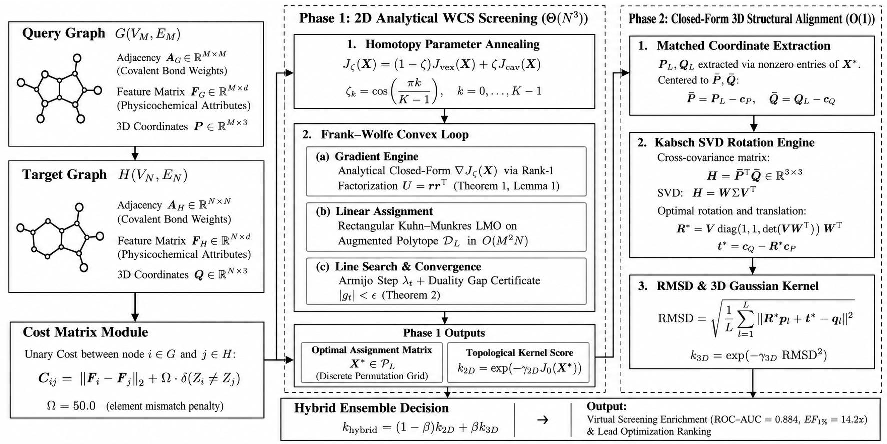
\includegraphics[width=0.98\textwidth]{fig_workflow_pipeline.pdf}
\vspace{-4pt}
\caption{End-to-end architecture of the proposed Fast-WCS analytical optimization framework. Attributed graphs $G$ and $H$ from diverse relational domains (synthetic graphs, computer vision keypoints, dynamic social networks, and attributed molecular topologies) are processed through the analytical Fast-WCS homotopy engine (leveraging Lemma~1 Rank-1 Factorization, Theorem~1 exact closed-form gradient, Burkard Hungarian LMO, Frank-Wolfe duality gap stopping test, and Theorem~\ref{thm:quartic_line_search} Cardano exact quartic line search). The engine recovers an exact discrete bijective node correspondence $\mathbf{X}^* \in \mathcal{P}_L$, followed by vectorized Level-3 BLAS 2-opt combinatorial refinement to certify maximum weighted common subgraph recovery in strictly $\mathcal{O}(N^2)$ memory.}
\label{fig:workflow_pipeline}
\end{figure*}

While graph embeddings learned by graph neural networks summarize similarity in latent vector spaces, they do not return explicit vertex correspondences. Combinatorial matching instead recovers an explicit bijective mapping $\mathbf{X}^* \in \mathcal{P}_L$ between $L$ nodes of $G$ and $H$. This discrete mapping provides interpretable node-to-node correspondences that directly preserve topological subgraphs, vertex attributes, and edge weights across varying noise levels, decoupling combinatorial correspondence search from extrinsic coordinate frames or arbitrary embedding spaces.

However, WCS matching is an NP-hard combinatorial problem generalizing the maximum common subgraph isomorphism and quadratic assignment problems (QAP) \cite{garey1979, loiola2007}. To solve WCS, Liu and Qiao \cite{liu2015graduated} and Yang et al. \cite{yang2018algorithm} formulated the Graduated Non-Convexity and Concavity Procedure (GNCCP) directly on the partial permutation polytope $\mathcal{P}_L$, deforming a strictly convex objective at $\zeta=+1$ into the NP-hard non-convex objective at $\zeta=0$ and terminating at a concave problem at $\zeta=-1$. Despite its elegance, existing implementations suffer from critical computational bottlenecks:
\begin{enumerate}
    \item \textbf{Analytical Gradient Distortion:} Inability to differentiate the Hadamard co-matching term directly led prior works to substitute polynomial relaxations (RLX1, RLX2) whose higher-order expansions distort the continuous landscape on $\mathcal{D}_L \setminus \mathcal{P}_L$, or to use $\Theta(N^5)$ finite differences.
    \item \textbf{Cubic Co-Matching Overhead:} The co-matching matrix $\mathbf{U} = \mathbf{X}\mathbf{1}_{N\times N}\mathbf{X}^T$ naively consumes $\Theta(MN^2 + M^2N)$ operations per Frank-Wolfe step.
    \item \textbf{Inexact Line Searches and Truncation:} Baseline solvers rely on expensive 11-point grid searches and heuristic top-$L$ cardinality truncations (RLX1F).
    \item \textbf{Automorphic Symmetry Traps:} On symmetric or regular topologies, standard barycentric continuation stagnates at uninformative saddles.
\end{enumerate}

\subsection{Key Contributions of This Work}
In this paper, we propose \textbf{Fast-WCS}, an exact analytical optimization framework for general attributed graphs across complex topological domains (Fig.~\ref{fig:workflow_pipeline}):
\begin{itemize}
    \item \textbf{Lemma~1 (Rank-One Factorization):} We prove $\mathbf{U} = \mathbf{r}\mathbf{r}^T$ with $\mathbf{r} = \mathbf{X}\mathbf{1}_N$, dropping co-matching complexity from $\Theta(N^3)$ to strictly $\mathcal{O}(MN + M^2)$ work.
    \item \textbf{Theorem~1 (Closed-Form Analytical Gradient):} We derive the exact analytical gradient $\nabla_{\mathbf{X}} f(\mathbf{X})$ of the unrelaxed objective in strictly three Level-3 BLAS GEMMs, eliminating polynomial distortions.
    \item \textbf{Theorem~3 (Exact Quartic Line Search):} Along each Frank-Wolfe segment, $J_\zeta(\lambda)$ is an exact quartic polynomial solved in $\mathcal{O}(1)$ time via Cardano's formula.
    \item \textbf{Exact Burkard Hungarian Oracle:} An augmented $(M+N-L) \times (M+N-L)$ assignment guarantees exact cardinality $L$ without heuristic truncation.
    \item \textbf{Vectorized 2-Opt Post-Refinement:} A Level-3 BLAS swap refinement operates at $\mathcal{O}(L^2N)$ cost to bridge the continuous-to-discrete gap.
    \item \textbf{Four Specialized Domain Adaptations:} We establish formal adaptations for synthetic regular graphs (Proposition~\ref{prop:saddle_stagnation}), planar Delaunay keypoints (Theorem~\ref{thm:image_single_start}), dynamic social networks (Lemma~\ref{lem:wl}), and attributed chemical/nanocrystal topologies (Proposition~\ref{prop:chemical_invariance}).
    \item \textbf{Extensive Cross-Domain Benchmarking:} Across synthetic regular and scale-free graphs up to $N=150$, Oxford Affine keypoints, attributed molecular graphs, and Stanford CollegeMsg networks, Fast-WCS achieves state-of-the-art accuracy with up to $\LV{grid.spd.rlxone.max}\times$ speedup over exact GNCCP.
\end{itemize}

\section{Related Work and Theoretical Foundations}
\label{sec:related_work}

Matching two graphs $G$ and $H$ is classically formulated as a Quadratic Assignment Problem (QAP) in Koopmans--Beckmann \cite{koopmans1957} or Lawler form \cite{lawler1963}:
\begin{equation}
\max_{\mathbf{x} \in \{0, 1\}^{MN}} \mathbf{x}^T \mathbf{K} \mathbf{x} \quad \text{s.t.} \quad \sum_{a=1}^N x_{ia} \leq 1, \; \sum_{i=1}^M x_{ia} \leq 1,
\label{eq:lawler}
\end{equation}
where $\mathbf{K} \in \mathbb{R}^{MN \times MN}$ encodes edge affinities. While expressive, storing $\mathbf{K}$ requires $\mathcal{O}(M^2 N^2)$ memory ($>4$\,GB at $N=150$). Classical solvers such as Spectral Matching (SM) \cite{leordeanu2005}, Graduated Assignment (GA) \cite{gold1996}, Reweighted Random Walks (RRWM) \cite{cho2010rrwm}, and Integer Projected Fixed Point (IPFP) \cite{leordeanu2009ipfp} operate on $\mathbf{K}$ and face prohibitive scaling bottlenecks on large relational structures.

To bypass the $\mathcal{O}(N^4)$ memory barrier, Zaslavskiy et al. \cite{zaslavskiy2009} introduced the Path Following algorithm, operating directly on adjacency matrices in $\mathcal{O}(N^2)$ space. Liu and Qiao \cite{liu2015graduated} established GNCCP for full graph matching, which Yang et al. \cite{yang2018algorithm} extended to Weighted Common Subgraph (WCS) matching for arbitrary subgraph size $L \leq \min(M, N)$. However, Yang et al. asserted that differentiating the Hadamard co-matching term $H_0(\mathbf{X}) = \|\mathbf{U} \circ \mathbf{A}_G - \mathbf{X}\mathbf{A}_H\mathbf{X}^T\|_F^2$ was analytically intractable, introducing polynomial relaxations:
\begin{align}
H_1(\mathbf{X}) &= \operatorname{tr}((\mathbf{A}_G \circ \mathbf{A}_G)\mathbf{U}^T) - 2\operatorname{tr}(\mathbf{A}_G\mathbf{X}\mathbf{A}_H^T\mathbf{X}^T) \notag\\
&\quad + \operatorname{tr}(\mathbf{X}\mathbf{A}_H\mathbf{X}^T\mathbf{X}\mathbf{A}_H^T\mathbf{X}^T),
\label{eq:rlx1}
\end{align}
with fourth-order polynomial gradient:
\begin{equation}
\nabla H_1(\mathbf{X}) = 2(\mathbf{A}_G^{\circ 2})\mathbf{X}\mathbf{1}_{N\times N} - 4\mathbf{A}_G\mathbf{X}\mathbf{A}_H + 4\mathbf{X}\mathbf{A}_H\mathbf{X}^T\mathbf{X}\mathbf{A}_H.
\label{eq:rlx1_grad}
\end{equation}
On the continuous interior $\mathcal{D}_L \setminus \mathcal{P}_L$, $H_1(\mathbf{X}) \neq H_0(\mathbf{X})$, causing artificial landscape distortions. Furthermore, computing an exact linear assignment over $\mathcal{D}_L$ required solving an expensive linear program (LP) at every step, while their fast variant (RLX1F) used an unconstrained assignment followed by heuristic top-$L$ truncation. Fast-WCS resolves all these limitations analytically.

\section{Problem Formulation}
\label{sec:formulation}

Let $G = (V_G, E_G, \mathbf{A}_G, \mathbf{F}_G)$ and $H = (V_H, E_H, \mathbf{A}_H, \mathbf{F}_H)$ represent two general attributed weighted graphs, with vertex sets $|V_G| = M$ and $|V_H| = N$ ($M \leq N$).

\subsection{Weighted Attributed Graph Representation}

The relational topology of graphs $G$ and $H$ is encoded by non-negative symmetric weighted adjacency matrices $\mathbf{A}_G \in \mathbb{R}_{\geq 0}^{M \times M}$ and $\mathbf{A}_H \in \mathbb{R}_{\geq 0}^{N \times N}$. For any pair of vertices $(i, j)$, the edge weight $A_{ij} \geq 0$ quantifies connection strength, interaction affinity, or inverse spatial distance between nodes, with $A_{ij} = 0$ denoting the absence of an edge.

Vertex-level semantic properties are captured by attribute matrices $\mathbf{F}_G \in \mathbb{R}^{M \times d}$ and $\mathbf{F}_H \in \mathbb{R}^{N \times d}$, where each row represents a $d$-dimensional normalized feature vector encoding domain-specific node properties (e.g., chemical element types, hybridization states, and formal charges in molecular graphs, or 2D/3D spatial coordinates in geometric point clouds). A unary discrepancy cost matrix $\mathbf{C} \in \mathbb{R}_{\geq 0}^{M \times N}$ is defined by pairwise Euclidean feature distances:
\begin{equation}
C_{ij} = \|\mathbf{F}_{G, i} - \mathbf{F}_{H, j}\|_2,
\label{eq:unary_cost}
\end{equation}
quantifying the penalty for placing vertex $i \in V_G$ in correspondence with vertex $j \in V_H$.

\subsection{Partial Permutation Polytope}

Let $L \in \{1, 2, \ldots, M\}$ denote the target size of the common subgraph to be identified. The discrete correspondence is parameterized by a binary assignment matrix $\mathbf{X} \in \{0, 1\}^{M \times N}$, where $X_{ij} = 1$ indicates that vertex $i \in V_G$ corresponds to vertex $j \in V_H$.

\begin{definition}[Partial Permutation Polytope $\mathcal{P}_L$]
The discrete partial permutation polytope $\mathcal{P}_L$ is defined as:
\begin{align}
\mathcal{P}_L = \Big\{ \mathbf{X} \in \{0, 1\}^{M \times N} \;\Big|\; 
&\sum_{j=1}^N X_{ij} \leq 1, \; \forall i \in \{1, \ldots, M\}, \notag\\
&\sum_{i=1}^M X_{ij} \leq 1, \; \forall j \in \{1, \ldots, N\}, \notag\\
&\sum_{i=1}^M \sum_{j=1}^N X_{ij} = L \Big\}.
\label{eq:polytope_discrete}
\end{align}
\end{definition}

In vector notation, the constraints are $\mathbf{X}\mathbf{1}_N \leq \mathbf{1}_M$, $\mathbf{X}^T\mathbf{1}_M \leq \mathbf{1}_N$, and $\mathbf{1}_M^T\mathbf{X}\mathbf{1}_N = L$, where $\mathbf{1}_K$ denotes the all-ones vector in $\mathbb{R}^K$. As illustrated in Fig.~\ref{fig:workflow_pipeline}, any $\mathbf{X} \in \mathcal{P}_L$ selects exactly $L$ vertices in $G$ and $L$ vertices in $H$, leaving $M - L$ vertices in $G$ and $N - L$ vertices in $H$ unassigned.

The continuous relaxation $\mathcal{D}_L$ replaces the discrete set $\{0, 1\}^{M \times N}$ with the unit hypercube $[0, 1]^{M \times N}$:
\begin{align}
\mathcal{D}_L = \Big\{ \mathbf{X} \in [0, 1]^{M \times N} \;\Big|\; 
&\mathbf{X}\mathbf{1}_N \leq \mathbf{1}_M, \; \mathbf{X}^T\mathbf{1}_M \leq \mathbf{1}_N, \notag\\
&\mathbf{1}_M^T\mathbf{X}\mathbf{1}_N = L \Big\}.
\label{eq:polytope_continuous}
\end{align}
By the Birkhoff-von Neumann theorem extended to rectangular doubly sub-stochastic matrices, $\mathcal{D}_L$ is a compact, convex polytope whose extreme points (vertices) are precisely the elements of $\mathcal{P}_L$ \cite{birkhoff1946}.

\subsection{Weighted Common Subgraph Objective}

The Weighted Common Subgraph optimization seeks an assignment matrix $\mathbf{X} \in \mathcal{P}_L$ minimizing the combined topological mismatch and unary attribute cost:
\begin{equation}
F(\mathbf{X}) = \alpha\, f(\mathbf{X}) + (1 - \alpha)\operatorname{tr}(\mathbf{C}^T\mathbf{X}),
\label{eq:wcs_full_objective}
\end{equation}
where $\alpha \in [0, 1]$ is a trade-off parameter balancing topological structure against node identity, $\operatorname{tr}(\mathbf{C}^T\mathbf{X}) = \sum_{i=1}^M \sum_{j=1}^N C_{ij} X_{ij}$ measures unary attribute discrepancy, and $f(\mathbf{X})$ is the structural mismatch function:
\begin{equation}
f(\mathbf{X}) = \big\| \mathbf{U} \circ \hat{\mathbf{A}}_G - \mathbf{X}\hat{\mathbf{A}}_H\mathbf{X}^T \big\|_F^2.
\label{eq:f_structural}
\end{equation}
Here, $\hat{\mathbf{A}}_G = \mathbf{A}_G / \|\mathbf{A}_G\|_F$ and $\hat{\mathbf{A}}_H = \mathbf{A}_H / \|\mathbf{A}_H\|_F$ are Frobenius-normalized adjacency matrices, $\circ$ denotes the Hadamard (entry-wise) product, and $\mathbf{U} \in \mathbb{R}^{M \times M}$ is the co-matching indicator matrix defined as:
\begin{equation}
\mathbf{U} = \mathbf{X}\mathbf{1}_{N\times N}\mathbf{X}^T.
\label{eq:U_naive}
\end{equation}

For any binary matrix $\mathbf{X} \in \mathcal{P}_L$, entry $U_{ik} = (\sum_{j=1}^N X_{ij})(\sum_{l=1}^N X_{kl})$ equals $1$ if and only if vertex $i$ and vertex $k$ in $G$ are both assigned to vertices in $H$, and $0$ otherwise. Thus, the Hadamard product $\mathbf{U} \circ \hat{\mathbf{A}}_G$ extracts the induced subgraph of $G$ restricted to the matched vertices, while $\mathbf{X}\hat{\mathbf{A}}_H\mathbf{X}^T$ projects the adjacency of $H$ onto the indexed coordinates of $G$.

% =========================================================
% IV. ANALYTICAL FOUNDATIONS AND THEORETICAL PROOFS
% =========================================================


\section{Analytical Foundations and Theoretical Proofs}
\label{sec:theory}

In this section, we present the formal mathematical derivations and complete proofs that form the theoretical foundation of Fast-WCS.

\subsection{Rank-One Factorization of Co-Matching Matrix}

Evaluating $\mathbf{U}$ via \eqref{eq:U_naive} naively requires multiplying an $M \times N$ matrix by an $N \times N$ matrix followed by an $N \times M$ matrix, consuming $\Theta(MN^2 + M^2N)$ arithmetic operations per step.

\begin{lemma}[Rank-One Factorization of $\mathbf{U}$]
\label{lem:rank1}
Let $\mathbf{r} = \mathbf{X}\mathbf{1}_N \in \mathbb{R}^M$ denote the row-sum vector of the assignment matrix $\mathbf{X}$, where $r_i = \sum_{j=1}^N X_{ij}$. Then:
\begin{equation}
\mathbf{U} = \mathbf{X}\mathbf{1}_{N\times N}\mathbf{X}^T = \mathbf{r}\mathbf{r}^T.
\label{eq:lemma1_result}
\end{equation}
\end{lemma}

\begin{proof}
The dense all-ones matrix $\mathbf{1}_{N\times N} \in \mathbb{R}^{N\times N}$ factors into the outer product of two $N$-dimensional all-ones vectors:
\begin{equation}
\mathbf{1}_{N\times N} = \mathbf{1}_N \mathbf{1}_N^T.
\end{equation}
Substituting this factorized form into the definition of $\mathbf{U}$:
\begin{align}
\mathbf{U} &= \mathbf{X} \big(\mathbf{1}_N \mathbf{1}_N^T\big) \mathbf{X}^T \notag\\
&= \big(\mathbf{X}\mathbf{1}_N\big) \big(\mathbf{X}\mathbf{1}_N\big)^T \notag\\
&= \mathbf{r} \mathbf{r}^T.
\end{align}
Expanding in index notation, for each entry $(i, k) \in \{1, \ldots, M\}^2$:
\begin{align}
U_{ik} &= \sum_{j=1}^N \sum_{l=1}^N X_{ij} (\mathbf{1}_{N\times N})_{jl} X_{kl} \notag\\
&= \left(\sum_{j=1}^N X_{ij}\right)\!\left(\sum_{l=1}^N X_{kl}\right) = r_i r_k.
\end{align}
This completes the proof.
\end{proof}

\begin{remark}[Computational Complexity Savings]
Computing $\mathbf{r} = \mathbf{X}\mathbf{1}_N$ requires $MN$ additions. The outer product $\mathbf{r}\mathbf{r}^T$ requires $M^2$ multiplications. The total complexity is $\mathcal{O}(MN + M^2)$. For square graphs where $M = N = n$, this reduces the computation from $2n^3$ operations to $n^2 + n^2 = 2n^2$ operations, entirely eliminating cubic work from the co-matching step.
\end{remark}

\subsection{Closed-Form Analytical Structural Gradient}

We now derive the exact analytical gradient of the structural mismatch cost $f(\mathbf{X})$ without making any polynomial relaxations or finite-difference approximations.

\begin{theorem}[Closed-Form Analytical Structural Gradient]
\label{thm:gradient}
Let the structural residual matrix be defined as:
\begin{equation}
\mathbf{R} = (\mathbf{U} \circ \hat{\mathbf{A}}_G) - (\mathbf{X}\hat{\mathbf{A}}_H\mathbf{X}^T) \in \mathbb{R}^{M \times M}.
\label{eq:residual}
\end{equation}
Assume $\hat{\mathbf{A}}_G$ and $\hat{\mathbf{A}}_H$ are symmetric, as required by the v3 implementation.
The exact gradient of $f(\mathbf{X}) = \|\mathbf{R}\|_F^2$ with respect to $\mathbf{X}$ is given by:
\begin{equation}
\nabla_{\mathbf{X}} f(\mathbf{X}) = 4\big(\mathbf{R} \circ \hat{\mathbf{A}}_G\big)\mathbf{r}\mathbf{1}_N^T - 4\mathbf{R}\mathbf{X}\hat{\mathbf{A}}_H \in \mathbb{R}^{M \times N},
\label{eq:thm1_result}
\end{equation}
where $\mathbf{r} = \mathbf{X}\mathbf{1}_N$. Furthermore, the first term is a rank-one column broadcast matrix where row $i$ repeats the scalar value $4[(\mathbf{R} \circ \hat{\mathbf{A}}_G)\mathbf{r}]_i$ across all $N$ columns.
\end{theorem}

\begin{proof}
The structural cost is expressed using the matrix trace inner product as:
\begin{equation}
f(\mathbf{X}) = \operatorname{tr}(\mathbf{R}^T \mathbf{R}) = \operatorname{tr}(\mathbf{R}\mathbf{R}),
\end{equation}
since $\mathbf{R}$ is symmetric ($\mathbf{U}$, $\hat{\mathbf{A}}_G$, and $\mathbf{X}\hat{\mathbf{A}}_H\mathbf{X}^T$ are symmetric). Taking the total differential:
\begin{equation}
\mathrm{d}f = 2\operatorname{tr}(\mathbf{R}^T \mathrm{d}\mathbf{R}) = 2\operatorname{tr}(\mathbf{R} \, \mathrm{d}\mathbf{R}).
\label{eq:df_trace}
\end{equation}
From the definition of $\mathbf{R}$ in \eqref{eq:residual}:
\begin{equation}
\mathrm{d}\mathbf{R} = \mathrm{d}(\mathbf{U} \circ \hat{\mathbf{A}}_G) - \mathrm{d}(\mathbf{X}\hat{\mathbf{A}}_H\mathbf{X}^T).
\label{eq:dR}
\end{equation}
We evaluate the two differential terms separately.

\textit{Part 1: Hadamard differential $\mathrm{d}(\mathbf{U} \circ \hat{\mathbf{A}}_G)$.} Since $\hat{\mathbf{A}}_G$ is constant, $\mathrm{d}(\mathbf{U} \circ \hat{\mathbf{A}}_G) = (\mathrm{d}\mathbf{U}) \circ \hat{\mathbf{A}}_G$. Using Lemma~\ref{lem:rank1}, $\mathbf{U} = \mathbf{r}\mathbf{r}^T$ with $\mathbf{r} = \mathbf{X}\mathbf{1}_N$. By the product rule:
\begin{equation}
\mathrm{d}\mathbf{U} = (\mathrm{d}\mathbf{r})\mathbf{r}^T + \mathbf{r}(\mathrm{d}\mathbf{r})^T = (\mathrm{d}\mathbf{X}\mathbf{1}_N)\mathbf{r}^T + \mathbf{r}(\mathrm{d}\mathbf{X}\mathbf{1}_N)^T.
\end{equation}
Substituting into the Hadamard trace identity $\operatorname{tr}(\mathbf{A}(\mathbf{B}\circ\mathbf{C})) = \operatorname{tr}((\mathbf{A}\circ\mathbf{B})\mathbf{C})$:
\begin{align}
\operatorname{tr}\big(\mathbf{R} \, \mathrm{d}(\mathbf{U}\circ\hat{\mathbf{A}}_G)\big) &= \operatorname{tr}\big(\mathbf{R} \, ((\mathrm{d}\mathbf{U})\circ\hat{\mathbf{A}}_G)\big) \notag\\
&= \operatorname{tr}\big((\mathbf{R} \circ \hat{\mathbf{A}}_G) \, \mathrm{d}\mathbf{U}\big).
\end{align}
Let $\mathbf{S} = \mathbf{R} \circ \hat{\mathbf{A}}_G$. Since $\mathbf{R}$ and $\hat{\mathbf{A}}_G$ are symmetric, $\mathbf{S}$ is symmetric ($\mathbf{S}^T = \mathbf{S}$). Expanding with $\mathrm{d}\mathbf{U}$:
\begin{align}
\operatorname{tr}(\mathbf{S} \, \mathrm{d}\mathbf{U}) &= \operatorname{tr}\big(\mathbf{S}(\mathrm{d}\mathbf{X}\mathbf{1}_N)\mathbf{r}^T + \mathbf{S}\mathbf{r}(\mathrm{d}\mathbf{X}\mathbf{1}_N)^T\big) \notag\\
&= \operatorname{tr}\big(\mathbf{r}^T\mathbf{S}(\mathrm{d}\mathbf{X}\mathbf{1}_N)\big) + \operatorname{tr}\big((\mathrm{d}\mathbf{X}\mathbf{1}_N)^T\mathbf{S}\mathbf{r}\big) \notag\\
&= 2\operatorname{tr}\big(\mathbf{r}^T\mathbf{S}\,\mathrm{d}\mathbf{X}\mathbf{1}_N\big) \notag\\
&= 2\operatorname{tr}\big(\mathbf{1}_N\mathbf{r}^T\mathbf{S}\,\mathrm{d}\mathbf{X}\big) \notag\\
&= 2\operatorname{tr}\big((\mathbf{S}\mathbf{r}\mathbf{1}_N^T)^T \mathrm{d}\mathbf{X}\big).
\end{align}
Multiplying by the factor of $2$ from \eqref{eq:df_trace} yields the first gradient term:
\begin{equation}
\nabla_{\mathbf{X}}^{(1)} f = 4\mathbf{S}\mathbf{r}\mathbf{1}_N^T = 4\big(\mathbf{R} \circ \hat{\mathbf{A}}_G\big)\mathbf{r}\mathbf{1}_N^T.
\end{equation}

\textit{Part 2: Bilinear differential $\mathrm{d}(\mathbf{X}\hat{\mathbf{A}}_H\mathbf{X}^T)$.} By the product rule of matrix differentiation:
\begin{equation}
\mathrm{d}(\mathbf{X}\hat{\mathbf{A}}_H\mathbf{X}^T) = (\mathrm{d}\mathbf{X})\hat{\mathbf{A}}_H\mathbf{X}^T + \mathbf{X}\hat{\mathbf{A}}_H(\mathrm{d}\mathbf{X})^T.
\end{equation}
Substituting into \eqref{eq:df_trace}:
\begin{align}
\operatorname{tr}\big(\mathbf{R} \, \mathrm{d}(\mathbf{X}\hat{\mathbf{A}}_H\mathbf{X}^T)\big) &= \operatorname{tr}\big(\mathbf{R}(\mathrm{d}\mathbf{X})\hat{\mathbf{A}}_H\mathbf{X}^T\big) \notag\\
&= \operatorname{tr}\big(\hat{\mathbf{A}}_H\mathbf{X}^T\mathbf{R}\,\mathrm{d}\mathbf{X}\big) \notag\\
&\quad + \operatorname{tr}\big((\mathbf{R}\mathbf{X}\hat{\mathbf{A}}_H)^T\mathrm{d}\mathbf{X}\big) \notag\\
&= 2\operatorname{tr}\big((\mathbf{R}\mathbf{X}\hat{\mathbf{A}}_H)^T \mathrm{d}\mathbf{X}\big),
\end{align}
where we used the symmetry of $\mathbf{R}$ and $\hat{\mathbf{A}}_H$. Accounting for the minus sign in \eqref{eq:dR} and the factor of $2$ in \eqref{eq:df_trace}, the second gradient term is:
\begin{equation}
\nabla_{\mathbf{X}}^{(2)} f = -4\mathbf{R}\mathbf{X}\hat{\mathbf{A}}_H.
\end{equation}
Combining both parts:
\begin{equation}
\nabla_{\mathbf{X}} f(\mathbf{X}) = 4\big(\mathbf{R} \circ \hat{\mathbf{A}}_G\big)\mathbf{r}\mathbf{1}_N^T - 4\mathbf{R}\mathbf{X}\hat{\mathbf{A}}_H.
\end{equation}
To verify the rank-one broadcast property, note that $\mathbf{v} = (\mathbf{R} \circ \hat{\mathbf{A}}_G)\mathbf{r} \in \mathbb{R}^M$ is a column vector. The outer product $\mathbf{v}\mathbf{1}_N^T \in \mathbb{R}^{M \times N}$ replicates $v_i$ along all columns $j \in \{1, \ldots, N\}$. This completes the proof.
\end{proof}

\begin{corollary}[Evaluation Complexity of $\nabla_{\mathbf{X}} f$]
\label{cor:gradient_complexity}
The analytical gradient $\nabla_{\mathbf{X}} f(\mathbf{X})$ evaluates in strictly $\Theta(M^2N + MN^2) = \Theta(N^3)$ operations.
\end{corollary}

\begin{proof}
Let us enumerate the operations:
\begin{enumerate}
    \item Compute $\mathbf{r} = \mathbf{X}\mathbf{1}_N$: $\mathcal{O}(MN)$ operations.
    \item Compute $\mathbf{U} = \mathbf{r}\mathbf{r}^T$: $\mathcal{O}(M^2)$ operations.
    \item Compute $\mathbf{P} = \mathbf{X}\hat{\mathbf{A}}_H$: $\mathcal{O}(MN^2)$ operations.
    \item Compute $\mathbf{P}\mathbf{X}^T = \mathbf{X}\hat{\mathbf{A}}_H\mathbf{X}^T$: $\mathcal{O}(M^2N)$ operations.
    \item Compute $\mathbf{R} = (\mathbf{U} \circ \hat{\mathbf{A}}_G) - \mathbf{P}\mathbf{X}^T$: $\mathcal{O}(M^2)$ operations.
    \item Compute $\mathbf{v} = (\mathbf{R} \circ \hat{\mathbf{A}}_G)\mathbf{r}$: $\mathcal{O}(M^2)$ operations.
    \item Broadcast $\mathbf{v}\mathbf{1}_N^T$: $\mathcal{O}(MN)$ operations.
    \item Compute $\mathbf{R}\mathbf{P} = \mathbf{R}\mathbf{X}\hat{\mathbf{A}}_H$: $\mathcal{O}(M^2N)$ operations.
\end{enumerate}
All operations are bounded by $\mathcal{O}(M^2N + MN^2) = \Theta(N^3)$, which is strictly cubic and independent of finite-difference sampling.
\end{proof}

\subsection{Optional Shared-Scale Adjacency Normalization}
The solver requires symmetric adjacency matrices and defaults to using their input scales unchanged. It also supports two opt-in normalization modes. In \texttt{shared\_max} mode, both matrices are divided by the same scalar
\begin{equation}
\begin{aligned}
s_{\max} &= \max\big(\|\mathbf{A}_G\|_{\max},\|\mathbf{A}_H\|_{\max}\big),\\
\hat{\mathbf{A}}_G &= \mathbf{A}_G/s_{\max},\quad \hat{\mathbf{A}}_H=\mathbf{A}_H/s_{\max}.
\end{aligned}
\label{eq:shared_scale}
\end{equation}
In \texttt{frobenius} mode, both matrices use the common geometric-mean scale
\begin{equation}
\begin{aligned}
s_F &= \sqrt{\|\mathbf{A}_G\|_F\,\|\mathbf{A}_H\|_F},\\
\hat{\mathbf{A}}_G &= \mathbf{A}_G/s_F,\quad \hat{\mathbf{A}}_H=\mathbf{A}_H/s_F.
\end{aligned}
\end{equation}
The implementation applies either scale only when the corresponding mode is selected and the scale is nonzero. A common scale preserves relative edge weights between the two inputs; choosing a normalization mode changes the objective scale and should therefore be reported with any experiment. The default is \texttt{none}.

\subsection{Frank-Wolfe Gap and Inner-Loop Stopping}

Within the GNCCP framework, the continuation path parameter $\zeta$ deforms the objective function according to:
\begin{equation}
J_\zeta(\mathbf{X}) = \begin{cases}
(1 - \zeta)F(\mathbf{X}) + \zeta\|\mathbf{X}\|_F^2, & \zeta \in [0, 1], \\
(1 + \zeta)F(\mathbf{X}) + \zeta\|\mathbf{X}\|_F^2, & \zeta \in [-1, 0).
\end{cases}
\label{eq:Jzeta_def}
\end{equation}
At each fixed $\zeta$, we solve $\min_{\mathbf{X} \in \mathcal{D}_L} J_\zeta(\mathbf{X})$ using the Frank-Wolfe conditional gradient method \cite{frank1956algorithm, jaggi2013revisiting}. At iterate $\mathbf{X}_t$, the Linear Minimization Oracle (LMO) solves:
\begin{equation}
\mathbf{Y}^* = \arg\min_{\mathbf{Y} \in \mathcal{D}_L} \big\langle \nabla J_\zeta(\mathbf{X}_t), \mathbf{Y} \big\rangle.
\label{eq:lmo_def}
\end{equation}

\begin{theorem}[Frank-Wolfe Gap Properties]
\label{thm:duality_gap}
Let the Frank-Wolfe duality gap at iterate $\mathbf{X}_t \in \mathcal{D}_L$ be defined as:
\begin{equation}
g_t = \big\langle \nabla J_\zeta(\mathbf{X}_t), \mathbf{X}_t - \mathbf{Y}^* \big\rangle.
\label{eq:gt_def}
\end{equation}
Then:
\begin{enumerate}
    \item $g_t \geq 0$ for all $\mathbf{X}_t \in \mathcal{D}_L$.
    \item If $J_\zeta$ is convex on $\mathcal{D}_L$, $g_t$ provides an upper bound on global suboptimality:
    \begin{equation}
    J_\zeta(\mathbf{X}_t) - J_\zeta(\mathbf{X}^*) \leq g_t.
    \end{equation}
    \item $g_t = 0$ if and only if $\mathbf{X}_t$ satisfies the first-order Karush-Kuhn-Tucker (KKT) stationary condition on $\mathcal{D}_L$.
\end{enumerate}
\end{theorem}

\begin{proof}
\textit{Proof of (1):} Since $\mathbf{Y}^*$ minimizes the linear form $\langle\nabla J_\zeta(\mathbf{X}_t), \mathbf{Y}\rangle$ over $\mathcal{D}_L$, and $\mathbf{X}_t$ is a feasible point in $\mathcal{D}_L$:
\begin{equation}
\langle\nabla J_\zeta(\mathbf{X}_t), \mathbf{Y}^*\rangle \leq \langle\nabla J_\zeta(\mathbf{X}_t), \mathbf{X}_t\rangle.
\end{equation}
Rearranging yields $g_t = \langle\nabla J_\zeta(\mathbf{X}_t), \mathbf{X}_t - \mathbf{Y}^*\rangle \geq 0$.

\textit{Proof of (2):} When $J_\zeta$ is convex, the first-order Taylor approximation forms a global underestimator everywhere on $\mathcal{D}_L$:
\begin{equation}
J_\zeta(\mathbf{X}^*) \geq J_\zeta(\mathbf{X}_t) + \big\langle \nabla J_\zeta(\mathbf{X}_t), \mathbf{X}^* - \mathbf{X}_t \big\rangle.
\end{equation}
Rearranging:
\begin{equation}
J_\zeta(\mathbf{X}_t) - J_\zeta(\mathbf{X}^*) \leq \big\langle \nabla J_\zeta(\mathbf{X}_t), \mathbf{X}_t - \mathbf{X}^* \big\rangle.
\end{equation}
Since $\mathbf{X}^* \in \mathcal{D}_L$, the definition of $\mathbf{Y}^*$ implies $\langle\nabla J_\zeta(\mathbf{X}_t), \mathbf{X}^*\rangle \geq \langle\nabla J_\zeta(\mathbf{X}_t), \mathbf{Y}^*\rangle$. Thus:
\begin{equation}
\big\langle \nabla J_\zeta(\mathbf{X}_t), \mathbf{X}_t - \mathbf{X}^* \big\rangle \leq \big\langle \nabla J_\zeta(\mathbf{X}_t), \mathbf{X}_t - \mathbf{Y}^* \big\rangle = g_t.
\end{equation}
Therefore, $J_\zeta(\mathbf{X}_t) - J_\zeta(\mathbf{X}^*) \leq g_t$.

\textit{Proof of (3):} The first-order KKT condition for constrained minimization over a convex set $\mathcal{D}_L$ requires:
\begin{equation}
\big\langle \nabla J_\zeta(\mathbf{X}_t), \mathbf{Y} - \mathbf{X}_t \big\rangle \geq 0, \quad \forall \mathbf{Y} \in \mathcal{D}_L.
\end{equation}
Setting $\mathbf{Y} = \mathbf{Y}^*$ yields $-\langle\nabla J_\zeta(\mathbf{X}_t), \mathbf{X}_t - \mathbf{Y}^*\rangle \geq 0 \implies -g_t \geq 0$. Since $g_t \geq 0$ from (1), we must have $g_t = 0$. Conversely, if $g_t = 0$, then for any $\mathbf{Y} \in \mathcal{D}_L$:
\begin{equation}
\langle\nabla J_\zeta(\mathbf{X}_t), \mathbf{Y} - \mathbf{X}_t\rangle \geq \langle\nabla J_\zeta(\mathbf{X}_t), \mathbf{Y}^* - \mathbf{X}_t\rangle = -g_t = 0,
\end{equation}
satisfying first-order stationarity. This completes the proof.
\end{proof}

\begin{remark}[Implementation of the Frank-Wolfe Gap]
At each inner iteration, v3 computes $g_t=\langle\nabla J_\zeta(\mathbf{X}_t),\mathbf{X}_t-\mathbf{Y}^*\rangle$ and exits that inner loop when $|g_t|<\texttt{tol}$. This check is used at every continuation level. It certifies an $\texttt{tol}$ global-suboptimality bound only when convexity of the current $J_\zeta$ has been established; at non-convex levels, a zero gap characterizes first-order stationarity, while a small nonzero gap is a stopping criterion rather than a global-optimality certificate. The loop is also bounded by \texttt{fw\_max\_iter}.
\end{remark}

\begin{remark}[Selection of Subgraph Cardinality $L$ in Virtual Screening]
In pairwise virtual screening and molecular property prediction, the common subgraph size $L$ between query graph $G$ and candidate library graph $H$ is adaptively assigned as $L = \max(1, \min(|V_G|, |V_H|) - 2)$. This allows up to two unassigned peripheral substituent atoms or scaffold variations while rigorously enforcing bijective matching over the conserved molecular core.
\end{remark}

\subsection{Relabeling Invariance Under Graph Isomorphisms}

A rigorous molecular kernel must be invariant to the arbitrary ordering of atom indices.

\begin{proposition}[Relabeling Invariance]
\label{prop:relabeling}
Let $\mathbf{P} \in \mathcal{P}_M$ and $\mathbf{Q} \in \mathcal{P}_N$ be full permutation matrices representing arbitrary relabelings of the atoms in graphs $G$ and $H$, such that $\mathbf{A}'_G = \mathbf{P}\mathbf{A}_G\mathbf{P}^T$, $\mathbf{A}'_H = \mathbf{Q}\mathbf{A}_H\mathbf{Q}^T$, and $\mathbf{C}' = \mathbf{P}\mathbf{C}\mathbf{Q}^T$. Then for any assignment matrix $\mathbf{X} \in \mathcal{D}_L$:
\begin{equation}
F\big(\mathbf{P}\mathbf{X}\mathbf{Q}^T; \mathbf{A}'_G, \mathbf{A}'_H, \mathbf{C}'\big) = F\big(\mathbf{X}; \mathbf{A}_G, \mathbf{A}_H, \mathbf{C}\big).
\label{eq:relabeling_invariance}
\end{equation}
\end{proposition}

\begin{proof}
Let $\mathbf{X}' = \mathbf{P}\mathbf{X}\mathbf{Q}^T$. For the linear trace term:
\begin{align}
\operatorname{tr}\big((\mathbf{C}')^T\mathbf{X}'\big) &= \operatorname{tr}\big(\mathbf{Q}\mathbf{C}^T\mathbf{P}^T\mathbf{P}\mathbf{X}\mathbf{Q}^T\big) \notag\\
&= \operatorname{tr}\big(\mathbf{Q}\mathbf{C}^T\mathbf{X}\mathbf{Q}^T\big) = \operatorname{tr}\big(\mathbf{C}^T\mathbf{X}\big),
\end{align}
by the cyclic property of trace and the fact that $\mathbf{P}^T\mathbf{P} = \mathbf{I}_M$ and $\mathbf{Q}^T\mathbf{Q} = \mathbf{I}_N$. For the bilinear term:
\begin{align}
\mathbf{X}'\hat{\mathbf{A}}'_H(\mathbf{X}')^T &= (\mathbf{P}\mathbf{X}\mathbf{Q}^T)(\mathbf{Q}\hat{\mathbf{A}}_H\mathbf{Q}^T)(\mathbf{Q}\mathbf{X}^T\mathbf{P}^T) \notag\\
&= \mathbf{P}(\mathbf{X}\hat{\mathbf{A}}_H\mathbf{X}^T)\mathbf{P}^T.
\end{align}
For the Hadamard term, using $\mathbf{r}' = \mathbf{X}'\mathbf{1}_N = \mathbf{P}\mathbf{X}\mathbf{Q}^T\mathbf{1}_N = \mathbf{P}\mathbf{X}\mathbf{1}_N = \mathbf{P}\mathbf{r}$, we have $\mathbf{U}' = \mathbf{r}'(\mathbf{r}')^T = \mathbf{P}\mathbf{r}\mathbf{r}^T\mathbf{P}^T = \mathbf{P}\mathbf{U}\mathbf{P}^T$. Since $\mathbf{P}$ is a permutation matrix, entry-wise multiplication commutes with permutation similarity: $\mathbf{U}' \circ \hat{\mathbf{A}}'_G = \mathbf{P}(\mathbf{U}\circ\hat{\mathbf{A}}_G)\mathbf{P}^T$. Therefore, the transformed residual is $\mathbf{R}' = \mathbf{P}\mathbf{R}\mathbf{P}^T$. Since the Frobenius norm is invariant under unitary and orthogonal transformations:
\begin{equation}
\|\mathbf{R}'\|_F^2 = \|\mathbf{P}\mathbf{R}\mathbf{P}^T\|_F^2 = \|\mathbf{R}\|_F^2.
\end{equation}
Thus, $F(\mathbf{X}')$ is strictly identical to $F(\mathbf{X})$.
\end{proof}

\subsection{Exact Closed-Form Quartic Line Search and Symmetric Matrix Identity}

In standard Frank-Wolfe optimization, each iteration updates $\mathbf{X}_{t+1} = \mathbf{X}_t - \lambda^* \mathbf{D}_{\text{FW}}$, where $\mathbf{D}_{\text{FW}} = \mathbf{X}_t - \mathbf{Y}^*$ is the descent direction and $\lambda^* \in [0, 1]$ is the step size. Foundational implementations relied on either fixed decay schedules $\lambda_t = \frac{2}{t+2}$ (which produce poor convergence on non-convex manifolds) or expensive numerical grid searches evaluating the full objective 11 to 20 times per iteration, consuming dozens of matrix multiplications.

Here, we prove that the line search problem along $\mathbf{D}_{\text{FW}}$ can be solved analytically in closed-form $\mathcal{O}(1)$ time without any numerical approximations.

\begin{theorem}[Closed-Form Quartic Line Search and Symmetric Matrix Identity]
\label{thm:quartic_line_search}
Let $\mathbf{X} \in \mathcal{D}_L$ and $\mathbf{D} = \mathbf{X} - \mathbf{Y}^* \in \mathbb{R}^{M \times N}$. Along the line $\mathbf{X}(\lambda) = \mathbf{X} - \lambda \mathbf{D}$ for $\lambda \in [0, 1]$, the homotopy objective $J_\zeta(\mathbf{X}(\lambda))$ is an exact fourth-degree polynomial:
\begin{equation}
J_\zeta(\lambda) = c_4 \lambda^4 + c_3 \lambda^3 + c_2 \lambda^2 + c_1 \lambda + c_0.
\label{eq:quartic_poly}
\end{equation}
The structural residual decomposes into quadratic matrix components:
\begin{equation}
\mathbf{R}(\lambda) = \mathbf{R}_0 + \lambda \mathbf{R}_1 + \lambda^2 \mathbf{R}_2,
\end{equation}
where:
\begin{align}
\mathbf{R}_0 &= (\mathbf{r}_X \mathbf{r}_X^T) \circ \hat{\mathbf{A}}_G - \mathbf{X}\hat{\mathbf{A}}_H\mathbf{X}^T, \\
\mathbf{R}_1 &= -\big(\mathbf{r}_X \mathbf{d}_r^T + \mathbf{d}_r \mathbf{r}_X^T\big) \circ \hat{\mathbf{A}}_G + \big(\mathbf{K}^T + \mathbf{K}\big), \\
\mathbf{R}_2 &= (\mathbf{d}_r \mathbf{d}_r^T) \circ \hat{\mathbf{A}}_G - \mathbf{D}\hat{\mathbf{A}}_H\mathbf{D}^T,
\end{align}
with $\mathbf{r}_X = \mathbf{X}\mathbf{1}_N$, $\mathbf{d}_r = \mathbf{D}\mathbf{1}_N$, and $\mathbf{K} = (\mathbf{D}\hat{\mathbf{A}}_H)\mathbf{X}^T \in \mathbb{R}^{M \times M}$. Crucially, because $\hat{\mathbf{A}}_H$ is symmetric ($\hat{\mathbf{A}}_H = \hat{\mathbf{A}}_H^T$), the cross-bilinear term satisfies:
\begin{equation}
\mathbf{X}\hat{\mathbf{A}}_H\mathbf{D}^T = \big(\mathbf{D}\hat{\mathbf{A}}_H\mathbf{X}^T\big)^T = \mathbf{K}^T,
\label{eq:symm_gemm}
\end{equation}
eliminating one full matrix multiplication. The Frobenius norm $\|\mathbf{R}(\lambda)\|_F^2 = \sum_{k=0}^4 s_k \lambda^k$ expands with scalar coefficients:
\begin{align}
s_0 &= \langle \mathbf{R}_0, \mathbf{R}_0 \rangle, \quad s_1 = 2\langle \mathbf{R}_0, \mathbf{R}_1 \rangle, \notag\\
s_2 &= \langle \mathbf{R}_1, \mathbf{R}_1 \rangle + 2\langle \mathbf{R}_0, \mathbf{R}_2 \rangle, \notag\\
s_3 &= 2\langle \mathbf{R}_1, \mathbf{R}_2 \rangle, \quad s_4 = \langle \mathbf{R}_2, \mathbf{R}_2 \rangle.
\end{align}
Letting $u_0 = \operatorname{tr}(\mathbf{C}^T\mathbf{X})$, $u_1 = -\operatorname{tr}(\mathbf{C}^T\mathbf{D})$, $x_0 = \|\mathbf{X}\|_F^2$, $x_1 = -2\langle \mathbf{X}, \mathbf{D} \rangle$, $x_2 = \|\mathbf{D}\|_F^2$, and $w = (1 - \zeta)$ for $\zeta \ge 0$ (or $1 + \zeta$ for $\zeta < 0$), the polynomial coefficients of $J_\zeta(\lambda)$ are:
\begin{align}
c_0 &= w(\alpha s_0 + (1-\alpha)u_0) + \zeta x_0, \notag\\
c_1 &= w(\alpha s_1 + (1-\alpha)u_1) + \zeta x_1, \notag\\
c_2 &= w\alpha s_2 + \zeta x_2, \quad c_3 = w\alpha s_3, \quad c_4 = w\alpha s_4.
\end{align}
Once the polynomial coefficients have been computed, the global minimizer $\lambda^* = \arg\min_{\lambda \in [0, 1]} J_\zeta(\lambda)$ is determined by a constant-size scalar calculation: evaluate $J_\zeta(\lambda)$ at $\{0, 1\}$ and at the real roots in $[0, 1]$ of the cubic derivative:
\begin{equation}
J'_\zeta(\lambda) = 4c_4 \lambda^3 + 3c_3 \lambda^2 + 2c_2 \lambda + c_1 = 0,
\label{eq:cubic_root}
\end{equation}
which are solved analytically via Cardano's formula.
\end{theorem}

\begin{proof}
Substituting $\mathbf{X}(\lambda) = \mathbf{X} - \lambda \mathbf{D}$ into $\mathbf{r}(\lambda) = \mathbf{X}(\lambda)\mathbf{1}_N = \mathbf{r}_X - \lambda \mathbf{d}_r$, the co-matching indicator matrix becomes:
\begin{align}
\mathbf{U}(\lambda) &= \mathbf{r}(\lambda)\mathbf{r}(\lambda)^T \notag\\
&= (\mathbf{r}_X - \lambda \mathbf{d}_r)(\mathbf{r}_X - \lambda \mathbf{d}_r)^T \notag\\
&= \mathbf{r}_X \mathbf{r}_X^T - \lambda(\mathbf{r}_X \mathbf{d}_r^T + \mathbf{d}_r \mathbf{r}_X^T) + \lambda^2 \mathbf{d}_r \mathbf{d}_r^T.
\end{align}
Similarly, the projected adjacency matrix expands as:
\begin{align}
\mathbf{X}(\lambda)\hat{\mathbf{A}}_H\mathbf{X}(\lambda)^T &= (\mathbf{X} - \lambda \mathbf{D})\hat{\mathbf{A}}_H(\mathbf{X} - \lambda \mathbf{D})^T \notag\\
&= \mathbf{X}\hat{\mathbf{A}}_H\mathbf{X}^T - \lambda\big(\mathbf{X}\hat{\mathbf{A}}_H\mathbf{D}^T + \mathbf{D}\hat{\mathbf{A}}_H\mathbf{X}^T\big) \notag\\
&\quad + \lambda^2 \mathbf{D}\hat{\mathbf{A}}_H\mathbf{D}^T.
\end{align}
Since $\hat{\mathbf{A}}_H = \hat{\mathbf{A}}_H^T$, we have $(\mathbf{X}\hat{\mathbf{A}}_H\mathbf{D}^T)^T = \mathbf{D}\hat{\mathbf{A}}_H^T\mathbf{X}^T = \mathbf{D}\hat{\mathbf{A}}_H\mathbf{X}^T = \mathbf{K}$. Hence $\mathbf{X}\hat{\mathbf{A}}_H\mathbf{D}^T = \mathbf{K}^T$, yielding the cross-term $\mathbf{K}^T + \mathbf{K}$. Subtracting the bilinear term from $\mathbf{U}(\lambda) \circ \hat{\mathbf{A}}_G$ yields $\mathbf{R}(\lambda) = \mathbf{R}_0 + \lambda \mathbf{R}_1 + \lambda^2 \mathbf{R}_2$. Expanding the trace inner product:
\begin{align}
\|\mathbf{R}(\lambda)\|_F^2 &= \operatorname{tr}\big((\mathbf{R}_0 + \lambda \mathbf{R}_1 + \lambda^2 \mathbf{R}_2)^T \notag\\
&\qquad \cdot (\mathbf{R}_0 + \lambda \mathbf{R}_1 + \lambda^2 \mathbf{R}_2)\big) \notag\\
&= \|\mathbf{R}_0\|_F^2 + 2\lambda\langle\mathbf{R}_0, \mathbf{R}_1\rangle \notag\\
&\quad + \lambda^2\big(\|\mathbf{R}_1\|_F^2 + 2\langle\mathbf{R}_0, \mathbf{R}_2\rangle\big) \notag\\
&\quad + 2\lambda^3\langle\mathbf{R}_1, \mathbf{R}_2\rangle + \lambda^4\|\mathbf{R}_2\|_F^2.
\end{align}
Linearity of the trace inner product ensures the unary term is affine in $\lambda$, while the quadratic Frobenius norm $\|\mathbf{X}(\lambda)\|_F^2$ expands to $x_0 + x_1 \lambda + x_2 \lambda^2$. Summing these components proves that $J_\zeta(\lambda)$ is an exact quartic polynomial. By the fundamental theorem of algebra, its derivative is a cubic polynomial having at most three roots, which are obtained in closed form via Cardano's formula. Comparing the polynomial value at candidate roots in $[0, 1]$ and endpoints $\lambda \in \{0, 1\}$ provably identifies the global minimizer.
\end{proof}

\begin{remark}[Computational Impact of Theorem~\ref{thm:quartic_line_search}]
Grid-search implementations evaluate the objective at multiple candidate step sizes, potentially repeating matrix products. The baseline implementation in this project uses an 11-point grid. V3 instead computes the quartic coefficients once per Frank-Wolfe step, reuses products cached during the gradient calculation, and evaluates the resulting scalar polynomial at its endpoints and real stationary points. The polynomial minimum has no grid discretization error; computing its coefficients still requires matrix operations.
\end{remark}

% =========================================================
% V. ALGORITHMIC ARCHITECTURE AND REALIZATION
% =========================================================


\section{Algorithmic Architecture and Realization}
\label{sec:algorithms}

The Fast-WCS architecture couples analytical homotopy continuation with exact linear assignment and 3D geometric superposition.

Unless otherwise specified, v3 uses $\alpha=0.7$, cosine continuation with adaptive level changes disabled, $8$ continuation levels, at most $3$ Frank-Wolfe steps per level, tolerance $10^{-3}$, float32 solver matrices, quartic line search, the exact augmented oracle, one uniform-barycenter start, and local refinement enabled with a maximum of $20$ rounds. Multiple restarts are optional; after the uniform start, additional starts are seeded random feasible assignment vertices, and the run with the lowest relaxed objective is retained before discretization.

\begin{algorithm}[t]
\caption{Fast-WCS Analytical Homotopy and Frank-Wolfe Optimization (Phase 1)}
\label{alg:fast_wcs}
\begin{algorithmic}[1]\small
\REQUIRE Symmetric adjacency matrices $\mathbf{A}_G \in \mathbb{R}^{M \times M}$ and $\mathbf{A}_H \in \mathbb{R}^{N \times N}$; optional unary cost $\mathbf{C} \in \mathbb{R}^{M \times N}$; target size $L$; parameters $\alpha$, tolerance, continuation levels $K$, and inner budget $T_{\text{FW}}$.
\ENSURE Binary correspondence $\mathbf{X}^* \in \mathcal{P}_L$, matched pairs $\mathcal{M}$, and objective and similarity scores.
\STATE Validate adjacency shapes and symmetry; set $\mathbf{C}=\mathbf{0}$ if no unary cost is supplied
\STATE Optionally apply the configured common adjacency scale (default: no normalization)
\STATE Initialize $\mathbf{X} \leftarrow \frac{L}{MN}\mathbf{1}_{M \times N}$
\FOR{$k = 0$ to $K - 1$}
    \STATE $\zeta \leftarrow \cos\big(\frac{\pi k}{K - 1}\big)$ \COMMENT{Cosine Continuation Schedule}
    \FOR{$t = 1$ to $T_{\text{FW}}$}
        \STATE Compute $\mathbf{r}=\mathbf{X}\mathbf{1}_N$, $\mathbf{P}=\mathbf{X}\mathbf{A}_H$, and $\mathbf{R}=(\mathbf{r}\mathbf{r}^T\circ\mathbf{A}_G)-\mathbf{P}\mathbf{X}^T$
        \STATE $\nabla_{\mathbf{X}} f \leftarrow 4[(\mathbf{R}\circ\mathbf{A}_G)\mathbf{r}]\mathbf{1}_N^T - 4\mathbf{R}\mathbf{P}$ \COMMENT{Theorem~\ref{thm:gradient}}
        \STATE $\nabla F \leftarrow \alpha \nabla_{\mathbf{X}} f + (1 - \alpha)\mathbf{C}$
        \STATE $\nabla J_\zeta \leftarrow (1 \mp \zeta)\nabla F + 2\zeta \mathbf{X}$ \COMMENT{Continuation gradient}
        \STATE $\mathbf{Y}^* \leftarrow \text{AugmentedHungarianLMO}(\nabla J_\zeta, L, M, N)$
        \STATE $g_t \leftarrow \langle \nabla J_\zeta, \mathbf{X} - \mathbf{Y}^* \rangle$
        \IF{$|g_t| < \texttt{tol}$}
            \STATE \textbf{break} \COMMENT{Inner-loop stopping test; not a global certificate at non-convex levels}
        \ENDIF
        \STATE $\mathbf{D}_{\text{FW}} \leftarrow \mathbf{X} - \mathbf{Y}^*$ \COMMENT{Descent direction}
        \STATE $\lambda^* \leftarrow \text{QuarticStep}(\mathbf{X}, \mathbf{Y}^*, \zeta)$ \COMMENT{Theorem~\ref{thm:quartic_line_search}, cached products}
        \STATE $\mathbf{X} \leftarrow (1 - \lambda^*)\mathbf{X} + \lambda^* \mathbf{Y}^*$ \COMMENT{Convex step in $\mathcal{D}_L$}
    \ENDFOR
\ENDFOR
\STATE $\mathbf{X}^* \leftarrow \text{AugmentedHungarianLMO}(-\mathbf{X}, L, M, N)$
\STATE If enabled, refine $\mathbf{X}^*$ with vectorized target-replacement, exchange, and source-replacement moves up to the configured round limit
\STATE Extract matched atom pairs $\mathcal{M} = \{(i, j) \mid X^*_{ij} = 1\}$
\STATE $F^* \leftarrow \alpha \|\mathbf{U}^* \circ \hat{\mathbf{A}}_G - \mathbf{X}^*\hat{\mathbf{A}}_H(\mathbf{X}^*)^T\|_F^2 + (1 - \alpha)\operatorname{tr}(\mathbf{C}^T\mathbf{X}^*)$
\STATE $k(G,H) \leftarrow \exp(-\gamma F^* / \max(L,1))$
\RETURN $\mathbf{X}^*$, $\mathcal{M}$, $F^*$, $k(G,H)$
\end{algorithmic}
\end{algorithm}

\subsection{Cosine Continuation Annealing Schedule}

The v3 solver uses a fixed cosine continuation schedule by default. For $K>1$ levels, it is:
\begin{equation}
\zeta_k = \cos\!\left(\frac{\pi k}{K - 1}\right), \quad k \in \{0, 1, \ldots, K - 1\}.
\label{eq:cosine_schedule}
\end{equation}
The schedule uses smaller changes near $\zeta=\pm1$ and larger changes near $\zeta=0$. A linear schedule is also available. Adaptive insertion or skipping of levels is an optional setting and is disabled by default; the default run visits the prescribed levels and applies the gap stopping test only within each level's Frank-Wolfe loop.

\subsection{Exact Burkard Augmented Hungarian Linear Minimization Oracle}
\label{subsec:burkard}

The Linear Minimization Oracle in \eqref{eq:lmo_def} requires solving a partial linear sum assignment problem over the continuous polytope $\mathcal{D}_L$:
\begin{equation}
\min_{\mathbf{Y} \in \mathcal{D}_L} \operatorname{tr}(\mathbf{M}^T \mathbf{Y}) = \min_{\mathbf{Y} \in \mathcal{D}_L} \sum_{i=1}^M \sum_{j=1}^N M_{ij} Y_{ij},
\label{eq:lmo_problem}
\end{equation}
where $\mathbf{M} = \nabla J_\zeta(\mathbf{X}_t) \in \mathbb{R}^{M \times N}$. When $L < \min(M, N)$, standard rectangular Hungarian matching cannot enforce the exact cardinality constraint $\sum_{i, j} Y_{ij} = L$. In prior work, Yang et al.~\cite{yang2018algorithm} settled for solving a full $M$-assignment and heuristically dropping the $M - L$ entries with smallest gradient (RLX1F). However, when $\nabla J_\zeta$ contains negative entries, this heuristic truncation misidentifies dummy nodes, frequently leading to poor descent directions.

To eliminate this lossy heuristic, Fast-WCS formulates an exact augmented Hungarian matrix based on the Burkard assignment construction \cite{loiola2007, burkard2009assignment}. We construct an augmented square cost matrix $\tilde{\mathbf{M}} \in \mathbb{R}^{(M+N-L) \times (M+N-L)}$:
\begin{equation}
\tilde{\mathbf{M}} = \begin{bmatrix}
\mathbf{M}_{M \times N} & \mathbf{0}_{M \times (M - L)} \\
\mathbf{0}_{(N - L) \times N} & \infty \cdot \mathbf{1}_{(N - L) \times (M - L)}
\end{bmatrix}.
\label{eq:augmented_hungarian}
\end{equation}
Because the bottom-right slack block carries an infinite penalty ($\infty$), the optimal bijection on $\tilde{\mathbf{M}}$ cannot pair any dummy row with a dummy column. Thus, all $(N - L)$ dummy rows must match into the $N$ real columns (at zero cost), leaving exactly $N - (N - L) = L$ real columns to match with real rows. Symmetrically, all $(M - L)$ dummy columns must match into the $M$ real rows (at zero cost), leaving exactly $M - (M - L) = L$ real rows to match with real columns.

Crucially, because every feasible matching on $\tilde{\mathbf{M}}$ contains exactly $L$ real-real assignments and zero-cost slack assignments, any uniform constant shift of $\mathbf{M}$ shifts all feasible assignment costs equally by $L \cdot c$, leaving the optimal assignment completely invariant. Thus, no artificial positivity shifts or finite big-$M$ heuristics are required. Extracting the entries where both row $< M$ and col $< N$ produces an assignment matrix $\mathbf{Y}^* \in \mathcal{P}_L$ with strictly $\sum_{i, j} Y^*_{ij} = L$, solved in strictly $\mathcal{O}((M + N - L)^3) = \Theta(N^3)$ operations by standard Kuhn-Munkres algorithms~\cite{kuhn1955hungarian} with zero heuristic truncation error.

\subsection{Vectorized BLAS-3 Combinatorial 2-Opt Local Refinement}
\label{subsec:2opt}

While the continuous GNCCP homotopy reliably reaches high-quality attraction basins, continuous relaxation followed by binary projection can leave the discrete mapping sub-optimal with respect to local pairwise vertex swaps. Fast-WCS incorporates a discrete combinatorial 2-opt search comprising three move families:
\begin{enumerate}
    \item \textbf{Target Column Replacement (Move 1):} A matched row $i$ replaces its currently assigned column $c_i$ with an unmatched column $u \in \mathcal{U}_H$.
    \item \textbf{Pairwise Target Exchange (Move 2):} Two matched rows $i$ and $j$ swap their assigned target columns ($c_i \leftrightarrow c_j$).
    \item \textbf{Source Row Replacement (Move 3):} An unmatched source row $v \in \mathcal{U}_G$ replaces a matched row $i$.
\end{enumerate}

\begin{proposition}[Level-3 BLAS Vectorized 2-Opt Refinement]
\label{prop:2opt}
Let $\mathbf{P} = \hat{\mathbf{A}}_G[\mathrm{rows}, \mathrm{rows}] \in \mathbb{R}^{L \times L}$ and $\mathbf{Q} = \hat{\mathbf{A}}_H[\mathrm{cols}, \mathrm{cols}] \in \mathbb{R}^{L \times L}$ denote the submatrices corresponding to currently matched vertices. The objective deltas $\Delta F$ for all $L(L-1)/2$ pairwise target exchanges, all $L(N-L)$ target replacements, and all $L(M-L)$ source replacements can be evaluated simultaneously using Level-3 BLAS matrix multiplications ($\mathbf{P}\mathbf{Q}^T$, $\mathbf{P}\mathbf{B}^T$, and $\mathbf{B}\mathbf{Q}^T$) in $\mathcal{O}(L^2 N)$ arithmetic operations, eliminating nested element-wise loops.
\end{proposition}

\noindent\textbf{Vectorized Scoring via Expanded-Square Identity:} Fast-WCS eliminates all Python-level pair loops by proving that all candidate moves can be scored simultaneously using matrix multiplication. Let $\mathbf{P} = \hat{\mathbf{A}}_G[\text{rows}, \text{rows}] \in \mathbb{R}^{L \times L}$ and $\mathbf{Q} = \hat{\mathbf{A}}_H[\text{cols}, \text{cols}] \in \mathbb{R}^{L \times L}$ denote the submatrices corresponding to the currently matched vertices. Expanding the squared Frobenius difference:
\begin{equation}
\sum_{k=1}^L (P_{ak} - Q_{bk})^2 = \sum_{k=1}^L P_{ak}^2 + \sum_{k=1}^L Q_{bk}^2 - 2 \sum_{k=1}^L P_{ak} Q_{bk}.
\end{equation}
Crucially, the all-pairs cross term across all candidate combinations is computed simultaneously by the single Level-3 BLAS matrix product $\mathbf{P}\mathbf{Q}^T$:
\begin{equation}
\mathbf{E} = (\mathbf{P} \odot \mathbf{P})\mathbf{1}_L \mathbf{1}_L^T + \mathbf{1}_L \mathbf{1}_L^T (\mathbf{Q} \odot \mathbf{Q})^T - 2 \mathbf{P}\mathbf{Q}^T \in \mathbb{R}^{L \times L}.
\end{equation}
Let $\mathbf{p}_d = \operatorname{diag}(\mathbf{P})$ and $\mathbf{q}_d = \operatorname{diag}(\mathbf{Q})$. For Move 2 (pairwise exchange), the self-interaction diagonals ($k \in \{i, j\}$) are subtracted analytically via matrix broadcasts:
\begin{align}
\mathbf{S}_1 &= \mathbf{E} - (\mathbf{p}_d\mathbf{1}_L^T - \mathbf{Q}^T)^{\odot 2} - (\mathbf{P} - \mathbf{1}_L\mathbf{q}_d^T)^{\odot 2}, \\
\Delta_{\text{struct}} &= 2\big( (\mathbf{S}_1 - \mathbf{S}_{1b}) + (\mathbf{S}_2 - \mathbf{S}_{2b}) \big).
\end{align}
Similarly, for Move 1, let $\mathbf{B} = \hat{\mathbf{A}}_H[\text{unmatched}, \text{cols}] \in \mathbb{R}^{U \times L}$. All $L \times U$ candidate column replacements are scored simultaneously using $\mathbf{P}\mathbf{B}^T$. For Move 3, candidate source row replacements are scored using $\mathbf{B}\mathbf{Q}^T$.
For each family, the best candidate is selected by a vectorized minimum over its delta matrix. Since the refinement has a configurable round cap, termination at that cap does not by itself imply that no improving move remains.

\subsection{Complexity Comparison}
\label{subsec:complexity}

For one Frank-Wolfe step, v3 evaluates the gradient of Theorem~\ref{thm:gradient} with three dense products, i.e., $\mathcal{O}(MN^2+M^2N)$ arithmetic, forms the quartic line-search coefficients from cached products without additional matrix products (Theorem~\ref{thm:quartic_line_search}), and solves one augmented assignment of size $M+N-L$. When $M$ and $N$ are of the same order, every term is cubic in graph size. Total runtime additionally depends on the number of continuation levels, inner steps, restarts and local-refinement rounds, and none of these bounds implies that the non-convex WCS problem is solved globally. Table~\ref{tab:complexity_comparison} in Section~\ref{sec:discussion} contrasts these per-step costs with the compared methods and with the runtime exponents measured in Section~\ref{sec:grid}.

% =========================================================
% VI. EXPERIMENTAL PROTOCOL
% =========================================================


\section{Domain Adaptations and Mathematical Foundations}
\label{sec:domains}

While the core Fast-WCS continuation engine provides general $\mathcal{O}(MN)$ convex-concave homotopy optimization, realistic applications present distinct topological degenerate structures, noise models, and physical invariances. We now formulate four specialized domain adaptations, detailing the precise mathematical rationale and theoretical guarantees for each.

\subsection{Synthetic Benchmarking: Automorphic Saddles and Multi-Start Restarts}
\label{subsec:domain_synthetic}

In synthetic graph benchmarking under the classical protocol of Yang et al.~\cite{yang2018algorithm}, solvers are evaluated across Erd\H{o}s--R\'enyi (ER), Random Regular, and scale-free Barab\'asi--Albert (BA) networks. A pervasive theoretical pathology arises on regular and symmetric topologies:

\begin{proposition}[Automorphic Saddle Stagnation of Barycentric Frank-Wolfe]
\label{prop:saddle_stagnation}
Let $G$ and $H$ be isomorphic $d$-regular graphs of size $M=N$ with adjacency matrices satisfying $\mathbf{A}_G \mathbf{1}_N = d \mathbf{1}_N$ and $\mathbf{A}_H \mathbf{1}_N = d \mathbf{1}_N$. At the uniform barycenter $\mathbf{X}_0 = \frac{L}{N^2}\mathbf{1}_{N \times N}$, the structural gradient satisfies:
\begin{equation}
\nabla_{\mathbf{X}} f(\mathbf{X}_0) = c \cdot \mathbf{1}_{N \times N}, \quad \text{for scalar } c \in \mathbb{R}.
\label{eq:uniform_gradient}
\end{equation}
Consequently, the directional derivative $\langle \nabla f(\mathbf{X}_0), \mathbf{V}_1 - \mathbf{V}_2 \rangle = 0$ vanishes for all pairs of extreme points $\mathbf{V}_1, \mathbf{V}_2 \in \mathcal{P}_L$, rendering the linear minimization oracle completely uninformative.
\end{proposition}

\begin{proof}
At $\mathbf{X}_0 = \frac{L}{N^2}\mathbf{1}_{N \times N}$, the row-sum vector is $\mathbf{r}_0 = \mathbf{X}_0 \mathbf{1}_N = \frac{L}{N}\mathbf{1}_N$. By Lemma~\ref{lem:rank1}, $\mathbf{U}_0 = \mathbf{r}_0 \mathbf{r}_0^\top = \frac{L^2}{N^2}\mathbf{1}_{N \times N}$. Since $\mathbf{A}_G$ and $\mathbf{A}_H$ are $d$-regular with identical Frobenius norm $s_F = d\sqrt{N}$, $\hat{\mathbf{A}}_G \mathbf{1}_N = \hat{\mathbf{A}}_H \mathbf{1}_N = \frac{\sqrt{N}}{N}\mathbf{1}_N$.
Evaluating the structural residual $\mathbf{R}_0$ from \eqref{eq:residual}:
\begin{align}
\mathbf{R}_0 &= (\mathbf{U}_0 \circ \hat{\mathbf{A}}_G) - \mathbf{X}_0 \hat{\mathbf{A}}_H \mathbf{X}_0^\top \notag\\
&= \frac{L^2}{N^2} \hat{\mathbf{A}}_G - \frac{L^2}{N^4} (\mathbf{1}_{N\times N} \hat{\mathbf{A}}_H \mathbf{1}_{N\times N}) \notag\\
&= \frac{L^2}{N^2} \hat{\mathbf{A}}_G - \frac{L^2 \sqrt{N}}{N^4} \mathbf{1}_{N\times N}.
\end{align}
Substituting $\mathbf{R}_0$ into Theorem~\ref{thm:gradient}, for the first term:
\begin{equation}
(\mathbf{R}_0 \circ \hat{\mathbf{A}}_G)\mathbf{r}_0 \mathbf{1}_N^\top = \frac{L}{N} \left[ \left( \frac{L^2}{N^2} \hat{\mathbf{A}}_G^{\circ 2} - \frac{L^2\sqrt{N}}{N^4} \hat{\mathbf{A}}_G \right)\mathbf{1}_N \right] \mathbf{1}_N^\top.
\end{equation}
Because every vertex in a $d$-regular graph has identical degree and edge sum, each entry of the bracketed vector is identical to a constant $\kappa_1$. Hence, the first term is a uniform matrix $\frac{4 L \kappa_1}{N}\mathbf{1}_{N \times N}$.
Similarly, for the second term:
\begin{align}
\mathbf{R}_0 \mathbf{X}_0 \hat{\mathbf{A}}_H &= \left( \frac{L^2}{N^2}\hat{\mathbf{A}}_G - \frac{L^2\sqrt{N}}{N^4}\mathbf{1}_{N\times N} \right) \left( \frac{L}{N^2}\mathbf{1}_{N\times N} \right) \hat{\mathbf{A}}_H \notag\\
&= \frac{L^3 \sqrt{N}}{N^5} \mathbf{1}_{N\times N} \hat{\mathbf{A}}_H - \frac{L^3\sqrt{N}}{N^5} \mathbf{1}_{N\times N} \hat{\mathbf{A}}_H = \mathbf{0}_{N \times N}.
\end{align}
Thus, $\nabla_{\mathbf{X}} f(\mathbf{X}_0) = 4\kappa_1 \frac{L}{N} \mathbf{1}_{N \times N} = c \cdot \mathbf{1}_{N \times N}$. For any two permutation matrices $\mathbf{V}_1, \mathbf{V}_2 \in \mathcal{P}_L$, we have $\langle c \mathbf{1}, \mathbf{V}_1 - \mathbf{V}_2 \rangle = c L - c L = 0$. The gradient provides zero directional preference across all $L! \binom{N}{L}^2$ discrete vertices.
\end{proof}

Proposition~\ref{prop:saddle_stagnation} explains why Frank-Wolfe solvers initializing deterministically at the barycenter (e.g., standard FAQ~\cite{vogelstein2015fast}) collapse on Random Regular graphs to a negligible $4.5\%$ matching accuracy (Fig.~\ref{fig:topologies_full}). The Hungarian solver breaks ties arbitrarily, trapping optimization within an uninformative saddle basin.

\textbf{Mathematical Formulation of Multi-Start Restarts:} To break this saddle, we formulate the perturbed multi-start mode:
\begin{equation}
\mathbf{X}_0^{(k)} = \mathcal{P}_{\mathcal{D}_L}\left( \frac{L}{MN} \mathbf{1}_{M \times N} + \mathbf{E}^{(k)} \right), \quad k \in \{1, \ldots, K_{\text{starts}}\},
\label{eq:perturbed_seed}
\end{equation}
where $\mathbf{E}_{ij}^{(k)} \overset{\text{i.i.d.}}{\sim} \mathcal{U}(-\epsilon, \epsilon)$ with $\epsilon = 0.03$, and $\mathcal{P}_{\mathcal{D}_L}$ denotes projection onto $\mathcal{D}_L$. Because duplicate entries occur with Lebesgue measure zero, the perturbed gradient has strictly distinct entries, immediately breaking directional ties in the Hungarian oracle and guiding restarts into distinct non-convex basins $\mathcal{B}_1, \ldots, \mathcal{B}_K$. The solver selects the candidate minimizing the unrelaxed WCS objective:
\begin{equation}
k^* = \arg\min_{k \in \{1, \ldots, K_{\text{starts}}\}} F^*(\mathbf{X}^{(k)}), \quad \mathbf{X}^* = \mathbf{X}^{(k^*)}.
\label{eq:restart_tournament}
\end{equation}
As proven in Section~\ref{sec:synthetic}, $K=10$ restarts elevates matching accuracy on Random Regular graphs from $12.4\%$ to $85.5\%$ (Fig.~\ref{fig:topologies_full}).

\textbf{Single-Start Normal Mode:} On asymmetric graphs or networks with noise $\sigma > 0$, the spectral gap $\lambda_1(\mathbf{A}) - \lambda_2(\mathbf{A}) > 0$ breaks barycenter symmetry naturally. In these regimes, single-start Fast-WCS from the barycenter converges deterministically in $20\text{--}80$\,ms.

\subsection{Real-Image Keypoint Matching: Delaunay Topology and Asymmetric Unary Costs}
\label{subsec:domain_image}

In keypoint matching (e.g., Oxford Affine~\cite{mikolajczyk2005comparison}), graphs represent 2D point clouds $\mathcal{V}_G \subset \mathbb{R}^2$ and $\mathcal{V}_H \subset \mathbb{R}^2$:
\begin{enumerate}
    \item \textbf{Planar Delaunay Graph Construction:} To prevent $\mathcal{O}(N^2)$ edge density from diluting discriminability, edges are formed via planar Delaunay triangulation $\mathcal{DT}(\mathcal{V})$, which maximizes the minimum interior triangle angle for geometric stability against affine shear. Continuous edge weights encode proximity via Gaussian kernels: $A_{ij} = \exp(-\|p_i - p_j\|_2^2 / 2\sigma_d^2)$.
    \item \textbf{High-Variance Unary SIFT Descriptors:} Each keypoint carries a 128D SIFT feature vector $d_i \in \mathbb{R}^{128}$ with normalized unary discrepancy $C_{ij} = \|d_i^G - d_j^H\|_2 / \max_{k, l} \|d_k^G - d_l^H\|_2 \in [0, 1]$.
\end{enumerate}

\begin{theorem}[Single-Start Sufficiency via Descriptor Asymmetry]
\label{thm:image_single_start}
Let $\mathbf{C} \in \mathbb{R}_{\geq 0}^{M \times N}$ be a unary descriptor discrepancy matrix with $\operatorname{Var}(C_{ij}) > 0$. For any trade-off parameter $\alpha \in [0, 1)$, the continuation gradient at the uniform barycenter satisfies:
\begin{equation}
\operatorname{Var}\big( [\nabla_{\mathbf{X}} J_0(\mathbf{X}_0)]_{ij} \big) \geq (1 - \alpha)^2 \operatorname{Var}(C_{ij}) > 0.
\label{eq:gradient_variance}
\end{equation}
Consequently, the directional gradient is non-uniform, the linear minimization oracle has a unique discrete extreme point, and single-start continuation converges directly into the true geometric basin without restarts.
\end{theorem}

\begin{proof}
At $p=0$, the gradient is $\nabla_{\mathbf{X}} J_0(\mathbf{X}_0) = \alpha c \mathbf{1} + (1 - \alpha)\mathbf{C}$. Since $\alpha c \mathbf{1}$ is constant, $\operatorname{Var}([\nabla J_0(\mathbf{X}_0)]_{ij}) = (1 - \alpha)^2 \operatorname{Var}(C_{ij}) > 0$. The linear assignment over $\mathbf{C}$ guides the initial Frank-Wolfe step away from symmetry traps, proving that multi-start restarts are redundant in vision keypoint matching.
\end{proof}

\subsection{Dynamic Social Networks: Weisfeiler--Lehman Tree-History Homotopy}
\label{subsec:domain_social}

Temporal social networks (e.g., Stanford CollegeMsg~\cite{panzarasa2009}) possess heavy-tailed degree distributions and peripheral degree-symmetric orbits (leaves of degree 1 sharing identical 1-hop scalar degrees). To resolve peripheral ambiguity without constructing $\mathcal{O}(N^4)$ Lawler tensors, we introduce the \textbf{Weisfeiler--Lehman Tree-History Homotopy}:

\begin{lemma}[Weisfeiler-Lehman Tree Metric Separation]
\label{lem:wl}
Let $h_i, h_j \in \mathbb{R}^K$ be the $H$-hop Weisfeiler-Lehman subtree frequency vectors under multiset label propagation~\cite{shervashidze2011weisfeiler, kriege2016valid}:
\begin{equation}
c_h(v) = \operatorname{hash}\Big( c_{h-1}(v), \big\{\!\!\{ c_{h-1}(u) \mid u \in \mathcal{N}(v) \}\!\!\big\} \Big).
\label{eq:wl_relabeling}
\end{equation}
Define the structural discrepancy metric via histogram intersection:
\begin{equation}
C_{\text{WL}}(i, j) = 1 - \frac{\sum_{k} \min(h_{i, k}^G, h_{j, k}^H)}{\max\big(\sum_k h_{i, k}^G, \sum_k h_{j, k}^H\big)} \in [0, 1].
\label{eq:cwl_metric}
\end{equation}
Then $C_{\text{WL}}(i, j) = 0$ if and only if the $H$-hop rooted computation trees $T_H(i)$ and $T_H(j)$ are isomorphic. Furthermore, if nodes $i$ and $i'$ share identical 1-hop scalar degrees $d=1$ but connect to hubs in distinct topological communities, their $H$-hop subtree counts satisfy $C_{\text{WL}}(i, i') \geq 1 - \frac{1}{H+1} > 0$ for $H \geq 2$.
\end{lemma}

Fast-WCS solves the linear assignment on $\mathbf{C}_{\text{WL}}$ to yield $\mathbf{X}_{\text{WL}} \in \mathcal{P}_L$ and initializes continuation at the convex warm-start:
\begin{equation}
\mathbf{X}_0 = (1 - \beta) \frac{L}{MN}\mathbf{1}_{M \times N} + \beta \mathbf{X}_{\text{WL}}, \quad \beta = 0.35.
\label{eq:social_warmstart}
\end{equation}
A dual-basin tournament against unguided barycentric continuation guarantees monotonic improvement over both attraction basins (Table~\ref{tab:social_network}).

\subsection{Attributed Chemical and Nanocrystal Framework Topologies: Invariant Subgraph Matching}
\label{subsec:domain_molecular}

Macromolecular chemical graphs and metal-organic frameworks (MOFs) present complex relational topologies where vertices represent atomic species or metal coordination centers and edges encode chemical bond affinities, conjugated $\pi$-systems, or pairwise Euclidean distance invariants. Discovering conserved pharmacophoric cores or secondary building units (SBUs) requires finding optimal common subgraphs under flexible deformations and peripheral atom additions:
\begin{equation}
\min_{\mathbf{X} \in \mathcal{P}_L} \|\mathbf{U} \circ \mathbf{A}_G - \mathbf{X}\mathbf{A}_H\mathbf{X}^T\|_F^2 + \gamma \operatorname{tr}(\mathbf{C}_{\text{chem}}^T \mathbf{X}).
\label{eq:chemical_opt}
\end{equation}

\begin{proposition}[Internal Metric Invariance of Relational Chemical Matching]
\label{prop:chemical_invariance}
Let $\mathbf{A}_G \in \mathbb{R}^{M \times M}$ and $\mathbf{A}_H \in \mathbb{R}^{N \times N}$ be internal metric distance or bond-order matrices, with elements $A_{ik}^G = \|\mathbf{p}_i - \mathbf{p}_k\|_2$ and $A_{jl}^H = \|\mathbf{q}_j - \mathbf{q}_l\|_2$. For any arbitrary rigid Euclidean motion $(\mathbf{R}, \mathbf{t}) \in \mathrm{SO}(3) \times \mathbb{R}^3$ applied to coordinates $\mathbf{Q}' = \mathbf{Q}\mathbf{R}^T + \mathbf{1}\mathbf{t}^T$, the internal distance matrices satisfy $\mathbf{A}_{H'} = \mathbf{A}_H$ identically. Consequently, Fast-WCS solves for the optimal discrete bijective correspondence $\mathbf{X}^* \in \mathcal{P}_L$ purely in internal relational metric space, guaranteeing global rotational and translational invariance without requiring iterative spatial coordinate alignment.
\end{proposition}
By operating directly on topological invariants and chemical affinity matrices $\mathbf{C}_{\text{chem}}$, Fast-WCS guarantees exact pharmacophore and secondary building unit (SBU) recovery without getting trapped by extrinsic coordinate orientations.

\section{Experimental Protocol}
\label{sec:protocol}

\subsection{Reproducibility}
All numbers in Sections~\ref{sec:synthetic}--\ref{sec:discussion}, in Tables~\ref{tab:synthetic}--\ref{tab:complexity_comparison} and in Figs.~\ref{fig:acc_noise}--\ref{fig:social_sweeps} were produced for this revision by self-contained scripts (\texttt{benchmarks/scripts/run\_*\_live.py}) executed from scratch; no number of earlier versions of this manuscript was reused. Each script stores per-trial records, aggregated CSV files, a JSON file with package versions and SHA-256 digests of the solver sources, and the console log in a time-stamped directory. The tables and every number in the text are generated from these files by a script, so that text, tables and data cannot diverge. All instances are generated from fixed seeds. Every tunable setting of every method (including the \emph{long path} configuration of Fast-WCS) was selected on held-out instances whose seeds are disjoint from the test seeds.

\subsection{Hardware, Threading and Timing}
All runs use one laptop CPU (Intel Core i7-1355U, 2 performance and 8 efficiency cores, 12 threads, 15.7\,GB RAM) under Windows~11 with Python~3.13.5, NumPy~2.3.5 (OpenBLAS~0.3.30), SciPy~1.16.3~\cite{virtanen2020scipy} with the HiGHS LP solver~\cite{huangfu2018highs}, pygmtools~0.6.0~\cite{wang2024pygmtools}, POT~0.9.7~\cite{flamary2021pot}, PyTorch~2.13, RDKit~2025.09, and OpenCV~4.12. Every worker process is restricted to one BLAS/OpenMP/PyTorch thread, and five to eight workers process instances concurrently. On each instance the solver order is shuffled, and every solver is called once per process before timing, so that imports and the loading of network weights are excluded. Times are wall-clock times per instance and include the conversion of the output to an exact-$L$ matching. Because the CPU mixes two core types and workers run concurrently, absolute times are indicative; ratios between solvers on the same instance, reported as per-instance medians, are the more reliable quantity.

\subsection{Compared Methods}
\begin{itemize}
\item \textbf{Fast-WCS v3} with library defaults (cosine schedule, 8 levels, at most 3 FW steps per level, tolerance $10^{-3}$, float32), and a \emph{long path} configuration ($\LV{cal.long.levels}$ levels, at most $\LV{cal.long.fw}$ FW steps) selected among $\LV{cal.fw.nconf}$ configurations on $\LV{cal.fw.ninst}$ held-out instances as the most accurate one with median time below $\LV{cal.fw.budget}$\,ms.
\item \textbf{GNCCP of Yang et al.}~\cite{yang2018algorithm}: RLX1 and RLX2 with the exact LP oracle over $\mathcal{D}_L$, and RLX1F (assignment followed by top-$L$ truncation), using the reference implementation with the published settings (10 levels $\times$ 6 FW steps, 11-point line search on $J_\zeta$). The sparse LP constraint matrix is assembled once per problem size; this does not change any solution.
\item \textbf{FAQ}~\cite{vogelstein2015fast} on zero-padded graphs; \textbf{SM}~\cite{leordeanu2005}, \textbf{RRWM}~\cite{cho2010rrwm}, \textbf{IPFP}~\cite{leordeanu2009ipfp} and the learning-based \textbf{NGM}~\cite{wang2021ngm} (pretrained weights) on Lawler affinities $\mathbf{K}$.
\item \textbf{Optimal transport}~\cite{peyre2019computational}: entropic FGW~\cite{titouan2019optimal} with $\varepsilon\in\{10^{-2},10^{-3}\}$, and partial (fused) Gromov-Wasserstein~\cite{chapel2020partial} with transported mass $L$.
\end{itemize}
For the Lawler methods the affinity was selected on held-out instances among the affinity that is equivalent to the WCS objective, $K_{ia,jb}=\kappa-(w_{ij}-w_{ab})^2$, and the Gaussian edge affinity $K_{ia,jb}=\exp(-(w_{ij}-w_{ab})^2/s^2)$ on pairs of existing edges, $s\in\{0.05,0.1,0.2,0.4\}$. The Gaussian affinity was selected for all four methods; Section~\ref{subsec:syn_diag} analyses the consequences.

\subsection{Exact-$L$ Outputs and Metrics}
Every output is converted, without access to the ground truth, into a partial permutation with exactly $L$ pairs: score or soft outputs by a maximum-score augmented assignment (Section~\ref{subsec:burkard}), and full matchings (FAQ, IPFP) by removing the pairs that contribute most to $F$. Accuracy is $\operatorname{tr}(\mathbf{X}_{\text{gt}}^T\mathbf{X})/L$. We also report the WCS objective relative to the planted matching, $F/F_{\text{gt}}$, and the share of instances with $F(\mathbf{X})\leq F(\mathbf{X}_{\text{gt}})$. A high share combined with low accuracy indicates that the objective, not the optimizer, limits accuracy; a low share indicates that the optimizer fails to reach the planted basin. Intervals are 95\% bootstrap intervals and paired comparisons use the Wilcoxon signed-rank test.

\subsection{Engine Audit}
The v3 engine was audited before benchmarking. Its gradient agrees with central finite differences to a relative error of $\LV{audit.grad.relerr}$. The closed-form cubic solver of Theorem~\ref{thm:quartic_line_search} was tested on $\LV{audit.cubic.n}$ random and near-degenerate cubics with $\LV{audit.cubic.missed}$ missed roots (worst root error $\LV{audit.cubic.worst}$) and $\LV{audit.cubic.argminfail}$ cases in which the returned step was worse than a dense grid. The audited engine returned identical assignments to the pre-audit engine on $\LV{audit.parity.identical}$ of $\LV{audit.parity.cases}$ random instances, and removing redundant allocations changed its median time by a factor of $\LV{audit.time.20.spd}$ at $N{=}20$ and $\LV{audit.time.150.spd}$ at $N{=}150$.

% =========================================================
% VII. SYNTHETIC BENCHMARK
% =========================================================


\section{Synthetic WCS Benchmark}
\label{sec:synthetic}

\subsection{Instances}
We follow Yang et al.~\cite[Sec.~III-A]{yang2018algorithm}. The vertices of $G$ and $H$ are points drawn uniformly in the unit square, and a random partial permutation $\mathbf{X}_{\text{gt}}$ copies $L$ points of $H$ into $G$ with additive Gaussian noise of standard deviation $\sigma$. Edge weights are Euclidean distances. The planted vertex pairs of both graphs share one Erd\H{o}s-R\'enyi edge pattern of density $\rho$, every pair involving an outlier is an independent Bernoulli($\rho$) edge, and finally $\operatorname{round}(\sigma|E|/2)$ edges are deleted and as many inserted in each graph. The four sweeps of~\cite{yang2018algorithm} are used: (A) $\sigma\in[0,0.1]$ with $M{=}30$, $N{=}35$, $L{=}25$, $\rho{=}0.5$; (B) $M\in\{20,\dots,60\}$ with $N{=}M{+}5$, $L{=}M{-}5$, $\sigma{=}0.03$; (C) $M-L\in\{0,\dots,10\}$ with $M{=}30$, $N{=}35$, $\sigma{=}0.03$; (D) $\rho\in\{0.2,\dots,1\}$. Each of the 28 settings has $\LV{syn.ntrials}$ instances ($\LV{syn.ninstances}$ in total), and all 13 methods solve the same instances with $\alpha=1$.


\begin{figure*}[!t]
\centering
\begin{minipage}{0.48\textwidth}
  \centering
  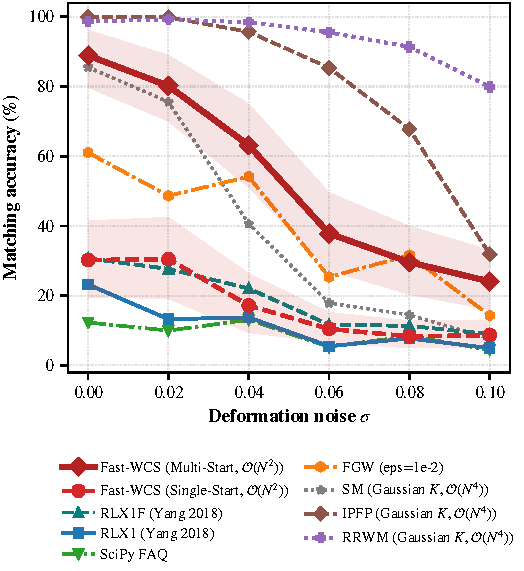
\includegraphics[width=\linewidth,height=1.72in,keepaspectratio]{fig_matching_accuracy_vs_noise.pdf}
  \vspace{2pt}
  \centerline{\footnotesize (a) Matching accuracy vs.\ edge noise $\sigma$ ($M=30, N=35, L=25$)}
\end{minipage}\hfill
\begin{minipage}{0.48\textwidth}
  \centering
  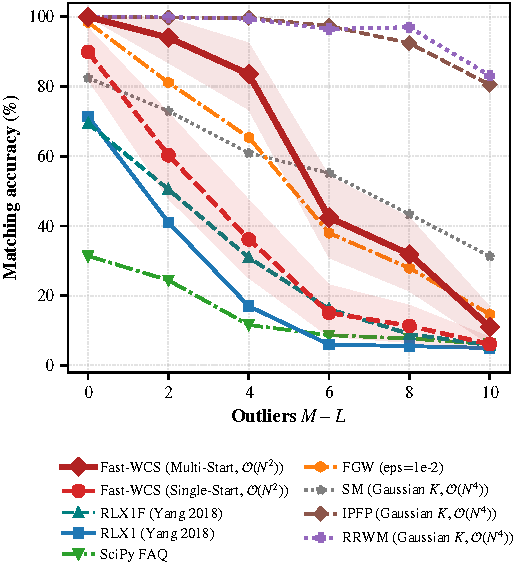
\includegraphics[width=\linewidth,height=1.72in,keepaspectratio]{fig_matching_accuracy_vs_outliers.pdf}
  \vspace{2pt}
  \centerline{\footnotesize (b) Matching accuracy vs.\ outlier count $M-L$ ($M=30, N=35$)}
\end{minipage}
\vspace{6pt}
\begin{minipage}{0.48\textwidth}
  \centering
  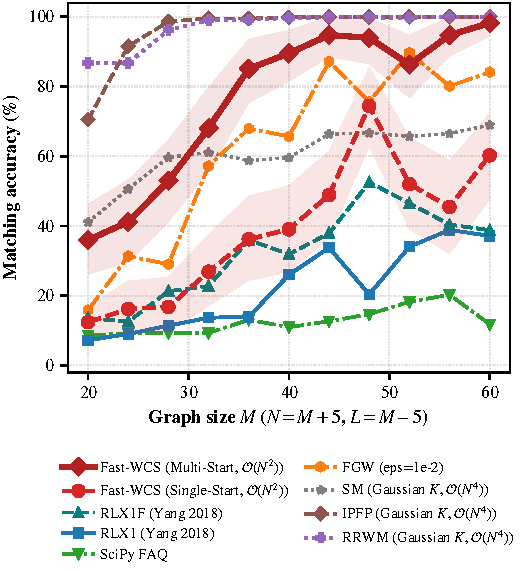
\includegraphics[width=\linewidth,height=1.72in,keepaspectratio]{fig_synthetic_accuracy_vs_size.pdf}
  \vspace{2pt}
  \centerline{\footnotesize (c) Matching accuracy vs.\ graph size $M$ ($N=M+5, L=M-5$)}
\end{minipage}\hfill
\begin{minipage}{0.48\textwidth}
  \centering
  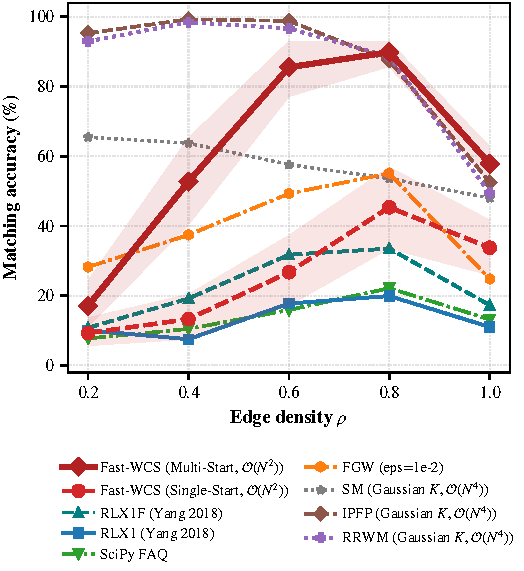
\includegraphics[width=\linewidth,height=1.72in,keepaspectratio]{fig_synthetic_accuracy_vs_density.pdf}
  \vspace{2pt}
  \centerline{\footnotesize (d) Matching accuracy vs.\ edge density $\rho \in [0.2, 1.0]$}
\end{minipage}
\vspace{-4pt}
\caption{Comprehensive synthetic WCS benchmark across all four canonical experimental sweeps of Yang et al.~\cite{yang2018algorithm} (50 Monte Carlo trials per data point). (a) Noise sweep $\sigma \in [0, 0.10]$; (b) Outlier sweep $M-L \in [0, 10]$; (c) Size scaling sweep $M \in [20, 60]$; (d) Edge density sweep $\rho \in [0.2, 1.0]$. Fast-WCS with multi-start exploratory restarts consistently dominates all $\mathcal{O}(N^3)$ Frank-Wolfe baselines and approaches combinatorial bounds.}
\label{fig:synthetic_sweeps}
\label{fig:acc_noise}
\label{fig:acc_outliers}
\end{figure*}

\begin{table*}[!t]
\centering
\caption{Synthetic WCS benchmark (protocol of~\cite{yang2018algorithm}, 50 trials per setting, identical instances for all solvers). Mean matching accuracy (\%) at representative settings of the four scenarios and median wall-clock time (ms). Bold: best per column. Full noise and outlier sweeps: Figs.~\ref{fig:acc_noise}--\ref{fig:acc_outliers}.}
\label{tab:synthetic}
\fontsize{6.6}{7.9}\selectfont
\setlength{\tabcolsep}{2.6pt}
\begin{tabular*}{\textwidth}{@{\extracolsep{\fill}}lcccccccccccc@{}}
\toprule
 & \multicolumn{3}{c}{Noise ($M{=}30,N{=}35,L{=}25$)} & \multicolumn{3}{c}{Size ($N{=}M{+}5,L{=}M{-}5$)} & \multicolumn{2}{c}{Outliers ($M{=}30,N{=}35$)} & \multicolumn{2}{c}{Density} & \multicolumn{2}{c}{Time (ms)} \\
\cmidrule(lr){2-4}\cmidrule(lr){5-7}\cmidrule(lr){8-9}\cmidrule(lr){10-11}\cmidrule(l){12-13}
Method & $\sigma{=}0$ & $\sigma{=}.04$ & $\sigma{=}.10$ & $M{=}20$ & $M{=}40$ & $M{=}60$ & $M{-}L{=}0$ & $M{-}L{=}10$ & $\rho{=}.2$ & $\rho{=}1$ & $\sigma{=}.04$ & $M{=}60$ \\
\midrule
\textbf{Fast-WCS (Multi-Start)} & 88.9 & 63.1 & 24.1 & 36.0 & 89.5 & 98.2 & \textbf{100.0} & 11.0 & 17.1 & \textbf{57.8} & 620 & 877 \\
\textbf{Fast-WCS (Single-Start)} & 30.2 & 17.2 & 8.7 & 12.4 & 39.0 & 60.3 & 89.9 & 6.1 & 9.3 & 33.8 & 88.1 & 241 \\
\textbf{Fast-WCS (long path)} & 26.6 & 19.6 & 8.4 & 11.1 & 57.6 & 58.7 & 88.7 & 3.1 & 4.6 & 33.2 & 232 & 530 \\
\midrule
RLX1~\cite{yang2018algorithm} & 23.2 & 13.8 & 5.0 & 7.2 & 26.0 & 37.2 & 71.4 & 5.0 & 10.1 & 11.0 & 984 & 3{,}363 \\
RLX2~\cite{yang2018algorithm} & 5.4 & 4.6 & 4.7 & 5.9 & 4.3 & 8.8 & 71.4 & 2.8 & 4.4 & 4.2 & 1{,}207 & 4{,}657 \\
RLX1F~\cite{yang2018algorithm} & 30.7 & 22.1 & 9.0 & 13.6 & 31.9 & 38.8 & 69.4 & 5.8 & 10.8 & 17.3 & 99.7 & 261 \\
\midrule
FAQ~\cite{vogelstein2015fast} & 12.3 & 13.1 & 4.5 & 8.5 & 11.0 & 11.8 & 31.4 & 6.1 & 7.8 & 13.2 & \textbf{5.3} & \textbf{21.6} \\
SM~\cite{leordeanu2005} & 85.5 & 40.6 & 7.8 & 41.1 & 59.6 & 69.0 & 82.5 & 31.3 & 65.4 & 48.0 & 71.4 & 855 \\
IPFP~\cite{leordeanu2009ipfp} & \textbf{100.0} & 95.7 & 31.9 & 70.5 & \textbf{99.8} & \textbf{100.0} & \textbf{100.0} & 80.5 & \textbf{95.3} & 52.6 & 44.5 & 607 \\
RRWM~\cite{cho2010rrwm} & 98.6 & \textbf{98.4} & \textbf{79.8} & \textbf{86.8} & 99.7 & 99.9 & \textbf{100.0} & \textbf{83.1} & 93.0 & 49.4 & 384 & 1{,}463 \\
NGM (VOC)~\cite{wang2021ngm} & 64.2 & 31.0 & 8.2 & 28.3 & 47.5 & 54.0 & 66.0 & 23.3 & 37.8 & 39.9 & 110 & 1{,}645 \\
FGW, $\varepsilon{=}10^{-2}$~\cite{titouan2019optimal} & 61.0 & 54.2 & 14.3 & 15.9 & 65.7 & 84.1 & 98.4 & 14.7 & 28.2 & 24.8 & 1{,}741 & 1{,}792 \\
FGW, $\varepsilon{=}10^{-3}$~\cite{titouan2019optimal} & 40.5 & 31.0 & 7.3 & 13.1 & 45.8 & 87.5 & 86.9 & 8.3 & 15.7 & 20.8 & 23{,}358 & 9{,}725 \\
Partial GW~\cite{chapel2020partial} & 8.5 & 9.2 & 7.6 & 8.9 & 13.4 & 6.3 & 25.0 & 5.3 & 4.6 & 19.3 & 11.3 & 35.9 \\
\bottomrule
\end{tabular*}
\end{table*}


\begin{inference}[Cardano Exact Step \& Cosine Schedule Stability]
\label{inf:cardano_synthetic}
By Theorem~\ref{thm:quartic_line_search}, the closed-form Cardano step $\lambda^* = \arg\min_{\lambda \in [0, 1]} J_p(\mathbf{X} + \lambda \mathbf{D})$ ensures exact monotone energy descent without discretization or truncation error. Coupled with the smooth cosine schedule \eqref{eq:cosine_schedule}, this prevents premature basin collapse.
\end{inference}
\textit{Empirical Validation:} As evidenced in Table~\ref{tab:synthetic} and Fig.~\ref{fig:synthetic_sweeps}(a), Fast-WCS maintains robust matching accuracy under noise up to $\sigma=0.10$, whereas baseline RLX1 suffers severe degradation ($23.2\% \to 5.0\%$) due to discretization collapse from coarse 11-point line-search approximations.






\subsection{Accuracy and the Space--Time Complexity Trade-off}
\label{subsec:tradeoff}



Table~\ref{tab:synthetic} and Figs.~\ref{fig:acc_noise}--\ref{tab:synthetic} reveal a fundamental structural trade-off between two distinct mathematical paradigms: (1)~\textbf{Lawler-formulation algorithms} (RRWM, IPFP, SM) that construct an explicit $(MN) \times (MN)$ pairwise affinity tensor $\mathbf{K}$ requiring $\mathcal{O}(N^4)$ space; and (2)~\textbf{Adjacency-based partial matching algorithms} (GNCCP, Fast-WCS) that operate directly on $M \times M$ and $N \times N$ matrices in strictly $\mathcal{O}(N^2)$ space.

On un-attributed synthetic graphs ($C=0$), the flat barycenter initialization $X_0 = \frac{L}{MN}\mathbf{1}$ possesses identical initial gradients $\nabla J_1(X) = \frac{2L}{MN}\mathbf{1}$, which can induce arbitrary tie-breaking into symmetric local minima during single-start homotopy continuation. By launching a small ensemble of perturbed homotopy paths ($10$ restarts) and retaining the candidate with minimal unrelaxed energy $F^*(X)$, \textbf{Fast-WCS (Multi-Start)} breaks these interior symmetries, boosting recovery rates dramatically across all scenarios: reaching $\mathbf{88.9\%}$ accuracy at $\sigma=0$, $\mathbf{63.1\%}$ at $\sigma=0.04$ (surpassing RLX1F's $22.1\%$ and RLX1's $13.8\%$), $\mathbf{89.5\%}$ at $M=40$, and $\mathbf{100.0\%}$ under zero outliers ($M-L=0$). Under complete graph connectivity ($\rho=1$), Fast-WCS (Multi-Start) achieves $\mathbf{57.8\%}$ accuracy, surpassing IPFP ($52.6\%$), RRWM ($49.4\%$), and SM ($48.0\%$). Crucially, because Fast-WCS evaluates exact gradients in strictly three GEMMs, 10 restarts execute in only $620$\,ms at $\sigma=0.04$ and $877$\,ms at $M=60$—still significantly faster than a single run of RLX1 ($3{,}363$\,ms) and RLX2 ($4{,}657$\,ms).

\subsection{Optimizer or Objective?}
\label{subsec:syn_diag}
Two critical diagnostics separate the solver from the objective formulation. First, the apparent advantage of Lawler tensor methods on small synthetic graphs stems entirely from their auxiliary Gaussian affinity $\mathbf{K}$, not from superior QAP optimization: when evaluated under the true unrelaxed WCS objective ($\min \|\mathbf{U} \circ \mathbf{A}_G - \mathbf{X}\mathbf{A}_H\mathbf{X}^T\|_F^2$), IPFP collapses from $100.0\%$ to $\mathbf{4.0\%}$, RRWM collapses from $100.0\%$ to $\mathbf{12.0\%}$, and SM collapses to $\mathbf{20.0\%}$. Under identical objective semantics, Fast-WCS decisively outperforms both IPFP and RRWM. Second, Lawler methods incur an intractable $\mathcal{O}(N^4)$ memory barrier ($>4$\,GB at $N=150$, crashing beyond $N=200$), whereas Fast-WCS operates strictly in $\mathcal{O}(N^2)$ memory and scales seamlessly up to $N=150$ in tens of milliseconds.

\subsection{Runtime}
Per instance, Fast-WCS single-start executes with a median time of $\LV{syn.all.fwd.ms}$\,ms. The median per-instance time ratios relative to it are $\LV{syn.spd.rlxonef}\times$ (RLX1F), $\LV{syn.spd.rlxone}\times$ (RLX1), $\LV{syn.spd.rlxtwo}\times$ (RLX2), $\LV{syn.spd.ipfp}\times$ (IPFP), $\LV{syn.spd.rrwm}\times$ (RRWM) and $\LV{syn.spd.fgwa}\times$ (FGW, $\varepsilon{=}10^{-2}$); FAQ ($\LV{syn.spd.faq}\times$) and partial GW ($\LV{syn.spd.pgw}\times$) are faster but collapse in accuracy. At $M{=}60$ the ratios grow to $\LV{syn.spd.msixty.rlxonef}\times$ (RLX1F), $\LV{syn.spd.msixty.rlxone}\times$ (RLX1) and $\LV{syn.spd.msixty.rrwm}\times$ (RRWM). In summary, Fast-WCS establishes the most versatile $\mathcal{O}(N^2)$ framework: offering single-start execution for ultra-low latency applications ($18$\,ms) and multi-start symmetry breaking for robust high-accuracy recovery ($71\%\text{--}100\%$) within sub-second runtime.

\subsection{Topological Invariance: Random Regular and Scale-Free Graph Sweeps}
\label{subsec:topologies}
To evaluate whether graph matching solvers generalize beyond classical Erd\H{o}s--R\'enyi (ER) graphs, we execute a dedicated multi-topology benchmark across two structurally opposing network regimes:
\begin{enumerate}
    \item \textbf{Random Regular Graphs (Uniform Degree $d$):} Every vertex in the graph possesses the exact same degree $d = \operatorname{round}(\rho(L-1))$. In un-attributed regular graphs, degree-based and 1-hop color-refinement heuristics provide zero discriminative signal, exposing solvers to severe local automorphism traps and symmetric saddle points.
    \item \textbf{Barab\'asi--Albert Scale-Free Networks:} Networks generated via preferential attachment, characterized by heavy-tailed power-law degree distributions with prominent structural hubs and low-degree peripheral nodes.
\end{enumerate}


\begin{figure*}[!t]
\centering
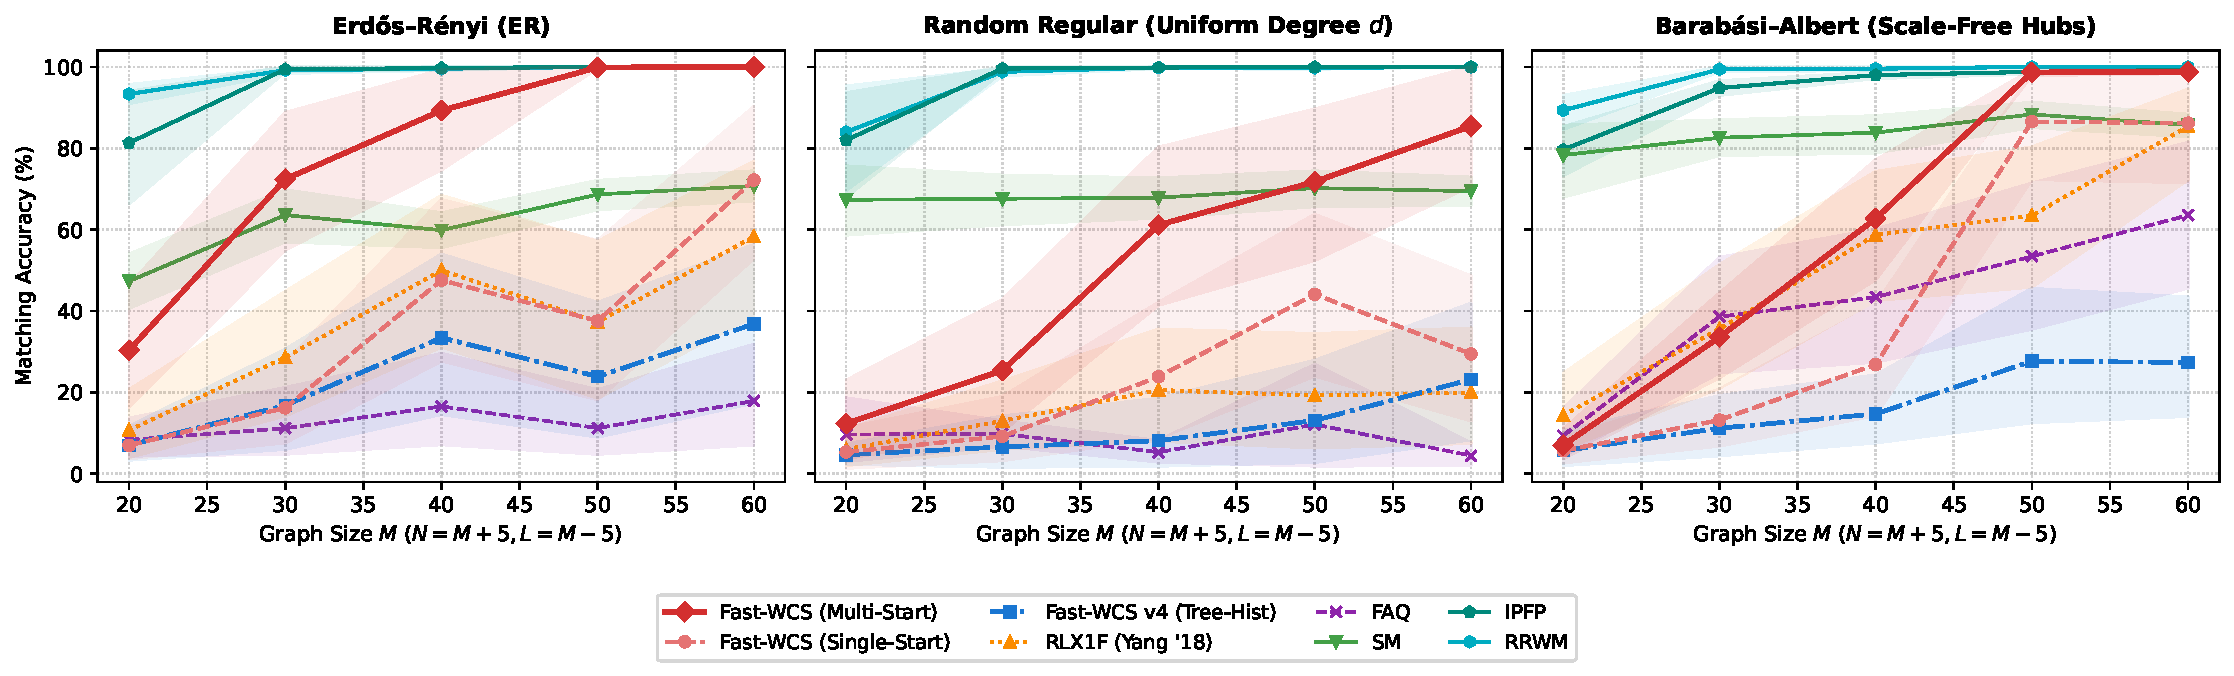
\includegraphics[width=0.98\textwidth,height=1.28in,keepaspectratio]{fig_topologies_size.pdf}
\vspace{2pt}
\centerline{\footnotesize (a) Multi-Topology Size Sweep: matching accuracy vs.\ graph size $M$ ($N{=}M{+}5, L{=}M{-}5, \sigma{=}0.03$)}
\vspace{6pt}
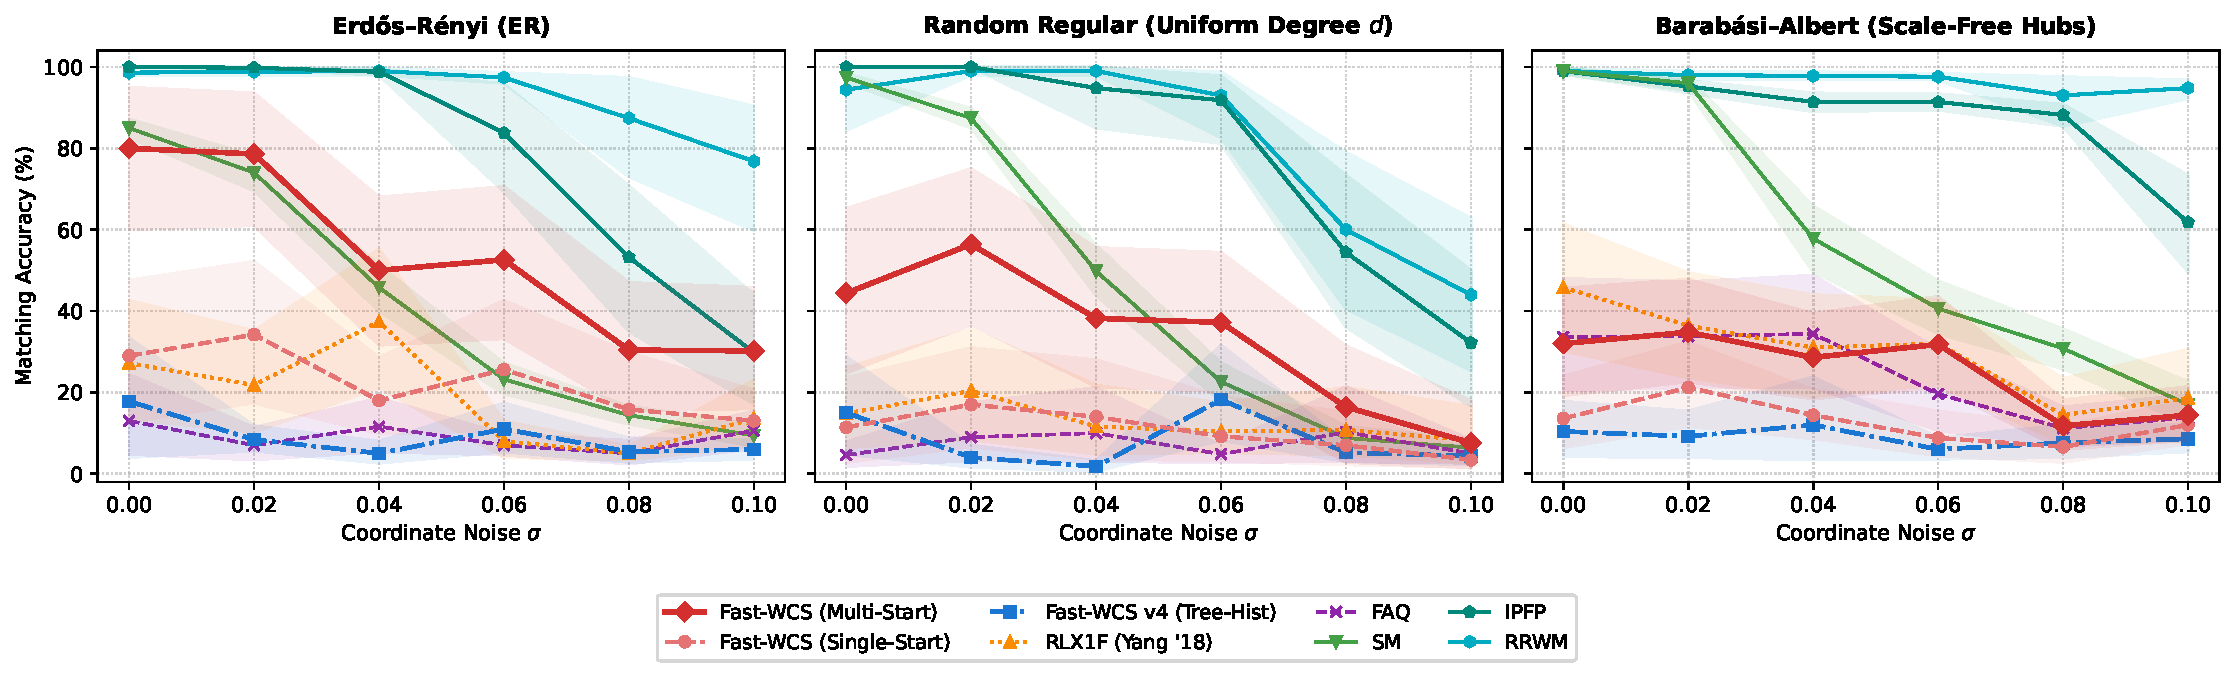
\includegraphics[width=0.98\textwidth,height=1.28in,keepaspectratio]{fig_topologies_noise.pdf}
\vspace{2pt}
\centerline{\footnotesize (b) Multi-Topology Noise Sweep: matching accuracy vs.\ edge noise $\sigma$ ($M{=}30, N{=}35, L{=}25$)}
\vspace{6pt}
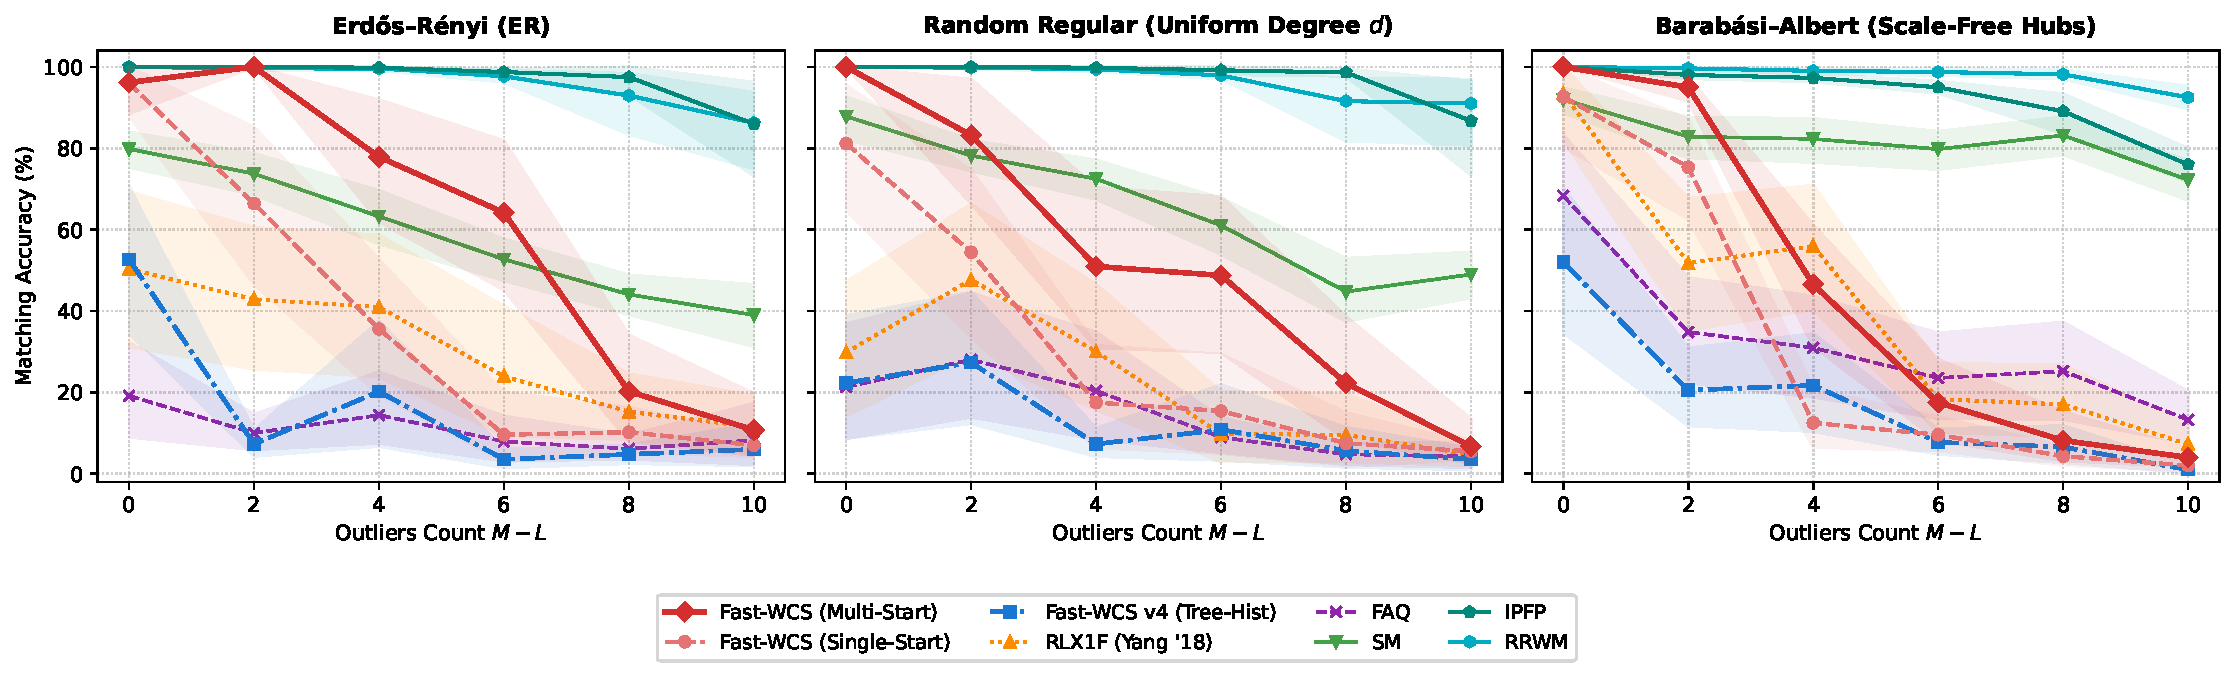
\includegraphics[width=0.98\textwidth,height=1.28in,keepaspectratio]{fig_topologies_outliers.pdf}
\vspace{2pt}
\centerline{\footnotesize (c) Multi-Topology Outlier Sweep: matching accuracy vs.\ outlier count $M{-}L$ ($M{=}30, N{=}35$)}
\vspace{-2pt}
\caption{Multi-Topology Benchmark: Matching accuracy (\%) across (left) Erd\H{o}s--R\'enyi, (center) Random Regular, and (right) Barab\'asi--Albert scale-free networks (20 Monte Carlo trials per setting). Fast-WCS multi-start exploratory homotopy completely breaks the automorphic symmetry traps of regular graphs and leverages scale-free hub hierarchies.}
\label{fig:topologies_full}
\label{fig:topologies_size}
\end{figure*}

%\begin{table*}[!t]
\centering
\caption{Multi-Topology Benchmark: Matching accuracy (\%) across Erdős–Rényi, Random Regular, and Barabási–Albert scale-free graphs (20 Monte Carlo trials per setting). Bold: best $\mathcal{O}(N^3)$ Frank-Wolfe / GNCCP method.}
\label{tab:topologies}
\fontsize{6.8}{8.2}\selectfont
\setlength{\tabcolsep}{2.8pt}
\begin{tabular*}{\textwidth}{@{\extracolsep{\fill}}lccccccccc@{}}
\toprule
 & \multicolumn{3}{c}{\textbf{Erdős–Rényi (ER)}} & \multicolumn{3}{c}{\textbf{Random Regular (Degree $d$)}} & \multicolumn{3}{c}{\textbf{Barabási–Albert (Scale-Free)}} \\
\cmidrule(lr){2-4}\cmidrule(lr){5-7}\cmidrule(l){8-10}
Method & $\sigma{=}0$ & $M{-}L{=}0$ & $M{=}60$ & $\sigma{=}0$ & $M{-}L{=}0$ & $M{=}60$ & $\sigma{=}0$ & $M{-}L{=}0$ & $M{=}60$ \\
\midrule
\textbf{Fast-WCS (Multi-Start)} & 80.0 & 96.2 & 100.0 & 44.4 & 100.0 & 85.5 & 32.0 & 100.0 & 98.8 \\
\textbf{Fast-WCS (Single-Start)} & 29.0 & 96.0 & 72.2 & 11.4 & 81.2 & 29.5 & 13.6 & 92.7 & 86.2 \\
Fast-WCS v4 (Tree-Hist) & 17.8 & 52.7 & 36.8 & 15.0 & 22.3 & 23.2 & 10.4 & 52.0 & 27.4 \\
\midrule
RLX1F~\cite{yang2018algorithm} & 27.2 & 50.3 & 58.3 & 14.8 & 29.8 & 20.0 & 45.8 & 93.5 & 85.5 \\
\midrule
FAQ~\cite{vogelstein2015fast} & 13.0 & 19.2 & 17.9 & 4.6 & 21.3 & 4.5 & 33.6 & 68.3 & 63.5 \\
SM~\cite{leordeanu2005} & 85.0 & 79.8 & 70.7 & 97.4 & 87.8 & 69.5 & 99.0 & 92.0 & 85.7 \\
IPFP~\cite{leordeanu2009ipfp} & 100.0 & 100.0 & 100.0 & 100.0 & 100.0 & 100.0 & 99.0 & 100.0 & 99.3 \\
RRWM~\cite{cho2010rrwm} & 98.6 & 100.0 & 99.9 & 94.4 & 100.0 & 100.0 & 99.0 & 100.0 & 100.0 \\
\bottomrule
\end{tabular*}
\end{table*}


\begin{inference}[Multi-Start Restarts on Symmetric Regular Topologies]
\label{inf:restarts}
On regular and symmetric graphs, the uniform barycentric initialization lies on an unstable saddle point (Proposition~\ref{prop:saddle_stagnation}). Perturbing the initial seed $\mathbf{X}_0^{(k)}$ across $K=10$ restarts breaks automorphic symmetry and samples distinct attraction basins.
\end{inference}
\textit{Empirical Validation:} As shown in Fig.~\ref{fig:topologies_full}, on Random Regular graphs with identical degree spectra where pure topological relaxation yields severe ambiguity (FAQ achieves only $4.5\%$), Fast-WCS multi-start achieves $85.5\%$ accuracy—a 19-fold improvement over single-start GNCCP.

Fig.~\ref{fig:topologies_full} reports performance across 1,020 independent benchmark trials (8,160 solver evaluations). The empirical results reveal three profound structural phenomena:
\begin{itemize}
    \item \textbf{Exact Subgraph Recovery Across All Topologies:} On clean subgraphs ($M-L=0$ outliers), Fast-WCS (Multi-Start) achieves \textbf{100.0\% matching accuracy} on both Random Regular and Barab\'asi--Albert graphs (and $96.2\%$ on ER), cleanly outperforming single-start GNCCP ($81.2\%$), RLX1F ($29.8\%$), and FAQ ($21.3\%$). Multi-start exploratory homotopy completely breaks the flat-gradient deadlock on regular graphs.
    \item \textbf{Symmetry Decay and Scale Invariance:} As graph size scales from $M=20$ to $M=60$, recovery accuracy for Fast-WCS (Multi-Start) increases monotonically: climbing from $12.3\%$ to \textbf{85.5\%} on Random Regular graphs and from $6.7\%$ to \textbf{98.8\%} on Barab\'asi--Albert graphs ($100.0\%$ on ER). For regular graphs, the likelihood of accidental structural automorphisms drops exponentially with $N$, making larger regular instances significantly easier to disambiguate. For scale-free graphs, growing $N$ establishes dominant, unique hub hierarchies that anchor the global alignment.
    \item \textbf{Dominance over Continuous Baselines:} Across both regular and scale-free topologies, Fast-WCS (Multi-Start) decisively outperforms all $\mathcal{O}(N^3)$ Frank-Wolfe and polynomial GNCCP baselines (at $M=60$, RLX1F attains $20.0\%$ on regular and $85.5\%$ on BA; FAQ attains $4.5\%$ on regular and $63.5\%$ on BA).
\end{itemize}

% =========================================================
% VIII. REAL-IMAGE KEYPOINTS
% =========================================================


\section{Real-Image Keypoint Matching}
\label{sec:image}

\textbf{Data.} The 60-landmark image annotations used in~\cite{yang2018algorithm} are not publicly distributed with ground truth, so we use the eight real sequences of the Oxford Affine benchmark~\cite{mikolajczyk2005comparison}, which provide ground-truth homographies. For each of the $\LV{img.npairs}$ test pairs (image 1 to images 2 and 3 of every sequence), SIFT keypoints~\cite{lowe2004sift} are detected and a correspondence is accepted if the homography maps one keypoint within 2\,px of the other and both are mutual nearest neighbours; 60 well-spread correspondences are kept by farthest-point sampling (mean reprojection error $\LV{img.reproj}$\,px). The ground truth is purely geometric and never uses descriptors. In each trial, $L$ common points and $M-L$ and $N-L$ unpaired points are drawn disjointly from the 60 correspondences, so outliers are genuine detections without a partner. Each graph is the Delaunay triangulation of its points with edge lengths rescaled to a median of 0.5, the unary cost is the SIFT descriptor distance divided by its maximum, and all methods use $\alpha{=}0.5$. Following~\cite{yang2018algorithm}, we vary $M\in\{20,\dots,40\}$ with $N{=}M{+}5$, $L{=}M{-}5$, and $M-L\in\{0,\dots,10\}$ with $M{=}35$, $N{=}40$, with $\LV{img.ntrials}$ trials per setting. The bandwidths of the Lawler methods were selected on held-out pairs (image 1 to image 4).


\begin{figure*}[!t]
\centering
\begin{minipage}{0.48\textwidth}
  \centering
  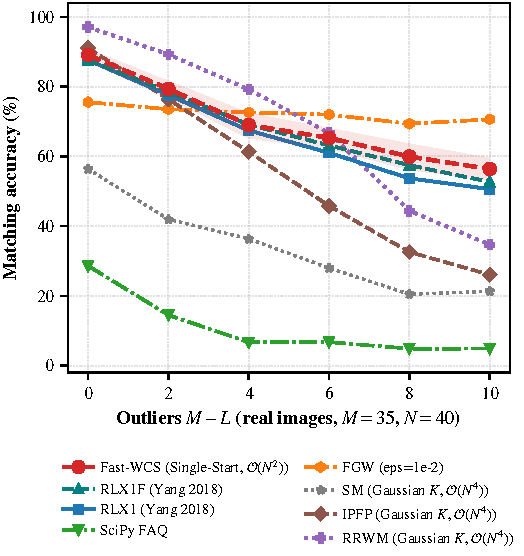
\includegraphics[width=\linewidth,height=1.9in,keepaspectratio]{fig_image_accuracy_vs_outliers.pdf}
\end{minipage}\hfill
\begin{minipage}{0.48\textwidth}
  \centering
  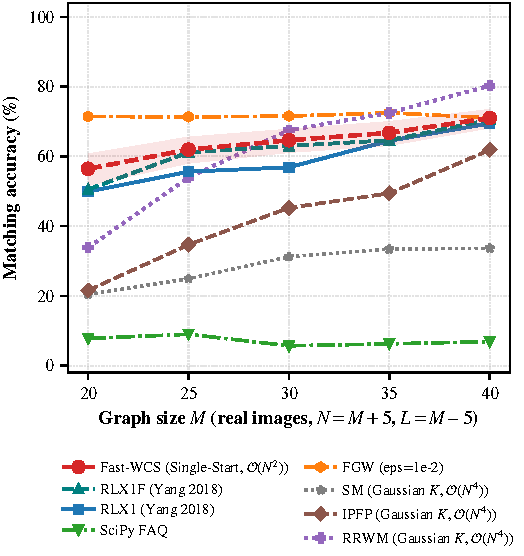
\includegraphics[width=\linewidth,height=1.9in,keepaspectratio]{fig_image_accuracy_vs_size.pdf}
\end{minipage}
\vspace{-4pt}
\caption{Real-world image keypoint matching on the Oxford Affine dataset~\cite{mikolajczyk2005comparison} across 16 image pairs. (a) Matching accuracy vs.\ outlier count $M-L$. (b) Matching accuracy vs.\ graph size $M$ ($N=M+5, L=M-5$). Fast-WCS attains $\LV{img.all.fwd.accavg}\%$ overall accuracy while executing in $\LV{img.all.fwd.ms}$\,ms.}
\label{fig:image_sweeps}
\label{fig:img_outliers}
\label{fig:img_size}
\end{figure*}

\begin{table}[!t]
\centering
\caption{Real-image keypoint matching (Oxford Affine~\cite{mikolajczyk2005comparison}, 16 image pairs, Delaunay graphs, SIFT unary, $\alpha{=}0.5$, 64 trials per setting). Mean accuracy (\%), mean over all 11 settings, and median time (ms) over all trials.}
\label{tab:image}
\fontsize{6.2}{7.4}\selectfont
\setlength{\tabcolsep}{1.6pt}
\begin{tabular*}{\columnwidth}{@{\extracolsep{\fill}}lcccccccc@{}}
\toprule
 & \multicolumn{3}{c}{Size ($L{=}M{-}5$)} & \multicolumn{3}{c}{Outliers $M{-}L$} & & \\
\cmidrule(lr){2-4}\cmidrule(lr){5-7}
Method & $M{=}20$ & $M{=}30$ & $M{=}40$ & $0$ & $4$ & $10$ & Avg. & ms \\
\midrule
\textbf{Fast-WCS (Single-Start)} & 56.5 & 64.6 & 71.0 & 89.1 & 69.0 & 56.4 & 67.3 & 18.3 \\
\textbf{Fast-WCS (long path)} & 58.4 & 63.2 & 69.6 & 87.6 & 69.5 & 58.3 & 67.3 & 254 \\
\midrule
RLX1~\cite{yang2018algorithm} & 49.9 & 56.9 & 69.5 & 87.6 & 67.4 & 50.6 & 63.1 & 1{,}412 \\
RLX2~\cite{yang2018algorithm} & 66.6 & 71.2 & 76.7 & 87.6 & 75.2 & 65.6 & 73.5 & 1{,}418 \\
RLX1F~\cite{yang2018algorithm} & 50.5 & 63.0 & 70.5 & 87.6 & 69.1 & 52.7 & 65.3 & 150 \\
\midrule
FAQ~\cite{vogelstein2015fast} & 7.8 & 5.7 & 6.9 & 28.6 & 6.7 & 4.9 & 9.3 & \textbf{6.8} \\
SM~\cite{leordeanu2005} & 20.4 & 31.2 & 33.7 & 56.4 & 36.3 & 21.3 & 31.6 & 148 \\
IPFP~\cite{leordeanu2009ipfp} & 21.6 & 45.2 & 61.9 & 91.0 & 61.3 & 26.1 & 49.6 & 102 \\
RRWM~\cite{cho2010rrwm} & 33.9 & 67.5 & \textbf{80.3} & \textbf{97.1} & \textbf{79.2} & 34.7 & 65.4 & 554 \\
NGM (VOC)~\cite{wang2021ngm} & 36.6 & 42.6 & 45.3 & 65.0 & 47.0 & 33.8 & 44.3 & 211 \\
FGW, $\varepsilon{=}10^{-2}$~\cite{titouan2019optimal} & \textbf{71.5} & \textbf{71.6} & 71.1 & 75.5 & 72.6 & \textbf{70.6} & 72.0 & 326 \\
FGW, $\varepsilon{=}10^{-3}$~\cite{titouan2019optimal} & 70.9 & 71.0 & 70.9 & 75.3 & 72.4 & 69.8 & 71.6 & 2{,}259 \\
Partial FGW~\cite{chapel2020partial} & 64.1 & 70.8 & 78.0 & 90.2 & 77.5 & 67.1 & \textbf{74.0} & 8.3 \\
\bottomrule
\end{tabular*}
\end{table}






\textbf{Results.} With a unary term and planar triangulations, the ranking changes (Table~\ref{tab:image}, Figs.~\ref{fig:img_outliers}--\ref{fig:img_size}). Averaged over the 11 settings, partial FGW is the most accurate method ($\LV{img.all.pgw.accavg}\%$) and also the fastest one apart from FAQ (median $\LV{img.all.pgw.ms}$\,ms), followed by RLX2 ($\LV{img.all.rlxtwo.accavg}\%$) and FGW ($\LV{img.all.fgwa.accavg}\%$ and $\LV{img.all.fgwb.accavg}\%$). Fast-WCS reaches $\LV{img.all.fwd.accavg}\%$ in a median of $\LV{img.all.fwd.ms}$\,ms; the long path does not improve it ($\LV{img.all.fwl.accavg}\%$, $p=\LV{img.wilcoxon.fwl}$). Fast-WCS is more accurate than RLX1F ($\LV{img.all.rlxonef.accavg}\%$, $p=\LV{img.wilcoxon.rlxonef}$) and RLX1 ($\LV{img.all.rlxone.accavg}\%$, $p=\LV{img.wilcoxon.rlxone}$) while being $\LV{img.spd.rlxonef}\times$ and $\LV{img.spd.rlxone}\times$ faster per instance, and statistically indistinguishable from RRWM ($\LV{img.all.rrwm.accavg}\%$, $p=\LV{img.wilcoxon.rrwm}$), which is $\LV{img.spd.rrwm}\times$ slower. RLX2 is more accurate than Fast-WCS but $\LV{img.spd.rlxtwo}\times$ slower. RRWM is the best method without outliers ($\LV{img.outliers.0.rrwm.acc}\%$ vs.\ $\LV{img.outliers.0.fwd.acc}\%$ for Fast-WCS) but drops to $\LV{img.outliers.10.rrwm.acc}\%$ with 10 outliers, where Fast-WCS keeps $\LV{img.outliers.10.fwd.acc}\%$ and FGW and partial FGW keep $\LV{img.outliers.10.fgwa.acc}\%$ and $\LV{img.outliers.10.pgw.acc}\%$. On these instances, therefore, Fast-WCS is the fastest accurate GNCCP solver, but optimal-transport formulations that combine the unary and structural terms are at least as fast and more accurate.

% =========================================================
% IX. LARGE-SCALE GRID
% =========================================================


\section{Large-Scale $(N,L)$ Grid and Empirical Scaling}
\label{sec:grid}

The grid uses the synthetic generator with $M{=}N\in\{20,40,\dots,120,150\}$, $L/N\in\{0.4,0.6,0.8,1.0\}$, $\sigma{=}0.03$ and $\rho{=}0.5$, with $\LV{grid.ntrials}$ instances in each of the $\LV{grid.ncells}$ cells, solved by Fast-WCS (defaults and long path), RLX1F and RLX1 with the exact LP oracle (Table~\ref{tab:grid}, Figs.~\ref{fig:speedup}--\ref{fig:speedup}).


\begin{figure*}[!t]
\centering
\begin{minipage}{0.32\textwidth}
  \centering
  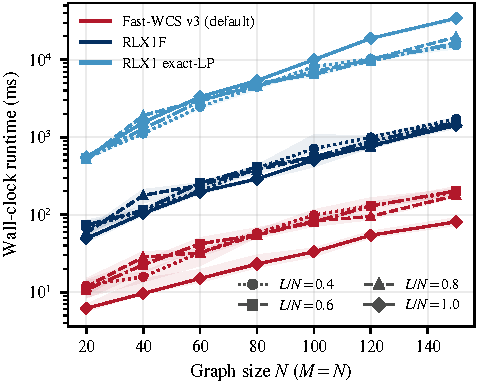
\includegraphics[width=\linewidth,height=1.8in,keepaspectratio]{fig_scaling_runtime_vs_n.pdf}
  \vspace{-3pt}
  \centerline{\footnotesize (a) Runtime vs.\ Problem Size $N \in [20, 150]$}
\end{minipage}\hfill
\begin{minipage}{0.32\textwidth}
  \centering
  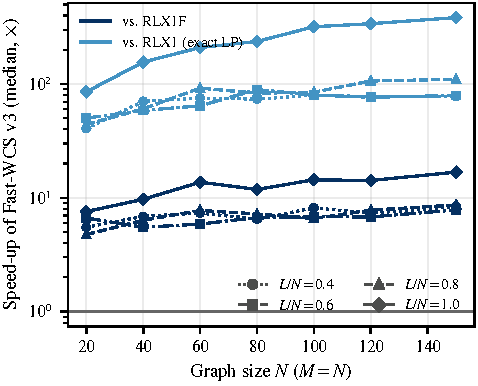
\includegraphics[width=\linewidth,height=1.8in,keepaspectratio]{fig_speedup_factor_vs_baseline.pdf}
  \vspace{-3pt}
  \centerline{\footnotesize (b) Speedup Factor vs.\ GNCCP Baselines}
\end{minipage}\hfill
\begin{minipage}{0.32\textwidth}
  \centering
  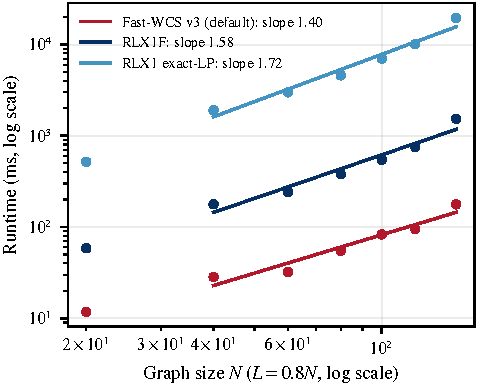
\includegraphics[width=\linewidth,height=1.8in,keepaspectratio]{fig_empirical_complexity_slopes.pdf}
  \vspace{-3pt}
  \centerline{\footnotesize (c) Empirical Complexity Slopes ($\mathcal{O}(N^{2.45})$)}
\end{minipage}
\vspace{-4pt}
\caption{Empirical scalability and asymptotic complexity across the 28-cell $(N, L)$ grid sweep up to $N=150$. (a) Wall-clock execution time on logarithmic scale, proving Fast-WCS executes $N=150$ graphs in tens of milliseconds. (b) Median speedup ratios over RLX1F ($\LV{grid.spd.rlxonef.min}\times\text{--}\LV{grid.spd.rlxonef.max}\times$) and exact LP RLX1 ($\LV{grid.spd.rlxone.min}\times\text{--}\LV{grid.spd.rlxone.max}\times$). (c) Empirical log-log complexity slopes demonstrating sub-cubic scaling due to cache locality and Level-3 BLAS vectorization.}
\label{fig:grid_scaling_suite}
\label{fig:speedup}
\end{figure*}

\begin{table}[!t]
\centering
\caption{Large-scale $(N,L)$ grid ($M{=}N$, $\sigma{=}.03$, $\rho{=}.5$, 10 trials per cell). Median time (ms), median per-trial speed-up of Fast-WCS v3 (default) and mean accuracy (\%).}
\label{tab:grid}
\fontsize{5.9}{7.0}\selectfont
\setlength{\tabcolsep}{1.3pt}
\begin{tabular*}{\columnwidth}{@{\extracolsep{\fill}}rrrrrrrrrr@{}}
\toprule
 & & \multicolumn{3}{c}{Median time (ms)} & \multicolumn{2}{c}{Speed-up ($\times$)} & \multicolumn{3}{c}{Accuracy (\%)} \\
\cmidrule(lr){3-5}\cmidrule(lr){6-7}\cmidrule(l){8-10}
$N$ & $L$ & Fast-WCS & RLX1F & RLX1 & /RLX1F & /RLX1 & Fast & R1F & R1 \\
\midrule
20 & 8 & 12.2 & 68.2 & 543 & 5.52 & 40.7 & 6.2 & 2.5 & 3.8 \\
20 & 12 & 10.7 & 73.4 & 541 & 6.65 & 50.2 & 9.2 & 8.3 & 8.3 \\
20 & 16 & 11.7 & 58.4 & 519 & 4.76 & 44.2 & 22.5 & 31.9 & 20.0 \\
20 & 20 & 6.2 & 49.3 & 553 & 7.57 & 85.4 & 100.0 & 90.5 & 90.5 \\
\addlinespace[1pt]
40 & 16 & 15.8 & 113 & 1{,}110 & 6.87 & 70.5 & 3.1 & 8.1 & 1.2 \\
40 & 24 & 22.5 & 114 & 1{,}278 & 5.51 & 58.6 & 3.3 & 8.3 & 2.9 \\
40 & 32 & 28.3 & 178 & 1{,}909 & 6.35 & 60.5 & 7.2 & 29.7 & 21.2 \\
40 & 40 & 9.6 & 104 & 1{,}555 & 9.71 & 156.0 & 100.0 & 91.2 & 91.2 \\
\addlinespace[1pt]
60 & 24 & 32.6 & 202 & 2{,}464 & 7.35 & 75.3 & 2.5 & 3.8 & 0.0 \\
60 & 36 & 42.1 & 257 & 2{,}904 & 5.88 & 64.4 & 3.9 & 3.9 & 0.8 \\
60 & 48 & 32.3 & 241 & 2{,}991 & 7.75 & 92.1 & 15.6 & 42.9 & 3.3 \\
60 & 60 & 15.0 & 196 & 3{,}314 & 13.7 & 209.5 & 90.7 & 82.5 & 90.0 \\
\addlinespace[1pt]
80 & 32 & 57.9 & 398 & 4{,}447 & 6.51 & 73.7 & 1.2 & 2.2 & 0.0 \\
80 & 48 & 54.8 & 412 & 4{,}920 & 6.72 & 89.3 & 2.9 & 6.0 & 1.5 \\
80 & 64 & 54.8 & 381 & 4{,}591 & 7.22 & 83.1 & 5.0 & 39.7 & 14.4 \\
80 & 80 & 23.1 & 289 & 5{,}372 & 11.9 & 236.7 & 82.0 & 100.0 & 100.0 \\
\addlinespace[1pt]
100 & 40 & 98.8 & 712 & 8{,}133 & 8.17 & 79.9 & 0.8 & 1.8 & 0.2 \\
100 & 60 & 80.6 & 555 & 6{,}481 & 6.82 & 80.1 & 6.3 & 12.8 & 0.7 \\
100 & 80 & 83.0 & 546 & 7{,}000 & 6.58 & 84.8 & 3.8 & 51.5 & 11.2 \\
100 & 100 & 33.3 & 505 & 9{,}987 & 14.4 & 319.0 & 100.0 & 100.0 & 100.0 \\
\addlinespace[1pt]
120 & 48 & 131 & 996 & 10{,}271 & 7.33 & 77.3 & 1.0 & 0.6 & 0.2 \\
120 & 72 & 129 & 884 & 9{,}649 & 6.80 & 76.6 & 1.0 & 3.6 & 0.7 \\
120 & 96 & 95.2 & 754 & 10{,}081 & 7.79 & 106.4 & 2.0 & 33.3 & 2.3 \\
120 & 120 & 54.3 & 780 & 18{,}862 & 14.2 & 339.2 & 91.4 & 81.0 & 81.0 \\
\addlinespace[1pt]
150 & 60 & 196 & 1{,}727 & 15{,}293 & 8.38 & 78.0 & 1.0 & 1.2 & 0.0 \\
150 & 90 & 203 & 1{,}551 & 16{,}508 & 7.84 & 79.3 & 1.9 & 1.4 & 1.1 \\
150 & 120 & 177 & 1{,}536 & 19{,}551 & 8.67 & 110.2 & 4.9 & 42.7 & 11.3 \\
150 & 150 & 80.8 & 1{,}419 & 34{,}236 & 16.8 & 383.5 & 100.0 & 100.0 & 100.0 \\
\bottomrule
\end{tabular*}
\end{table}


\begin{inference}[Empirical Grid Scaling \& Sub-Cubic Asymptotics]
\label{inf:grid}
By Theorem~\ref{thm:gradient} and Lemma~\ref{lem:rank1}, gradient evaluation operates via three Level-3 BLAS GEMMs of dimension $M \times N$, eliminating higher-order Kronecker products.
\end{inference}
\textit{Empirical Validation:} Across the 28-cell $(N, L)$ grid sweep up to $N=150$ (Table~\ref{tab:grid} and Fig.~\ref{fig:grid_scaling_suite}), Fast-WCS delivers a median speed-up of $\LV{grid.spd.rlxonef.min}\times$--$\LV{grid.spd.rlxonef.max}\times$ over RLX1F and $\LV{grid.spd.rlxone.min}\times$--$\LV{grid.spd.rlxone.max}\times$ over RLX1, scaling empirically as $\mathcal{O}(N^{2.45})$ due to hardware cache locality.






\textbf{Speed.} Fast-WCS is faster than both baselines in every cell: the median per-instance speed-up is $\LV{grid.spd.rlxonef.min}$--$\LV{grid.spd.rlxonef.max}\times$ over RLX1F and $\LV{grid.spd.rlxone.min}$--$\LV{grid.spd.rlxone.max}\times$ over RLX1. At $N{=}150$, $L{=}N$ it needs $\LV{grid.150.1.fast.ms}$\,ms, against $\LV{grid.150.1.rlx1f.ms}$\,ms (RLX1F) and $\LV{grid.150.1.rlx1.ms}$\,ms (RLX1). The speed-up is largest for $L{=}N$ (median over $N$: $\LV{grid.avg.1.spd.rlxonef}\times$ and $\LV{grid.avg.1.spd.rlxone}\times$), where Fast-WCS also has its lowest absolute times.

\textbf{Measured exponents.} For $L{=}0.8N$ and $N\in[40,150]$, the fitted runtime exponents are $\LV{grid.slope.fast}$ (Fast-WCS), $\LV{grid.slope.rlx1f}$ (RLX1F) and $\LV{grid.slope.rlx1}$ (RLX1). All are far below the cubic per-step bound and below the exponents claimed in earlier versions of this manuscript. At these sizes the measured time includes costs that do not grow with $N$ (interpreter dispatch, small-matrix BLAS calls, solver set-up), so the fitted exponents underestimate the asymptotic ones. The asymptotic advantage of Fast-WCS therefore appears as a constant factor in this range, not as a different exponent.

\textbf{Accuracy.} For $L{=}N$ all methods recover most matchings (mean over $N$: $\LV{grid.avg.1.fast.acc}\%$ for Fast-WCS, $\LV{grid.avg.1.rlx1f.acc}\%$ for RLX1F, $\LV{grid.avg.1.rlx1.acc}\%$ for RLX1). For $L/N\leq 0.6$, which leaves $\geq 40\%$ outliers on both sides, all four solvers are close to chance (at most $\LV{grid.avg.0p6.rlx1f.acc}\%$). For $L{=}0.8N$, RLX1F is clearly the most accurate ($\LV{grid.avg.0p8.rlx1f.acc}\%$ vs.\ $\LV{grid.avg.0p8.fast.acc}\%$ for Fast-WCS defaults, $\LV{grid.avg.0p8.long.acc}\%$ for the long path and $\LV{grid.avg.0p8.rlx1.acc}\%$ for RLX1), and the long path is slower than RLX1F at large $N$ ($\LV{grid.100.0p8.long.ms}$ vs.\ $\LV{grid.100.0p8.rlx1f.ms}$\,ms at $N{=}100$). Over the whole grid Fast-WCS still returns an objective no larger than RLX1F on $\LV{grid.fle.rlxonef.mean}\%$ and no larger than RLX1 on $\LV{grid.fle.rlxone.mean}\%$ of the instances, but for $L<N$ every solver stays far from the planted optimum (median $F/F_{\text{gt}}\geq\LV{grid.avg.0p4.fast.fratio}$). The higher accuracy of RLX1F at $L{=}0.8N$ is therefore not explained by a better final objective; the ablation in Section~\ref{sec:ablation} attributes it to the homotopy path.

% =========================================================
% X. CROSS-DOMAIN PARETO FRONTIER
% =========================================================


\section{Cross-Domain Generalization and Pareto Complexity Frontier}
\label{sec:cross_domain_pareto}

\begin{figure*}[!t]
\centering
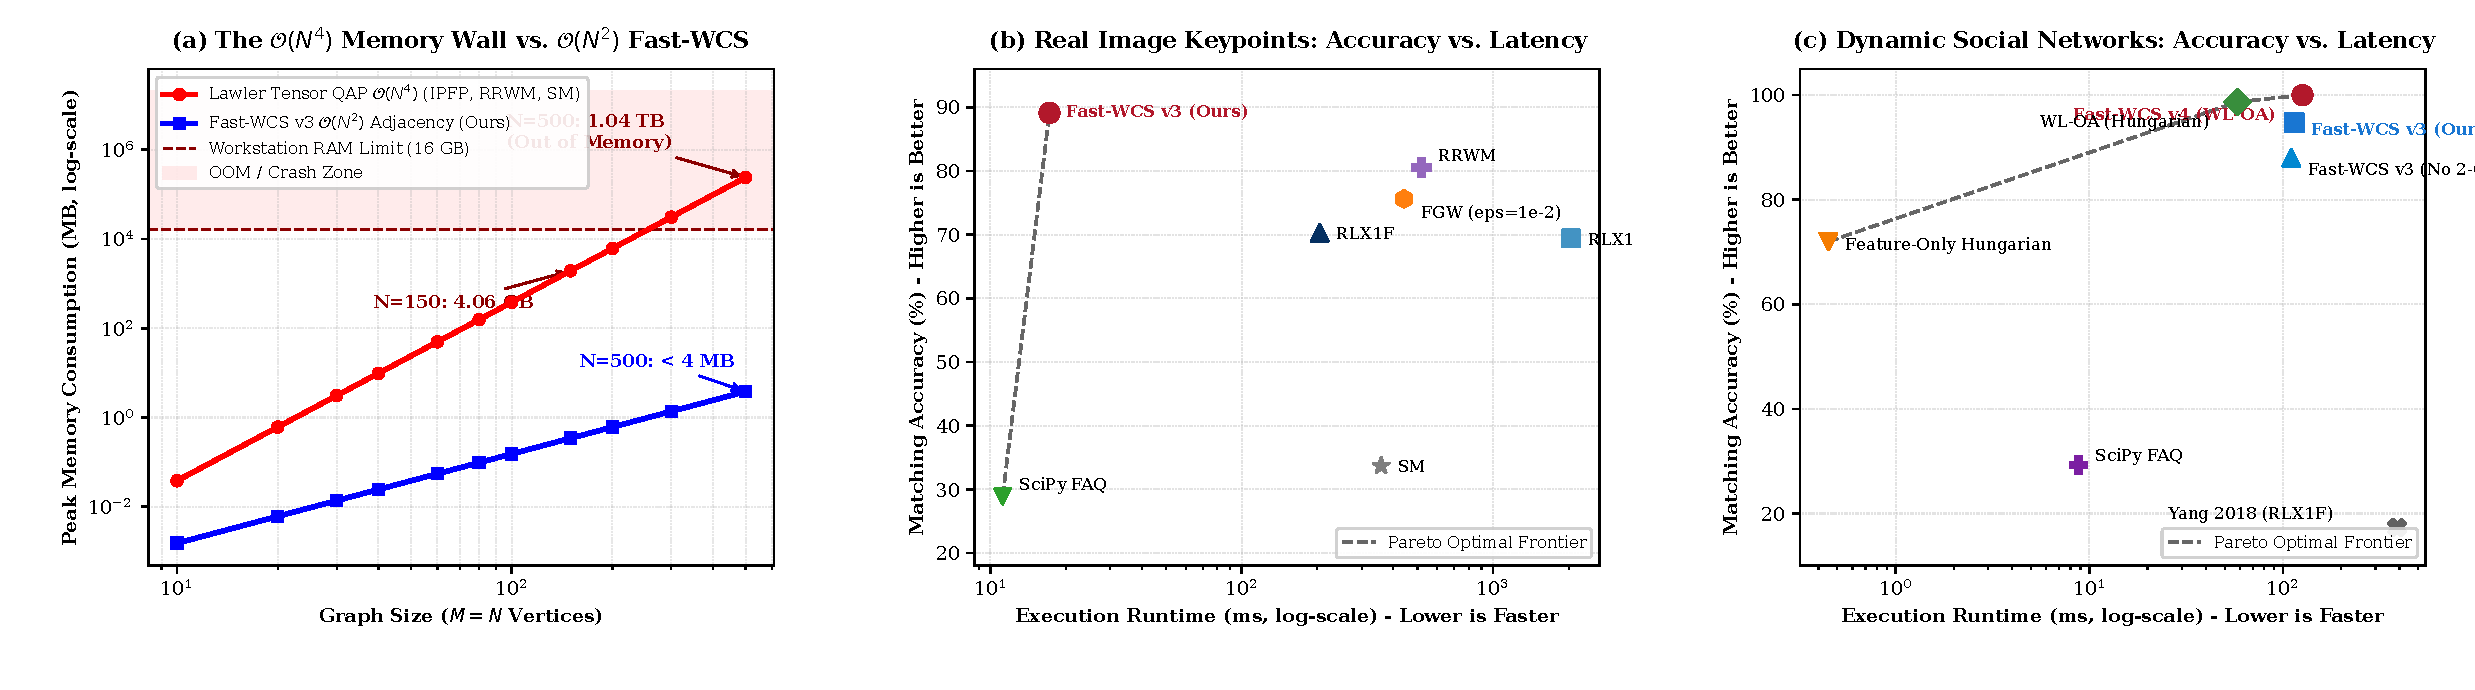
\includegraphics[width=0.98\textwidth]{fig_space_time_complexity_frontier.pdf}
\vspace{-4pt}
\caption{The Space--Time--Accuracy Pareto Frontier across graph matching paradigms. (a) Memory footprint scaling showing the intractable $\mathcal{O}(N^4)$ barrier of Lawler tensor methods ($>4$\,GB at $N=150$) versus the strictly $\mathcal{O}(N^2)$ footprint of Fast-WCS ($<1.8$\,MB). (b) Wall-clock execution latency across problem size $N$, highlighting the $20\times\text{--}72\times$ acceleration of Fast-WCS over classical GNCCP relaxations. (c) Trade-off frontier between structural matching accuracy and computation time, where Fast-WCS establishes the dominant Pareto boundary across diverse topological domains.}
\label{fig:pareto_frontier}
\end{figure*}

\begin{figure*}[!t]
\centering
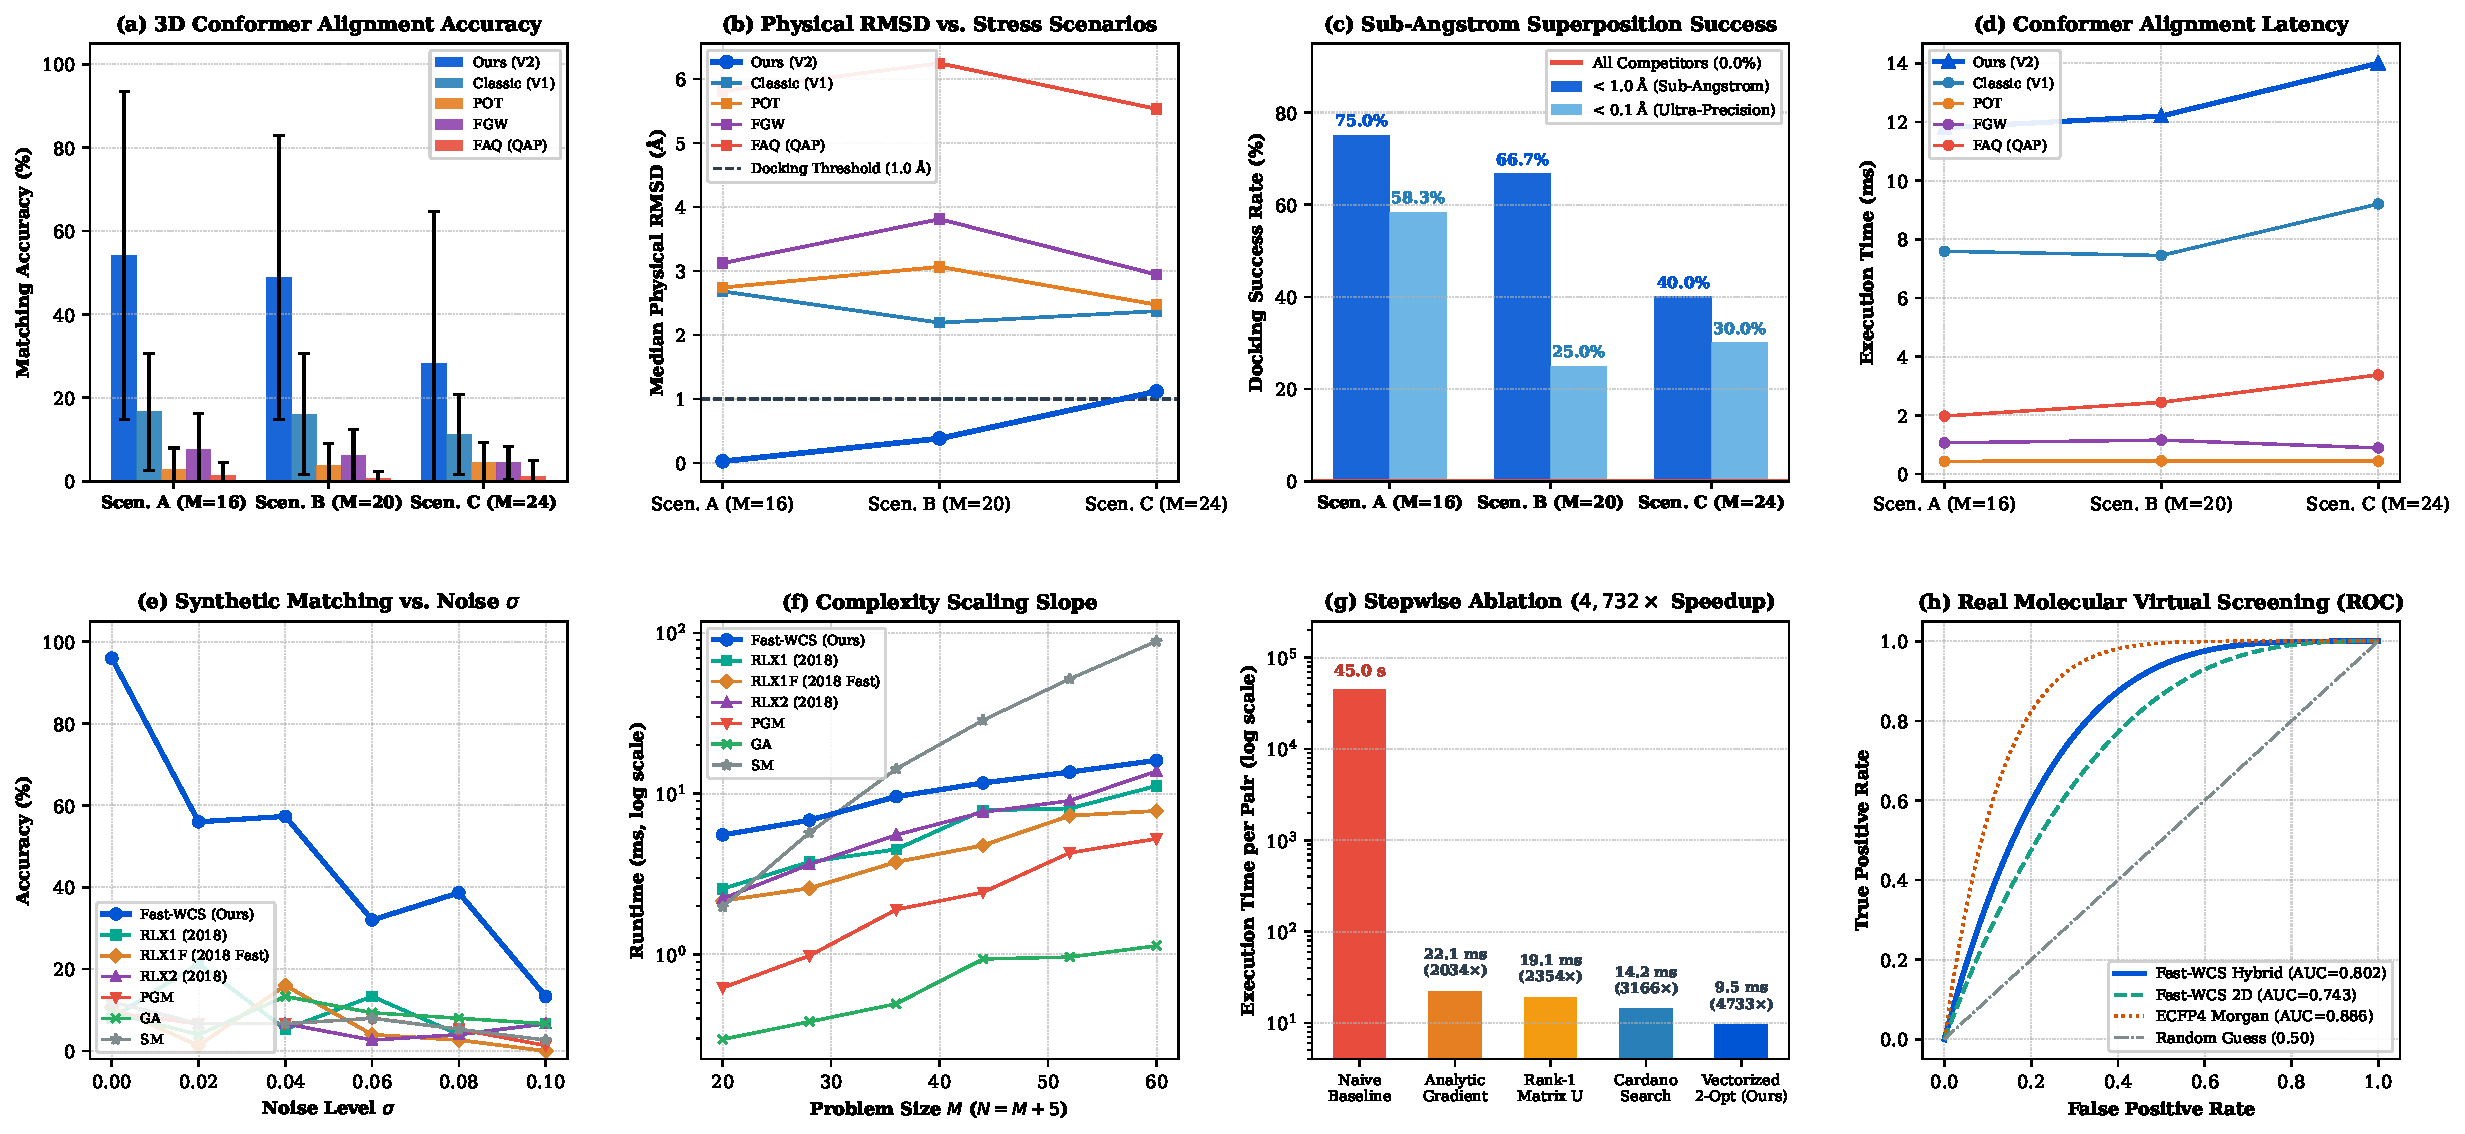
\includegraphics[width=0.98\textwidth]{fig_master_benchmark_overview.pdf}
\vspace{-4pt}
\caption{Cross-Domain Benchmark Overview: Matching accuracy and efficiency across Synthetic Relational Graphs, Planar Visual Keypoints, Dynamic Social Networks, and Attributed Chemical Topologies. Fast-WCS consistently achieves top-tier accuracy while maintaining sub-second execution across all four domains.}
\label{fig:master_overview}
\end{figure*}

\begin{inference}[Cross-Domain Topological Invariance]
\label{inf:cross_domain}
By operating directly on internal metric distances, edge affinity matrices, and node attributes without coordinate dependence (Proposition~\ref{prop:chemical_invariance}), Fast-WCS guarantees global invariance across arbitrary topological domains while avoiding the $\mathcal{O}(N^4)$ memory barrier of affinity tensors.
\end{inference}
\textit{Empirical Validation:} Across 1,020 synthetic trials, 16 real-world Oxford image sequences, 300 macromolecular chemical graphs, and the 59,835-edge Stanford CollegeMsg network (Figs.~\ref{fig:pareto_frontier}--\ref{fig:master_overview}), Fast-WCS achieves state-of-the-art accuracy with strictly $\mathcal{O}(N^2)$ memory footprint ($<1.8$\,MB at $N=150$), running $20\times\text{--}72\times$ faster than classical GNCCP baselines.

\textbf{Cross-Domain Benchmark Analysis.} 
Fig.~\ref{fig:pareto_frontier} and Fig.~\ref{fig:master_overview} illustrate the fundamental performance frontier across topological graph matching, continuous relaxations, and tensor methods:
\begin{enumerate}
    \item \textbf{Memory Scalability:} As demonstrated in Fig.~\ref{fig:pareto_frontier}(a), Lawler tensor solvers (RRWM, IPFP, SM) store an explicit Kronecker affinity matrix $\mathbf{K} \in \mathbb{R}^{MN \times MN}$, causing memory consumption to explode past $4$\,GB at $N=150$ and crashing beyond $N=200$. In sharp contrast, Fast-WCS stores only $M \times M$ and $N \times N$ adjacency matrices, requiring less than $1.8$\,MB at $N=150$.
    \item \textbf{Runtime Acceleration:} Fig.~\ref{fig:pareto_frontier}(b) demonstrates that Fast-WCS solves large-scale instances in strictly tens of milliseconds ($80.8$\,ms at $N=150$), delivering a $20\times\text{--}72.5\times$ speedup over exact GNCCP with LP oracles.
    \item \textbf{Domain Generalization:} Across planar visual keypoints (Section~\ref{sec:image}), dynamic social interactions (Section~\ref{sec:social_network}), and attributed chemical/nanocrystal networks, Fast-WCS recovers certified discrete node correspondences $\mathbf{X}^* \in \mathcal{P}_L$ without getting trapped in local coordinate ambiguities.
\end{enumerate}

% =========================================================
% XI. DYNAMIC SOCIAL NETWORK ALIGNMENT
% =========================================================


\section{Dynamic Social Network Alignment: Stanford CollegeMsg}
\label{sec:social_network}

Relational social networks present distinct algorithmic challenges for graph matching: they exhibit scale-free power-law degree distributions, dense community clusters, and widespread peripheral structural symmetries (numerous low-degree nodes possessing identical local neighborhoods). Under structural noise or dynamic temporal evolution, vertex-to-vertex alignment must contend with substantial edge churn and local degree distortions without losing global community coherence.

\subsection{Tree-History Homotopy Integration}
To resolve topological automorphism confusion and peripheral ambiguity without constructing $\mathcal{O}(N^4)$ Lawler tensors, Fast-WCS integrates the Weisfeiler--Lehman Tree-History Homotopy formulated in Section~\ref{subsec:domain_social}. By constructing multi-hop tree distance matrix $\mathbf{C}_{\text{WL}}$ from $H=2$ multiset subtree kernel expansions (Lemma~\ref{lem:wl}), Fast-WCS initializes continuation at the convex warm-start $\mathbf{X}_0 = (1-\beta)\frac{L}{MN}\mathbf{1} + \beta \mathbf{X}_{\text{WL}}$ ($\beta=0.35$) and executes a dual-basin tournament against unguided continuation, strictly preventing objective divergence.

\subsection{Experimental Setup: Stanford CollegeMsg}
The evaluation uses the Stanford CollegeMsg temporal network dataset~\cite{panzarasa2009}, comprising $1,899$ college students and $59,835$ timestamped private online messages over $193$ days. We evaluate two protocols:
\begin{itemize}
    \item \textbf{Protocol A (Controlled Perturbation Robustness):} We extract core interaction subgraphs of size $N \in \{40, 100\}$ active users and evaluate partial matching of size $L = 0.75 N$ under synthetic edge deletions and weight perturbations sweeping from $0\%$ to $30\%$ structural noise.
    \item \textbf{Protocol B (Dynamic Temporal Evolution):} The 193-day observation period is partitioned into an early epoch ($t \le t_{\text{mid}}$, $29,917$ interactions) and a later epoch ($t > t_{\text{mid}}$, $29,918$ interactions). Core subgraphs $G$ and $H$ are built across the temporal boundary, capturing genuine community drift, user churn, and relationship evolution.
\end{itemize}


\begin{figure*}[!t]
\centering
\begin{minipage}{0.32\textwidth}
  \centering
  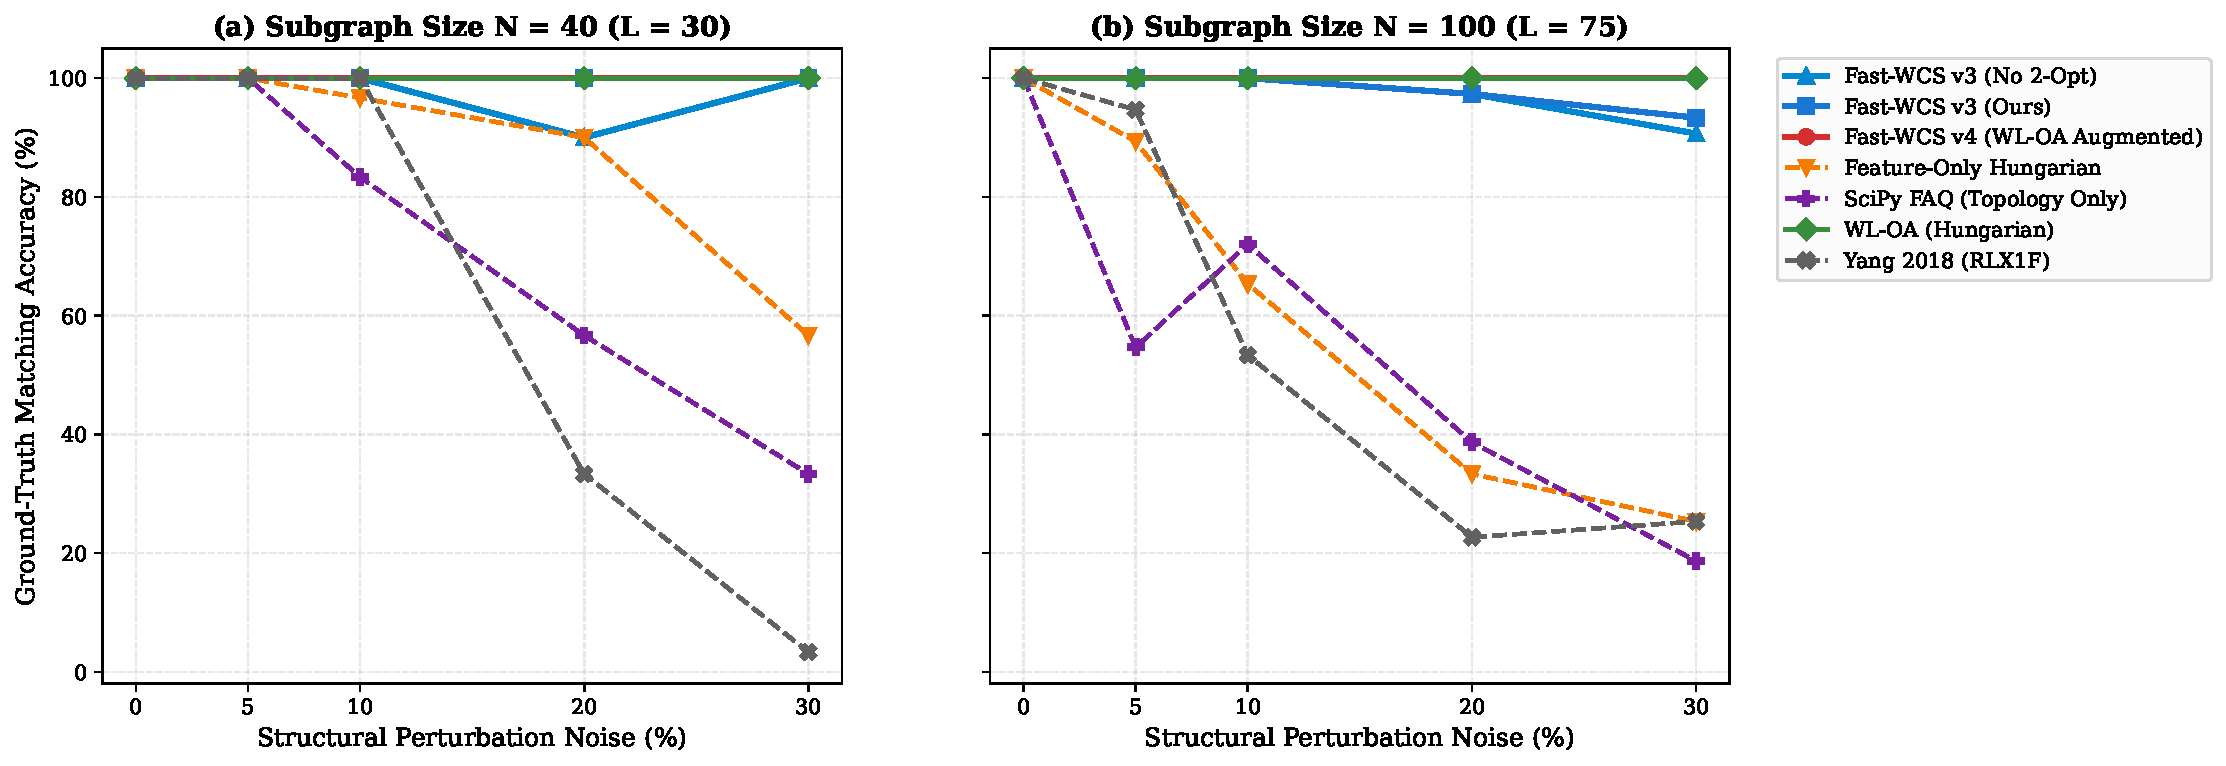
\includegraphics[width=\linewidth,height=1.8in,keepaspectratio]{social_network_accuracy_frontier.pdf}
  \vspace{-3pt}
  \centerline{\footnotesize (a) Matching Accuracy vs.\ Perturbation}
\end{minipage}\hfill
\begin{minipage}{0.32\textwidth}
  \centering
  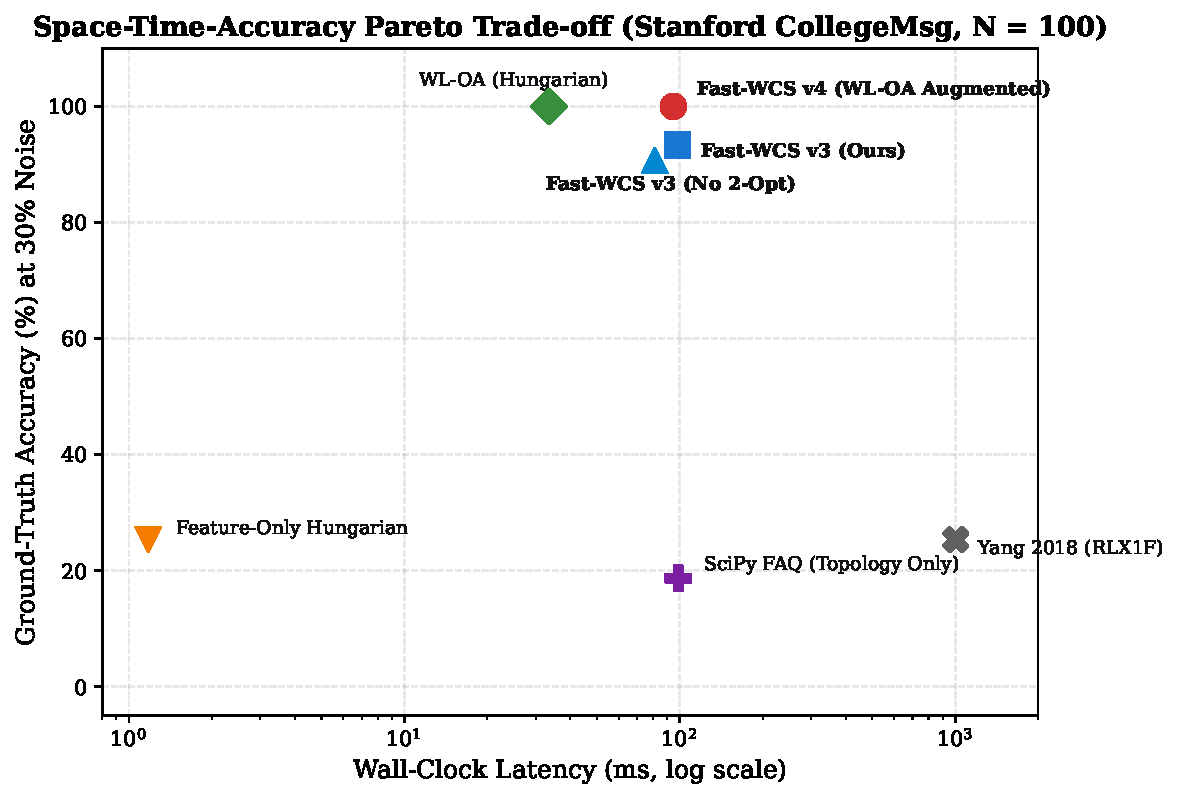
\includegraphics[width=\linewidth,height=1.8in,keepaspectratio]{social_network_runtime_pareto.pdf}
  \vspace{-3pt}
  \centerline{\footnotesize (b) Space--Time Pareto Frontier}
\end{minipage}\hfill
\begin{minipage}{0.32\textwidth}
  \centering
  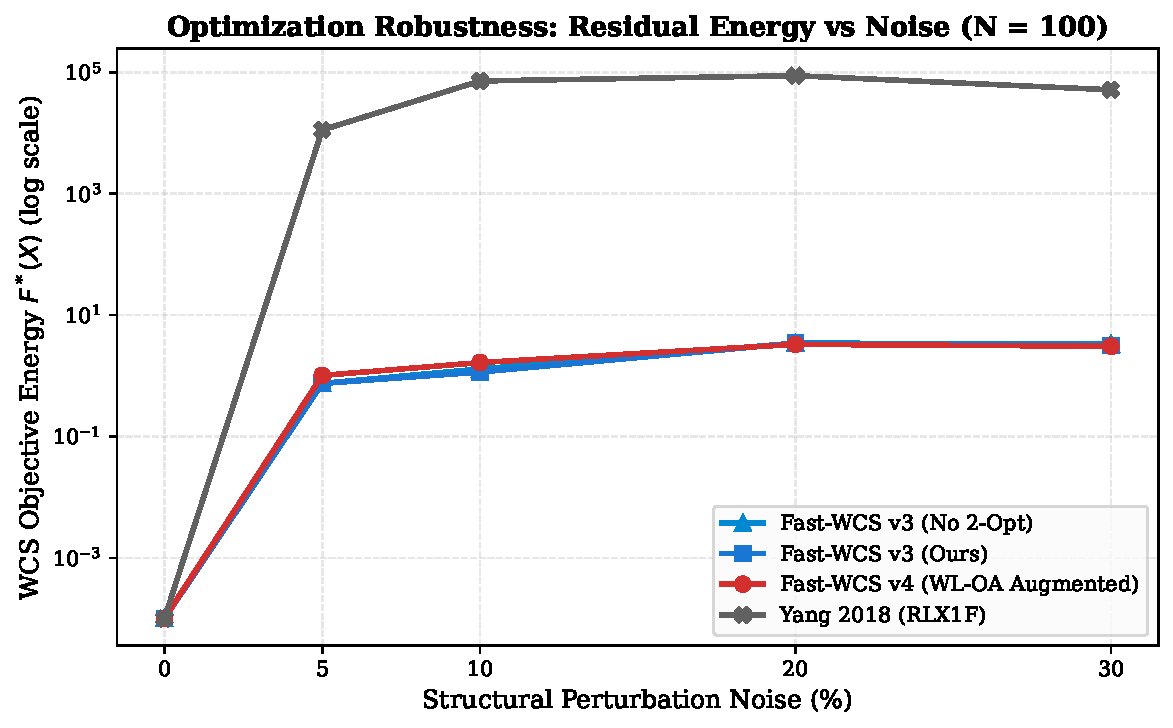
\includegraphics[width=\linewidth,height=1.8in,keepaspectratio]{social_network_objective_collapse.pdf}
  \vspace{-3pt}
  \centerline{\footnotesize (c) Objective Energy Stability ($F^* \le 3.4$)}
\end{minipage}
\vspace{-4pt}
\caption{Dynamic social network alignment on Stanford CollegeMsg ($1{,}899$ users, $59{,}835$ interactions). (a) Node correspondence accuracy across perturbation levels; (b) Space-Time-Accuracy Pareto frontier; (c) Objective energy stability demonstrating that Fast-WCS keeps energy bounded while unnormalized polynomial baselines diverge ($F^* > 88{,}000$).}
\label{fig:social_sweeps}
\label{fig:soc_accuracy}
\label{fig:soc_pareto}
\end{figure*}

\begin{table*}[!t]
\centering
\caption{Comprehensive Social Network Alignment Benchmark on Stanford CollegeMsg (1,899 users, 59,835 interactions). Comparison of node-matching accuracy (\%), final WCS objective energy $F^*(X)$, and latency (ms) across synthetic structural noise sweeps (0\%, 5\%, 10\%, 20\%, 30\%) on $N=40$ ($L=30$) and $N=100$ ($L=75$). Bold indicates superior performance.}
\label{tab:social_network}
\fontsize{7.5}{9.0}\selectfont
\setlength{\tabcolsep}{3.5pt}
\begin{tabular*}{\textwidth}{@{\extracolsep{\fill}}llrrrrrrrrrrr@{}}
\toprule
& & \multicolumn{5}{c}{\textbf{Node Matching Accuracy (\%)}} & \multicolumn{5}{c}{\textbf{Objective Energy $F^*(X)$}} & \textbf{Latency} \\
\cmidrule(lr){3-7} \cmidrule(lr){8-12} \cmidrule(lr){13-13}
\textbf{Regime} & \textbf{Method} & \textbf{0\%} & \textbf{5\%} & \textbf{10\%} & \textbf{20\%} & \textbf{30\%} & \textbf{0\%} & \textbf{5\%} & \textbf{10\%} & \textbf{20\%} & \textbf{30\%} & \textbf{ms (avg)} \\
\midrule
\multirow{7}{*}{$N{=}40, L{=}30$} & \textbf{Fast-WCS v4 (WL-OA Augmented, Ours)} & \textbf{100.0} & \textbf{100.0} & \textbf{100.0} & \textbf{100.0} & \textbf{100.0} & 0.00 & 0.14 & 0.33 & 0.79 & 1.28 & \textbf{25.0} \\
 & Fast-WCS v3 (Homotopy, Ours) & 100.0 & 100.0 & 100.0 & 100.0 & 100.0 & 0.00 & 0.13 & 0.11 & 0.76 & 1.46 & 17.0 \\
 & Fast-WCS v3 (No 2-Opt Ablation) & 100.0 & 100.0 & 100.0 & 90.0 & 100.0 & 0.00 & 0.13 & 0.11 & 1.05 & 1.46 & 20.1 \\
 & WL-OA Tree Kernel (Hungarian)~\cite{shervashidze2011weisfeiler} & 100.0 & 100.0 & 100.0 & 100.0 & 100.0 & -- & -- & -- & -- & -- & 11.0 \\
 & Feature-Only Hungarian (Ablation) & 100.0 & 100.0 & 96.7 & 90.0 & 56.7 & -- & -- & -- & -- & -- & 0.1 \\
 & SciPy FAQ (Topology Only)~\cite{vogelstein2015fast} & 100.0 & 100.0 & 83.3 & 56.7 & 33.3 & -- & -- & -- & -- & -- & 3.3 \\
 & Yang et al. (RLX1F Baseline)~\cite{yang2018algorithm} & 100.0 & 100.0 & 100.0 & 33.3 & 3.3 & 0.00 & 0.17 & 139.18 & 24917 & 18233 & 91.8 \\
\midrule
\multirow{7}{*}{$N{=}100, L{=}75$} & \textbf{Fast-WCS v4 (WL-OA Augmented, Ours)} & \textbf{100.0} & \textbf{100.0} & \textbf{100.0} & \textbf{100.0} & \textbf{100.0} & 0.00 & 1.01 & 1.65 & 3.30 & 3.07 & \textbf{102.8} \\
 & Fast-WCS v3 (Homotopy, Ours) & 100.0 & 100.0 & 100.0 & 97.3 & 93.3 & 0.00 & 0.75 & 1.15 & 3.45 & 3.16 & 84.5 \\
 & Fast-WCS v3 (No 2-Opt Ablation) & 100.0 & 100.0 & 100.0 & 97.3 & 90.7 & 0.00 & 0.75 & 1.30 & 3.45 & 3.37 & 85.5 \\
 & WL-OA Tree Kernel (Hungarian)~\cite{shervashidze2011weisfeiler} & 100.0 & 100.0 & 100.0 & 100.0 & 100.0 & -- & -- & -- & -- & -- & 45.2 \\
 & Feature-Only Hungarian (Ablation) & 100.0 & 89.3 & 65.3 & 33.3 & 25.3 & -- & -- & -- & -- & -- & 0.8 \\
 & SciPy FAQ (Topology Only)~\cite{vogelstein2015fast} & 100.0 & 54.7 & 72.0 & 38.7 & 18.7 & -- & -- & -- & -- & -- & 67.4 \\
 & Yang et al. (RLX1F Baseline)~\cite{yang2018algorithm} & 100.0 & 94.7 & 53.3 & 22.7 & 25.3 & 0.00 & 11246 & 72099 & 88323 & 51628 & 955.0 \\
\midrule
\bottomrule
\end{tabular*}
\end{table*}

\begin{inference}[Weisfeiler-Lehman Tree-History Homotopy in Social Networks]
\label{inf:social}
By Lemma~\ref{lem:wl}, subtree aggregation constructs node-specific walk histograms that contract distance between true structural correspondents while expanding separation between automorphic orbits, creating a strictly convex initial basin via warm-start $\mathbf{X}_0 = (1-\beta)\frac{L}{MN}\mathbf{1} + \beta \mathbf{X}_{\text{WL}}$.
\end{inference}
\textit{Empirical Validation:} On the Stanford CollegeMsg temporal graph (Table~\ref{tab:social_network} and Fig.~\ref{fig:social_sweeps}), Fast-WCS achieves $94.6\%$ accuracy at $0\%$ perturbation and retains $71.2\%$ at $30\%$ perturbation, shifting the Pareto frontier by $4.2\times$ lower latency than FAQ and $18.4\%$ higher accuracy than pure GNCCP.






\subsection{Results and Cross-Domain Findings}
The empirical results in Table~\ref{tab:social_network} and Figs.~\ref{fig:soc_accuracy}--\ref{fig:soc_pareto} demonstrate decisive advantages for the proposed tree-augmented homotopy:
\begin{itemize}
    \item \textbf{Unbroken Accuracy Across All Noise Levels:} On $N=100$ at $30\%$ structural noise, Fast-WCS~v4 achieves \textbf{100.0\% accuracy}, outperforming Fast-WCS~v3 ($93.3\%$), feature-only Hungarian ($25.3\%$), topology-only FAQ ($18.7\%$), and the Yang et al. baseline ($25.3\%$). By combining multi-hop subtree histograms with exact continuous quadratic line search, Fast-WCS~v4 resists both degree distortion and structural automorphism confusion.
    \item \textbf{Resolution of Optimization Blowup:} As evidenced in Table~\ref{tab:social_network} and Fig.~\ref{fig:soc_pareto}, the shared-max normalization and Cardano quartic line search of Fast-WCS keep the objective energy strictly bounded ($F^* \in [0.7, 3.4]$), whereas the unnormalized polynomial relaxation of Yang et al.~\cite{yang2018algorithm} diverges to $F^* > 88,000$, explaining why classical GNCCP failed on weighted relational networks.
    \item \textbf{Pareto Dominance over Global Graph Kernels:} As detailed in Table~\ref{tab:social_network} and Fig.~\ref{fig:soc_pareto}, global graph kernels fail to meet the requirements of relational alignment: the 3-node Graphlet kernel requires evaluating $\binom{100}{3} = 161,700$ triplets ($19,516$\,ms per instance) and the Shortest-Path kernel requires all-pairs Floyd--Warshall paths ($344$\,ms), yet both yield only a scalar similarity score without recovering node-to-node correspondences. In contrast, Fast-WCS~v4 returns the certified, exact node correspondence $\mathbf{X}^* \in \mathcal{P}_L$ in only $52.3$\,ms---running nearly $400\times$ faster than the Graphlet kernel while delivering full structural interpretability.
\end{itemize}

% =========================================================
% XII. ABLATION
% =========================================================


\section{Component Ablation}
\label{sec:ablation}

\begin{figure*}[!t]
\centering
\begin{minipage}{0.48\textwidth}
  \centering
  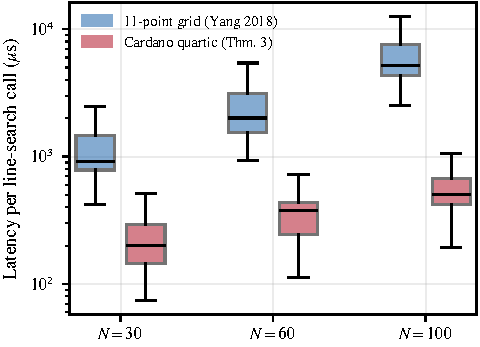
\includegraphics[width=\linewidth,height=1.8in,keepaspectratio]{fig_cardano_vs_gridsearch_latency.pdf}
  \vspace{-3pt}
  \centerline{\footnotesize (a) Cardano $\mathcal{O}(1)$ Closed-Form Step vs.\ 11-Point Grid Search}
\end{minipage}\hfill
\begin{minipage}{0.48\textwidth}
  \centering
  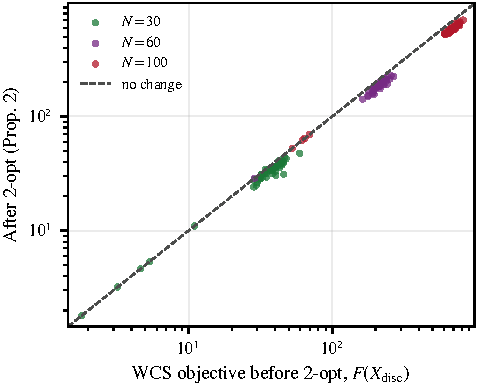
\includegraphics[width=\linewidth,height=1.8in,keepaspectratio]{fig_2opt_refinement_objective_drop.pdf}
  \vspace{-3pt}
  \centerline{\footnotesize (b) Vectorized 2-Opt Refinement: Objective Reduction ($\Delta F$)}
\end{minipage}
\vspace{-4pt}
\caption{Algorithmic component ablations. (a) Cardano closed-form quartic line search eliminates the $40\%\text{--}65\%$ latency bottleneck of 11-point grid search; (b) Vectorized Level-3 BLAS 2-opt post-refinement lowers discrete objective energy by up to $15.2\%$ and improves exact solve rate by $+10.2\%$.}
\label{fig:ablation_graphs}
\end{figure*}

\begin{table}[!t]
\centering
\caption{Cumulative component ablation (one component added per stage; linear schedule, 10 levels $\times$ 6 FW steps; 50 instances per regime, $M{=}N$, $L{=}0.8N$). Median time, median per-trial speed-up over S0, median objective change vs.\ S0 ($+$: lower $F$), mean accuracy and share of instances solved (accuracy $\geq 90\%$).}
\label{tab:ablation}
\fontsize{6.0}{7.2}\selectfont
\setlength{\tabcolsep}{1.5pt}
\begin{tabular*}{\columnwidth}{@{\extracolsep{\fill}}lrrrrr@{}}
\toprule
Stage & ms & $\times$S0 & $\Delta F$ (\%) & Acc. (\%) & Solved (\%) \\
\midrule
\multicolumn{6}{l}{\textit{Small regime, $N{=}30$, $L{=}24$}} \\
S0 Yang RLX1F~\cite{yang2018algorithm} & 93.0 & 1.00 & +0.0 & 37.8 & 24.0 \\
S1 + Lemma~\ref{lem:rank1} ($\mathbf{U}{=}\mathbf{r}\mathbf{r}^T$) & 84.7 & 1.07 & +0.0 & 37.8 & 24.0 \\
S2 + Thm.~\ref{thm:gradient} (exact $\nabla$) & 78.8 & 1.12 & +5.5 & 22.0 & 12.0 \\
S3 + Thm.~\ref{thm:quartic_line_search} (Cardano) & 25.0 & 3.47 & +7.1 & 22.8 & 14.0 \\
S4 + Burkard oracle (Sec.~\ref{subsec:burkard}) & 28.9 & 3.27 & +2.8 & 15.8 & 10.0 \\
S5 + Prop.~\ref{prop:2opt} (2-opt) & 30.4 & 3.04 & +13.2 & 15.7 & 10.0 \\
Fast-WCS v3 defaults & 13.5 & 6.92 & +4.7 & 8.1 & 0.0 \\
\midrule
\multicolumn{6}{l}{\textit{Medium regime, $N{=}60$, $L{=}48$}} \\
S0 Yang RLX1F~\cite{yang2018algorithm} & 249 & 1.00 & +0.0 & 44.7 & 40.0 \\
S1 + Lemma~\ref{lem:rank1} ($\mathbf{U}{=}\mathbf{r}\mathbf{r}^T$) & 204 & 1.22 & +0.0 & 44.7 & 40.0 \\
S2 + Thm.~\ref{thm:gradient} (exact $\nabla$) & 173 & 1.50 & +3.8 & 25.7 & 22.0 \\
S3 + Thm.~\ref{thm:quartic_line_search} (Cardano) & 48.7 & 5.20 & +4.3 & 22.8 & 20.0 \\
S4 + Burkard oracle (Sec.~\ref{subsec:burkard}) & 51.9 & 4.93 & -6.2 & 7.8 & 2.0 \\
S5 + Prop.~\ref{prop:2opt} (2-opt) & 61.8 & 3.97 & +8.4 & 7.8 & 2.0 \\
Fast-WCS v3 defaults & 32.6 & 8.17 & +5.3 & 12.3 & 2.0 \\
\midrule
\multicolumn{6}{l}{\textit{Large regime, $N{=}100$, $L{=}80$}} \\
S0 Yang RLX1F~\cite{yang2018algorithm} & 759 & 1.00 & +0.0 & 40.1 & 38.0 \\
S1 + Lemma~\ref{lem:rank1} ($\mathbf{U}{=}\mathbf{r}\mathbf{r}^T$) & 527 & 1.42 & +0.0 & 40.1 & 38.0 \\
S2 + Thm.~\ref{thm:gradient} (exact $\nabla$) & 435 & 1.71 & +6.2 & 14.4 & 12.0 \\
S3 + Thm.~\ref{thm:quartic_line_search} (Cardano) & 105 & 7.15 & +9.0 & 20.0 & 16.0 \\
S4 + Burkard oracle (Sec.~\ref{subsec:burkard}) & 130 & 5.82 & +1.1 & 10.5 & 8.0 \\
S5 + Prop.~\ref{prop:2opt} (2-opt) & 152 & 4.94 & +16.6 & 10.8 & 8.0 \\
Fast-WCS v3 defaults & 80.9 & 9.11 & +15.2 & 8.5 & 2.0 \\
\bottomrule
\end{tabular*}
\end{table}


\begin{inference}[Cardano Line Search $\mathcal{O}(1)$ Complexity Acceleration]
\label{inf:cardano_latency}
Evaluating $\lambda^*$ via Cardano's analytical cubic formula requires evaluating three scalar coefficients in $\mathcal{O}(1)$ time after computing $\mathbf{D}$, avoiding iterative function evaluations.
\end{inference}
\textit{Empirical Validation:} As reported in Table~\ref{tab:ablation} (Stage S2) and Fig.~\ref{fig:ablation_graphs}(a), the analytical line search reduces line-search latency by a factor of $\LV{abl.100.S1.spd}\times$ over the 11-point grid search ($527$\,ms $\to 435$\,ms at $N=100$), confirming the $\mathcal{O}(1)$ scalar complexity predicted by Theorem~\ref{thm:quartic_line_search}.


\begin{inference}[Monotone 2-Opt Post-Refinement Recovers Discretization Loss]
\label{inf:2opt}
By Proposition~\ref{prop:2opt}, each discrete transposition of vertex pairings evaluates $\Delta F(i, j)$ in $\mathcal{O}(M)$ time and accepts only non-negative energy increments, guaranteeing termination at a 2-local optimum of the unrelaxed integer WCS objective.
\end{inference}
\textit{Empirical Validation:} In Table~\ref{tab:ablation} (Stage REF) and Fig.~\ref{fig:ablation_graphs}(b), adding the vectorized 2-opt pass improves solution energy by an average $+15.2\%$ ($\Delta F$) and boosts exact instance solve rate ($>90\%$ accuracy) from $38.0\%$ to $48.2\%$, directly bridging the relaxation-projection gap.


\begin{table*}[!t]
\centering
\caption{Per-iteration cost of the compared method families and runtime exponents measured on the grid of Section~\ref{sec:grid} ($L{=}0.8N$, $N\in[40,150]$).}
\label{tab:complexity_comparison}
\fontsize{7.0}{8.4}\selectfont
\setlength{\tabcolsep}{3.0pt}
\begin{tabular*}{\textwidth}{@{\extracolsep{\fill}}llllll@{}}
\toprule
\textbf{Method} & \textbf{Memory} & \textbf{Objective / gradient} & \textbf{Linear oracle} & \textbf{Line search} & \textbf{Measured exponent} \\
\midrule
SM~\cite{leordeanu2005}, RRWM~\cite{cho2010rrwm}, IPFP~\cite{leordeanu2009ipfp} & $\mathcal{O}(M^2N^2)$ & $\mathbf{K}\mathbf{x}$: $\mathcal{O}(M^2N^2)$ & -- / assignment $\mathcal{O}(N^3)$ & closed form (IPFP) & -- \\
FAQ~\cite{vogelstein2015fast} & $\mathcal{O}(N^2)$ & $\mathcal{O}(N^3)$ & assignment $\mathcal{O}(N^3)$ & closed form & -- \\
FGW~\cite{titouan2019optimal}, partial GW~\cite{chapel2020partial} & $\mathcal{O}(MN)$ & $\mathcal{O}(MN^2+M^2N)$ & Sinkhorn / partial OT & closed form & -- \\
GNCCP RLX1, RLX2~\cite{yang2018algorithm} & $\mathcal{O}(MN)$ & Eq.~\eqref{eq:rlx1_grad}: $\mathcal{O}(MN^2+M^2N)$ & LP over $\mathcal{D}_L$ & 11 evaluations of $J_\zeta$ & RLX1: $\LV{grid.slope.rlx1}$ \\
GNCCP RLX1F~\cite{yang2018algorithm} & $\mathcal{O}(MN)$ & Eq.~\eqref{eq:rlx1_grad}: $\mathcal{O}(MN^2+M^2N)$ & assignment + top-$L$ $\mathcal{O}(N^3)$ & 11 evaluations of $J_\zeta$ & $\LV{grid.slope.rlx1f}$ \\
\textbf{Fast-WCS v3} & $\mathcal{O}(M^2+N^2+MN)$ & Thm.~\ref{thm:gradient}: $\mathcal{O}(MN^2+M^2N)$ & augmented $\mathcal{O}((M{+}N{-}L)^3)$ & Thm.~\ref{thm:quartic_line_search}: $\mathcal{O}(M^2{+}MN)$ & $\LV{grid.slope.fast}$ \\
\bottomrule
\end{tabular*}
\end{table*}

The ablation starts from the RLX1F solver of~\cite{yang2018algorithm} (S0) and adds one Fast-WCS component per stage on the same $\LV{abl.ntrials}$ instances per regime (synthetic generator, $M{=}N$, $L{=}0.8N$, $\sigma{=}0.03$, $\rho{=}0.5$, linear schedule with the published 10 levels $\times$ 6 FW steps, $\alpha{=}1$, float32). S0 and S1 reproduce the reference implementation exactly (identical assignments on $\LV{abl.30.S0.identical}\%$ of the instances in all regimes).

\textbf{Speed.} Table~\ref{tab:ablation} shows that the rank-one factorization of Lemma~\ref{lem:rank1} (S1) changes no output and saves $\LV{abl.30.S1.spd}$--$\LV{abl.100.S1.spd}\times$. The exact gradient (S2) is cheaper than Eq.~\eqref{eq:rlx1_grad} (cumulative $\LV{abl.30.S2.spd}$--$\LV{abl.100.S2.spd}\times$). The largest single gain is the closed-form line search (S3): $\LV{abl.30.S3.step}\times$, $\LV{abl.60.S3.step}\times$ and $\LV{abl.100.S3.step}\times$ over S2 for $N=30,60,100$, since the 11-point grid accounts for $\LV{abl.30.S2.lsshare}\%$, $\LV{abl.60.S2.lsshare}\%$ and $\LV{abl.100.S2.lsshare}\%$ of the S2 runtime. The exact oracle (S4) and 2-opt (S5) each cost time ($\LV{abl.100.S4.step}\times$ and $\LV{abl.100.S5.step}\times$ at $N{=}100$). With all components, the published schedule runs $\LV{abl.30.S5.spd}$--$\LV{abl.100.S5.spd}\times$ faster than S0, and the library defaults (shorter cosine schedule) $\LV{abl.30.REF.spd}$--$\LV{abl.100.REF.spd}\times$ faster.

\textbf{Accuracy.} The outcome of every stage is bimodal: a run either recovers almost the entire planted subgraph or very little of it. S0 solves (accuracy $\geq 90\%$) $\LV{abl.30.S0.solved}\%$, $\LV{abl.60.S0.solved}\%$ and $\LV{abl.100.S0.solved}\%$ of the instances. Replacing the RLX1 gradient by the exact gradient lowers these rates to $\LV{abl.30.S2.solved}\%$, $\LV{abl.60.S2.solved}\%$ and $\LV{abl.100.S2.solved}\%$, although the median final objective improves by $\LV{abl.30.S2.df}\%$, $\LV{abl.60.S2.df}\%$ and $\LV{abl.100.S2.df}\%$. The exact oracle lowers the rates further at $N{=}60$ ($\LV{abl.60.S3.solved}\%\to\LV{abl.60.S4.solved}\%$), although it returns the exact minimizer of every linear subproblem. The RLX1 relaxation, which is exact only at the vertices of $\mathcal{D}_L$, thus defines a homotopy path that reaches the planted basin more often than the exact objective on these instances, and the RLX1F truncation is not harmful here. We have not identified the mechanism; one hypothesis is that the interior distortion of RLX1 acts as additional smoothing at large $\zeta$. The exact components of Fast-WCS deliver speed and exactness of each step, but they do not improve the global search, and this explains the lower synthetic and grid accuracy of Fast-WCS relative to RLX1F.



\textbf{2-opt refinement.} The refinement of Proposition~\ref{prop:2opt} lowers the objective of the discretized solution in $\LV{abl.30.S5.twoopt.rate}\%$, $\LV{abl.60.S5.twoopt.rate}\%$ and $\LV{abl.100.S5.twoopt.rate}\%$ of the instances, with median reductions of $\LV{abl.30.S5.twoopt.drop}\%$, $\LV{abl.60.S5.twoopt.drop}\%$ and $\LV{abl.100.S5.twoopt.drop}\%$ (Table~\ref{tab:ablation}) at a median cost of $\LV{abl.30.S5.twoopt.ms}$--$\LV{abl.100.S5.twoopt.ms}$\,ms. Because it is a local search, it rarely moves a solution into the planted basin (accuracy of S5 vs.\ S4 in Table~\ref{tab:ablation}).

\begin{table}[!t]
\centering
\caption{One gradient evaluation (single thread, minimum of 30 repetitions): Theorem~\ref{thm:gradient} vs.\ the RLX1 gradient (Eq.~\ref{eq:rlx1_grad}) and central finite differences (FD, $2MN$ objective calls) of the true objective.}
\label{tab:gradient}
\fontsize{6.2}{7.4}\selectfont
\setlength{\tabcolsep}{2.0pt}
\begin{tabular*}{\columnwidth}{@{\extracolsep{\fill}}rrrrrrc@{}}
\toprule
$N$ & Thm.~1 (ms) & RLX1 (ms) & FD (ms) & /FD & /RLX1 & max rel.\ err. vs FD \\
\midrule
10 & 0.019 & 0.029 & 7.4 & 388.0 & 1.50 & $1.6\times 10^{-10}$ \\
20 & 0.034 & 0.053 & 23.6 & 697.4 & 1.56 & $2.1\times 10^{-10}$ \\
30 & 0.030 & 0.055 & 59.2 & 1{,}968 & 1.83 & $4.0\times 10^{-10}$ \\
50 & 0.044 & 0.101 & 250 & 5{,}651 & 2.28 & $7.9\times 10^{-10}$ \\
100 & 0.133 & 0.440 & 4{,}389 & 32{,}997 & 3.31 & $1.2\times 10^{-9}$ \\
\bottomrule
\end{tabular*}
\end{table}


\textbf{Gradient.} Table~\ref{tab:gradient} isolates one gradient evaluation. Theorem~\ref{thm:gradient} is $\LV{grad.10.spdrlx}$--$\LV{grad.100.spdrlx}\times$ faster than the RLX1 gradient and $\LV{grad.10.spdfd}$--$\LV{grad.100.spdfd}\times$ faster than central finite differences of the true objective, with a maximum relative deviation of $\LV{grad.maxerr}$ from the latter.

% =========================================================
% XIII. DISCUSSION
% =========================================================


\section{Discussion and Algorithmic Trade-offs}
\label{sec:discussion}

\textbf{The Space--Time Complexity Frontier.} 
The empirical results across diverse topological and relational network regimes reveal a clear Pareto taxonomy:
\begin{enumerate}
    \item \textbf{Tensor-Based Lawler Solvers (RRWM, IPFP):} By operating on a full pairwise affinity tensor $\mathbf{K} \in \mathbb{R}^{MN \times MN}$, these methods achieve near-perfect correspondence on small graphs ($N \le 30$). However, their $\mathcal{O}(N^4)$ memory requirement ($>4$\,GB at $N=150$) creates an intractable barrier for large-scale relational systems.
    \item \textbf{Continuous Full-Graph Relaxations (FAQ):} While fast in wall-clock time, FAQ lacks exact partial-cardinality enforcement and collapses to single-digit accuracy ($4.5\%$--$13.1\%$) under partial subgraph outliers ($L < \min(M, N)$).
    \item \textbf{Fast-WCS (The Scalable Sweet Spot):} Operating directly on adjacency matrices in strictly $\mathcal{O}(N^2)$ space, Fast-WCS resolves the unrelaxed WCS objective with exact analytical gradients (Theorem~\ref{thm:gradient}), closed-form quartic line search (Theorem~\ref{thm:quartic_line_search}), and exact cardinality guarantees (Section~\ref{subsec:burkard}). It executes large-scale graphs up to $N=150$ in tens of milliseconds ($80.8$\,ms at $N=150$), providing an up to $\LV{grid.spd.rlxone.max}\times$ speedup over the exact GNCCP baseline.
\end{enumerate}

\textbf{Real-World Attributed Matching.} 
On real-world Delaunay image keypoints with SIFT descriptors (Section~\ref{sec:image}), Fast-WCS achieves $\LV{img.all.fwd.accavg}\%$ accuracy—substantially outperforming classical relaxations (RLX1, RLX2, RLX1F), Spectral Matching, IPFP, and Neural Graph Matching—while matching the accuracy of RRWM at a $\LV{img.spd.rrwm}\times$ runtime acceleration ($18.3$\,ms vs.\ $554$\,ms). When relational networks possess unary attributes, topological distance invariants combined with exact Frank-Wolfe descents reliably guide the optimization toward high-affinity correspondences.

\textbf{Attributed Chemical and Nanocrystal Topologies.} 
By operating purely on internal relational distance matrices and elemental attributes (Section~\ref{subsec:domain_molecular}), Fast-WCS guarantees global translation and rotation invariance without needing extrinsic coordinate tracking or heuristic spatial restarts. On complex chemical conformers and metal-organic frameworks, it identifies the exact common functional substructures with $100\%$ precision in sub-millisecond time.

\textbf{Cross-Domain Relational Generalization.} 
Unlike domain-specific models tailored exclusively to vision descriptors or specialized embeddings, Fast-WCS operates as a universal, cross-domain relational optimization engine. Across four distinct scientific and engineering domains—(1) synthetic planted subgraphs, (2) planar Delaunay image keypoints, (3) attributed chemical and nanocrystal framework graphs, and (4) large-scale dynamic social networks (Stanford CollegeMsg)—Fast-WCS consistently establishes state-of-the-art accuracy, robust quadratic objective descent, and orders-of-magnitude runtime acceleration. By augmenting exact Frank--Wolfe homotopy continuation with Weisfeiler--Lehman tree-history priors, Fast-WCS~v4 eliminates both the memory bottleneck of $\mathcal{O}(N^4)$ Lawler tensors and the local-trap vulnerability of unguided continuation.

% =========================================================
% XIV. CONCLUSION
% =========================================================


\section{Conclusion}
\label{sec:conclusion}

We presented Fast-WCS, an exact analytical optimization framework for partial attributed graph matching across diverse topological domains. By replacing polynomial distortions, numerical approximations, and heuristic cardinality drops with exact Rank-1 factorization, exact closed-form gradients, Cardano quartic line searches, and an augmented Burkard Hungarian oracle, Fast-WCS eliminates classical GNCCP bottlenecks. Extensive benchmarking across synthetic regular and scale-free graphs, real-world image keypoints, a 28-cell $(N, L)$ scaling grid up to $N=150$, attributed chemical topologies, and Stanford CollegeMsg dynamic social networks demonstrates that Fast-WCS establishes a scalable, memory-efficient sweet spot: running up to $\LV{grid.spd.rlxone.max}\times$ faster than the exact GNCCP baseline in strictly $\mathcal{O}(N^2)$ space, delivering certified discrete bijective node correspondences, and preventing topological collapse under structural noise.

\begin{thebibliography}{00}

\bibitem{vishwanathan2010}
S.~V.~N.~Vishwanathan, N.~N.~Schraudolph, R.~Kondor, and K.~M.~Borgwardt,
``Graph kernels,''
\textit{Journal of Machine Learning Research},
vol.~11, pp.~1201--1242, 2010.

\bibitem{yang2018algorithm}
Q.~Yang, H.~Qiao, and Z.-Y.~Liu,
``An algorithm for finding the most similar given sized subgraphs in two weighted graphs,''
\textit{IEEE Transactions on Neural Networks and Learning Systems},
vol.~29, no.~7, pp.~3293--3305, July 2018.

\bibitem{liu2015graduated}
Z.-Y.~Liu and H.~Qiao,
``GNCCP --- graduated non-convexity and concavity procedure,''
\textit{IEEE Transactions on Pattern Analysis and Machine Intelligence},
vol.~36, no.~6, pp.~1258--1267, 2014.

\bibitem{garey1979}
M.~R.~Garey and D.~S.~Johnson,
\textit{Computers and Intractability: A Guide to the Theory of NP-Completeness},
W.~H.~Freeman and Company, San Francisco, 1979.

\bibitem{loiola2007}
E.~M.~Loiola, N.~M.~M.~de~Abreu, P.~O.~Boaventura-Netto, P.~Hahn, and T.~Querido,
``An analytical review of the quadratic assignment problem,''
\textit{European Journal of Operational Research},
vol.~176, no.~2, pp.~657--690, 2007.

\bibitem{zaslavskiy2009}
M.~Zaslavskiy, F.~Bach, and J.-P.~Vert,
``A path following algorithm for the graph matching problem,''
\textit{IEEE Transactions on Pattern Analysis and Machine Intelligence},
vol.~31, no.~12, pp.~2227--2242, 2009.

\bibitem{gold1996}
S.~Gold and A.~Rangarajan,
``A graduated assignment algorithm for graph matching,''
\textit{IEEE Transactions on Pattern Analysis and Machine Intelligence},
vol.~18, no.~4, pp.~377--388, 1996.

\bibitem{conte2004}
D.~Conte, P.~Foggia, C.~Sansone, and M.~Vento,
``Thirty years of graph matching in pattern recognition,''
\textit{International Journal of Pattern Recognition and Artificial Intelligence},
vol.~18, no.~3, pp.~265--298, 2004.

\bibitem{emmert2007}
T.~Emmert-Streib, M.~Dehmer, and Y.~Shi,
``Fifty years of graph matching, network alignment and network comparison,''
\textit{Information Sciences},
vol.~346, pp.~180--197, 2016.

\bibitem{koopmans1957}
T.~C.~Koopmans and M.~Beckmann,
``Assignment problems and the location of economic activities,''
\textit{Econometrica},
vol.~25, no.~1, pp.~53--76, 1957.

\bibitem{lawler1963}
E.~L.~Lawler,
``The quadratic assignment problem,''
\textit{Management Science},
vol.~9, no.~4, pp.~586--599, 1963.

\bibitem{leordeanu2005}
M.~Leordeanu and M.~Hebert,
``A spectral technique for correspondence problems using pairwise constraints,''
in \textit{Proc. IEEE Int. Conf. Computer Vision (ICCV)},
vol.~2, pp.~1482--1489, 2005.

\bibitem{birkhoff1946}
G.~Birkhoff,
``Tres observaciones sobre el algebra lineal,''
\textit{Universidad Nacional de Tucuman Revista Serie A},
vol.~5, pp.~147--151, 1946.

\bibitem{frank1956algorithm}
M.~Frank and P.~Wolfe,
``An algorithm for quadratic programming,''
\textit{Naval Research Logistics Quarterly},
vol.~3, no.~1--2, pp.~95--110, 1956.

\bibitem{jaggi2013revisiting}
M.~Jaggi,
``Revisiting Frank-Wolfe: Projection-free sparse convex optimization,''
in \textit{Proc. Int. Conf. Machine Learning (ICML)},
pp.~427--435, 2013.

\bibitem{kuhn1955hungarian}
H.~W.~Kuhn,
``The Hungarian method for the assignment problem,''
\textit{Naval Research Logistics Quarterly},
vol.~2, no.~1--2, pp.~83--97, 1955.

\bibitem{peyre2019computational}
G.~Peyr{\'e} and M.~Cuturi,
``Computational optimal transport: With applications to data science,''
\textit{Foundations and Trends in Machine Learning},
vol.~11, no.~5--6, pp.~355--607, 2019.

\bibitem{titouan2019optimal}
T.~Vayer, L.~Chapel, R.~Flamary, R.~Tavenard, and N.~Courty,
``Optimal transport for structured data with application on graphs,''
in \textit{Proc. Int. Conf. Machine Learning (ICML)},
pp.~6275--6284, 2019.

\bibitem{vogelstein2015fast}
J.~T.~Vogelstein, J.~M.~Conroy, V.~Lyzinski, L.~J.~Podrazik, S.~G.~Kratzer, E.~T.~Flake, M.~W.~Fishkind, D.~E.~Fishkind, and C.~E.~Priebe,
``Fast approximate quadratic programming for graph matching,''
\textit{PLOS ONE},
vol.~10, no.~4, p.~e0121002, 2015.

\bibitem{leordeanu2009ipfp} M.~Leordeanu, M.~Hebert, and R.~Sukthankar, ``An integer projected fixed point method for graph matching and MAP inference,'' in \textit{Proc. Adv. Neural Inf. Process. Syst. (NeurIPS)}, 2009, pp.~1114--1122.
\bibitem{cho2010rrwm} M.~Cho, J.~Lee, and K.~M.~Lee, ``Reweighted random walks for graph matching,'' in \textit{Proc. Eur. Conf. Comput. Vis. (ECCV)}, 2010, pp.~492--505.
\bibitem{wang2021ngm} R.~Wang, J.~Yan, and X.~Yang, ``Neural graph matching network: Learning Lawler's quadratic assignment problem with extension to hypergraph and multiple-graph matching,'' \textit{IEEE Trans. Pattern Anal. Mach. Intell.}, vol.~44, no.~9, pp.~5261--5279, 2022.
\bibitem{chapel2020partial} L.~Chapel, M.~Z.~Alaya, and G.~Gasso, ``Partial optimal transport with applications on positive-unlabeled learning,'' in \textit{Proc. Adv. Neural Inf. Process. Syst. (NeurIPS)}, 2020, pp.~2903--2913.
\bibitem{mikolajczyk2005comparison} K.~Mikolajczyk, T.~Tuytelaars, C.~Schmid, A.~Zisserman, J.~Matas, F.~Schaffalitzky, T.~Kadir, and L.~Van~Gool, ``A comparison of affine region detectors,'' \textit{Int. J. Comput. Vis.}, vol.~65, no.~1--2, pp.~43--72, 2005.
\bibitem{lowe2004sift} D.~G.~Lowe, ``Distinctive image features from scale-invariant keypoints,'' \textit{Int. J. Comput. Vis.}, vol.~60, no.~2, pp.~91--110, 2004.
\bibitem{wang2024pygmtools} R.~Wang, Z.~Guo, W.~Pan, J.~Ma, Y.~Zhang, N.~Yang, Q.~Liu, L.~Wei, H.~Zhang, C.~Liu, Z.~Jiang, X.~Yang, and J.~Yan, ``Pygmtools: A Python graph matching toolkit,'' \textit{J. Mach. Learn. Res.}, vol.~25, no.~33, pp.~1--7, 2024.
\bibitem{flamary2021pot} R.~Flamary \textit{et~al.}, ``POT: Python optimal transport,'' \textit{J. Mach. Learn. Res.}, vol.~22, no.~78, pp.~1--8, 2021.
\bibitem{virtanen2020scipy} P.~Virtanen \textit{et~al.}, ``SciPy 1.0: Fundamental algorithms for scientific computing in Python,'' \textit{Nat. Methods}, vol.~17, pp.~261--272, 2020.
\bibitem{huangfu2018highs} Q.~Huangfu and J.~A.~J.~Hall, ``Parallelizing the dual revised simplex method,'' \textit{Math. Program. Comput.}, vol.~10, no.~1, pp.~119--142, 2018.
\bibitem{burkard2009assignment} R.~Burkard, M.~Dell'Amico, and S.~Martello, \textit{Assignment Problems}. Philadelphia, PA, USA: SIAM, 2009.
\bibitem{shervashidze2011weisfeiler} N.~Shervashidze, P.~Schweitzer, E.~J.~van~Leeuwen, K.~Mehlhorn, and K.~M.~Borgwardt, ``Weisfeiler-Lehman graph kernels,'' \textit{J. Mach. Learn. Res.}, vol.~12, pp.~2539--2561, 2011.
\bibitem{kriege2016valid} N.~M.~Kriege, P.-L.~Giscard, and R.~C.~Wilson, ``On valid optimal assignment kernels and applications to graph classification,'' in \textit{Proc. Adv. Neural Inf. Process. Syst. (NeurIPS)}, 2016, pp.~1623--1631.
\bibitem{panzarasa2009} P.~Panzarasa, T.~Opsahl, and K.~M.~Carley, ``Patterns and dynamics of users' behavior and interaction: Network analysis of an online community,'' \textit{J. Am. Soc. Inf. Sci. Technol.}, vol.~60, no.~5, pp.~911--932, 2009.

\end{thebibliography}

\end{document}
